\documentclass{article}

% this goes to /home/www.vlba.nrao.edu/internal/operations/difx
% call the upper directory YYY-MM-DD and change "current" sym link to
% point there.

% TODO

% doc problems: dir issues, safedir, use of difxlog
% Add reference to spacecraft functionality



% Notes to potential editors:
% 1. Please don't change the line wrapping.  Exactly one sentence per line!
% 2. Update "date" and "version" below with each update
% 3. Notation :
%       Program names and other text to be typed by user or returned by the computer in {\tt }
%       Variables or arguments in {\em } or in $<$ $>$

\usepackage{fullpage}
\usepackage{graphics}
\usepackage{fancyvrb}
\usepackage{url}
\usepackage{color}
\definecolor{darkblue}{rgb}{0,0.2,0.4}
\usepackage[colorlinks,linkcolor=darkblue,citecolor=blue,urlcolor=blue,pdftitle={DiFX User Guide},pdfauthor={Walter Brisken}]{hyperref}


\begin{document}

%\newcommand{\difxoneone}{{\resizebox{!}{10pt}{
\includegraphics{11.pdf}}}}
\newcommand{\difxoneone}{\ }
\newcommand{\difxonefive}{\ }
\newcommand{\difxtwozero}{{\resizebox{!}{10pt}{
\includegraphics{20.pdf}}}}
\newcommand{\difxtwozeroone}{{\resizebox{!}{10pt}{
\includegraphics{201.pdf}}}}
\newcommand{\Oa}[1]{\hspace{-12pt}\makebox[12pt]{$\star$}#1}
\newcommand{\bfit}[1]{{\textrm{\textit{\textmd{#1}}}}}


\begin{center}


{\LARGE A Guide to the VLBA DiFX Correlator}

\vspace{5pt}

{\Large Version 2.2}


\vspace{10pt}

{\it Walter Brisken}

\vspace{5pt}

National Radio Astronomy Observatory

\vspace{5pt}
\today

\end{center}

\tableofcontents

\section{Introduction}

This manual is intended for many different audiences.
Typically a particular reader will only need to be concerned with a small portion of this guide, but there are a number of cross-references between sections.
This manual assumes some familiarity with Mark5 units, Linux, and the general way in which a VLBI correlator is used.
The following topics are discussed: running DiFX, coexistence issues with the VLBA hardware correlator, explanation of various file/document types, and detailed installation instructions.
This manual covers DiFX version 2.2 and periodically will be updated to current with DiFX improvements.
Please report any errors that are found in this manual to {\tt wbrisken@nrao.edu} .

\subsection{Notation}

Text written in {\tt typewriter} font represents literal text and is to be transcribed verbatim when typing and text in {\em italics} is to be substituted with other text, such as the specific value of the named variable.
To be consistent with this notation, all mention of programs by name or filenames (and portions thereof) are written in {\tt typewriter} font.

\section{The DiFX correlator}

This document is centered around the NRAO installation of the DiFX \cite{difx} software correlator and its supporting software.
Much of the contents here applies to other installations of DiFX as well, but keep in mind that not a lot of effort is made to generalize these instructions.
Fig.~\ref{fig:block} shows the general data flow-path within the DiFX software correlator system.

\begin{figure}[h]
\begin{center}
\resizebox{5in}{!}{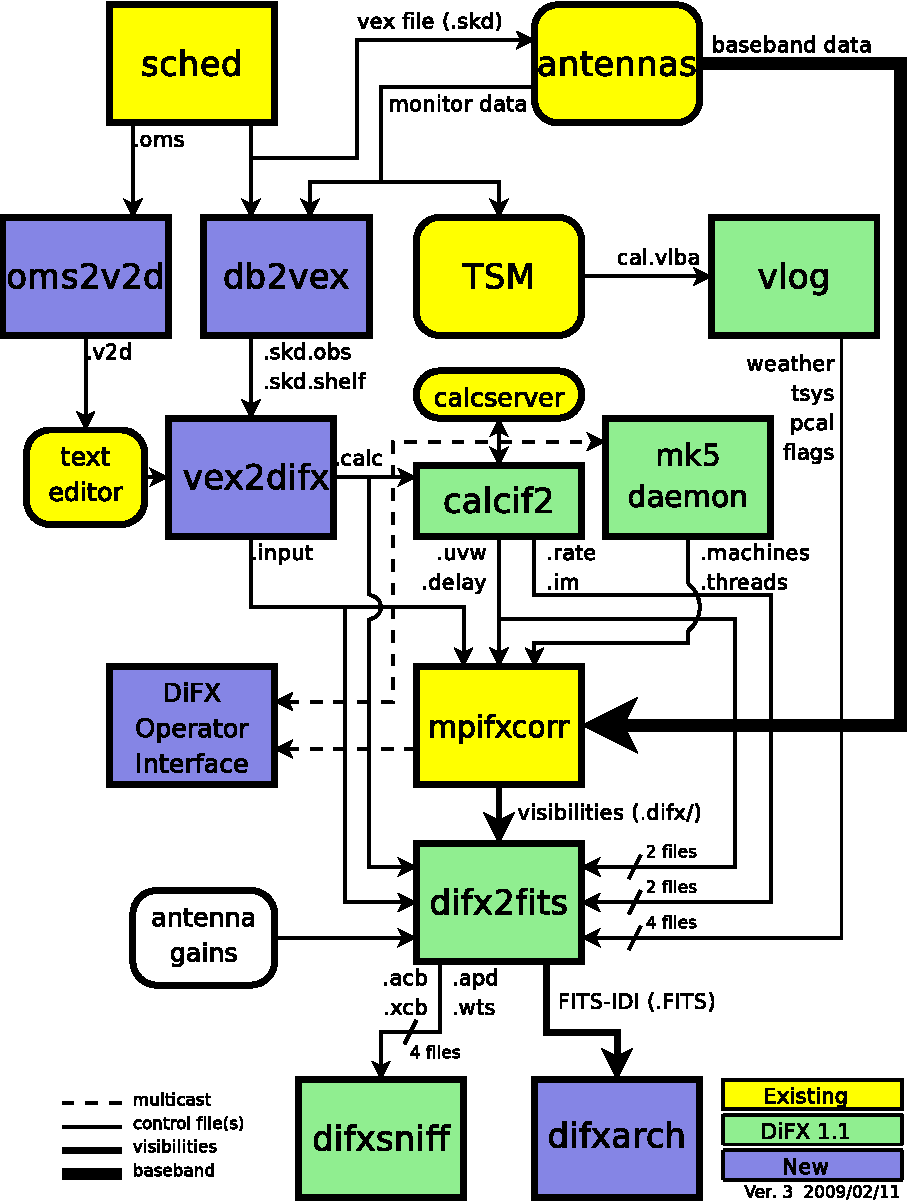
\includegraphics{swcorr_vex_diagram_ver3-crop}}
\caption[blockdiagram]{
{\em The DiFX software correlator block diagram as implemented for the VLBA.}
\label{fig:block}
}
\end{center}
\end{figure}

Past, present, and future versions of DiFX as packaged and used by VLBA operations are described in the following subsections.

% \subsubsection{Supported data formats} \label{sec:formats}


\subsection{NRAO-DiFX 1.0}

Versions 1.0 and 1.1 based correlation on the VLBA hardware correlator job scripts -- the {\tt .fx} files.
This ensures a compatibility period during which both correlators can produce visibilities with expectations of functionally identical results, a feature critical for validation.
This strategy also minimizes the required software effort at its earliest phases.
Version 1.0 came with the following features:
\begin{enumerate}
\item A complete path from {\tt .fx} job scripts to {\tt .FITS} files
\item A command-line only interface
\item Documentation (you are reading it now)
\item Support for VLBA and Mark IV formats
\item Correlation directly off Mark5 modules
\item Support for all projects types except those using special modes, such as pulsars, space VLBI, and near field objects
\item Spectral and time resolution bounded only by practicality
\end{enumerate}
While this version should handle most observations, fast frequency switching and geodesy experiments will produce a large number of output FITS files which may be annoying to observers and the archive.
Version 1.0 was available on February 6, 2008.

\subsection{NRAO-DiFX 1.1}

Version 1.1 builds on version 1.0 and adds the following features:
\begin{enumerate}
\item Used version of {\tt mpifxcorr} that has gone through code merge with the official version
\item Blanking of data replaced by headers (Mark4 format only)
\item Proper data weights
\item Initial Mark5B support
\item Support for oversampled data through decimation
\item Multicast status information for GUI interface
\item Correlation of moving and near field objects
\item Concatenation of multiple output files into a single or multiple FITS-IDI file(s)
\item Better support for jobs with multiple configuration tables
\item Playback off Mark5 modules with missing disks
\item Support for Amazon based Mark5 units
\item Completely replaced the ``Makefile'' system with better integrated alternative
\item Generation of delay model polynomials rather than tables, more like VLBA HW correlator
\item $u, v, w$ values are derived from the delay model (and hence include corrections for aberration, near field observations, and other subtle effects) and are evaluated when writing the FITS file
\item DiFX version accountability
\item Validation of data frames prior to decoding
\item Data evaluation (``sniffing'') built into FITS converter
\end{enumerate}
This version was released on September 3, 2008.
%Features new to version 1.1 are marked with \difxoneone.

\subsubsection{Bugs fixed}

Here are listed some of the more important bug fixes:
\begin{enumerate}
\item The clock offset was used with the wrong sign in the IM table.
\item Printed precision of some important numbers (RA and Dec) was increased.
\item Autocorrelations were ordered incorrectly for observations with a single polarization.
\item The Mark4 format decoder had a 1 day off bug.
\item The Mark4 format decoder had a 64$\times${\it fanout} sample timing offset.
\item Several causes of crashes were fixed; no known crashes remain.
\item Missing VLBA monitor data was handled badly.
\item Due to OpenMPI peculiarity, some processing nodes would get most or all of the work in some cases, which cause the work being done on other nodes to be ignored.  This was fixed by looking for results in a round-robin manner.
\item Integrations that contain data from two adjacent scans are stripped when writing FITS files.
\item Allow FITS files larger than 2GiB in size.
\end{enumerate}

\subsubsection{Known problems}

Known bugs as of the NRAO-DiFX 1.1 release:
\begin{enumerate}
\item The last couple (typically 2) integrations of a job (not a scan) tend to have low weight due to a premature termination of data processing.
\end{enumerate}

\subsection{DiFX 1.5.0}

With DiFX 1.5.0 comes a name change.
Past releases of this series have been known as ``NRAO-DiFX''.
The DiFX community has been largely receptive to the NRAO additions in support of {\tt mpifxcorr} and it was decided that dropping the ``NRAO'' was appropriate.
In some cases the term ``VLBA DiFX'' or ``VLBA DiFX 1.5'' may be mentioned.
These are simply the deployment of DiFX 1.5.0 for the VLBA correlator with some VLBA specific features.
Note that the name given to the VLBA deployment of DiFX is formally ``VLBA DiFX''.

Version 1.5.0 will start allowing correlation of experiments that cannot be represented by {\tt .fx} files and will be based on vex files.
Version 1.5.0 builds on version 1.1 and adds the following features:
\begin{enumerate}
\item Support for using a wide variety of vex files as the basis for correlation.
\item Native ephemeris-based object trajectories are supported.
\item Pulsar gating is supported.
\item Pulsar binning is supported, but not cleanly yet.
\item A graphical user interface is available for correlator operators.
\item The multicast system is fully implemented and is used monitor and control correlation and other operations.
\item Mark5B formatted data, including its 2048 Mbps extension, is supported.
\item The VLBA DiFX Operations Plan \cite{opsplan} is implemented, including interface to the VLBA archive.
\end{enumerate}
Non-NRAO users of DiFX 1.5.0 will still be able to use the tools provided but may not be able to take full advantage of the database back-end without some customization; it is the aim of this document to point out cases where the database is required.
Many of the programs described in previous versions of this document will be upgraded or overtaken by more capable replacements.

Release of DiFX 1.5.0 was announced on June 25, 2009.

%Features new to the 1.5 series are marked with \difxonefive.

\subsubsection{Bugs fixed}

Here are listed some of the more important bug fixes:
\begin{enumerate}
\item A rounding issue in {\tt mpifxcorr} occasionally caused the wrong source's UVWs to be assigned.
\item Lower side band data would come out of the sniffer portion of {\tt difx2fits} with the wrong sign for phase, rate, and delay.
\item Different rounding was used to generate start times for {\tt .input} and {\tt .calc} files.
There are no severe consequences of this issue.
\item Scaling in pulsar gating has been made more sane.
\end{enumerate}

\subsection{DiFX 1.5.1}

DiFX 1.5.1 is mostly a bug fix update to version 1.5.0, but with a few new features.
The new features include:
\begin{enumerate}
\item Option to force job breaks (with the break parameter) has been added to {\tt vex2difx}
\item Time/date formats other than decimal MJD are now accepted by {\tt vex2difx}
\item Specification of data files to correlate (rather than Mark5 units) is supported in {\tt vex2difx}
\item Specification of network parameters in {\tt vex2difx} to allow correlation of eVLBI projects
\item {\tt difx2fits} produces a new output file with suffix {\tt .jobmatrix} provides the user with a better idea of the mapping of jobs into {\tt .FITS} files
\item A {\tt vex2difx} mode for generating DiFX files useful for determining pulsar phase has been added
\item EOP values can now be provided within the {\tt .v2d} file
\item Upcoming FITS-IDI keyword WEIGHTYP populated
\item Zero-weight data is not written from {\tt mpifxcorr}
\item New utility {\tt checkdir} to look for oddities in Mark5 module directory files
\end{enumerate}

\subsubsection{Bugs fixed}

Here are listed some of the more important bug fixes:
\begin{enumerate}
\item Concatenation of jobs in the creation of {\tt .FITS} files does the right thing for cases where the antenna subsets change and where antenna reordering is done.
\item The Pulsar Gate Model (GM) {\tt .FITS} file table is now correctly populated for pulsar observations.
\item Autocorrelations are written for each pulsar bin
\item The FXCORR simulator mode of {\tt vex2difx} now selects the correct reference time for antenna clock offsets.
\item A work-around for a Streamstor problem has been added that should improve reliability in Mark5 module correlation when a change in bank is needed.
\item The sign of clock offsets in vex files has been reversed to follow the vex standard
\item Jobs are split at leap seconds
\item LBA data formats are handled more correctly in {\tt vex2difx}
\item The model generator ({\tt calcif2}) now respects polynomial parameters interval and order given on the command line.
\end{enumerate}

DiFX~1.5.1 was made available via subversion on Sep 8, 2009.

\subsection{DiFX 1.5.2}

DiFX~1.5.2 is mostly a bug fix update to version 1.5.1, but with a few new features.
This version of DiFX comes with the following components (and versions): calcif2 (1.1), calcserver (1.2), difx\_db (1.12; NRAO-only), difx2fits (2.6.1), difx2profile (0.1), difxio (2.12.1), difxmessage (0.7), mark5access (1.3.3), mk5daemon (1.2), mpifxcorr (1.5.2), vex2difx (1.0.2), and vis2screen (0.1).
The new features include:
\begin{enumerate}
%\item Primitive support for single-thread VDIF format data
\item Support unmodulated VLBA format data with new pseudo-format ``VLBN''
\item {\tt mpifxcorr} now warns when difxmessage is in use so the user knows why no messages appear on the screen
\item New utility {\tt difxcalculator} in the {\tt difxio} package
\item eVLBI support within {\tt vex2difx}
\item Vastly improved real-time correlation monitoring
\item New utility {\tt diffDiFX.py} to compare two DiFX output files
\item Improved and more consistent error messages (and some of them are now documented!)
\item {\tt vex2difx} now operates in strict parsing mode by default
\item Additional user feedback to indicate suspicious or bad {\tt .polyco} and {\tt .v2d} files
\item {\tt calcif2} warns if any NaNs or Infs are produced
\item Clock adjustments are easier now with {\em deltaClock} and {\em deltaClockRate} parameters in the {\tt vex2difx} antenna settings
\end{enumerate}

\subsubsection{Bugs fixed}

\begin{enumerate}
\item Improve timestamp precision (thanks to John Morgan)
\item The {\tt vlog} program (used at NRAO only, I think) misparsed the pulse cal information in some cases
\item Fixed memory leak in {\tt difx2fits} when combining a large number of jobs
\item Improved FXCORR simulation mode in {\tt vex2difx}
\item Mark5 directory reading systematically generates unique names for all scans even when two scans have the same name
\item Improve reporting of Mark5 errors during playback and change alert severity to be more appropriate
\item Don't overblank certain Mark4 modes (thanks to Sergei Pogrebenko for the bug report)
\item Vex `data valid' period now properly respected
\item Vex clock table tolerance issue corrected
\item Changes in Mark5 mode should be safer (note that currently {\tt vex2difx} never exercises multiple modes in a single job)
\item When making the cross spectrum sniffer plots, respect the reference antenna
\item Improved pulsar polynomial file error checking is performed
\item Amplitude-phase-delay (APD) sniffer plots always have refant first when multiple refants are supplied
\item Project name should now appear on sniffer APD plots
\item Mark5 units now send status information even when no playback is occuring (eliminating the incorrect {\tt LOST} state issue as displayed in the DOI)
\end{enumerate}

\subsubsection{Known problems}

\begin{enumerate}
\item Extensive use in VLBA operations has shown that occasional data dropouts of one or more antenna, sometimes in a quasi-repeatable manner, affect completeness of some jobs.  
It is not clear exactly what the cause is at this point, however its cure is a high priority.
\item Loss of a few FFTs of data will occur in rare circumstances.
\item Clock accountability is poor when jobs containing multiple clock models for antennas are combined.
\end{enumerate}

DiFX~1.5.2 was made available via subversion on Jan 20, 2010.

\subsection{DiFX~1.5.3}

DiFX~1.5.3 is mainly intended as a bug fix update to version~1.5.2, though some new features have made their way into the codebase.
This version of DiFX comes with the following components (and versions): calcif2 (1.3), calcserver (1.3), difx\_db (1.13; NRAO-only), difx2fits (2.6.2), difx2profile (0.2), difxio (2.12.2), difxmessage (7.2), mark5access (1.3.4), mk5daemon (1.3), mpifxcorr (1.5.3), vex2difx (1.0.3), and vis2screen (0.2).
Many changes are motivated by issues found running DiFX full time in Socorro.

The new features include:
\begin{enumerate}
\item Mark5 directory ({\tt .dir}) files can contain {\tt RT} on the top line to indicate the need to play back using {\em Real-Time} mode.
\item {\tt difxqueue} (NRAO only) now takes an optional parameter specifying the staging area to use.
\item New Mark5 diagnostic programs ({\tt vsn} and {\tt testmod}) introduced to wean off the use of the {\tt Mark5A} program.
\item {\tt mk5daemon} can now mount and dismount USB and eSATA disks through mk5commands.
\item {\tt mk5cp} now makes the destination directory if it doesn't exist.
\item {\tt mk5daemon} will now warn if free disk space is getting low.
\item {\tt db2vex} (NRAO only) now allows field station logs to be provided.  As of now, only media VSNs are extracted.
\item Playback off Mark5 units has been made more robust with better error reporting.
\item New utility {\tt m5fold} that can be used to look at repeating signals in baseband data total power (e.g., switched power)
\item {\tt vex2difx} now supports job generation in cases where upper side band was observed at one antenna and lower sideband at another.
\end{enumerate}

\subsubsection{Bugs fixed}

\begin{enumerate}
\item Don't unnecessarily drop any FFTs of data.
\item Sub-integrations longer than one second could cause integer overflows.
\item Fix bug in {\tt vex2difx} where jobs were not split at clock breaks.
\item {\tt difx2fits} was guilty of incorrect clock accoutability after a clock change at a station when merging multiple jobs.  Worked around by not allowing such jobs to merge.
\item {\tt db2vex} (NRAO only) warns when more than one clock value is found for an antenna.
\item Mark5 unit bank switches now routinely call {\tt XLRGetDirectory()} to work around a newly discovered bug in the StreamStor software.
\item A couple possible memory leaks in the mark5access library were fixed (thanks Alexander Neidhardt and Martin Ettl).
\item Lots of compiler warnings quashed (mostly of the ``unused return value'' kind).
\item Olaf Wuchnitz found two FITS file writing problems in {\tt difx2fits} dating back to code inherited from FXCORR!
\item Two more digits are retained for the time and one more digit is retained for amplitude information in the {\tt .apd} and {\tt .apc} sniffer files.
\item Some bugs related to replacement of special characters by ``entities'' in XML messages are fixed.
\item New traps are in place in many places to catch string overruns.
\item Fix for writing {\tt .calc} files with more than one ephemeris driven object.
\item {\tt vex2difx} would get {\em very} slow due to constantly sorting a list of events.  Now this list is only sorted when necessary, drastically speeding it up.
\item The {\tt RCfreqId} parameter in the difxdatastream structure (in difxio) was used with two different meanings that are normally the same.  Cases where they differred caused exceptions.  Fixed in difxio and difx2fits. (Thanks to Randall Wayth for leading to the discovery)
\item {\tt difx2fits} would assign a bogus {\tt .jobmatrix} filename when not running the sniffer.
\item {\tt vex2difx} could get caught in an infinite loop when making jobs where two disk modules had zero time gap.
\item {\tt difx2fits} used a bad config index when making the puslar GM table when multiple configs were present.
\item Within {\tt mpifxcorr} an extra second was added to the validity period for polycos to ensure no gap in coverage.
\item {\tt mk5dir} would add correct the date improperly for Mark4 formats after beginning of 2010.
\item Lots of fixes for building FITS files out of a subset of baseband recorded channels.
\item FITS files now support antennas with differing numbers of quantization bits.
\item Lots of Mac OS/X build issues fixed.
\end{enumerate}

DiFX 1.5.3 was released on April 16, 2010.

\subsection{DiFX~1.5.4}

DiFX~1.5.4 is likely the last 1.5 series formal release of DiFX, though an additional release could be made if demand is there.

The new features include:
\begin{enumerate}
\item {\tt difx2fits} can now produce FITS files with only a subset of the correlated sub-bands.
\item {\tt difx2fits} can be instructed to sniff on an arbitrary timescale.
\item The {\tt makefits} wrapper for {\tt difx2fits} now respects a -B option for phase bin selection.
\item {\tt difxio} has improved checking that prevents merging of jobs with incompatible clocks.
\item {\tt difxio} now maintains a separate clockEpoch parameter for each antenna.
\item {\tt difxStartMessage} now contains DiFX version to run, allowing queued jobs to be run under different DiFX versions.
\item The curses utilities {\tt mk5mon} and {\tt cpumon} now catch exceptions and can be resized without infecting the terminals they are run in.
\item New sub-library called mark5ipc added that provides a semaphore lock for Mark5 units.
\item The {\tt testdifxmessagereceive} utility can now filter on message types.
\item Support for SDK9 throughout (e.g., in {tt mpifxcorr}, {\tt mk5daemon}, and other utilites).
\item Support for new Mark5 module directory formats (Haystack Mark5 memo 81).
\item Several new Mark5 utilities to make up for Mark5A functionality that will not longer be available: {\tt vsn}, {\tt testmod}, {\tt recover}, {\tt m5erase}.
\item {\tt mk5cp} can now copy data based on byte range.
\item Many programs directly talking to the StreamStor card of Mark5 units use WATCHDOG macros for improved diagnostics when problems occur.
\item More protection against incomplete polyco files added to {\tt mpifxcorr} (Note: should add this to {\tt vex2difx} as well).
\item The GUI can now spawn different DiFX versions at will through the use of difxVersion parameter in the DifxStartMessage and wrapper scripts.
\item {\tt difx2fits} can now convert LSB to USB for matching purposed.  When used, all LSB sub-bands must have corresponding USB sub-bands on one or more other antenna.
\item {\tt mark5access}-based utilities (e.g., {\tt mp5spec}) can now read from stdin.
\item New utility {\tt mk5cat} can send data on a Mark5 module to stdout.
\end{enumerate}

\subsubsection{Bugs fixed}

\begin{enumerate}
\item Only alt-az telescopes received the correct model.  Fixed.  Note that CALC and FITS-IDI don't have a good match between their sets of allowed mount types.
\item {\tt difx2fits} now properly propagates quantization bits on a per antenna basis.
\item Logic errors in {\tt difxio} would confuse {\tt difx2fits} in cases where different antennas use different frequency setups.  Fixed.
\item Weights are blanked in {\tt difx2fits} prior to populating each record, preventing screwy weights for unused sub-bands.
\item {\tt vex2difx} would sometimes hang or not converge on job generation.  Fixed.
\item {\tt vex2difx} now doesn't assume source name is same as vex source def identifier.
\item {\tt mpifxcorr} generated corrupted weights and amplitudes when post-FFT fringe rotation was done.  Fixed.
\end{enumerate}

\subsection{Known bugs}

\begin{enumerate}
\item Tweak Integration Time feature of {\tt vex2difx} often does the wrong thing.
\end{enumerate}

DiFX 1.5.4 was released on October 12, 2010.

\subsection{DiFX 2.0.0}

DiFX 2.0.0 is based on an upgraded {\tt mpifxcorr} that breaks {\tt .input} file compatibility with the 1.0 series.
This new version will allow more flexible correlation of mis-matched bands and correlation at multiple phase centers along with general performance improvements.
Development of the 2.0 capabilities will occur in parallel with the 1.0 series features.

\subsubsection{New features}

\begin{enumerate}
\item Pulse cal extraction in {\tt mpifxcorr}.
\item Massive multi-phase center capabilitiy.
\item New utitility {\tt zerocorr} added.
\item External pulse cal extraction utility {\tt m5pcal} added.
\item DiFX output format is all-binary, meaning speed and disk savings
\end{enumerate}

\subsection{Known bugs}

\begin{enumerate}
\item Zoom band support has multiple problems.
\end{enumerate}

DiFX 2.0.0 was released on October 12, 2010.

\subsection{DiFX 2.0.1}

DiFX 2.0.1 is a bug fix and clean-up version in response to numerous improvements to DiFX 2.0.0.
There are a number of new features as well.

\subsubsection{New features}

\begin{enumerate}
\item New utility {\tt checkmpifxcorr} to validate DiFX input files
\item Switched power detection in {\tt mpifxcorr}
\item Early multi-thread VDIF format support
\item RedHat RPM file generation for some packages (can extend to others on request)
\item Improvements to method of selecting which pulse cal tones get propagated to FITS
\item Initial complex sampling support
\item Improved locking mechanism for direct mark5 access (using IPC semaphores; difxmessage)
\end{enumerate}

\subsubsection{Bug fixes}

\begin{enumerate}
\item Fix model accountability bug in difx2fits when combining jobs
\item Numerous fixes for zoom bands (in {\tt mpifxcorr}, {\tt vex2difx} \& {\tt difx2fits})
\item Native Mark5 has improved stability for cranky modules
\item Numerous fixes for DiFX-based phase cal extraction (mostly in {\tt difx2fits}, mostly for multi-job)
\item Fractional bit correction for a portion of lower sideband data got broken in difx 2.0.0. Fixed.
\item Migrate {\tt difxcalculator} to DiFX 2; was not complete for DiFX 2.0.0
\end{enumerate}

DiFX 2.0.1 was released on June 24, 2011.

\subsection{DiFX 2.1}

\subsubsection{New features}

\begin{enumerate}
\item Mark5-based correlation: easy access to S.M.A.R.T.\ data (can be viewed with getsmart)
\item Mark5-based correlation: emit multicast message containing drive statistics after each scan
\item VSIS interface added to mk5daemon
\item Support for non power-of-2 FFT lengths
\item New utilities: {\tt mk5map} (limited functionality), {\tt fileto5c}, {\tt record5c}
\item Remote running of {\tt vex2difx} from {\tt mk5daemon}
\item Multithread VDIF support enabled for the data sources FILE and MODULE, including stripping of non-VDIF packets
\item New features added to existing utilities:
\begin{itemize}
\item {\tt mk5cp}: copy without reference to a module directory
\item {\tt mk5cp}: ability to send data over ssh connection
\item vsn: get SMART data from disk drives
\end{itemize}
\item e-Control source code analysis (Martin Ettl, Wettzell)
\item Restart of correlation is now possible
\item {\tt difx2fits}: -0 option to write minimal number of visibilities to FITS
\item {\tt difx2fits}: write new RAOBS, DECOBS columns in source table
\item tweakIntTime option to {\tt vex2difx} has been re-enabled
\item {\tt diffDiFX.py} can now cope with two files that don't have exactly the same visibilities (i.e., some visibilities are missing from one file)
\item {\tt plotDiFX.py} and {\tt plotDynamicSpectrum.py} now have better plotting and more options
\item New FAKE datastream type for performance testing
\item Espresso, a lightweight system for managing disk-based correlation, has been added to the DiFX repository. 
\item Option to correlate only one polarization has been added.
\item {\tt mk5dir} can now produce {\tt .dir} file information for VDIF formatted data.
\item Add NRAO's sniffer plotters to the repository.
\end{enumerate}

\subsubsection{Bug fixes}

\begin{enumerate}
\item LBA format data now scaled roughly correctly (removing the need for large ACCOR corrections).
\item There was a bug when xmaclength was $>$ nfftchan for pulsar processing. This has been corrected.
\item guardns was incorrectly (overzealously) calculated in mpifxcorr.
\item {\tt Mk5DataStream::calculateControlParams: bufferindex>=bufferbytes} bug fixed.
\item Low weight reads could result in uninitialized memory; fixed.
\item Streamstor {\tt XLRRead()} bug work-around installed several places (read at position 0 before reading at position $> 0$). This is thought not to be needed with Conduant SDK 9.2 but the work-around has no performance impact.
\item Fix to pulse calibration data ordering for LSB or reordered channels.
\item Pulse cal amplitude now divided by pulse cal averaging time in seconds.
\item Pulse cal system would cause crash if no tones in narrow channel. Fixed.
\item Zoom band support across mixed bandwidths (see caveat below).
\item Fix for spurious weights at end of jobs (untested\ldots)
\item Mixed 1 and 2 bit data are handled more cleanly
\item mpifxcorr terminates correctly for all short jobs.  Previously it hung for jobs with a number of subints between nCores and $4 \times$ nCores
\item Correctly scale cross-correlation amplitudes for pulsar binning when using {\tt TSYS} $>0$ (accounts for varying number of samples per bin c.f.\ nominal)
\item Lower side-band pulse cal tones had sign error.  Fixed.
\end{enumerate}


DiFX 2.1 was released on May 25, 2012.


\subsection{DiFX 2.1.1}

DiFX 2.1.1 was a minor patch release to fix a scaling issue with autocorrelations of LBA-format data in mpifxcorr.

DiFX 2.1.1 was committed as a patch to DiFX 2.1 on June 7, 2012.

\subsection{DiFX 2.2}

\subsubsection{New features}

\begin{enumerate}
\item {\tt calcif2}: ability to estimate delay polynomial interpolarion errors
\item Support for a ``label'' identifier for a local version of DiFX that will help discriminate exact version used.
\item Faster Mark5 directory reading
\item Faster VDIF corner turning through customized bit shifting functions
\item {\tt mpifxcorr} can now be built without Intel Integrated Performance Primitives, though resulting in a slower correlator.
\item {\tt vdifio}: several new VDIF manipulation and processing utilities added: {\tt vmux}, {\tt vsum}, {\tt vdifd}, {\tt vdifspec}, {\tt vdiffold}, {\tt vdifbstate}
\item {\tt difxbuild}: a new installation program
\item {\tt difxspeed}: a program to benchmark and help optimize DiFX
\end{enumerate}

\subsubsection{Bug fixes}

\begin{enumerate}

\item Mutex locking bugfix for very short jobs
\item Prevent MODE errors when a datastream runs out of data well before the end of a job
\item {\tt calcif2}: fix azimuth polynomial generation in case of wrap
\item Fix for FITS file generation for mixed sideband correlation
\item {\tt difx2fits} now uses appropriate gain tables for S and X band in S/X experiments (Thanks to James Miller-Jones for reporting)
\item {\tt difx2fits}: correct pcal, weather, tsys and flag data for observations crossing new year
\item Fixed scaling of autocorrelations for LBA format data
\item 0.5 ns wobble in delays for 2 Gbps Mark5B data fixed
\item Fix bug preventing subintegrations longer than 1 second. Now 2 seconds is allowed (this limit comes from signed integer number of nanoseconds).
\item Weights corrected in cases where two setups differening only by pcal setup were correlated against each other
\item Quashed data and weight echos that would occur for about 1 integration at the beginning of each scan for datstreams that ran out of data before end of job.
\item The multicast (diagnostic) weights were low or zero in case of frequency selection (zoom band or freqId selection). Fixed.
\item {\tt mark5access}: fix (non)blocking issue when receiving data from {\em stdin}


\end{enumerate}


DiFX 2.2 was released on June 12, 2013.



\subsection{DiFX 2.3}

\subsubsection{New features}

\begin{enumerate}

\item mpifxcorr: LO offsets are now corrected in the time domain when fringe rotation is also done in the time domain (the usual mode), allowing considerably larger LO offsets without decorrelation
\item mpifxcorr: Working polarization dependent delay and phase offsets
\item mpifxcorr: Experimental linear2circular conversion
\item mpifxcorr: Complex Double sideband (RDBE/Xcube) sampling support (Note: things are not perfect here; wait for 2.4 for real use)
\item mpifxcorr: new file/Mark5 based VDIF/Mark5b datastream (faster and more robust)
\item mpifxcorr: implement work-around for buggy kernel-driver combinations; Mark5 read sizes >20 MB now allowed
\item utilities: some new command line tools for Mark5B and VDIF files (vsum, mk5bsum, vmux, mk5bfix)
\item new options for passing calibration (Walter B: memo forthcoming)
\item Hops updated to version 3.9

\end{enumerate}

\subsubsection{Bug fixes}

\begin{enumerate}

\item mpifxcorr: Datasteam buffer send size now calculated correctly for complex sampled data
\item mpifxcorr: Avoid very rare bug where combination of geometric delay and data commencing mid-subint meant one invalid FFT might be computed
\item mpifxcorr: multicast weights are now computed correctly for mixed-sideband correlation
\item mpifxcorr: fixed bug where some autocorrelations were not saved in a mixed-sideband correlation
\item mpifxcorr: fixed bug where send size could be computed incorrectly by 1-2 bytes for
\item Mark4/VLBA/Mark5B/VDIF formats, potentially resulting in very small amounts of data loss

\end{enumerate}

DiFX 2.3 was released on January 18, 2014.


\subsection{DiFX 2.4}

\subsubsection{New Features}

\begin{enumerate}

\item mpifxcorr
\begin{itemize}
\item Support a FAKE correlation mode for multi-threaded VDIF.
\item The mpifxcorr produced PCAL files have had a format change that allows unambiguous interpretation across all use cases.
\item Add network support (TCP, UDP and Raw Ethernet) for multi-threaded VDIF:
1.\  TCP and UDP variants not tested yet;
2.\  raw Ethernet variant is used for the VLITE project.
\item Support updated Mark5 module directories.
\item Better checking that Mark5 data being processed matches what is expected.
\item Improved Mark5B decoding:
1.\ Mark5B data streams are now filtered for extra or missing data;
2.\ packets with invalid bit (actually the TVG bit) set replace missing data;
3.\ this means any valid Mark5B data with the TVG bit set will not correlate.
\item Information about each Mark5 unit used in ``native mode'' is emitted at start of jobs so it can be logged.
\item Ultra-low frame rate VDIF data was affected by allowing a long ``sort window'' in the VDIF multiplexer.  
This has been reduced to 32 frames and seems to work fine for all bandwidths now.
\end{itemize}

\item difx2fits
\begin{itemize}
\item Slightly improved compliance with the FITS-IDI convention:
1.\ invalid Tsys values become NaN, not 999;
2.\ populate {\tt DELTAT} keyword in ModelComps table.
\end{itemize}

\item difxio
\begin{itemize}
\item Support for X/Y polarization correlation.  Many fundamental issues with       
  linear polarization remain though: 
1.\ this does not support in a meaningful way Linear*Circular correlations;
2.\ there is a terminology gap in many bits of software and file formats that confuses X/Y with H/V polarization bases;
3.\ the intent of this support is for short baselines (VLITE).
\end{itemize}

\item mark5access
\begin{itemize}
\item Support for "d2k" mode in Mark5B format (swapped sign and mag bits).
\item fixmark5b() function fixed for case that fill pattern is seen at the 1 second transition.
\item Make use of the TVG bit as an "invalid frame" indicator for Mark5B data.
\item m5bstate: support complex sampled data
\end{itemize}

\item mk5daemon
\begin{itemize}
\item New utility mk5putdir: reads a binary file and replaces a Mark5 directory with it.
\item mk5dir: when reading the directories, saves a copy of the binary representation in case it is needed later (perhaps via mk5putdir)
\item Reworked mark5 module directory support, including support for many new variants of the directory format.
\item mk5erase will save a ``conditioning report'' to {\tt \$MARK5\_CONDITION\_PATH} if that environment variable is set.
\end{itemize}

\item vdifio
\begin{itemize}
\item Fairly large change to the API.  Please read the ChangeLog for details.
\end{itemize}

\item vex2difx
\begin{itemize}
\item Respect the record enable bit in the SCHED block.  If that value is 0 no correlation will be attempted for that antenna.
\item Bug fixes preventing some LSB/zoom bands from being correlated.
\item Complex data type and number of bits are now read from vex file.
\end{itemize}

\end{enumerate}

\subsubsection{Bug fixes}

\begin{enumerate}

\item A ``jitter'' of 0.5~ns when using 2Gbps Mark5B format was fixed.  A fix was back-ported to DiFX 2.3.
\item A similar jitter was corrected for high frame rate VDIF (problem identified by the VLITE project)
\item Fix case of intermittant fringes that was due to incorrect assumption about the sizeof(unsigned long): 32 bits on a 32-bit system vs. 64 bits on a 64-bit system.
Some other variable types were changed for long term type safety
\item Fix off-by-one in correlation using LSB and zoom bands together.

\end{enumerate}

\subsection{DiFX 2.5.1}

\subsubsection{New features}

\begin{enumerate}

\item Innitial support for correlating Mark6. This is still much a work in progress.
\item Multiple datastreams per antenna supported via {\tt vex2difx}
\item New delay model program: difxcalc11.? No longer requires calcserver.
\item Support for more than 6 days of EOP values.
\item ``Union mode'' in difx2fits allows merging of correlation output that uses different setups. Some restrictions apply. Designed for GMVA and RadioAstron use.
\item Improved VDIF support: wider range of bits/threads, support for multi-channel, multi-thread VDIF, support for complex multi-thread VDIF
\item Support for new VDIF Extended Data Version 4 which is useful for multiplexed VDIF data. See: \url{http://vlbi.org/vdif/docs/edv4description.pdf}
\item Python bindings for vdifio and mark5access
\item mpifxcorr: per-thread weights implemented
\item Automatic selection of arraystride by mpifxcorr if set to zero; this is done per-datastream.? Very useful for correlation of ALMA data or others with non-standard sample rates.
\item Automatic selection of xmacstride by mpifxcorr if set to zero
\item Automatic selection of guardns by mpifxcorr if set to zero
\item mpifxcorr can now operate with unicast messages instead of multicast. Useful in some situations where multicast is not
supported.
\item New ``dirlist'' module/file directory listing format. 
\item {\tt mk5cp} append mode to resume interrupted copy
\item ALMA support in HOPS: non-power-of-two FFTs, up to 64 freq.\ channels, full linear/circular/mixed polarization support
\item HOPS improvemetns for VGOS through improved manual phase cal support
\item New package: polconvert. Used to post-correlation convert from linear to circular polariations
\item New package: autozoom. Helps a user develop {\tt .v2d} file content when setting up complicated zoom band configurations.
\item New package: datasim: generate baseband data suitable for simulated correlation
\item Improved error reporting in many places

\end{enumerate}

\subsubsection{Bug fixes}

\begin{enumerate}

\item fix for incorrect reporting of memory use by mpifxcorr (needed longer int sizes)
\item dataweights would sometimes be incorrect after abrupt ending of data from a datastream.
\item FITS-IDI files produced by difx2fits more standards compliant; fix problem that caused AIPS task VBGLU to fail.
\item Several segfaults across a number of programs/utils now are caught and provide useful feedback. 

\end{enumerate}

\subsubsection{Caveats}

\begin{enumerate}

\item Various changes made between DiFX 2.4 and 2.5 are not API-compatible. Please don't mix packages from these two releases.  If you have non-DiFX software that links against the DiFX libraries, be sure to recompile them. A small number of changes may result in need to restructure such code.
\item Unlike previous DiFX releases, each tagged version will be its own SVN copy. If the number of minor releases within the 2.5 series gets large, some (reversible) pruning of the SVN repository may occur.  There has been some debate about the best tagging strategy: bring any strong opinions to the Bologna meeting, where further changes to release and tagging policies can be discussed if needed.

\end{enumerate}


\section{DiFX 2.5.2}

\subsection{Bug fixes}

\begin{enumerate}

\item Fixes for the HOPS 'rootid' rollover.  The new rootcode is a conventional base-36 timestamp in seconds from the start of the new epoch (zzzzzz in the old epoch).  This will last until 2087.
\item Major fixes/improvements to PolConvert for use with ALMA by the EHTC and GMVA.

\end{enumerate}


\section{DiFX 2.5.3}

\subsection{Updates}

\begin{enumerate}

\item genmachines
\begin{itemize}
  \item r8264 genmachines and mark6 datastream updates
  \item r8357 add mark6 activity message to mark6 datastream
  \item r8409 allow multiple nodes to serve as datastream nodes for FILE based-data in the same location
\end{itemize}
\item hops 3.19 new features
\begin{itemize}
  \item increased the number of allowed frequency ``notches'' to ridiculous levels
  \item an “ad hoc” data flagging capability to allow improved time / channel data selection for fringing
  \item a capability to dump all the information on the fringe plots into ascii files for “roll your own” plotting
  \item removed obsolete {\tt max\_parity}
  \item introduced {\tt min\_weight} (to discard APs with very little correlated data in support)
  \item vex2xml, a program that converts VEX (v1.5) into XML to allow easy parsing via standard XML parsers.
  \item added {\tt type\_222} to save control file contents, enabled by keyword {\tt gen\_cf\_record}.
\end{itemize}
    polconvert to v1.7.5 (mostly minor bug fixes and robustifications)
\end{enumerate}

DiFX 2.5.3 was released on March 28, 2019.


\section{DiFX 2.6.1}

\subsection{New features}

\begin{enumerate}
\item Improved VDIF support
\begin{itemize}
  \item Increased robustness in processing VDIF data with many gaps
  \item Improvements in processing VDIF with frame sizes very different from 5000 bytes
  \item  New in-line reordering functionality via vdifreader…() functions; allows operation on more highly skewed VDIF files
\end{itemize}
\item mpifxcorr {\tt .input}, {\tt .calc}, {\tt .threads}, and pulsar files are now only read by the head node
\item mpifxcorr can be provided a new stop time via a DifxParameter message; results in clean shutdown at that time.
\item mpifxcorr can extract pulse cals with tone spacing smaller than 1 MHz
\item Support for Intel Performance Primitives version > 9 (specfically IPP 2018 and 2019)
\begin{itemize}
  \item These newer IPP versions are more readily available than earlier versions
\end{itemize}
\item Improved support for Mark6 playback
\begin{itemize}
  \item Mark6 activity messages in difxmessage
  \item Support in genmachines with updated mk5daemon
  \item Support playback of Mark5B data on Mark6
  \item New and improved mark6 utilities
\end{itemize}
\item difx2fits: populate antenna diameters and mount types for antennas known to the difxio antenna database
\item difx2fits: in verbose mode, explain why files are being split
\item difx2fits: new options for merging correlator jobs run with different clock models
\item vex2difx: new parameter {\tt exhaustiveAutocorrs} can be used to generate cross-hand autocorrelations even when the two polarizations for an antenna come from different datastreams
\item difx2mark4: support multiple bandwidths in one pass
\item hops: to rev 3.19 (see notes on 2.5.3 above for details on several new and useful features)
\item polconvert: to rev 1.7.5 (see notes on 2.5.3 above for details)
\end{enumerate}

\subsection{Bug fixes}

\begin{enumerate}
\item mpifxcorr: Retry on NFS open errors of kind: ``EAGAIN Resource temporarily unavailable''
\item mpifxcorr: Fix weight issue when the parameter {\tt nBufferedFFTs} $ > 1$
\item startdifx/genmachines: Fixes for cases when multiple input files are provided
\item Python 2 scripts now explicitly call python2
\item vex2difx: allow up to 32 IFs (was 4) and warn when this is exceeded
\item vex2difx: support units in the clock rate (e.g., usec/sec); in general support time in the numerators.
\item Sun RPC is on its way out; support for ``tirpc'' added to calcif2 and calcserver
\end{enumerate}

\subsection{Caveats}

\begin{enumerate}
\item Moved “mark6gather” functions from vdifio to mark6sg; this changes the order of dependencies!
\item Various changes made between DiFX 2.5 and 2.6 are not API-compatible. Please don't mix packages from these two releases. If you have non-DiFX software that links against the DiFX libraries, be sure to recompile them. A small number of changes may result in need to restructure such code.
\item There is some suspicion that correlation of very narrow bandwidth VDIF modes on Mark6 media can result in premature termination of datastreams.
\item The {\tt .threads} file must now exist; previously (before the change to only have manager read these files), a missing {\tt .threads} file would cause each core process instance to have a single thread.
\item difx\_monitor won't compile with IPP $\ge 9$
\end{enumerate}

DiFX 2.6.1 was released on August 28, 2019.


\section{DiFX~2.6.2}

\subsection{New features}
\begin{enumerate}
\item Python parseDiFX package added
\end{enumerate}

\subsection{Updates}
\begin{enumerate}
\item HOPS updated to version 3.21
\item PolConvert updated to version 1.7.8
\item Former FTP access to CDDIS servers changed to FTP-SSL (geteop.pl)
\end{enumerate}

\subsection{Bug fixes}
\begin{enumerate}
\item mpifxcorr: Fix correlation of Complex LSB data, restore fringes. Note: DiFX 2.5.x and 2.6.1 treated Complex LSB as if Complex USB, while Trunk prior to r9647 05aug2020 treated LSB nearly correctly except for a off-by-one channel bug
\item difx2mark4: Fix seg-fault in createType3s.c when a station has only a single entry in the PCAL file
\item difx2mark4: Remove unneeded debugging statement (calling d2m4\_pcal\_dump\_record())
\item difx2mark4: Update createType3s.c to add support for DiFX PCAL files generated from station data where each data-stream thread resides in a separate file (multi-datastream support). This separates the code reading the PCAL files from the code filling the type-3 records so that tone records from multiple data streams can be merged before populating the type-309s
\item difx2mark4: Update createType3s.c to remove support for DiFX version-0 PCAL files
\item difx2mark4: Add support for 10 MHz p-cal tone spacing (needed by VGOS at Yebes)
\item difx2mark4: Significantly increase hardcoded array sizes (difx2mark4.h: NVRMAX 8M, MAX\_FPPAIRS 10k, MAX\_DFRQ 800) as required for EHT2018
\item difx2mark4: Fix a bounds check, permit tabs in VEX file
\item difx2fits: Fix FITS PH table having missing or superfluous pcal records when one correlates multi-datastream antennas, or not all recorded frequencies, or multiple zooms per recorded frequency
\item mark6gather: Fix poor weights in native Mark6 correlation for VDIF frame sizes not equal to 5032 bytes
\item difxio: Fix PCal tone frequency rounding bug on some platforms
\item difxio: Cope with recorded bands that lack PCal tones, e.g., 200 MHz PCal spacing of KVN with say 32 MHz recorded bands
\item calc11: Dave Gordon provided ocean loading params at EHT stations
\item calc11: Increased the number of field rows supported in .calc files
\item vex2difx: Fix internal merge of SamplingType (real, complex) when info found in VEX and/or v2d file
\item Minor changes to oms2v2d and vexpeek
\item More IPP versions supported
\item Minor issues with vis2screen fixed
\item Fixed build failure with gcc defaults
\item Python3 support in many/most places
\end{enumerate}

\subsection{Caveats}
\begin{enumerate}
\item difx2mark4: Some LSB-LSB baselines do not get converted in mixed-sideband correlation setups (DiFX 2.6.1, 2.6.2); if affected, use difx2mark4 2.5.3 with –override-version. A bugfix is pending for DiFX 2.6.3 later this year.
\item difx2mark4: Performance regression with p-cal files, conversion of p-cal data may take noticeably longer than before
\item calcserver and difxcalc11: With the latest versions of gfortran (10.1 or newer) you will need to uncomment the line with -fallow-argument-mismatch line in the environment setup in order to compile. Users who do this should be alert to possible issues.
\end{enumerate}

DiFX 2.6.2 was released on September 11, 2020.



%%%%  Future releases:
%
%  \section{DiFX <version>}
%
%  \subsection{New features}
%     \begin{enumerate}
%     \item <Description>
%     \end{enumerate}
% 
%  \subsection{Bug fixes}
%     \begin{enumerate}
%     \item <component>: <Description of fix>
%     \end{enumerate}
%  \subsection{Caveats}
%     \begin{enumerate}
%     \item <Description of caveat>
%     \end{enumerate}
%
%  \section{Features left to implement}
%
% DiFX <version> was released on <Month Day, Year>.
%
%%%%



\section{Features left to implement}

Here is a list of other features to add to DiFX that are not directly tied to any particular version:
\begin{enumerate}
\item Support for K5 format
\item Pulsar bins with proper output format
\item Space VLBI support
\end{enumerate}


\subsection{DiFX and AIPS}

Only one task in AIPS, {\tt FITLD}, has to deal with the telescope/correlator specific aspect of the FITS-IDI files that the VLBA correlator and DiFX generate.
The FITS-IDI variant of FITS was first documented in AIPS Memo 102 \cite{aips102}, and more recently in AIPS Memo 114 \cite{aips114}, which will be generally available shortly.
It has been modified for better support support of DiFX FITS output.
In general, these changes make {\tt FITLD} less telescope specific so the resulting FITS-IDI files from any DiFX installation should be highly compatible with AIPS.
Several changes have been made to the 31DEC08 AIPS as a result of DiFX testing:
\begin{enumerate}
\item Correction for digital {\it saturation} in auto-correlations is disabled for DiFX FITS files.  See \cite{sci12} for some details on this correction which is not needed for DiFX data.
\item Support for FITS-IDI files greater than 2~GiB in size.
\item Weather table was not populated properly.
\item FITS files with multiple UV tables would generate incomplete GEODELAY columns in CL tables (not relevant to DiFX).
\end{enumerate}
It is recommended that your AIPS installation be kept up to date.

With the following exceptions, data reduction of DiFX correlated data should be identical to that of VLBA hardware correlator data.
This includes the continued use of {\tt DIGICOR=1} in {\tt FITLD} and the use of {\tt ACCOR} as you would have for the hardware correlator.
The exceptions are:
\begin{enumerate}
\item Use of {\tt FXPOL} to correct data ordering in the case of {\em half} polar (e.g., {\tt RR} and {\tt LL} products) is no longer needed.
\item Use of {\tt VBGLU} to concatenate data sets in the case of 512~Mbps observations is no longer needed.
\item Data is usually combined into a single FITS-IDI file with proper calibration data attached, usually implying that {\tt TBMRG} is not needed to properly concattenate calibration data.  This makes DiFX FITS-IDI data similar to the {\em pipeline-processed} VLBA data that was made available to users of the hardware correlator with the difference being that the original FITS-IDI format is retained, keeping file sizes typically 25\% smaller. 
\end{enumerate}
These changes should make data processing easier in almost all circumstances.



\section{Hardware and operating system configuration}

The sections below may be useful in setting up your cluster and operating system (including the user account that will be running DiFX).

\subsection{Cluster configuration} \label{sec:cluster}

For production correlation, it is suggested that a dedicated user account be created; for the rest of this document it will be assumed to be ``difx''.
This account should have few or no other uses in order to ensure that the environment is not disturbed.
The user account must exist on all nodes in the cluster and ssh should be configured so that no password is required when logging into one node on the cluster from another.
This user account must also exist on the Mark5 units that are used for playback.
It is recommended that all computers in the cluster, including the Mark5s, run the same version of Linux to avoid library compatibility issues.

All of the nodes in the cluster, including the Mark5s, should be interconnected by a fast network and have NFS access to the directories from which correlation is to proceed.
Complicated network topologies, such as having more than one cluster node attached to more than one network, can lead to unpredictable results as OpenMPI (the suggested MPI library to use with {\tt mpifxcorr}) is network aggressive and will use any means possible to enhance performance, even if such antics are counterproductive.
If your network topology is not simple be aware of any network-related issues and keep in mind that you might need to explicitly specify which network interfaces to use.

One node should be deemed the ``head node''.
In general this node should have lots of hard disk space which is cross mounted to all the others and could serve as the network gateway to the remainder of the cluster.
It is convenient, but not necessary, to locate all of the software and correlation directories physically on this node to improve the interchangeability of the other nodes.
This node can participate in the actual correlation, either as the manager node, a processing node or both.
By default, the head node will always be the manager node.


\subsection{Environment variables} \label{sec:env}

In addition to environment variables needed at build-time (\S\ref{sec:install}), some others are needed at run time.
These are:
\begin{enumerate}
\item {\tt CALC\_SERVER} contains the name of the computer running calcServer (\S\ref{sec:calcserver}).
This is accessed only by program {\tt calcif}.
\item {\tt DIFX\_ARCHIVE\_ROOT} points to the base directory of the archive staging area.
\item {\tt DIFX\_ARCHIVE\_USERNAME} specifies the username of the archiving process (NRAO use only).
\item {\tt DIFX\_GROUP\_ID} the Unix group to use.  If set, umask is changed to 002 and all new files/directories become group writable. \difxoneone
\item {\tt DIFX\_HEAD\_NODE} contains the name of the cluster head node.
\item {\tt DIFX\_MACHINES} points to a file containing a list of cluster members and their capabilities.
See \S\ref{sec:difxmachines}
\item {\tt DIFX\_MESSAGE\_GROUP} (optional) specifies, with {\tt DIFX\_MESSAGE\_PORT}, the multicast group and port to be used for GUI and monitoring. \difxoneone
\item {\tt DIFX\_MESSAGE\_PORT} (optional, {\em see above}) \difxoneone
\item {\tt DIFX\_QUEUE\_BASE} points to the base of the correlator staging area for jobs to be run.  \difxonefive
\item {\tt DIFX\_VERSION} (optional, but recommended) the version of difx being used, e.g., {\tt DIFX-1.5} . \difxoneone
\item {\tt GAIN\_CURVE\_PATH} (optional) points to a directory that contains keyin format files containing gain curves.
This is used only by {\tt difx2fits}.
If not set, {\tt difx2fits} will not create gain curve tables.
This directory must be readable by the difx user.
Every file in this directory will be read, assuming it is a keyin format gain curve, so nothing else should be stored here.
This directory needs to be created by hand if it does not exist.
\item {\tt JOB\_ROOT} points to the base directory that is to contain copies of job scripts of projects to correlate.
This directory must be visible by all nodes on the cluster.
\item {\tt DIFX\_LOG\_DIR} points to the directory where logs shall be written. \difxoneone
\item {\tt MARK5\_DIR\_PATH} points to a directory that is used to cache the contents of Mark5 modules.
This directory must be readable and writable by the user running mpifxcorr.
This directory needs to be created by hand if it does not exist.  
It will get populated automatically.
If there are problems with playback of a module, the files in this directory can sometimes be useful.
\item {\tt TESTS} points to a path containing test data projects.
\end{enumerate}
Like the environment variables described in \S\ref{sec:install}, these should all be set in shell initialization files and should be set whether the shell is used interactively or not.
For the {\tt difx} user account at NRAO, these are set in a file called {\tt setup\_difx} which is run upon login (see \S\ref{sec:versions}).
Note that this file needs to be run whether the login is interactive or not; please consult the documentation for your shell if you have problems.
To test if this file is being run in non-interactive sessions, try the following: {\tt ssh} {\em computername} {\tt env | grep DIFX} and make sure you see the environment variables you expect to.


\subsection{Directory structure and versioning} \label{sec:versions}

The directory structure of the NRAO deployment of DiFX is outlined in Fig.~\ref{fig:dirtree}.
The aim is to cleanly programs, libraries, and other version-specific files from data in a way that switching from one version (e.g., 1.5) to another (e.g., the development version) is simple, accountable, and complete, in order to assure that a self-consistent set of software is used for an entire project.
Each DiFX version has its own root directory, such as {\tt /home/swc/DiFX-1.5} .
All files associated with this version are under this directory.
No data or files associated with any other DiFX version shall be placed within.

Setting up a particular version is quite simple.
Assuming the {\tt bash} shell:

{\tt . /home/swc/DiFX-1.5/setup\_difx}

This script contains, among other lines, the following:

\begin{verbatim}
export DIFX_PREFIX=/home/swc/NRAO-DiFX-trunk
export DIFX_BASE=/home/swc/difx
export DIFX_ARCHIVE_ROOT=/home/ngas_staging/difx
export JOB_ROOT=${DIFX_BASE}/projects
export TESTS=${DIFX_BASE}/tests
export MARK5_DIR_PATH=${DIFX_BASE}/directories
export CALC_SERVER=swc000
export GAIN_CURVE_PATH=${DIFX_BASE}/gaincurves
export DIFX_MACHINES=${DIFX_BASE}/machines.difx
export DIFX_QUEUE_BASE=${DIFX_BASE}/queue
export DIFX_HEAD_NODE=swc000
export DIFX_VERSION=DIFX-1.5
export DIFX_GROUP_ID=vlba_difx
export DIFX_MESSAGE_GROUP=224.2.2.1
export DIFX_MESSAGE_PORT=50200
export IPPROOT=/home/swc/difx/intel/ipp/6.0.2.076/ia32
export PATH=${DIFX_PREFIX}/bin:${ORACLE_HOME}/bin:/users/difx/bin:/bin:/usr/bin
export LD_LIBRARY_PATH=${DIFX_PREFIX}/lib:${IPPROOT}/sharedlib:${ORACLE_HOME}/lib
echo "DIFX version 1.5 is selected"
\end{verbatim}

The ``difx'' account is set up to execute this script upon login.
Note that the settings here are useful for both compilation of the various DiFX components as well as using them.
Each installed version of DiFX will have its own setup file like this.
Selecting which version is to be used is a simple as running the correct setup file.
To change to the development version:

{\tt . /home/swc/DiFX-trunk/setup\_difx}

\begin{figure}[h]
\begin{center}
\resizebox{4.9in}{!}{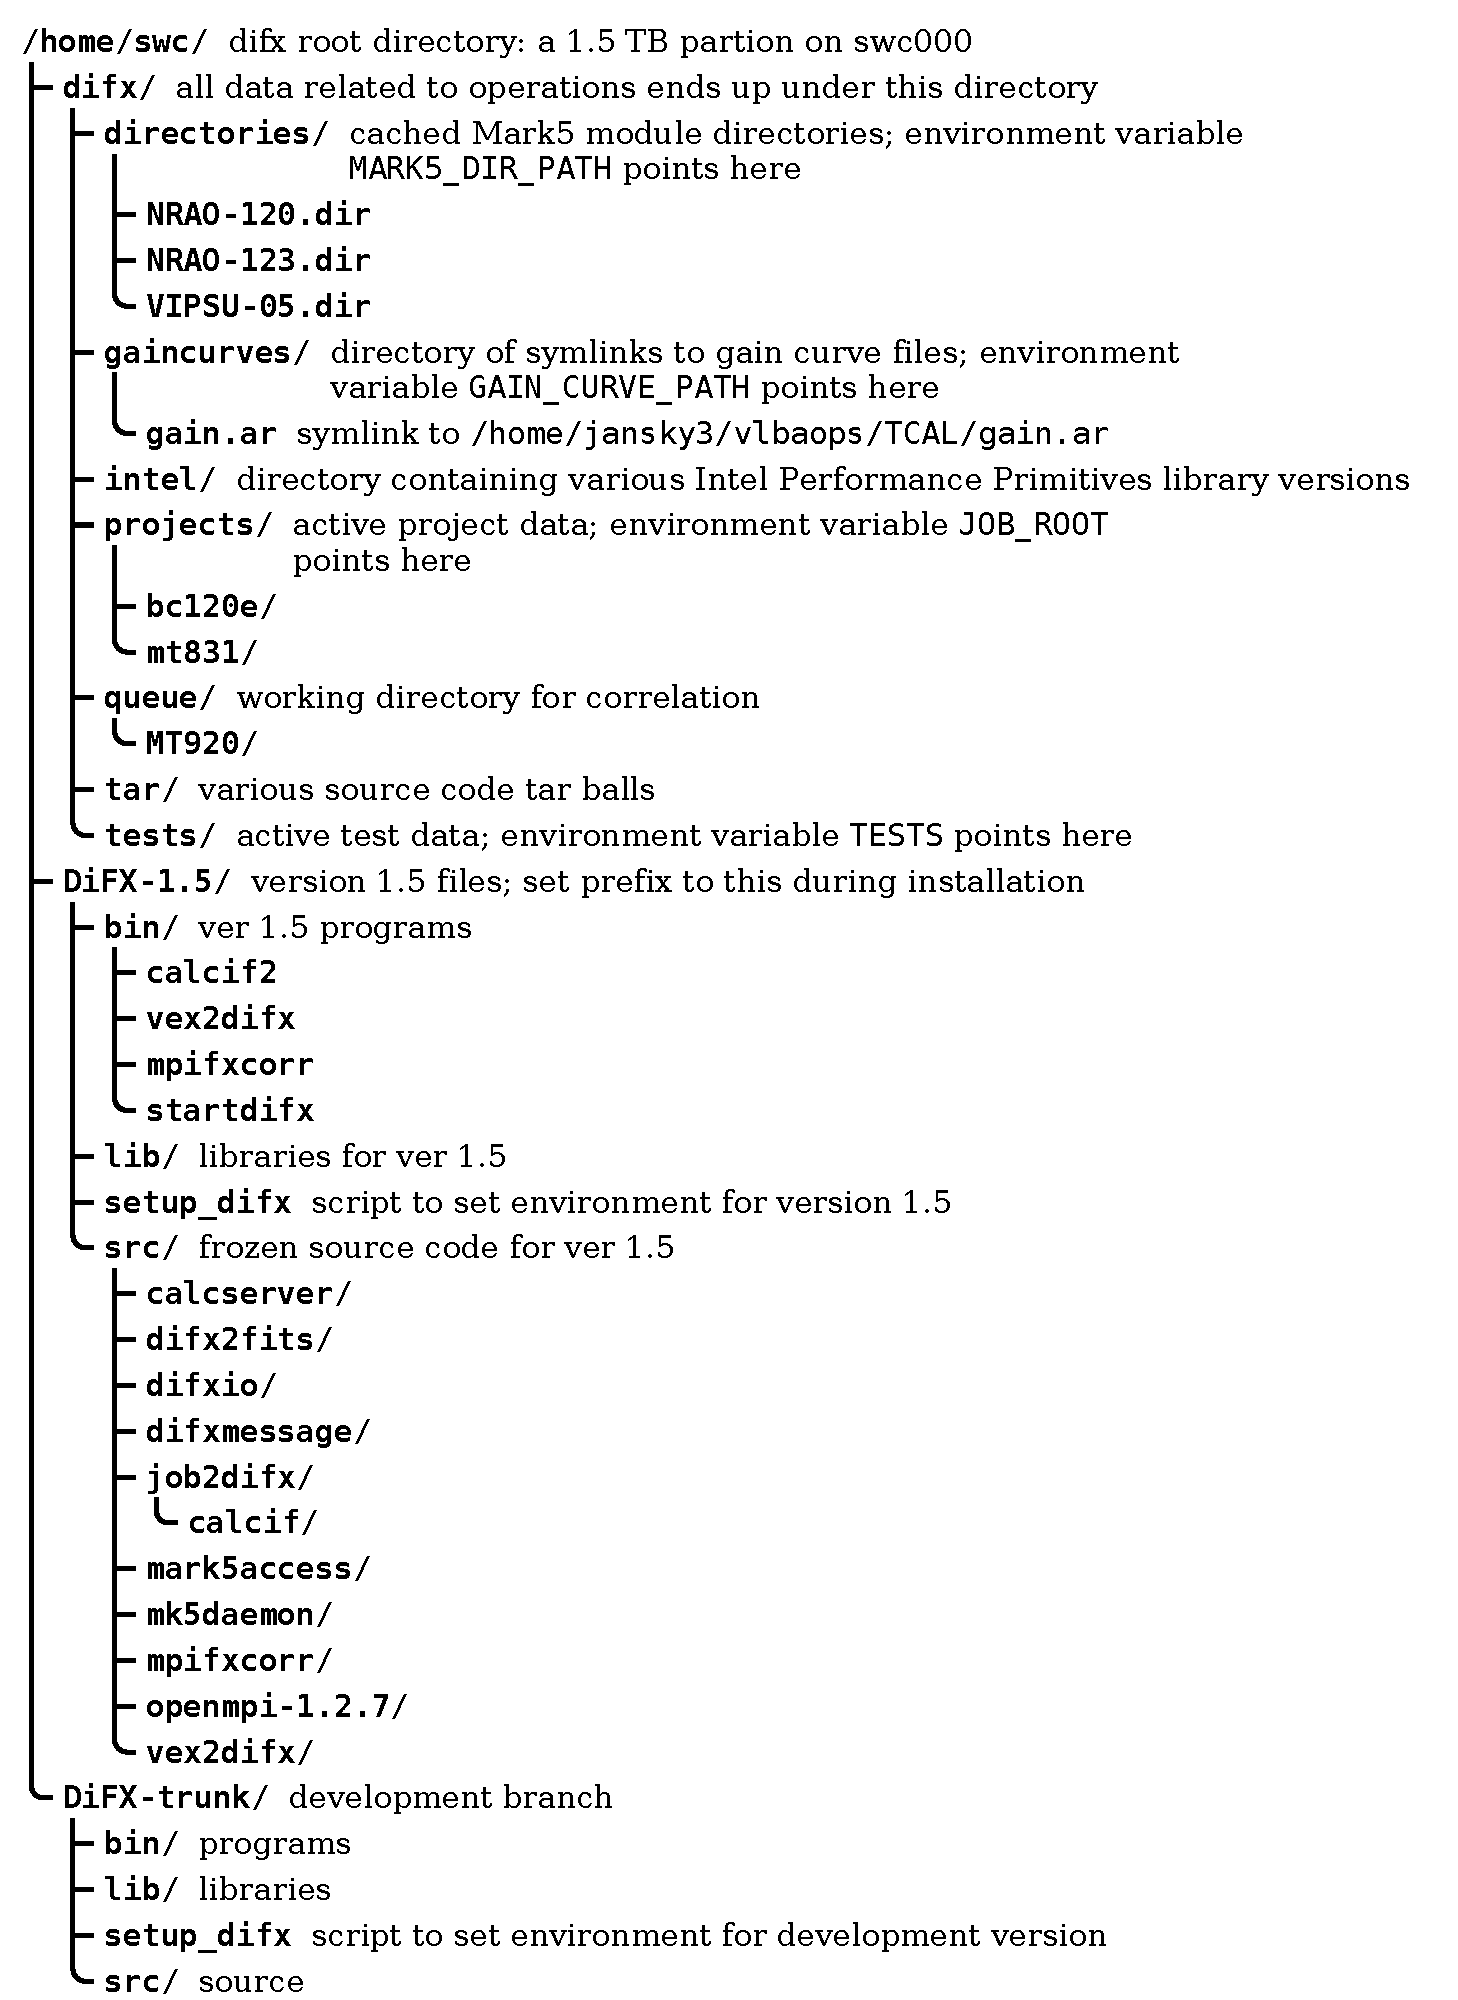
\includegraphics{tree}}
\caption[dirtree]{
{\em The directory structure of the VLBA software correlator.}  
This figure showing the organization of the DiFX directory structure is not comprehensive, but is hopefully complete enough to illustrate the general layout.
For example, only the major top level subdirectories of {\tt DiFX-trunk} are shown.
Entries ending in `/' are themselves directories.
\label{fig:dirtree}
}
\end{center}
\end{figure}

It is highly recommended that one set the {\tt DIFX\_VERSION} environment variable and make sure that for each installed version of DiFX this is set differently.
It may also be desirable to customize this for your correlator.
For example, one may set it to {\tt USNO-DIFX-1.5} .
This string will be stored in intermediate files and the output FITS files and will be able to identify more exactly where the data were correlated.





\section{Running DiFX at the VLBA correlator {\small (VLBA Specific)}} \label{sec:run}

In this section are instructions for using the NRAO adapted DiFX to correlate data that has already been prepared for correlation by the VLBA hardware correlator.
Some aspects of this section may still apply to correlation of other data.
Currently no graphical user interface exists, so these instructions are command line only; these instructions will change when the operator interface is complete.
This section assumes that the software is properly installed and environment variables are set appropriately for use which will be the case for correlator operators.
While there are several steps in performing the software correlation, nothing is too complicated.

Note that this section will see considerable enhancements as experience in running the correlator is gained.

% \subsection{Sharing resources with hardware correlator}
% 
%The Mark5 units attached to the VLBA correlator are used in three different ways for correlation: 1.~An installed module can be played through the VLBA hardware correlator, 2.~The CPU(s) inside the Mark5 unit can be used for software correlator processing, and 3.~An installed module can be played into the software correlator.
%Functions 1 and 2 can be done simultaneously without conflict.  
%Likewise, functions 2 and 3 can also be done simultaneously without conflict.
%Functions 1 and 3 cannot be done at the same time.
%In fact, the software correlator will refuse to use Mark5 units that are currently ``Online'' with regard to the hardware correlator.
%The Mark5 units need to be explicitly set to playback on a particular correlator.  
%See \S\S\ref{sec:take} \& \ref{sec:return} for instructions.
%These two functions cleanly stop and start, respectively, the {\tt Mark5A} program that is needed for the hardware correlator.
%It is only the playback of the Mark5 modules that has any chance of conflict between the software and hardware correlators.
%The hardware correlator can be correlating, idle, in standby, or completely off during software correlation.
%
%\subsubsection{Taking a Mark5 unit} \label{sec:take}
%
%Two actions must be taken to safely transfer a Mark5 unit from serving the hardware to serving the software correlator.
%Here ``safely'' implies no loss of data and no need for an unnecessary reboot; if done properly, no reboots of any computer should be needed.
%First the Mark5 unit must be taken off-line from the hardware correlator {\tt SYSDISCS} screen.
%Multiple units can be taken off-line simultaneously by highlighting multiple units.
%Like usual, units currently assigned to a job cannot be taken off-line.
%Second, the Mark5A program must be stopped on the Mark5 unit(s).
%This can be done with the {\tt mk5take} program (\S\ref{sec:mk5takeprogram}).
%For example, to ``take'' units 8, 9 and 11, one would issue the following command from the shell prompt
%
%\begin{itemize}
%\item[] {\tt mk5take 08 09 11}
%\end{itemize}
%
%Any number of units can be taken off-line at once with {\tt mk5take}.
%Note: if a Mark5 unit is rebooted, {\tt mk5take} will need to be run on that unit again once it comes to life as the {\tt Mark5A} will be automatically started on each reboot (except for units fx01 through fx03 which never run the {\tt Mark5A} program).
%You may need to wait 15 seconds or so after reboot is complete for this to work.
%
%\subsubsection{Returning a Mark5 unit} \label{sec:return}
%
%Once a Mark5 unit is again needed for use with the hardware correlator, it must be returned.
%It is important to make sure the software correlator is not using the particular Mark5 unit for playback before continuing.
%First the Mark5A program must be restarted, which can be done with the {\tt mk5return} program (\S\ref{sec:mk5returnprogram}), e.g.,
%
%\begin{itemize}
%\item[] {\tt mk5return 08 09 11}
%\end{itemize}
%
%Again, any number of Mark5 units can be returned in one call.
%After a few seconds the effectiveness of this can be tested with the {\tt mk5status program}; all units expected to be used for the hardware correlator should be in the READY state.
%Once this is the case, the units can once again be put Online with the {\tt SYSDISCS} screen.
%No reboots should be needed if things go well.



\subsection{Software correlation based on vex files}

With VLBA DiFX version 1.5 comes correlation based on the {\tt .vex} files rather than the hardware correlator jobs scripts.
This new path frees operations from a host of difficult to maintain software, including {\tt cjobgen} and its associated software.
The vex-based correlation was first documented a memo titled ``VLBA-DIFX Operations Plan'' \cite{opsplan}.
Step-by-step instructions describing the process is repeated here.
The particular case being exemplified here is based on the complicated pulsar astrometry project.
Most real-life examples will be simpler, but some may be more complex.
Note that these instructions represent the expected way to proceed, but changes to the software architecture may introduces changes to some of these steps.

It should be kept in mind that all actions performed by the analysts will be {\em pass based} which means one or more jobs at a time.
Rarely will analysts have to worry about individual jobs or FITS files.
The correlator operators on the other hand work entirely on the job basis.
Commands to be issued by the analysts are preceded by an arrow ( $\longrightarrow$ ).
In general, all files written in the processes that follow are readable and writable by everyone in the {\tt vlba\_difx} group.
The exception is data sent to the archive staging area, which is readable and writable only by {\tt e2emgr}.

\begin{enumerate}

\item
First change to the project directory.
Assume that the project is called BX123 and that it was observed in December 2009.

$\longrightarrow$ {\tt cd /home/vlbiobs/astronomy/dec09/bx123}

\item
Extract from the monitor database the Mark5 module logs, clock offsets and rates, and EOPs making a new vex file called {\tt bx123.skd.obs} and a file called {\tt bx123.skd.shelf}.
The original (schedule) vex file that was used during observation is never to be modified.  
In extreme cases, the new vex file being created in this step {\tt bx123.skd.obs} can be hand edited to reflect what actually happened during observation, but doing this should be extremely rare. 
This step locks in the EOP values that will be used for each job made for this project.

$\longrightarrow$ {\tt db2vex bx123.skd}

\item
Next form the template input file for {\tt vex2difx} from the {\tt .oms} file written by {\tt sched} .
This creates {\tt bx123.v2d} .

$\longrightarrow$ {\tt oms2v2d bx123.oms}

\item
For simple experiments it is likely that the {\tt .v2d} file  created in the previous step can be used unmodified.
For this complicated experiment changes will need to be made.
Since this project requires four correlator {\em passes}, this {\tt .v2d} file will need to be copied four times and each one edited to reflect the purpose of the correlator pass.
Sophisticated VLBA users may provide their own set of {\tt .v2d} files that might need light editing before use.

$\longrightarrow$ {\tt cp bx123.v2d clock.v2d}

$\longrightarrow$ {\tt emacs clock.v2d}

\item
VLBA-DiFX {\tt .input} files are generated at this point using {\tt vex2difx}.
By design, {\tt vex2difx} has no options associated with it -- it is entirely configured through the {\tt .v2d} files.
In the case below, the files {\tt clock\_1.input}, {\tt clock\_1.calc}, and {\tt clock\_1.flag} will be created.
This command will also make a file called {\tt clock.joblist} that lists each job created for this correlator pass with a summary of the job properties, such as start and stop times and number of stations.

$\longrightarrow$ {\tt vex2difx clock.v2d}

\item
If the correlator jobs created above are deemed ready to run, they are sent to the correlator queue.
In this process three things will occur: 1. {\tt CALC} will be run to generate the correlator delay models needed for correlation, 2. the {\tt .input} files generated by {\tt vex2difx} will be copied to the software correlator run directory, and 3. the VLBA database will be told that the jobs are ready.
At this time, a priority can be set to the jobs being sent to the correlator, making them appear at the top of the queue.
Otherwise the jobs in the queue will appear in observe time order.
In the example below, the option {\tt -p 1} indicates that this job should run with elevated priority.
Supplying {\tt clock} with no prefix implies queuing all the jobs in the clock pass.
Individual jobs could be queued by specifying a list of {\tt .input} files.

$\longrightarrow$ {\tt difxqueue -p 1 add clock}

\item
When the jobs are complete, which can be determined with {\tt difxqueue} using the {\tt list} action, the correlator output is converted to FITS format.
Data ``sniffing'' happens automatically during this step.
The command to do this will ensure that all of the jobs in the pass have been successfully correlated.
Note that the number of FITS files created is not necessarily the same as the number of correlator jobs.
A file called {\tt clock.fitslist} will be generated in this step that lists all of the fits files that are part of this correlator pass including for each FITS file a list of the jobs that contributed to that FITS file. 
The program {\tt makefits} will use program {\tt difx2fits} to do the actual conversion.


$\longrightarrow$ {\tt makefits clock.joblist}

\item
The sniffer output files are at this point inspected.
Program {\tt difxsniff} is run to produce plots which are identical to those produced by sniffer today. 
Multiple reference antennas (in this example, Los Alamos and Kitt Peak) can be provided at the same time.
Sniffer plots and the data that is used to generate them will be placed in a sub-directory of the project directory called {\tt sniffer/clock} for a pass called ``clock''.

$\longrightarrow$ {\tt difxsniff LA KP clock.fitslist}

$\longrightarrow$ {\tt gv sniffer/clock/apdfile.ps}

\item
If the FITS files are deemed acceptable, they are entered into the VLBA data archive.

$\longrightarrow$ {\tt difxarch clock.fitslist}

\item
Finally, once data has been archived, the intermediate files should be removed from the head node:

$\longrightarrow$ {\tt difxclean bx123}

Note that this final step is needed only after the entire project is ready for releasing and should not be done every time between completion of job passes.

\end{enumerate}



%\subsection{Software correlation based on FXCORR job files}
%
%The initial deployment of the software correlator at the VLBA relied on conversion of hardware correlator (FXCORR) job scripts ({\tt .fx} files) to DiFX {\tt .input} files.
%This procedure is being phased out in favor of correlation based on {\tt .vex} files; the instructions for correlation based on this earlier pathway is explained below mainly for historical reference.
%This pathway into DiFX may still be useful in some circumstances.
%The procedure below does not go into any detail about what is actually happening at each step, please find details in other sections of this manual.
%Only steps \ref{item:take} though \ref{item:done} below require the correlator-specific hardware so the pre- and post- correlation steps could all be run by the analysts rather than operators.
%In the example that follows, project BM264 segment G will be correlated:
%\begin{enumerate}
%\item Log into the head node as user: {\tt ssh -l difx \$DIFX\_HEAD\_NODE}
%\item Change directories to the job root directory: {\tt cd \$JOB\_ROOT}
%\item Copy the job scripts and monitor data over: {\tt getjobs bm264g} (\S\ref{sec:getjobs})
%\item Enter the project directory: {\tt cd bm264g}
%\item At this time it would be convenient to open another terminal, log into {\tt \$DIFX\_HEAD\_NODE} as difx, and change to the {\tt \$JOB\_ROOT} directory so that it is easy to monitor the progress in one window while running the correlation in the other.
%\item Generate the DiFX input files: {\tt job2difx *.fx} (\S\ref{sec:job2difx}).
%\item Look over the list of jobs to be done: {\tt joblist} (\S\ref{sec:joblist}). \label{item:jl}
%\item Determine which modules are needed, either by looking at the {\tt .fx} files or with the use of {\tt jobdisks} (\S\ref{sec:jobdisks}).
%Install these modules into Mark5 units, making sure not to put two modules that are needed by the same job into the same unit.
%\item Off-line the units using the hardware correlator {\tt SYSDISCS} screen and ``take'' them (\S\ref{sec:take}). \label{item:take}
%Note that if no hardware correlation is to occur it is okay to ``take'' all of the Mark5 units for convenience.
%\item \label{item:sd} At this point one could start the correlation of all the jobs with a single command: {\tt startdifx *.input} (\S\ref{sec:startdifx}), but it is recommended to start just one job first to make sure things are working: {e.g. \tt startdifx job1240.000.input} .
%\item When output stops and the command prompt is given back, the processing is either done or something failed.
%If a job is encountered that requires a module that is not mounted, processing will stop with a warning that the module could not be found.
%At this point, you should load the desired module and again type {\tt startdifx *.input} to continue processing. 
%\item When done, return the Mark5 units if they are needed by the hardware correlator (\S\ref{sec:return}). \label{item:done}
%\item Generate fits files for all correlated jobs: {\tt difx2fits -d} (\S\ref{sec:difx2fits}). \label{item:end}
%\end{enumerate}
%
%If a job is encountered and a required module for that job is not installed in a Mark5 unit that has been ``taken'', the correlation process will stop.
%The needed module will be listed in an error report, or can be identified using the {\tt jobdisks} (\S\ref{sec:jobdisks}) program.
%
%
%\subsection{Common failure modes}
%
%Here is a list of some common failure modes and some hints to identifying and solving them.
%In general, it is often useful to look at the correlator log.
%The DOI will keep in a buffer the running log from the recent correlation sessions.
%Copies of all logs are stored in {\tt \$DIFX\_QUEUE/}{\em project} .
%Note that {\em project} in this context includes the segment code and is completely capitalized.

\subsubsection{Directory contains undecoded scans}

Occasionally a message of the form {\tt Module }{\em module} {\tt directory contains undecoded scans!} will appear.
This means that one or more scans for the module named {\em module} was not properly read or decoded.
This should first be verified by examining the module directory file, called {\tt \$MARK5\_DIR\_PATH/}{\em module}{\tt .dir} .
This examination is best done with program {\tt checkdir} which looks for a number of possible abnormalities.
Rows where the eleventh column contains a negative number are scans that were not decoded properly.
A known problem occasionally causes many consecutive scans at the end to be improperly read and thus undecoded.  
If this is the case, rename the existing directory file and try reacquiring the directory.
Usually it will start working immediately.

If one or a small number scans repeatedly cannot be decoded, the scan may be corrupted for some reason.
In this case, simply delete the row(s) from the directory file and then decrement the number following the module name on the first line of the file by the number of scans deleted; this count of the number of scans listed in the file must remain accurate.
This operation will cause the correlator to skip over these affected scans and data will be lost, so use appropriate judgement in these cases.

\subsubsection{Directory read fails on partial module}

Modules containing less than 8 working disks can be problematic.  
It is suggested that modules of this type have their directories read
preemptively using a special command:

\noindent
$\longrightarrow$ {\tt mk5control safedirA 12}

\noindent
which is the command to {\em safely} read the directory of the module in bank {\tt A} of {\tt mark5fx12}.

\subsubsection{Mark5 unit hangs while reading directory}

Typically the first thing one should do if a hang occurs is to try again.
For directory reading this can be attempted with the {\tt mk5control} program.
For instance, if the module in bank {\tt A} of {\tt mark5fx12} hangs during the directory read, stop the correlation process with the DOI or via {\tt stopmpifxcorr} and then issue:

\noindent
$\longrightarrow$ {\tt mk5control getdirA 12}

\noindent
If this also fails, or never starts, reboot the unit via the DOI or

\noindent
$\longrightarrow$ {\tt mk5control reboot 12}

\noindent
or

\noindent
$\longrightarrow$ {\tt ssh 12 /sbin/reboot} if it really refuses to reboot.

Once the unit comes back, try retrieving the directory again.

\subsubsection{Mark5 directory reading fails partway through}

When the GUI button GetDir fails, the program {\tt mk5dir} can be used directly to read a module directory.

Things to try first:
\begin{enumerate}
\item Log into the fx unit and run {\tt vsn} to look for obvious module problems
\item Move the module
\item Erase (or move/rename) the preexisting directory file
\item Reboot the correlator Mark5 unit
\end{enumerate}

When GetDir fails or crashes the Mark5 unit, it is likely because there are one or more spots on the module that can't be read.
Using {\tt mk5dir}, you can read most of the directory while skipping any problematic scans.

The {\tt mk5dir} program will work on both Mark5A and Mark5C modules.
It is best to put them, respectively, in SDK 8 and 9 units.
As with most utilities, typing {\tt mk5dir} by itself will print help information.

The output directory will be named the usual {\em vsn}.dir and will overwrite
any existing file of that name. It will be written to {\tt \$MARK5\_DIR\_PATH}, which is the same place to which GetDir writes directories.

The relevant options in this case are:

\begin{itemize}
\item {\tt -f} (force a directory read even if a file already exists)
\item {\tt -v} (be verbose)
\item {\tt -e} {\em scan number} (stop reading the directory at a certain scan number)
\item {\tt -b} {\em scan number} (begin reading the directory at a certain scan number)
\end{itemize}

The scan numbering is worth noting.
The command line options {\tt -e} and {\tt -b} number the scans starting at 1 (the first scan is 1).
But the on-screen output of {\tt mk5dir} will begin with a scan numbered 0.

The first step is to read as much of the directory before the first problem scan.

\begin{enumerate}
\item Log in to the fx unit
\item Run {\tt vsn} {\em bank} to get an overview of the health of the module
\item Run {\tt mk5dir -f -v} {\em bank}
\end{enumerate}

As it reads each scan, it will print a line indicating its progress.

\noindent
{\tt 0/228 -> 3 Decoded} \\
{\tt 1/228 -> 3 Decoded} 

etc \ldots

The first number is the scan it just decoded and the second number is the total number of scans on the module.
The ``3'' is related to the data format and should be 3 for Mark5C at all VLBA sites.
VLA modules will show ``4''.
Legacy VLBA and foreign stations may show other numbers.
The ``Decoded'' indicates success, as opposed to something like ``XLR Read Error''.

Presumably, it will fail at some point.
When it fails it probably won't write an output directory file.
Note which scan it failed to read. Remember that scan $x/228$ is actually the $x$+1$^{\mathrm th}$ scan because it started counting at zero.
You may have to reboot the fx unit at this point.

Now run {\tt mk5dir} again, this time stopping one scan previous to the one where it died last time.

\begin{enumerate}
\item Run {\tt vsn} {\em bank} (whether you had to reboot or not, checking the module with {\tt vsn} is probably a good idea)
\item Run {\tt mk5dir -f -v -e} $x$ {\em bank} ({\tt mk5dir} will stop once it has read $x$ scans)
\item Rename the output file so it doesn't get overwritten.
\end{enumerate}

Now we can skip past the bad parts and read the rest of the directory.

\begin{enumerate}
\item Run {\tt mk5dir -f -v -b} $x$+2 {\em bank} ({\tt mk5dir} will start with the scan after the one it originally failed on)
\end{enumerate}

If it fails, reboot as necessary, run vsn again, and try starting with scan $x$+3 instead.
Keep incrementing the start scan until it works; sometimes it might be faster to try a bigger jump, and on success work backwards to find where failing starts.
Eventually, you will have skipped past the bad scans and read the rest of the directory.
There are likely to only be one or two bad scans, so this step should actually be fairly simple.

Now you will have two directory files, the renamed file with the first $x$ scans, and the second file with all the scans after the bad scan(s).
Each file will also have entries for the scans that weren't read by that particular invocation of {\tt mk5dir}, and these lines need to be deleted.
Then using your preference of linux commands and/or text editor, combine the two files in the appropriate order.
Make sure there is a single header line at the top which lists the correct number of scans.

If there are nonsequential bad scans you will have to concatenate three or more files, but the steps remain the same.


\subsubsection{Mark5 unit hung} %FIXME
Unfortunately, there are still some instabilities with Mark5 units that result in various kinds of hangs; some units appear more sensitive than others.
Often a failed Mark5 can be identified with the last few lines of error messages output from {\tt mpifxcorr}.
To verify, first attempt to {\tt ssh} into that unit.
If that is successful, try watching the output of {\tt cpumon} and {\tt mk5mon} (or the equivalent from the {\tt DOI}).
If no updates come from {\tt cpumon} then it is likely that the computer has seized and requires a hard reboot.
Otherwise if {\tt mk5mon} shows no updates, the problem is likely with the Streamstor card and/or disk module.
If logging into the Mark5 unit works, try resetting the Streamstor card with:

{\tt mk5control reset } {\it unitNumber}

\noindent where {\it unitNumber} is, for example, 07 for mark5fx07 or 23 for mark5fx23.
The Mark5 state shown in {\tt mk5mon} should change to ``Resetting''.
If it does not, then it is likely a reboot is needed.

If none of the above works, try rebooting the particular Mark5 unit and starting over.
Note: as currently configured, a Mark5 unit will restart the {\tt Mark5A} upon boot, so you will need to use {\tt mk5take} to stop that before attempting software correlation on that unit again.  
Make sure to give the Mark5 unit enough time to initialize the {\tt Mark5A} program before running {\tt mk5take} (i.e., wait for module lights to cycle).

A possibly more reliable way to identify a hung Mark5 unit is to start a new instance of {\tt mk5mon} (\S\ref{sec:mk5mon}) in a terminal and issue the following command: 

{\tt mk5control getvsn mark5}

\noindent A hung Mark5 will not show up in the list of units.

\subsubsection{Module moved}
If a required module has been removed or moved since {\tt genmachines} has run, {\tt mpifxcorr} will not be able to correlate.
In this case DiFX will fail, spitting out a substantial amount of debug information.
You can try again by running {\tt genmachines} {\em baseFilename}{\tt .input} to force the recreation of the {\tt .machines} file.
If this program fails, it will report an error that may aid in diagnostics.
Note that this scenario will not happen if the Difx Operator Interface or {\tt startdifx} (\S\ref{sec:startdifx}) is used to run the correlator.

\subsection{Correlating data files} \label{sec:datafiles}

The operating instructions up to this point have focused on correlation directly off Mark5 modules.
Correlation off files is also supported, as is a mixed mode where files and modules are correlated together.
The scripts described in this document don't (to date) make correlation of files easy, but it is possible to do so by hand editing files.
It is expected that enhancements to the scripts will make correlation from files much easier in future versions of DiFX.
Two files will need manipulation: {\tt .input} and {\tt .machines}.
In the {\tt .input} file, every entry in the {\tt DATASTREAM} table that corresponds to a disk file needs the {\tt DATA SOURCE} value changed from {\tt MODULE} to {\tt FILE}.
The {\tt .machines} file will likely have to be constructed completely by hand.
See \S\ref{sec:machines} for a detailed description of the format of that file.
Note that it is no longer necessary for the data files to be visible to all cluster computers -- they can reside on local drives that are not exported, including USB or Firewire drives, but this requires that the datastream nodes listed in the {\tt .machines} file be in the order in which the antennas are listed in the {\tt .input} file.

\noindent 
{\em Note:} you must use the {\tt -n} option to {\tt startdifx} when starting the correlation or the hand-edited {\tt .machines} file will be overwritten.


\subsection{The VLBA database}

Many of the existing VLBA tools (such as the Observation Management System (OMS), {\tt mon2db}, {\tt cjobgen}, and others) make use of an Oracle database for persistent storage of various information related to projects that use either the VLBA antennas or correlator.
Many aspects of VLBA-DiFX are not a good match for the existing database tables; adapting the existing tables to work nicely with VLBA-DiFX will be disruptive and have implications for much existing code, including software that will not be needed once FXCORR is shut down.
The proposed solution to this dilemma is to use a parallel set of database tables for correlation and archiving when using VLBA-DiFX.
The use of existing software for generation of FXCORR jobs will continue unchanged.
For projects to be correlated using VLBA-DiFX, {\tt OMS} will still be used for observation preparation tasks, but will not be used in preparation of correlation or anything that occurs beyond that in the project's life cycle.  Instead, {\tt vex2difx} will be used to generate jobs, {\tt difxqueue} will be used in lieu of {\tt OMS} to stage correlator jobs, and {\tt difxarch} will be used in the archiving of data.
The queuing tool {\tt difxqueue} will be used to display the state of the VLBA-DiFX job queue as well as populate it.
The new tools will access three new database tables: DIFXQUEUE and DIFXLOG; the contents of these tables is shown in Tables\,\ref{tab:difxqueue}\,\&\,\ref{tab:difxlog}.

\begin{table}[h]
\vspace{2mm}
\begin{center}
\renewcommand{\tabcolsep}{1.4mm}
\begin{tabular}{lll}
\hline
\hline
   \multicolumn{1}{l}{Column}
 & \multicolumn{1}{l}{Type}
 & \multicolumn{1}{l}{Comments}
\\
\hline
PROPOSAL	& VARCHAR2(10)	& The proposal code \\
SEGMENT		& VARCHAR2(2)	& Segment (epoch) of proposal, or blank \\
JOB\_PASS	& VARCHAR2(32)	& Name of correlator pass (e.g. ``geodesy'') \\
JOB\_NUMBER	& INT		& Number of job in the pass \\
PRIORITY	& INT		& Number indicating the priority of the job in the queue \\
		&		& 1 is highest \\
JOB\_START	& DATE		& Observe time of job start \\
JOB\_STOP	& DATE		& Observe time of job stop \\
SPEEDUP         & FLOAT         & Estimated speed-up factor for job \\
INPUT\_FILE	& VARCHAR2(512)	& Full path of the VLBA-DiFX input file \\
STATUS		& VARCHAR2(32)	& Status of the job, perhaps ``QUEUED'', ``KILLED'', \\
		&		& ``RUNNING'', ''FAILED'', ''UNKNOWN'' or ``COMPLETE'' \\
NUM\_ANT	& INT		& Number of antennas in the job \\
\hline
\end{tabular}
\end{center}
\caption{
The DIFXQUEUE database table.
This table is based on the FXQUEUE table currently used by {\tt OMS}.
Entries to this table will be initially made by {\tt difxqueue}.
The STATUS field will be automatically updated as appropriate during correlation.
\label{tab:difxqueue}}
\end{table}

\begin{table}[h]
\vspace{2mm}
\begin{center}
\renewcommand{\tabcolsep}{1.4mm}
\begin{tabular}{lll}
\hline
\hline
   \multicolumn{1}{l}{Column}
 & \multicolumn{1}{l}{Type}
 & \multicolumn{1}{l}{Comments}
\\
\hline
PROPOSAL	& VARCHAR2(10)	& The proposal code \\
SEGMENT		& VARCHAR2(2)	& Segment (epoch) of proposal, or blank \\
JOB\_PASS	& VARCHAR2(32)	& Name of correlator pass (e.g. ``geodesy'') \\
JOB\_NUMBER	& INT		& Number of job in the pass \\
CORR\_START	& DATE		& Start time/date of correlation \\
CORR\_STOP	& DATE		& Stop time/date of correlation \\
SPEEDUP         & FLOAT         & Measured speed-up factor \\
INPUT\_FILE     & VARCHAR2(512) & File name of .input file \\
OUTPUT\_FILE	& VARCHAR2(512)	& File name of correlator output \\
OUTPUT\_SIZE	& INT		& Size (in $10^6$\,bytes) of correlator output \\
CORR\_STATUS	& VARCHAR2(32)	& Status of correlation, typically ``COMPLETED'' \\
\hline
\end{tabular}
\end{center}
\caption{
The DIFXLOG database table.  This table is based on the FXLOG table currently used by {\tt OMS}.
A row will be written to this table after each successful correlation by the DiFX Operator Interface.
\label{tab:difxlog}}
\end{table}

\subsection{Archiving} \label{sec:archive}

Archiving of VLBA-DiFX data will be done on a per-pass basis.
All {\tt .FITS} files associated with a single correlator pass will be archived together.
A particular staging directory for VLBA-DiFX data has been set up.
Populating the archive amounts to first copying the files to be archived to this directory making sure that the first character of the file name is ``.''.
Once the entire file is transferred this file is renamed without the leading period.
This system is the standard way to populate the Next Generation Archive System (NGAS) \cite{ngas} without potential for an incompletely copied file to be archived.
The file names will be composed only of alpha-numeric characters and ``.'' and ``\_''.
These characters have no special meaning in any relevant software, including http, XML, bash/Linux command lines, the Oracle database parser, etc.  File names will have the following format:

\vspace{5pt}

{\tt VLBA\_}{\em projectCode}{\tt \_}{\em passName}{\tt \_}{\em fileNum}{\tt \_}{\em corrDate}{\tt T}{\em corrTime}{\tt .idifits}

\vspace{5pt}

\noindent
where the italicized fields, which themselves will be limited to alphanumeric characters, are as follows:

\begin{center}
\begin{tabular}{lll}
\hline
\hline
Field & Type & Comment \\
\hline
{\em projectCode}	& string		& Project code, including segment if appropriate \\
{\em passName}		& string		& Name of the pass, as set in the {\tt .v2d} file \\
{\em fileNum}		& integer		& FITS file sequence number within pass \\
{\em corrDate}		& date ({\em yymmdd})	& Date corresponding to correlation completion \\
{\em corrTime}		& time ({\em hhmmss})	& Time corresponding to correlation completion \\
\hline
\end{tabular}
\end{center}

\noindent
Parameter {\em fileNum} is the sequence number of the created {\tt .FITS} file which may or may not have a direct correspondence with the job sequence number within the correlator pass.
An example archive file name relevant to the sample project used in this memo may be:

\vspace{5pt}

{\tt VLBA\_BX123\_clock\_1\_091223T032133.idifits}

\vspace{5pt}

\noindent
All files produced for a given pass will be placed in a single directory, 

\vspace{5pt}

{\tt \$DIFX\_ARCHIVE\_ROOT/}{\em projectCode}{\tt /}{\em passName}

\vspace{5pt}

\noindent
where {\tt DIFX\_ARCHIVE\_ROOT/} is an environment variable pointing to the head of the archive staging area for VLBA-DiFX.
During the transfer to the archive, the {\em projectCode} portion of the directory tree will begin with a period that is to be renamed once all files are completely copied.
This will allow the archive loader to logically group together all the files of the pass.
If needed, an index file listing the association of archive {\tt .FITS} files and correlator jobs can also be placed in this directory.
In order to ensure the atomic nature of correlator passes in the archive, the renaming of the copied files from the temporary versions starting with ``.'' will not occur until all archive files are transferred.
The {\tt .fitslist} file produced by {\tt difx2fits} would serve this purpose.
An archive loader will periodically (initially about every 30 minutes, but perhaps later with much shorter intervals)\ look for new files in the archive staging area to store.
The archive data will be available moments later for users wanting to download the data.

\subsection{Ownership and permissions of files} \label{sec:permissions}

This section describes how the different user accounts interact within the DiFX correlation process.
This is VLBA operations specific.
No fewer than 4 user accounts are used in the life cycle of a DiFX project:

\begin{itemize}

\item {\it analysts}: 
The analysts account is used to prepare the {\tt .input} and other files used to run DiFX.
These files retain {\em analysts} ownership in the {\tt /home/vlbiobs/astronomy} area and while queued.

\item {\it root}:
The root account owns the {\tt mk5daemon} processes that run on each of the Mark5 and software correlator computers.

\item {\it difx}:
User account {\it difx} is used to actually run {\tt mpifxcorr} (and {\tt difxlog}) during correlation.
This is important, as the {\it difx} account has all of the proper environment variables set up.
The DiFX Operator Interface may also be run as user {\it difx}.

\item {\it e2emgr}:
The data archive requires that the files staged for entry into the archive be given {\it e2emgr} ownership.
This is accomplished with the prgram {\tt e2ecopy} which runs with root priviledges and hence can change its userid to {\it e2emgr} as needed.

\end{itemize}

By default, all files will have owner and group read/write permission and global read permission.

\subsection{Copying baseband data} \label{sec:datacopy}

Some users wish to perform their own analysis on baseband VLBI data.
This section describes the procedure for copying data and ends with guidelines that should be sent to each user requesting data to be copied.
The guidelines are there to streamline the process and to minimize the change of problems.

\subsubsection{Performing the data copy}

{\em FIXME : write me!}

\subsubsection{Guidelines to users}

Users wishing to retain a copy of the baseband data should make sure to
conform to the following guidelines.  Please note that many of the
instructions below are there to ensure that root access is not required in
the copying of the data.  If root access is needed as a result of failure to
comply, a delay in the copying will be incurred.

\begin{enumerate}
\item Arrangement for data copy should be made prior to observing.

\item The external disk must have a working USB2 connector for data transfer.
We specifically do not support Firewire at this time.  
We do not support power-over-USB drives.

\item Each disk should have a sticker label attached with the owner's name, institution, phone number, shipping address and email.  
The project code should be clearly marked as well.  
If multiple disks are shipped, each should have a unique serial number clearly labeled on the disk.

\item The external disk must be preformatted with a standard Linux filesystem (ext2 or ext3).
It is preferred that the options {\tt -m 0 -T largefile4} are used with {\tt mke2fs} and it is also suggusted that the {\tt -L} option is used to specify a volume name/number that matches the labelled serial number.

\item It is the user's responsibility to ensure that sufficient post-formatted capacity is available on the disks.

\item A world-writable root-level directory with the name of each project to be copied should be made.
The directory name should contain only uppercase letters and numbers.

\item The disk should be empty upon delivery.  
NRAO will not be responsible for data that is deleted.  
The root-level directory(s) mentioned above should be the only exception(s).

\item Include the power transformer/cable and USB cable with the disk.  
It is recommended that owner labels be attached to each of these.

\item Note to foreign users: please ensure that the power supply has either a NEMA 1-15 / Type~A ungrounded power connector or a NEMA 5-15 / Type~B grounded power connector and that the power supply works on 110V/60Hz.
If this is accomplished using an adapter, it must be included in the box with the disk.

\item Foreign users will be responsible for customs charges and are encouraged to contact NRAO well in advance of any shipment to minimize cost.

\end{enumerate}




\subsection{Some comments on channels}

This section discusses the accountability of channel identification through the entire DiFX system.
While much of this discussion will not be of use outside NRAO, the terminology discussed here might help explain other portions of this document.  
The subject of this section is baseband channels, not individual frequency channels that the correlator produces from
the baseband channels.

Baseband channels are individual digital data streams containing a time-series of sampled voltages representing data from a particular portion of the spectrum from one polarization.
Each baseband channel is assigned a recorder channel number.
For a given baseband data format (i.e., VLBA, Mark4, Mark5B, ...) a particular recorder channel number is assigned to a fixed number of tracks or bitstreams.
This mapping is contained in the {\tt track} row in the {\tt format} table of the {\tt .fx} job script and can be different for each antenna.
This mapping is also reflected in the {\tt .input} file in the {\tt datastream} table.

DiFX correlates baseband channels from multiple antennas to produce visibilities.
From each correlated baseline, one or two basebands from one telescope will be correlated against one or two basebands of another, resulting in up to four products for a particular sub-band.
This is to allow full polarization correlation.
Each sub-band (called an IF in AIPS) is given a sub-band number; in general 1 or 2 recorder channels map to each sub-band.
Note that an observation can simultaneously observe some sub-bands consisting of only one baseband and some with two basebands.
In cases such as this the matrix containing the visibility products on a particular baseline will be large enough in each dimension (i.e., polarization product, sub-band) to contain all of the results, even if this consumes more storage than necessary; flags are written that invalidate portions of the visibility matrix that are not produced by the correlator.  


\section{DiFX and pulsars} \label{sec:pulsars}


%TODO:
%tempo2 example (Jan)
%profile2binconfig
%  - 2 modes
%  - single input file allowed
%makeemptybinconfig (JW -- to be added)



DiFX supports four pulsar processing modes:

\begin{itemize}

\item \label{psrmode:binarygate} {\bf Binary Gating}  
A simple on-off pulse accumulation window can be specified with an ``on'' phase and an ``off'' phase.
This can be used to boost the signal to noise ratio of pulsar observations by a factor of typically 3 to 6 and can also be used to search for off-pulse emission.

\item \label{psrmode:matchedgate} {\bf Matched-filter Gating}
If the pulse profile at the observation frequency is well understood and the pulse phase is very well predicted by the provided pulse ephemeris, additional signal to noise over binary gating can be attained by appropriately scaling correlation coefficients as a function of pulse phase.
Depending on the pulse shape, addition gains by a factor of up to 1.5 in sensitivity over binary gating are realizable.

\item \label{psrmode:bin} {\bf Pulsar Binning}
Pulsar {\em binning} is supported within DiFX.
This entails generating a separate visibility spectrum for each requested range of pulse phase.
There are no explicit limits to the number of pulse phase bins that are supported, however, data rates can become increasingly large.
Currently AIPS does not support databases with multiple phase bins. 
Until there is proper post-processing support for pulsar binning, a separate FITS file will be produced for each pulsar phase bin.

\item \label{psrmode:profile} {\bf Profile Mode}
Profile mode is very different than the other three as it generates autocorrelations only that are used to determine the pulse shape and phase rather than generating cross correlations.
This mode is enabled by placing {\tt mode=profile} in the global scope of the {\tt .v2d} file (conventionally near the top).
The {\tt .v2d} file can enable as many antennas as desired (they will be averaged, so if you have a single large antenna it is probably best to include only that one), but can only operate on one source at a time.
The output of {\tt mpifxcorr} can be turned into an ASCII profile with {\tt difx2profile}.
This profile can then be given to {\tt profile2binconfig.py} to generate the {\tt .binconfig} file that is used by the other three pulsar modes.
There is some evidence that after about 10 minutes of integration the signal to noise ratio of the resultant profile stops growing.
This remains to be fully understood.
It could be that increasing the integration time helps; there is no reason not to use quite large integration times in this mode.

\end{itemize}

In all cases the observer will be responsible for providing a pulsar
spin ephemeris, and in all cases this ephemeris must provide an accurate
description of the pulsar's rotation over the observation duration (the pulsar 
phase must ont drift substantially with time).  If gating is to be applied then 
the ephemeris must be additionally be capable
of pedicting the absolute rotation phase of the pulsar.
Enabling pulsar modes incurs a minimum correlation-time penalty of
about 50\%.  High output data rates (computed from time resolution,
number of spectral channels, and number of pulsar bins) may require 
greater correlator resourse allocations.
The details of pulsar observing, including practical details of using
the pulsar modes and limitations imposed by operations, 
are documented at \url{http://library.nrao.edu/public/memos/vlba/up/VLBASU_32.pdf}.

\subsection{Pulse ephemeris}

The use of any pulsar mode requires a pulse ephemeris to be provided by the astronomer.  
This is a table of one or more polynomial entries, each of which evaluates the pulsar's rotation phase over an interval of typically a few hours.
The classic pulsar program {\tt Tempo} can be used to produce the polynomials required \cite{tempo}.
The pulse phase must be evaluated at the Earth center which is usually specified in {\tt tempo} by station code 0 (zero).
Many pulsars exhibit a great degree of timing noise and hence the prediction of absolute pulse phase may require updated timing observations.
When submitting the polynomial for use at the VLBA correlator, please adhere to the following naming convention: {\em experiment}{\tt -}{\em pulsar}{\tt .polyco} , e.g., {\tt BB118A-B0950+08.polyco} .
Instructions for generating the polynomial file are beyond the scope of this document.

Each {\tt .polyco} contains one or more polynomials along with metadata; an example {\tt .polyco} file that is known to work with DiFX is shown immediately below:
\begin{verbatim}
1913+16     6-MAY-15   90748.00   57148.38041666690           168.742789 -0.722 -6.720
   6095250832.610975   16.940537786201    0   30   15  1408.000 0.7785   3.0960
  0.18914380470191894D-06  0.26835472311898462D+00 -0.10670985785738883D-02
 -0.85567503020416261D-05 -0.55633960226391698D-07 -0.37190642692987219D-09
 -0.58920583351397697D-12 -0.27311855964499407D-12 -0.21723579215912174D-13
  0.11968684344685061D-14  0.92517174535020731D-16 -0.28179552068141251D-17
 -0.18403230317431974D-18  0.25241984130137833D-20  0.13743173681516959D-21
\end{verbatim}
\noindent
A description of the file format is available at \url{http://tempo.sourceforge.net/ref_man_sections/tz-polyco.txt}.
Currently {\tt tempo} (version 1) is well supported and {\tt tempo2} is only supported in {\tt tempo1} compatibility mode.
Eventual support for the {\tt tempo2} {\em predictors} will be added.
All ephemerides must be made for the virtual Earth Center observatory (i.e., XYZ coordinates 0,0,0, usually observatory code 0; DiFX versions prior to 2.5 would not accept any non-numeric code even though they are legal).
Any reference frequency can be specified as the correlator takes dispersion into consideration.

Note that although {\tt tempo} version 2 can produce usable {\tt .polyco} files experience has shown that version 1 has fewer failure modes.

\subsection{Bin configuration file}

All three pulsar modes also require the preparation of a {\tt .binconfig} file by the astronomer.
The contents of this file determine which of the three pulsar modes is being used.
Three pieces of information are contained within this file: the pulsar ephemeris (polyco) files to apply, definitions of the pulsar bins, and a boolean flag that determines whether the bins are weighted and added within the correlator.
The file consists of a set of keywords (including a colon at the end) that must be space padded to fill the first 20 columns of the file and the values to assign
to these keywords that start at column 21.
The file is case sensitive.
The pulsar bins each consist of a ending phase and a weight; each bin is implicitly assumed to start when the previous ends and the first bin starts at the end phase of the last.
The phases are represented by a value between 0 and 1 and each successive bin must have a larger ending phase than the previous.
Examples for each of the three pulsar modes are shown below:

\subsubsection{Binary gating}

\begin{verbatim}
NUM POLYCO FILES:   1
POLYCO FILE 0:      BB118A-B0950+08.polyco
NUM PULSAR BINS:    2
SCRUNCH OUTPUT:     TRUE
BIN PHASE END 0:    0.030000
BIN WEIGHT 0:       1.0
BIN PHASE END 1:    0.990000
BIN WEIGHT 1:       0.0
\end{verbatim}

\subsubsection{Matched-filter gating}

\begin{verbatim}
NUM POLYCO FILES:   1
POLYCO FILE 0:      BB118A-B0950+08.polyco
NUM PULSAR BINS:    6
SCRUNCH OUTPUT:     TRUE
BIN PHASE END 0:    0.010000
BIN WEIGHT 0:       1.0
BIN PHASE END 1:    0.030000
BIN WEIGHT 1:       0.62
BIN PHASE END 2:    0.050000
BIN WEIGHT 2:       0.21
BIN PHASE END 3:    0.950000
BIN WEIGHT 3:       0.0
BIN PHASE END 4:    0.970000
BIN WEIGHT 4:       0.12
BIN PHASE END 5:    0.990000
BIN WEIGHT 5:       0.34
\end{verbatim}

Note here that there is zero weight given to pulse phases ranging between 0.05 and 0.95.

\subsubsection{Pulsar binning}

\begin{verbatim}
NUM POLYCO FILES:   1
POLYCO FILE 0:      BB118A-B0950+08.polyco
NUM PULSAR BINS:    20
SCRUNCH OUTPUT:     FALSE
BIN PHASE END 0:    0.025000
BIN WEIGHT 0:       1.0
BIN PHASE END 1:    0.075000
BIN WEIGHT 1:       1.0
BIN PHASE END 2:    0.125000
BIN WEIGHT 2:       1.0
BIN PHASE END 3:    0.175000
BIN WEIGHT 3:       1.0
.
.
.
BIN PHASE END 18:   0.925000
BIN WEIGHT 18:      1.0
BIN PHASE END 19:   0.975000
BIN WEIGHT 19:      1.0
\end{verbatim}

The primary difference is {\tt SCRUNCH OUTPUT:     FALSE} which causes each pulsar bin to be written to disk.

\subsection{Preparing correlator jobs}

When using {\tt vex2difx} to prepare correlator jobs, one must associate the pulsar with a setup of its own that includes reference to the {\tt .binconfig} file.
An excerpt from a {\tt .v2d} file is below:

\begin{verbatim}
SETUP gateB0950+08
{
        tInt = 2.000
        nChan = 32
        doPolar = True
        binConfig = BB118A-B0950+08.binconfig
}

RULE B0950+08
{
        source = B0950+08
        setup = gateB0950+08
}
\end{verbatim}

The {\tt .binconfig} file should be in the same path as the {\tt .v2d} file when running {\tt vex2difx}.

\subsection{Making FITS files}

For the two gating modes, preparing FITS files with {\tt difx2fits} is no different than for any other DiFX output.
FITS-IDI does not support multiple phase bins so the pulsar binning case is different and the situation is non-optimal.
Each pulsar bin must be made into its own {\tt FITS} file with a separate execution of {\tt difx2fits}.  
The {\tt -B} (or {\tt --bin}) command line option takes the bin number (starting at zero as above) and writes a FITS file containing data only associated with that bin number.
Be sure to systematically name output files such that the bin number is understood.


\section{Conventions} \label{sec:conventions}

\subsection{Clock offsets and rates} \label{sec:clockconventions}

The clock offset (and its first derivative with respect to time, the clock rate) are stored in a number of places through the correlator toolchain.
The convention used by vex is that the clock offset is positive if the Data Acquisition System (DAS) time tick is early (i.e., the station clock is running fast) and accordingly the full name in the vex file is {\em clock\_early}.
In all other parts of the system the opposite sign convention is used, that is the clock offset is how late (slow) the DAS clock is.
In particular, all VLBA correlator job files, the VLBA database, the DiFX {\tt .input} file and FITS formatted output files all use the ``late'' clock convention.
Note in particular that the {\em clockOffset} and {\em clockRate} parameters of the ANTENNA sections in the {\tt .v2d} files use the ``late'' convention, not vex's ``early'' convention. 

\subsection{Geometric delays and rates} \label{delayconventions}

The delays used to align datastreams before correlation are nominally produced by the Goddard CALC package.
The calculations are done on an antenna basis using the Earth center for antenna A and the requested station for antenna B and thus results in a negative delay for sources above the horizon.
The core of DiFX uses the opposite convention and thus the delays and their time derivatives (rates) as stored in the {\tt .delay}, {\tt .rate} and {\tt .im} files use the ``positive delay above horizon'' convention.
The FITS-IDI files (as produced by {\tt difx2fits} and the VLBA hardware correlator) use the same convention as CALC, that is ``negative delay above horizon''.

\subsection{Antenna coordinates} \label{sec:antennacoordconventions}

Geocentric $(X,Y,Z)$ coordinates are used universally within the software correlator and its associated files.
This usage pattern extends to cover {\tt sched}, CALC, the VLBA database and the existing hardware correlator as well.
The values are everywhere reported in meters.
The $Z$-axis points from the Earth center to the geographic North pole.
The $X$-axis points from the Earth center to the intersection of the Greenwich meridian and the equator (geographic longitude $0^{\circ}$, latitude $0^{\circ}$).
The $Y$-axis is orthogonal to both, forming a right handed coordinate system; The $Y$-axis thus points from the Earth center to geographic longitude $90^{\circ}$E, latitude $0^{\circ}$.
The unit-length basis vectors for this coordinate system are called $\hat{x}$, $\hat{y}$, and $\hat{z}$.
The only exception to the above stated rules is within the AIPS software package.
Task FITLD flips the sign of the $Y$ coordinate, apparently to maintain consistency with software behavior established in the early days of VLBI.

\subsection{Baseline coordinates} \label{sec:uvwvconventions}

The baseline vectors are traditionally put in a coordinate system that is fixed to the celestial sphere rather than the Earth; see the discussion in \S\ref{sec:calcif2} for a discussion of coordinates that is mathematically more precise.
The unit-length basis vectors for this coordinate system are called $\hat{u}$, $\hat{v}$, and $\hat{w}$.
The axes are defined so that $\hat{w}$ points in the direction of the observed source tangent point, the $\hat{u}$ is orthogonal to both the vector pointing to the celestial north pole $\hat{N}$ ($\delta_{\rm J2000} = +90^{\circ}$) and $\hat{w}$, and $\hat{v}$ orthogonal to $\hat{u}$ and $\hat{w}$.  
Note that the sign of the $\hat{v}$ is such that $\hat{v} \cdot \hat{N} > 0$ and $\{\hat{u}, \hat{v}, \hat{w}\}$ form a right-handed coordinate system.
A baseline vector $\vec{B}_{ij}$ is defined for an ordered pair of antennas, indexed by $i$ and $j$ at geocentric coordinates $\vec{x}_i$ and $\vec{x}_j$.
For convenience, the Earth center will be denoted by $\vec{x}_0$ which has coordinate value $\vec{0}$.
The $(u, v, w)$ coordinates for baseline vector $\vec{B}_{ij}$ is given by$(\vec{B}_{ij} \cdot \hat{u}, \vec{B}_{ij} \cdot \hat{v}, \vec{B}_{ij} \cdot \hat{w})$.
There are two natural conventions for defining baseline vectors: $\vec{B}_{ij} = \vec{x}_i - \vec{x}_j$ and $\vec{B}_{ij}  = -\vec{x}_i + \vec{x}_j$, which will be refered to as first-plus and second-plus respectively; both conventions are used within the correlator system.
Antenna-based baseline vectors are stored in polynomial form in the {\tt .im} file and tabulated in the {\tt .uvw} file.
In all cases antenna-based baseline vectors are baseline vectors defined as $\vec{B}_i \equiv \vec{B}_{0i} = \pm \vec{x}_0 \mp \vec{x}_i$.
The values stored in the {\tt .im} and {\tt .uvw} files adopt the first-plus convention.
For antennas on the Earth surface this implies that the $w$ baseline component is always negative for antennas that see the target source above the horizon.
The {\tt difx} format output from {\tt mpifxcorr} contains a baseline vector for each visibility spectrum computed from the locations of the antenna pair using the first-plus convention.
Note that in this file output, the reported baseline number is $256*i + j$ and $i$ and $j$ are antenna indices starting at 1.
The FITS-IDI format written by {\tt difx2fits} adheres to the second-plus convention.

\subsection{Visibility phase} \label{phaseconventions}


\section{Reference guide to programs and utilities} \label{sec:programs}

This section has usage information for the numerous programs and scripts used in the DiFX system.
Basic help information for most or all of these programs can be gotten by typing the program name with either no command line arguments or with a {\tt -h} option, depending on the program.
In the usage descriptions below, arguments in square brackets $[$\ $]$ are optional and can often include multiple different parameters.
Cases where 1 or more arguments of a certain type (such as files) can be passed to the program, the usage instructions will look like {\em arg}1 $[\ \cdots$ {\em arg}N$]$, with the implication that N arguments of this type were passed.
In cases where 0 arguments of that type is also allowed, that first argument will also be in square brackets.
If it is not obvious from the program name, the software package containing the program follows the section header.
The package that includes each program is included in its section heading.

Note that several VLBA specific programs are discussed in this manual that are not documented here, such as {\tt tsm}.
These are preexisting programs that may be documented elsewhere and are less likely to be useful outside VLBA operations.
Also note that programs from the {\tt difx\_db} package are internal to NRAO and in general are not applicable outside VLBA operations.
The code for these programs can be made available upon request.




% TODO
% Add SniffPlots 
% m5access: m5timeseries, m5findformats, m5bstate
% add more hyperlinks (e.g., to vdifd, etc)
% document VDIF in vex2difx and other new features
% doc testseqnumbers



% calcif2 ---------------------------------------------------------------------

\subsection{calcif2} \label{sec:calcif2}

Program {\tt calcif2} is intended to completely replace {\tt calcif}.
This program produces a delay model file (ending with {\tt .im}) from a file containing the source, antenna and scan timing information (ending with {\tt .calc}).
The detailed calculations are performed by the Goddard CALC program.
Prior to this writing (May 4, 2013), the only option for the calculation back-end was CALC version 9 with NRAO additions which add ocean loading and near-field corrections (accurate as close as a few $\times 10^5$~km). 
Now new options are being introduced, including CALC 9 with the Sekido-Fukushima near-field model (using the {\tt --sekido} option).
Note that this option requires an installation of a special version of CALC that is not covered in this document.

Instead of calling CALC for every tabulated model row, {\tt calcif2} computes a 5th degree polynomial every 120 seconds (typically),
very closely resembling the delay model generation used at the VLBA hardware correlator.
These polynomials are then evaluated at each model point.
This results in a tremendous speedup at negligible loss of accuracy.
By default {\tt calcif2} will call CALC three times for each model point and calculates more accurate $u, v, w$ coordinates from delay measurements made over a small patch of the sky:
\begin{equation}
(u, v, w) = \left(-c \frac{d \tau}{d l}, c \frac{d \tau}{d m}, c \tau \right)
\end{equation}
where $l, m$ are angular coordinates (in radians) relative to the delay center on the sky, $\tau$ is the delay at the delay center and $c$ is the speed of light.
%Note that the sign convention for $\tau$ in this equation is that used by {\tt CALC}

Normally {\tt calcif2} will be called by {\tt difxqueue}, {\tt startdifx}, or another higher-level program if needed.

{\tt calcif2} connects via Remote Procedure Call (RPC) to an instance of {\tt CalcServer} which must be running on a computer identified by environment variable {\tt \$CALC\_SERVER}, or by the specified computer if the {\tt -s} option is used.
If the output files (specified in the {\tt .calc} file) exist and are current (have newer modification times than the {\tt .calc} file, then the files will not be recreated unless the force option is used.

In addition to calculating the delay model, this program computes the baseline vectors, $u,v,w$ (relative to Earth center on a per-antenna basis) and source elevation vs.\ time.

\begin{itemize}
\item[] Usage: {\tt calcif2} $[$ {\em options} $]$ $\{$ {\tt -a} $\mid$ {\em calcFile1} $[$ {\em calcFile2} $[\cdots]$ $]$ $\}$
\item[] {\em options} can be:
\begin{itemize}
\item[] {\tt -h} or {\tt --help} : print usage information and exit
\item[] {\tt -a} or {\tt --all} : run on all {\tt .calc} files found in the current directory
\item[] {\tt -v} or {\tt --verbose} : print more verbose logging/debug info
\item[] {\tt -q} or {\tt --quiet} : print less verbose logging/debug info
\item[] {\tt -f} or {\tt --force} : rerun even if output files exist and are current
\item[] {\tt -n} or {\tt --noaber} : don't perform aberration $u,v,w$ corrections
\item[] {\tt -F} or {\tt --fit} : Instead of producing an $n$ term polynomial from $n$ samples, calculate more samples and perform a fit.  This is not of general use as tests have shown that the improvement is negligable.
\item[] {\tt -z} or {\tt --allow-neg-delay} : don't zero delays that are negative (i.e., shadowed by Earth)
\item[] {\tt -A} or {\tt --noatmos} : don't include atmosphere in calculation of $u,v,w$
\item[] {\tt -s} {\em server} or {\tt --server} {\em server} : connect to {\em server}, not {\tt \$CALC\_SERVER}
\item[] {\tt -o} {\em order} or {\tt --order} {\em order} : make polynomials with {\em order}+1 terms (default 5)  
\item[] {\tt -i} {\em int} or {\tt --interval} {\em int} : make a polynomial every {\em int} seconds (default 120)
\item[] {\tt --override-version} ignore difx version clashes
\item[] {\tt --sekido} use a version of CALC with the Sekido-Fukushima near-field delay model (use of this is not documented here)
\end{itemize}
\item[] {\em calcFile} is a {\tt .calc} file (\S\ref{sec:input}), such as one generated by {\tt vex2difx} (\S\ref{sec:vex2difx})
\item[] Example 1: {\tt calcif2 job1420.000.calc job1421.000.calc} 
\item[] Example 2: {\tt calcif2 -s kepler job1420.000.calc}
\item[] Example 3: {\tt calcif2 -a -i 60} 
\end{itemize}

% FIXME: add more info on the Sekido option







% CalcServer ------------------------------------------------------------------

\subsection{CalcServer} \label{sec:CalcServer}

Program {\tt CalcServer} contains the Goddard Space Flight Center CALC package version 9.1, used to compute geometric delay models for VLBI applications.
It is a repackaged version of the same source code that is used to compute models on the VLBA correlator.
It is configured to run as a server.
All of its interactions are via RPC calls from other programs, such as {\tt calcif2}, which could be running on the same or different computer.
\newcommand{\oa}[1]{\hspace{-12pt}\makebox[12pt]{$\star$}#1}
This program only needs to be started once on a given machine using the {\tt startCalcServer} script.
It should probably be set to start automatically upon boot of the machine on which {\tt CalcServer} runs.
Environment variable {\tt \$CALC\_SERVER} should be set to the name of the computer on which {\tt CalcServer} is running.

\begin{itemize}
\item[] Start: {\tt startCalcServer}
\item[] Test: {\tt checkCalcServer \$CALC\_SERVER}
\item[] Stop: {\tt killall CalcServer}
\end{itemize}

\noindent
Note that {\tt CalcServer} must be installed (with {\tt make install}) to be usable as the paths for various files are permanently set in the executables at compile time.
At this time it seems {\tt CalcServer} cannot be compiled for 64-bit machines.







% checkmpifxcorr --------------------------------------------------------------

\subsection{checkmpifxcorr {\small $\mathrm{(package: mpifxcorr)}$}}

Program {\tt checkmpifxcorr} reads the {\tt .input} and other associated files for a DiFX job and parses them with the same logic used by {\tt mpifxcorr} in order to determine their validity.

\begin{itemize}
\item[] Usage: {\tt checkmpifxcorr} {\em configFile}
\end{itemize}

All of the files referenced from the provided {\tt .input} file are read as well (excepting any baseband files or the {\tt .vex} file).
This check has proven especially useful for pulsar processing.





% checkdir --------------------------------------------------------------------

\subsection{checkdir {\small $\mathrm{(package: mk5daemon)}$}}

Program {\tt checkdir} can be used to check the integrity of one or more {\tt .dir} files that are stored at a location pointed by environment variable {\tt MARK5\_DIR\_PATH} .
Even after many years of use, the Mark5 units tend to be a weak point in the reliability of correlation.
Since reading the module directory and examining a bit of data from each scan are the first actions done to a module, many of the possible problems show up at this time.
This utility looks for a number of possible problems, including scans that could not be decoded, overlapping or out-of-order scans, scans with illegal format parameters and others.
This program makes no attempt to fix problems.
It is up to the operator to determine if a problem is real or not and if further action should be taken.
In cases where many scans are not properly decoded it is worthwhile to rename (or remove) the {\tt .dir} file in question and regenerate the directory.  
A second directory read often succeeds when a first one does not.

\begin{itemize}
\item[] Usage: {\tt checkdir} $[$ {\em options} $]$ $[$ {\em module list} $]$
\item[] {\em options} can be:
\begin{itemize}
\item[] {\tt -h} or {\tt --help} : print usage information and exit
\item[] {\tt -v} or {\tt --verbose} : be more verbose in execution ({\tt -v -v} for more)
\item[] {\tt -q} or {\tt --quite} : be less verbose in execution
\item[] {\tt -a} or {\tt --all} : run on all files in \${\tt MARK5\_DIR\_PATH} 
\item[] {\tt -s} or {\tt --show} : print the entire directory file to screen
\item[] {\tt -H} or {\tt --histogram} : print a histogram of record rates
\end{itemize}
\item[] Example 1: {\tt checkdir -a}
\item[] Example 2: {\tt checkdir NRAO-123 NRAO+266}
\item[] Example 3: {\tt checkdir -s NRAO+233}
\end{itemize}

Either {\tt -a} or a list of module names can be provided (but not both simultaneously).
If the former, a less verbose output will be generated by default.
Except in the lowest verbosity mode (the default for {\tt -a}), module directories without any detected problems will show a one line summary consisting of the number of scans and the time range of the module.







% condition -------------------------------------------------------------------

\subsection{condition {\small $\mathrm{(package: difx\_db)}$}}

This is an NRAO-only program owing to its ties to the VLBA database.

Program {\tt condition} is mainly used to extract Mark5 module conditioning reports from the database but also has the means to manually import data into the database.
When querying (with the {\tt find} action), one or more ``identifiers'' can be supplied which can be either the names of the Mark5 modules or serial number of individual disks (or a mix of the two!).
Environment variable {\tt VLBA\_DB} must be set to point to the correct database.

\begin{itemize}
\item[] Usage: {\tt condition} $[$ {\em options} $]$ {\em action + args}
\item[] {\em options} can be:
\begin{itemize}
\item[] {\tt -h} or {\tt --help} : print usage information and exit
\item[] {\tt -v} or {\tt --verbose} : be verbose in execution
\end{itemize}
\item[] {\em action} can be one of:
\begin{itemize}
\item[] add {\em report1} $[${\em report2} $\cdots$ $]$
\item[] find {\em identifier1} $[${\em identifier2} $\cdots$ $]$
\end{itemize}
\item[] {\em report} is the name of a file containing one or more condition reports from {\tt SSErase}
\item[] {\em identifier} is either a Mark5 module VSN or a hard disk serial number
\item[] Example 1: {\tt condition add NRAO-040}
\item[] Example 2: {\tt condition find NRAO-042}
\item[] Example 3: {\tt condition find NRAO+342 NRAO+270}
\item[] Example 4: {\tt condition find Y66M3BQE}
\end{itemize}







% condition_watch -------------------------------------------------------------

\subsection{condition\_watch {\small $\mathrm{(package: difx\_db)}$}}

This is an NRAO-only program owing to its ties to the VLBA database.

Program {\tt condition\_watch} is meant to run as a background process on the correlator head node.
Its function is to receive {\tt Mark5ConditionMessage}s emitted by a special version of {\tt SSErase} (the module conditioning program) and stuff this data into the database.
This program is automatically started by {\tt mk5daemon} when it is supplied with the {\tt -w} or {\tt --condition-watch} arguments.
When restarting {\tt mk5daemon} by hand, make sure that a duplicate copy of {\tt condition\_watch} is not left running.
Environment variable {\tt VLBA\_DB} must be set to point to the correct database.

\begin{itemize}
\item[] Usage: {\tt condition\_watch} $[$ {\em options} $]$
\item[] {\em options} can be:
\begin{itemize}
\item[] {\tt -h} or {\tt --help} : print usage information and exit
\end{itemize}
\item[] Example: {\tt condition\_watch}
\end{itemize}








% cpumon ----------------------------------------------------------------------

\subsection{cpumon {\small $\mathrm{(package: difxmessage)}$}} \label{sec:cpumon} 

Program {\tt cpumon} is a program that listens for {\tt difxLoad} messages multicast from the Mark5 units and displays the information; updating the display as new messages are received.

\begin{itemize}
\item[] Usage: {\tt cpumon}
\end{itemize}

\noindent
Make sure the terminal is at least 60 characters wide and is at least as tall as there are computers that may transmit information.
To quit, use ctrl-C.
The columns displayed are:
\begin{enumerate}
\item Computer name
\item CPU load averaged over 10 seconds
\item Memory usage / Total memory
\item Network receive rate (Mbps)
\item Network transmit rate (Mbps)
\item Number of CPU cores
\end{enumerate}









% db2vex ----------------------------------------------------------------------

\subsection{db2vex {\small $\mathrm{(package: difx\_db)}$}}

This is an NRAO-only program owing to its ties to the VLBA database.

Python program {\tt db2vex} adds three tables to a vex file based on data found within the VLBA database and VLA databases.
For legacy VLBA/HSA projects, the Oracle database is accessed using the {\tt cx\_Oracle} library to retrieve information from the {\tt TAPELOG\_OBS}, {\tt CLOCK}, and {\tt EOP} tables.
For RDBE VLBA/GBT projects, a new Postgres VLBA database (vlbampts) using the EVLA monitor data format is accessed.
For projects containing the (modern) phased-VLA, the EVLA database (evlampts) is accessed for similar information.

This program should be run after the Earth Orientation Parameters (EOPs) for a project have reached a suitable maturity and after the clocks for the antennas have been inserted into the (legacy) database.
If a preliminary run of this program is made for the purposes of doing a clock search correlation pass it is recommended that the output file (a vex format file with the new tables attached) get renamed to indicate that this is not to be used to derive jobs for production correlator passes.

\begin{itemize}
\item[] Usage: {\tt db2vex} $[$ {\em options} $]$ {\em vexFile} $[$ {\em fsLog} $\cdots ]$
\item[] {\em options} can be:
\begin{itemize}
\item[] {\tt -h} or {\tt --help} : print usage information and exit
\item[] {\tt -v} or {\tt --verbose} : be verbose in execution
\item[] {\tt -f} or {\tt --force} : force program to overwrite existing db2vex output files
\item[] {\tt -p} or {\tt --preobs} : don't look for VSNs, but get clock and EOP values (used for USNO observations by goUSNO)
\item[] {\tt -a} or {\tt --mark5a} : force to run in Mark5A mode
\item[] {\tt -c} or {\tt --mark5c} : force to run in Mark5C mode
\item[] {\tt -u} or {\tt --usno} : force to run in USNO Mark5C mode
\item[] {\tt --vsnProjectCode} {\em projectCode} : use {\em projectCode} when getting VSNs from the database
\end{itemize}
\item[] {\em vexFile} is the name of the vex file produced by {\tt sched}
\item[] {\em fsLog} is a field system log file; multiple such files can be provided
\item[] Example 1: {\tt db2vex bx123.skd}
\item[] Example 2: {\tt db2vex -v gb070.vex gb070nt.log gb070mc.log}
\end{itemize}

\noindent
The output of {\tt db2vex} will be another vex format file called {\em vexFile}{\tt .obs} .
This output file is to be used by {\tt vex2difx} for conversion into jobs to run by {\tt mpifxcorr} .
The {\tt --vsnProjectCode} was intended for a pathological situation where a project code had to be renamed.

\noindent
Notes: 
\begin{enumerate}
\item Environment variable {\tt VLBA\_DB} must be set to point to the Oracle database in question.
\item Mark5C observations require environment variable {\tt VLBAMPTS\_DB} to point to the new EVLA-style VLBA database
\item Observations using the phased VLA require envrionment variable {\tt EVLAMPTS\_DB} to point to the EVLA monitor database
\end{enumerate}




% diffDiFX.py ------------------------------------------------------------------

\subsection{diffDiFX.py {\small $\mathrm{(package: vis2screen)}$}} \label{sec:diffDiFX} 

Program {\tt diffDiFX.py} generates a context-sensitive difference of two DiFX output files for detailed version testing.  Corresponding visibility records are differenced and statistics on the differences are accumulated and printed at the end of the processing.

\begin{itemize}
\item[] Usage: {\tt diffDiFX.py} $[$ {\em options} $]$ $\{$ {\em difxfile1} {\em difxfile2}$]$ $\}$
\item[] {\em options} can be:
\begin{itemize}
\item[] {\tt -h} or {\tt --help} : print usage information and exit
\item[] {\tt -f FREQ} or {\tt --freq=FREQ} : Only look at visibilities from this FREQ index
\item[] {\tt -b BASELINE} or {\tt --baseline=BASELINE} : Only look at visibilities from this BASELINE num
\item[] {\tt -t THRESHOLD} or {\tt --threshold=THRESHOLD} : Display any difference that exceeds THRESHOLD
\item[] {\tt -e EPSILON} or {\tt --epsilon=EPSILON} : Display any differences that exceeds allowed numerical error EPSILON
\item[] {\tt -s SKIPRECORDS} or {\tt --skiprecords=SKIPRECORDS} : Skip SKIPRECORDS records before starting comparison
\item[] {\tt -m MAXRECORDS} or {\tt --maxrecords=MAXRECORDS} : Stop after comparing MAXRECORDS (if >0) records
\item[] {\tt -p PRINTINTERVAL} or {\tt --printinterval=PRINTINTERVAL} : Print a summary every PRINTINTERVAL records
\item[] {\tt -c MAXCHANNELS} or {\tt --maxchannels=MAXCHANNELS} : The length of the array that will be allocated to hold vis results
\item[] {\tt -v} or {\tt --verbose} : Turn verbose printing on
\item[] {\tt -i INPUTFILE} or {\tt --inputfile=INPUTFILE} : Parse INPUTFILE for the correlation setup
\item[] {\tt --matchheaders} : On seeing a header mismatch, skip through file 2 looking for next match
\end{itemize}
\item[] {\em difxfile1} is the first difx file to compare
\item[] {\em difxfile2} is the second difx file to compare 
\item[] Example: {\tt difxDiFX.py -i example\_1.input example\_1.difx/DIFX\_55523\_025239.s0000.b0000} \\ {\tt comparison\_1.difx/DIFX\_55523\_025239.s0000.b0000}
\end{itemize}


\noindent 
If the error for any record exceeds the specified threshold a verbose error message is printed.
Summary statistics are printed at the end of the file.
Warnings are printed if the headers do not match between the two files.




% difx2fits -------------------------------------------------------------------

\subsection{difx2fits} \label{sec:difx2fits}

Program {\tt difx2fits} creates a FITS output file from the native output format created by {\tt mpifxcorr} and several other files carrying information about the observation.
Multiple input file sets can be specified.
A separate output FITS file is created for each unique frequency setup encountered.
When run, {\tt difx2fits} requires the following files to be present for each DiFX file set being converted:
\begin{enumerate}
\item {\em baseFilename}{\tt .difx/}
\item {\em baseFilename}{\tt .input}
\item {\em baseFilename}{\tt .calc}
\item {\em baseFilename}{\tt .im}
\end{enumerate}
Several other files are optional and are typically used to populate calibration and ancillary tables:
\begin{enumerate}
\item {\em baseFilename}{\tt .flag} 
\item {\tt flags}
\item {\tt pcal}
\item {\tt tsys}
\item {\tt weather}
\item {\tt \$GAIN\_CURVE\_PATH/}
\end{enumerate}
With the exception of the gain curve files, all the input files to {\tt difx2fits} are expected to be in the current working directory or in the place indicated by the {\tt .input} file.
As the visibility file ({\tt .difx}) is read, any records that are all zero are omitted.

\begin{itemize}
\item[] Usage: {\tt difx2fits} $[$ {\em options} $]$ $\{$ {\tt -d} $\mid$ {\em baseFilename1} $[\cdots${\em baseFilenameN}$]$ $[${\em outFile}$]$ $\}$
\item[] {\em options} can be:
\begin{itemize}
\item[] {\tt -h} or {\tt --help} : print usage information and exit
\item[] {\tt -n} or {\tt --no-model} : don't write model (ML) table
\item[] {\tt -s} {\em scale} or {\tt --scale} {\em scale} : scale visibility data by {\em scale}
\item[] {\tt -t} {\em interval} or {\tt --deltat} {\em interval} : generate {\tt .jobmatrix} file with time intervals of length {\em interval} seconds
\item[] {\tt -S} or {\tt --sniff-all} : sniff all bins and phase centers, not just the first
\item[] {\tt -T} {\em interval} or {\tt --sniff-time} {\em interval} : use {\em interval} as the sniffer time resolution
\item[] {\tt -v} or {\tt --verbose} : increase verbosity of output; use twice or thrice to get even more
\item[] {\tt -d} or {\tt --difx} : run on all {\tt .difx} files found in the directory
\item[] {\tt -k} or {\tt --keep-order} : don't sort the antennas by name
\item[] {\tt -1} or {\tt --dont-combine} : make a separate FITS file for each input job
\item[] {\tt -x} or {\tt --dont-sniff} : don't generate sniffer output files
\item[] {\tt --phasecentre} {\em p} : (U.S.\ spelling OK too) Create a FITS file for all the {\em p}$^{\rm th}$ phase centers (default 0)
\item[] {\tt --override-version} ignore difx version clashes
\end{itemize}
\item[] {\em baseFilename} is the prefix of the jobfile to convert; it is OK to use the .difx filename instead
\item[] {\em outFile} is the name of the {\tt FITS} file to produce; if not provided one will be made based on the project code
\item[] Example 1: {\tt difx2fits dq109\_1 DQ109.FITS}
\item[] Example 2: {\tt difx2fits -v -v -d}
\end{itemize}

Unless disabled with the {\tt --dont-sniff} or {\tt -x} flag, four ``sniffer'' output files ({\tt .acb}, {\tt .apd}, {\tt .wts} and {\tt .xcb}) will be written for each {\tt .FITS} file produced.  
These files are used by {\tt difxsniff} and its associated programs to produce data plots that are used to assess data quality.

Unless disabled by setting {\em interval} to a non-positive number with the {\tt -t} or {\tt --deltat} option, an output file with suffix {\tt .jobmatrix} will be produced. 
This file contains an ASCII art diagram of which jobs contributed to each {\tt .FITS} file produced as a function of both time and antenna.

If submitting a bug report for {\tt difx2fits}, please include in it the full output of {\tt difx2fits -v -v} and the {\tt .input} and {\tt .calc} files.

{\tt difx2fits} displays several diagnostics during the conversion process, separately for each output FITS file.
The size of each FITS table is printed; a zero size indicates that table is not produced.
For the visibility table, input files contributing to the output are printed.
Scan information is printed at increased verbosity levels.
Not all DiFX output visibilities are written to the FITS file.
Accounting of the disposition of the visibilities is provided.
Invalid records are those containing infinite or NaN values and indicate a likely bug in the software.
Flagged records are those identified by vex2script (or other DiFX file set generation programs) in the {\tt .flag} file as being illogical, such as cases where a particular baseline during a job belongs to a different subarray.
When using integration times longer than 1 second it is possible for one visibility to span two scans.  
Such records are dropped.
Finally any visibilities, produced outside a normal scan start/stop time are dropped; this should not occur unless the {\tt .calc} file is modified between correlation and FITS creation.







% difx2mark4 ---------------------------------------------- INCOMPLETE --------

\subsection{difx2mark4} \label{sec:difx2mark4}

Program {\tt difx2mark4} ...





% difxarch --------------------------------------------------------------------

\subsection{difxarch {\small $\mathrm{(package: difx\_db)}$}} \label{sec:difxarch}

Program {\tt difxarch} is a simple script that moves {\tt FITS} files produced by {\tt makefits} from the correlation queue staging area (defined by the {\tt DIFX\_QUEUE\_BASE} environment variable) to the archive staging area (defined by environment variable {\tt DIFX\_ARCHIVE\_ROOT}).
A process running on the archive computer will periodically monitor new files in this staging area and will then copy them to the actual archive.
In order to prevent premature pick-up of these files, they are first moved into a directory with a name beginning with a period ({\tt .}).
This directory is renamed without the period once all files to be archived are copied.

\begin{itemize}
\item[] Usage: {\tt difxarch} $[$ {\em options} $]$ {\em passName1} $[\cdots${\em passNameN}$]$
\item[] {\em options} can be:
\begin{itemize}
\item[] {\tt -h} or {\tt --help} : print usage information and exit
\item[] {\tt -v} or {\tt --verbose} : increase verbosity of output
\item[] {\tt -p} or {\tt --pretend} : generate SQL and bash commands but don't execute them.
\item[] {\tt --override-version} ignore DiFX version clashes 
\end{itemize}
\item[] {\em passName} is the name of a correlator pass; a file called {\em passName}{\tt .fitslist} is expected to be present
\item[] Example: {\tt difxarch -v clock}
\end{itemize}









% difxcalculator --------------------------------------------------------------

\subsection{difxcalculator {\small $\mathrm{(package: difxio)}$}} \label{sec:difxcalculator}

Program difxcalculator looks at a set of DiFX input files ({\tt .input}, {\tt .calc}, etc.) and reports/calculates key operating parameters.
This program is inspired by the {\tt difx\_calculator.xls} spread sheet available at \url{http://cira.ivec.org/dokuwiki/doku.php/difx/calculator}.

\begin{itemize}
\item[] Usage: {\tt difxcalculator} $[$ {\em options} $]$ {\em baseName} $[${\em speedUp}$]$
\item[] {\em options} can be:
\begin{itemize}
\item[] {\tt -h} or {\tt --help} : print usage information and exit
\end{itemize}
\item[] {\em baseName} is the base name of a correlator job
\item[] {\em speedUp} is the expected processing rate relative to real-time
\item[] Example: {\tt difxcalculator mt933\_01}
\end{itemize}

%FIXME
\noindent
Known bugs:
\begin{enumerate}
\item Does not take into consideration multiple phase centers or zoom bands.
\end{enumerate}






% difxclean -------------------------------------------------------------------

\subsection{difxclean {\small $\mathrm{(package: difx\_db)}$}} \label{sec:difxclean}

Program {\tt difxclean} simply deletes all data from {\tt \$DIFX\_QUEUE/} for a particular project.
It also removes all jobs with status not equal to {\tt COMPLETE} for this project from the {\tt DIFXQUEUE} table of the database.
It is intended that is be run at the same time the project is released, meaning data has been correlated and archived.
The user does not have to be in any particular directory when running this program.

\begin{itemize}
\item[] Usage: {\tt difxclean} $[$ {\em options} $]$ {\em project}
\item[] {\em options} can be:
\begin{itemize}
\item[] {\tt -h} or {\tt --help} : print usage information and exit
\item[] {\tt -p} or {\tt --pretend} : don't actually do the erasure
\end{itemize}
\item[] {\em project} is the name of the project to be ``cleaned'' out
\item[] Example: {\tt difxclean mt917}
\end{itemize}








% difxcopy --------------------------------------------------------------------

\subsection{difxcopy {\small $\mathrm{(package: difx\_db)}$}} \label{sec:difxcopy}

Python program {\tt difxcopy} is used to copy DiFX input (and other) files to a different directory.
In the process, explicit references to other files that are being copied are changed to reflect their
new file system path.
For a given file prefix, {\em prefix}, the following files are copied if they exist: {\em prefix}{\tt .input}, {\em prefix}{\tt .calc}, {\em prefix}{\tt .flag}, {\em prefix}{\tt .delay}, {\em prefix}{\tt .uvw}, {\em prefix}{\tt .rate}, and {\em prefix}{\tt .im}.
The {\tt .vex} file referenced within the {\tt .calc} file is also copied.

\begin{itemize}
\item[] Usage: {\tt difxcopy} $[$ {\em options} $]$ {\em jobPrefix1} $[\cdots${\em jobPrefixN}$]$ {\em destDir}
\item[] {\em options} can be:
\begin{itemize}
\item[] {\tt -h} or {\tt --help} : print usage information and exit
\item[] {\tt -v} or {\tt --verbose} : possibly increase verbosity of output
\end{itemize}
\item[] {\em jobPrefixN} is the file prefix of a job, e.g., {\tt mt911\_04} would be the prefix corresponding to input file {\tt mt911\_04.input}
\item[] {\em destDir} is the directory in which the copied and modified files will be placed
\item[] Example: {\tt difxcopy mt911\_02 mt911\_03 mt911\_04 /home/difx/queue/MT911}
\end{itemize}










% difxlog ---------------------------------------------------------------------

\subsection{difxlog {\small $\mathrm{(package: difxmessage)}$}} \label{sec:difxlogprogram} 

Program {\tt difxlog} can be used to collect DiFX multicast messages for a particular correlator job and write them to a file.
A new instance of {\tt difxlog} must be started for each job being run.
Normally this will be done automatically if implemented in the particular deployment of DiFX.
Both {\tt startdifx} and {\tt mk5daemon} can start DiFX and will instantiate a {\tt difxlog} process as needed.
Only messages of type {\tt DifxAlertMessage} and {\tt DifxStatusMessage} are collected and written to the output file.

\begin{itemize}
\item[] Usage: {\tt difxlog} {\em jobIdentity} {\em outFile} $[$ {\em logLevel} {\em pidWatch} $]$ 
\item[] {\em jobIdentity} : the name of the job being run (specifically, it should match the {\tt identifier} field in the DifxMessage being sent).
\item[] {\em outFile} : the name of the output file containing log information.
\item[] {\em logLevel} : the minimim message severity to retain (see \S\ref{sec:difxalertmessage}).
\item[] {\em pidWatch} : the program id (in the Unix sense) of the mpifxcorr process running.
\item[] Example: {\tt difxlog mt911\_04 mt911\_04.difxlog 4 1243}
\end{itemize}

Unless a {\em pidWatch} value is specified, {\tt difxlog} will run until killed.
If a {\em pidWatch} value is provided, {\tt difxlog} will quit as soon as that process stops running.
The {\em loglevel} parameter can be used to select the maximum severity level to write to the log.
The possible values and their meanings are:
\begin{center}
\begin{tabular}{lll}
0 & Fatal & {\tt mpifxcorr} cannot continue because of the noted problem \\
1 & Severe & an internal error that should never happen happened (likely bug) \\
2 & Error & a problem was encountered in the data processing \\
3 & Warning & something suboptimal was noted \\
4 & Informative & a note containing progress information \\
5 & Verbose & more detailed progress information \\
6 & Debug & values probably of use only to software developers \\
\end{tabular}
\end{center}







% difxqueue -------------------------------------------------------------------

\subsection{difxqueue {\small $\mathrm{(package: difx\_db)}$}} \label{sec:difxqueue}


This is an NRAO-only program owing to its ties to the VLBA database.

Python program {\tt difxqueue} is a program used to maintain the DiFX correlator queue.
There are two main responsibilities in doing so: copying or deleting files in the correlator queue directory (which is project specific: {\tt \$DIFX\_QUEUE\_BASE/}{\em projectName}) and maintaining the database entries for each queued job.
In the VLBA context, this program is the main interface between the analysts and the correlator operators.
This program is mainly indended to work on one {\em job pass} at a time rather than single jobs or whole projects.
In some cases one job pass could be one job, or it could be a whole project (or both), but in many cases there will be multiple passes per project with possibly multiple jobs per pass.
It is possible for {\tt difxqueue} to operate on individual jobs when a list of job numbers is provided.
The first command line argument describes the action to perform.
Each subsequent argument is then context dependent; see the examples or run with the {\tt -h} command line parameter to get a feel for the variety of options allowed.
Once a job has been correlated successfully, its status will be COMPLETE.
There is no need to {\tt del}ete a job from the queue once it is complete. 
Doing so will require recorrelation if the results of that job are still needed.
Each job in the queue has a priority.
The smaller the priority, the lower the number.
By default a queued job will have priority 2.

\begin{itemize}
\item[] Usage: {\tt difxqueue} $[$ {\em options} $]$ {\em action} $[$ {\em args} $]$
\item[] {\em options} can be:
\begin{itemize}
\item[] {\tt -h} or {\tt --help} : print usage information and exit
\item[] {\tt -p} {\em priority} or {\tt --priority} {\em priority} : set the priority of jobs to {\em priority}
\item[] {\tt -q} {\em queuedir} or {\tt --queuedir} {\em queuedir} : manually set the staging directory
\item[] {\tt -v} or {\tt --verbose} : increase verbosity of output
\item[] {\tt -d} or {\tt --db-only} : do not copy/delete/move files; operate only on database
\item[] {\tt --override-version} : ignore DiFX version clashes 
\end{itemize}
\item[] {\em action} : the action to perform
\begin{itemize}
\item[] {\tt add} : add job(s) to the queue, usually a whole pass at a time.  Default priority is 2; use the {\tt -p} option to set the priority if a different priority is required.
\item[] Example 1: {\tt difxqueue add clock}
\item[] Example 2: {\tt difxqueue add mt911 1 2 3 4}
\item[] Example 3: {\tt difxqueue -p 3 add geodesy}
\vspace{5pt}
\item[] {\tt bump} : increase the priority of queued job(s)
\item[] Example: {\tt difxqueue bump clock}
\vspace{5pt}
\item[] {\tt del} : remove job(s) from the queue
\item[] Example 1: {\tt difxqueue del clock}
\item[] Example 2: {\tt difxqueue del mt911 2 3}
\vspace{5pt}
\item[] {\tt list} : list all jobs within a pass
\item[] Example: {\tt difxqueue list mt911}
\vspace{5pt}
\item[] {\tt listall} : list all incomplete jobs in the queue; note that this is not restricted even to any particular project.  If one or more projects is specified, all jobs, complete or not, for those projects will be listed.  If no segment code is appended to a project name, then all matching proposal codes will be listed.
\item[] Example 1: {\tt difxqueue listall}
\item[] Example 2: {\tt difxqueue listall BX123 BY321}
\item[] Example 3: {\tt difxqueue listall BR138A}
\vspace{5pt}
\item[] {\tt log} : list all correlations that have happened for a given project.  This simply searches the DIFXLOG database table and dumps it to the screen in a readable fashion.
\item[] Example 1: {\tt difxqueue log BX123}
\vspace{5pt}
\item[] {\tt prod} : print production queue list, possibly sending to a file
\item[] Example 1: {\tt difxqueue prod}
\item[] Example 2: {\tt difxqueue prod queue.txt}
\vspace{5pt}
\item[] {\tt set} : set the status of queued job(s)
\item[] Example 1: {\tt difxqueue set tc015d COMPLETE}
\item[] Example 2: {\tt difxqueue set tc015d QUEUED 3 4}
\vspace{5pt}
\item[] {\tt slide} : decrease the priority of queued job(s)
\item[] Example: {\tt difxqueue slide mt911 6}
\end{itemize}
\item[] {\em args} : {\em action} dependent arguments, usually a pass name and possible list of job numbers
\end{itemize}

Note that exept for the {\tt listall} and {\tt prod} actions, the current working directory must contain the {\tt .joblist} file for a project.






% difxsniff -------------------------------------------------------------------

\subsection{difxsniff {\small $\mathrm{(package: calcif2)}$}} \label{sec:difxsniff}

Program {\tt difxsniff} is a reimplementation of the VLBA analysts' program {\tt sniff.pd} to be more appropriate for software correlation where the sniffer data is generated at the same time as the FITS files.
It uses the same underlying set of plotting programs ({\tt plotwt}, {\tt plotbp}, and {\tt plotapd}) as {\tt sniff.pd} did.
It should be run in a project directory as it will create a subdirectory (if not existing already) which by default is called {\tt sniffer/}{\em refant} within the current directory.
All files created by {\tt difxsniff} will be placed in this directory, overwriting existing files with the same filenames.
Unlike {\tt sniff.pd}, {\tt difxsniff} is a purely non-interactive command line program.
Note that although {\tt .FITS} files are provided to {\tt difxsniff}, it is the associated files ending in {\tt .apd}, {\tt .wts}, {\tt .acb} and {\tt .xcb} that are actually read.

\begin{itemize}
\item[] Usage: {\tt difxsniff} $[$ {\em options} $]$ {\em refants} {\em FITS}1 $[\ \cdots$ {\em FITS}N $]$
\item[] {\em options} can be:
\begin{itemize}
\item[] {\tt -h} or {\tt --help} : print usage information and exit
\end{itemize}
\item[] {\em refants} is a list reference antennas, separated by spaces
\item[] {\em FITS} is a FITS file created by {\tt difx2fits}; multiple FITS files can be specified together
\item[] Example 1: {\tt difxsniff LA *.FITS}
\item[] Example 2: {\tt difxsniff NL FD *.FITS}
\end{itemize}







% difxusage -------------------------------------------------------------------

\subsection{difxusage {\small $\mathrm{(package: difx\_db)}$}} \label{sec:difxusage}

This is an NRAO-only program owing to its ties to the VLBA database.

Program {\tt difxusage} mines the VLBA database for correlator usage statistics.
Usage is as follows:

\begin{itemize}
\item[] Usage: {\tt difxusage} $[$ {\em options} $]$ {\em mjdStart} {\em mjdStop}
\item[] {\em options} can be:
\begin{itemize}
\item[] {\tt -h} or {\tt --help} : print usage information and exit
\item[] {\tt -v} or {\tt --verbose} : be more verbose in execution
\item[] {\tt -l} or {\tt --list} : print all matching jobs
\item[] {\tt -a} or {\tt --all} : select jobs in all states
\item[] {\tt -c} or {\tt --complete} : select only complete jobs (default)
\item[] {\tt -k} or {\tt --killed} : select only killed jobs
\item[] {\tt -u} or {\tt --unknown} : select only unknown jobs
\end{itemize}
\item[] {\em mjdStart} is the start time (in Modified Julian Days) to look for jobs
\item[] {\em mjdStop} is the stop time (in Modified Julian Days) to look for jobs
\end{itemize}

\noindent
Note that environment variable {\tt VLBA\_DB} must be set to point to the Oracle database in question.






% doi -------------------------------------------------------------------------

\subsection{DiFX Operator Interface} \label{sec:doi}

The DiFX Operator Interface (DOI) is a java-based application to monitor and control the correlation of DiFX jobs.
Jobs to be correlated can be selected with a file browser or retrieved with a database request.
A separate manual \cite{doi} will be made available with instructions for its use.
The only specific detail that will be mentioned here is the contorted path the starting of a job takes:
\begin{enumerate}
\item The job to run is selected.
\item The DOI determines which resources (Mark5 units and processor nodes) are required.
\item If the intended output file already exists, a dialog will ask the operator whether to overwrite this file or not.
\item The DOI allocates resources.
\item The DOI assembles a {\tt DifxStartMessage} XML document and multicasts it with the correlator head node as the recipient.
\item The {\tt mk5daemon} process running on the head node captures this message.
\item {\tt mk5daemon} fork()s; the child process changes its userId to {\tt difx} and spawns an {\tt mpirun} process via {\tt ssh} to ensure the proper environment variables are set.
\item The {\tt mpirun} process starts a copy of {\tt mpifxcorr} on each of the Mark5 units and processing nodes that is requested.
\item {\tt mk5daemon} fork()s again; the child process changes its userId to {\tt difx} and spawns a {\tt difxlog} process via {\tt ssh} to ensure the proper environment variables are set.
\item All processes continue until job end is reached or the job is killed.
\item When the first fork()ed {\tt mk5daemon} process ends, the {\tt difxlog} process stops automatically, causing the second fork()ed process also to stop.
\item The DOI receives messages suggesting the job has ended and frees the allocated resources.
\end{enumerate}







% e2ecopy ---------------------------------------------------------------------

\subsection{e2ecopy {\small $\mathrm{(package: difx\_db)}$}} \label{sec:e2ecopy}

Program {\tt e2ecopy} copies files one directory to another, changing the ownership to 
{\tt \$DIFX\_ARCH\_USERNAME} in the process.
This program must be setuid root; the person installing the program must run {\tt chmod +s e2ecopy} after installation if {\tt make install} is not run by root.
Normally this program is run by {\tt difxarch} (see \S\ref{sec:difxarch}).
This is a VLBA-centric program, but could be used by others.

\begin{itemize}
\item[] Usage: {\tt e2ecopy} $[$ {\em options} $]$ {\em fromDir} {\em toDir} {\em file1} $[\ \cdots$ {\em file}N $]$
\item[] {\em options} can be:
\begin{itemize}
\item[] {\tt -h} or {\tt --help} : print usage information and exit
\item[] {\tt -v} or {\tt --verbose} : be more verbose
\end{itemize}
\item[] {\em fromDir} : the source directory of the file(s) to copy
\item[] {\em toDir} : the destination directory
\item[] {\em file} : a file to copy (multiple files may be provided)
\end{itemize}

\noindent
Note: ``e2e'' is NRAO terminology for ``End to End'', a philosophy of providing user software covering the full project lifecycle from proposal handling to archive access.
In this particular case the name arose due to the location of the archive staging area at NRAO.





% errormon --------------------------------------------------------------------

\subsection{errormon {\small $\mathrm{(package: difxmessage)}$}} \label{sec:errormon} 

Program {\tt errormon} listens for multicast messages of the {\tt difxError} variety and simply prints their contents to the terminal.
It is effectively the same as {\tt difxlog} except that log data is sent to {\em stdout} rather than a systematically named file.

\begin{itemize}
\item[] Usage: {\tt errormon} $[$ options $]$ $[${\em maxSeverity}$]$
\item[] {\em options} can be:
\begin{itemize}
\item[] {\tt -h} or {\tt --help} : print usage information and exit
\end{itemize}
\item[] {\em maxSeverity} : maximum severity level to display (default = 8)
\end{itemize}

See \S~\ref{sec:difxalertmessage} for a list of severity codes.
If no {\em maxSeverity} is provided, the default level of 8 will cause no selection to occur; all messages will be printed.

A similar program, {\tt errormon2}, does nearly the same thing, but defaults to a less verbose output, and sends output to {\em stderr} rather than {\em stdout} (so use with {\tt grep} or other *nix tools is more cumbersome.
It also writes its output to a log file.

See documentation for {\tt difxlog} to see the list of alert levels.







% genmachines -----------------------------------------------------------------

\subsection{genmachines {\small $\mathrm{(package: calcif2)}$}} \label{sec:genmachines}

Program {\tt genmachines} uses the information in a {\tt .input} file and a file containing information about the members of the compute cluster (such as the file pointed to by {\tt \$DIFX\_MACHINES}) to produce a {\tt .machines} file (\S\ref{sec:machines}) needed by {\tt mpifxcorr}.
Note that {\tt genmachines} is not intended to be run by hand anymore as {\tt startdifx} does this,
if necessary.
If playback directly off Mark5 units is to be done, {\tt genmachines} will send a multicast request to all Mark5 units on the correlator requesting an inventory of loaded Mark5 modules.
The {\tt mk5daemon} process on each unit will respond with another multicast message containing the loaded modules and the status of the unit, i.e., whether busy or available to be used.
This information is collected by {\tt genmachines} which will look for availability of all the modules and detect conflicts (i.e., two needed modules loaded in the same unit).
If all needed modules are found and enough resources remain for the computations, a {\tt .machines} file and a {\tt .threads} file are written.
Note that the {\tt .machines} file contains a certain number of comment lines so that the use of Unix command {\tt wc -l} can be used to determine exactly how many processes will be started.
It is suggested to run this program immediately before starting the software correlator to minimize the chance that the Mark5 units change their status or that information about the modules whereabouts becomes stale; it is thus discouraged to run with {\tt *.input}.

\begin{itemize}
\item[] Usage: {\tt genmachines} $[$ {\em options} $]$ {\em input}1 $[\ \cdots$ {\em input}N $]$
\item[] {\em options} can be:
\begin{itemize}
\item[] {\tt -h} or {\tt --help} : print usage information and exit
\item[] {\tt -v} or {\tt --verbose} : be more verbose
\item[] {\tt -o} or {\tt --overheadcores} {\em ohc} : leave at least {\em ohc} on each compute node unscheduled
\item[] {\tt -m} {\em file} or {\tt --machinesfile} {\em file} : use {\em file} instead of {\tt \$DIFX\_MACHINES}
\item[] {\tt -n} or {\tt --no-threads} : don't write a {\tt .threads} file.
\item[] {\tt -d} or {\tt --difxdb} : lookup module locations in a database.
\end{itemize}
\item[] {\em input} is a {\tt .input} file; multiple files can be specified, each producing its own {\tt .machinesfile}
\end{itemize}


% FIXME: info on which database and associated env. vars.






% getshelf --------------------------------------------------------------------

\subsection{getshelf {\small $\mathrm{(package: difx\_db)}$}} \label{sec:getshelf}

This is an NRAO-only program owing to its ties to the VLBA database.

Program {\tt getshelf} retrieves the shelf location of specified modules from the legacy VLBA database and prints them to the screen.
While possibly useful, this program is not required for the software correlation process.

\begin{itemize}
\item[] Usage 1: {\tt getshelf} $[$ {\em options} $]$ {\em module1} $[$ {\em module2} $[ \cdots ] ]$
\item[] Usage 2: {\tt getshelf} $[${\em options}$]$ {\em shelfFile}
\item[] {\em options} can be:
\begin{itemize}
\item[] {\tt -h} or {\tt --help} : print usage information and exit
\item[] {\tt -v} or {\tt --verbose} : print the database query string as well
\end{itemize}
\item[] {\em moduleN} is the volume serial number (VSN) of a module; multiple modules can be specified
\item[] {\em shelfFile} is a {\tt .shelf} file (\S\ref{sec:shelf}), as may be written by {\tt db2vex}
Default is the current working directory if none is provided.
\item[] Example 1: {\tt getshelf NRAO+267}
\item[] Example 2: {\tt getshelf bx123a.skd.shelf}
\end{itemize}








% getvex ------  ------------------------------------------ OBSOLETE ----------
%
%\subsection{getvex {\small $\mathrm{(package: difx\_db)}$}} \label{sec:getvex}
%
%This is an NRAO-only program owing to its assumption of file locations.
%
%Python program {\tt getvex} can be used to create a new software correlation project directory and copy {\tt .skd} files (vex files), {\tt .oms} files (from output of sched) and a {\tt cal.vlba} file from {\tt /home/vlbiobs} into the new project directory.
%If the {\tt cal.vlba} file is found, it is {\tt gunzip}ed if needed and run through {\tt vlog} (\S\ref{sec:vlog}).
%The sched {\tt .oms} file is parsed to create a base {\tt .v2d} file with program {oms2v2d} that simplifies difx job creation.
%
%\begin{itemize}
%\item[] Usage: {\tt getjobs} $[$ {\em options} $]$ {\em project} $[$ {\em rootDir} $]$
%\item[] {\em options} can be:
%\begin{itemize}
%\item[] {\tt -h} or {\tt --help} : print usage information and exit
%\item[] {\tt -f} or {\tt --force} : allow overwrite of files
%\end{itemize}
%\item[] {\em project} is the full name of a project, in lower case, including segment
%\item[] {\em rootDir} is an optional parameter specifying the directory into which the new project directory will be created.
%Default is the current working directory if none is provided.
%\item[] Example 1: {\tt getjobs bw088r}
%\item[] Example 2: {\tt getjobs bg160 \$JOB\_ROOT}
%\end{itemize}
%
%
%\noindent
%Note: This program currently will not work with Mark5C-based projects.
%
%% FIXME: option in code for Mark5C












% jobdisks --------------------------------------------------------------------

\subsection{jobdisks {\small $\mathrm{(package: calcif2)}$}} \label{sec:jobdisks}

Program {\tt jobdisks} looks through job files to see which modules (disks) are needed for correlation.
It reads through {\tt .input} files, as used by {\tt mpifxcorr}, to get the needed information.
There are two modes of operation.
By default, a matrix of all modules for all stations is displayed, with a {\tt --} symbol indicating that a particular station is not used in a particular job.
An asterisk ({\tt *}) indicates a module change.
The second mode, instigated with command line argument {\tt -c}, summarizes only module changes.
Running without any arguments will cause {\tt jobdisks} to look at job files within the current directory, prioritizing on {\tt .input} files if any exist and falling back on {\tt .fx} files otherwise.
Listings for a subset of jobs can be made by specifying particular files.

\begin{itemize}
\item[] Usage: {\tt jobdisks} $[$ {\em options} $]$ $[${\em file}1$] \cdots [$ {\em file}N $]$
\item[] {\em options} can be:
\begin{itemize}
\item[] {\tt -h} or {\tt --help} : print usage information and exit
\item[] {\tt -c} or {\tt --changes} : print module changes only
\end{itemize}
\item[] {\em file} is a {\tt .fx} or {\tt .input} file; mixed types are not supported. 
Multiple input files may be supplied.
\item[] Example 1: {\tt jobdisks}
\item[] Example 2: {\tt jobdisks job1420*.input}
\item[] Example 3: {\tt jobdisks *.fx}
\item[] Example 4: {\tt jobdisks -c}
\end{itemize}


% FIXME
\noindent
Known bugs:
\begin{enumerate}
\item Program should make sure datastream type is MODULE.
\end{enumerate}






% joblist ---------------------------------------------------------------------

\subsection{joblist {\small $\mathrm{(package: calcif2)}$}} \label{sec:joblist}

Program {\tt joblist} prints useful information about DiFX correlator jobs to {\em stdout}.
Six columns of output are produced:
\begin{enumerate}
\item Job file base filename
\item File indicator, showing a particular character for each one of the files associated with that job that is found within a pair of square brackets, $[\ ]$:
\begin{itemize}
\item[{\tt c}] {\tt .calc} file (\S\ref{sec:calc})
\item[{\tt m}] {\tt .machines} file (\S\ref{sec:machines})
\item[{\tt t}] {\tt .threads} file (\S\ref{sec:threads})
\item[{\tt u}] {\tt .uvw} file (\S\ref{sec:uvw})
\item[{\tt d}] {\tt .delay} file (\S\ref{sec:delay})
\item[{\tt r}] {\tt .rate} file (\S\ref{sec:rate})
\item[{\tt i}] {\tt .im} file (\S\ref{sec:im})
\item[{\tt v}] {\tt .difx} file (\S\ref{sec:difx})
\end{itemize}
\item Band code of first scan in file
\item Observation duration of correlation (in minutes)
\item Recording mode triplet; three integers(data rate(Mbps), number of baseband channels \& quantization bits) separated by dashes
\item Comma separated list of antennas
\end{enumerate}
One line is printed for each {\tt .input} file found in the list of directories provided (or current directory if not listed).

\begin{itemize}
\item[] Usage: {\tt joblist} $[$ {\em options} $]$ $[$ {\em dir}1 $] \cdots [$ {\em dir}N $]$
\item[] {\em options} can be:
\begin{itemize}
\item[] {\tt -h} or {\tt --help} : print usage information and exit
\end{itemize}
\item[] {\em dir} is a directory for which to print job information (default is current shell directory).
Multiple directories can be specified.
\item[] Example 1: {\tt joblist}
\item[] Example 2: {\tt joblist \$JOB\_ROOT/*}
\end{itemize}


% FIXME: program, and then documentation: remove uvw, rate, delay files
% FIXME: does this work properly for VDIF?





% jobstatus -------------------------------------------------------------------

\subsection{jobstatus {\small $\mathrm{(package: calcif2)}$}} \label{sec:jobstatus}

\noindent
{\bf Warning: As of DiFX 2.0.1, this utility has not yet been updated to work with DiFX 2 output format.}

\noindent
Program jobstatus lists the current correlation progress for each DiFX job in one or more directories.
This program is normally run without any command line arguments from within the project directory.
For each job, the base filename is listed with 5 or 6 additional columns of data.
These columns are
\begin{enumerate}
\item Observation duration (minutes)
\item Record mode triplet ({\em Mpbs-nChan-nBit})
\item Number of stations in job
\item Speed up factor (ratio of correlation time to observe time), or zero if correlation has not yet begun.
\item Percentage complete
\item Number of minutes remaining (only if Percentage complete isn't 0\% or 100\%)
\end{enumerate}
Below these lines, five more lines containing information about the group of jobs as a whole is are presented.
The contents of these lines are:
\begin{enumerate}
\item Total job time : Minutes of observe time in listed jobs
\item Fraction complete : Percentage in time through the entire project
\item Job time remaining : Minutes of observation left to be correlated
\item Wall time remaining : Minutes of real time needed to complete jobs
\item Average speedup : Ratio of total correlation time to run time, up to current point
\end{enumerate}
Note that the speedup and time remaining values are estimates and don't include model calculation, conversion to FITS, and job startup time.

\begin{itemize}
\item[] Usage: {\tt jobstatus} $[$ {\em options} $]$ $[$ {\em dir}1 $] \cdots [$ {\em dir}N $]$
\item[] {\em options} can be:
\begin{itemize}
\item[] {\tt -h} or {\tt --help} : print usage information and exit
\end{itemize}
\item[] {\em dir} is a directory for which to print job information (default is current shell directory).
Multiple directories can be specified.
\item[] Example 1: {\tt jobstatus}
\item[] Example 2: {\tt jobstatus \$JOB\_ROOT/*}
\end{itemize}


% FIXME: code needs updating







% listcpus --------------------------------------------------------------------

\subsection{listcpus {\small $\mathrm{(package: calcif2)}$}} \label{sec:listcpus}

Python program {\tt listcpus} uses ssh to connect to each machine listed in a file (usually {\tt \$DIFX\_MACHINES}) and peaks at the list of CPUs on that machine and prints to stdout.
Only the first column of this file is used and any content after a {\tt \#} is ignored.
For each CPU on the machine, the model name, which usually also contains the CPU speed, is listed.
For multi-core CPUs, each core will appear as its own CPU.

\begin{itemize}
\item[] Usage: {\tt listcpus} $[$ {\em options} $]$
\item[] {\em options} can be:
\begin{itemize}
\item[] {\tt -h} or {\tt --help} : print usage information and exit
\item[] {\tt -v} or {\tt --verbose} : increase output verbosity
\item[] {\tt -m} {\em file} or {\tt --machines} {\em file} : use {\em file} instead of {\tt \$DIFX\_MACHINES} for list of machines to probe
\end{itemize}
Multiple directories can be specified.
\item[] Example 1: {\tt listcpus}
\item[] Example 2: {\tt listcpus -m myCPUs.list}
\end{itemize}








% makefits --------------------------------------------------------------------

\subsection{makefits {\small $\mathrm{(package: difx2fits)}$}} \label{sec:makefits}

Program {\tt makefits} is basically a wrapper for {\tt difx2fits} (\S\ref{sec:difx2fits}) that does some sanity checking and ensures that files end up in the proper places with the proper names.
This program is intrinsically {\em pass-based} and it bases its functionality on the {\tt .joblist} (\S\ref{sec:joblistfile}) file that is written by {\tt vex2difx} (\S\ref{sec:vex2difx}).
One must run this program on the software correlator head node ({\tt swc000} in the current VLBA DiFX implementation).
Upon successful completion, FITS-IDI files are created in the same directory in the correlator job staging area ({\tt \$DIFX\_QUEUE\_BASE/}{\em projectName}) and the sniffer output files are left in a subdirectory of the current working directory.
An additional output file is left in the current working directory called {\em passName}{\tt .fitslist} .
This file has a list of the fits files that are to be archived once the data for this pass are deemed valid.

The checks that {\tt makefits} performs will by default not allow an incomplete set of {\tt FITS} files to be produced.
This can be overridden with a special command line argument (below).
This is part of an accountability chain that aims to ensure that nothing gets omitted.

\begin{itemize}
\item[] Usage: {\tt makefits} $[$ {\em options} $]$ {\em passName}
\item[] {\em options} can be:
\begin{itemize}
\item[] {\tt -h} or {\tt --help} : print usage information and exit
\item[] {\tt -v} or {\tt --verbose} : increase output verbosity
\item[] {\tt --override-version} : ignore potential difx version conflicts
\item[] {\tt --allow-partial} : bypass check for complete set of correlated output and proceed
\end{itemize}
Multiple directories can be specified.
\item[] Example: {\tt makefits clock}
\end{itemize}


% FIXME: code: exception if run without parameters





% m5bstate ------------------------------------------------ INCOMPLETE --------






% m5d -------------------------------------------------------------------------

\subsection{m5d {\small $\mathrm{(package: mark5access)}$}} \label{sec:m5d}

Program {\tt m5d} is a very simple example program using the mark5access decoding library.
It turns out to be useful enough as a stand-alone program to be separately documented.
This program takes as command line input the name of a file containing (or thought to be containing) VLBI baseband data, the expected format of the data, and the number of samples per baseband to decode.
Optionally a starting file offset can be supplied.
If the data can be decoded correctly, information about the data will be printed to the screen along with a table of decoded data.
The output values, -3, -1, 1, or 3 for valid data, are printed in {\em nchan} columns.
Data that cannot be decoded (either due to data replacement headers, data fill pattern replacing the actual data after unloading from a Mark5 module, or identified via the VDIF invalid bit) will show as 0.
It should be invoked with the following parameters:

\begin{itemize}
\item[] Usage: {\tt m5d} {\em file} {\em format} {\em n} $[$ {\em offset} $]$ 
\item[] {\em file} is the file to decode
\item[] {\em format} is the format of the data
\item[] {\em n} is the number of samples to decode
\item[] {\em offset} is the number of bytes into the file to start decoding
\item[] Example 1: {\tt m5d sample.vlba VLBA1\_2-256-8-2 24}
\item[] Example 2: {\tt m5d sample.mk4 MKIV1\_4-128-2-1 600 200} 
\item[] Example 3: {\tt m5d sample.5b Mark5B-512-16-2 1200}
\end{itemize}

The format parameter is constructed from four parts as {\em type}-{\em rate}-{\em nchan}-{\em nbit} where:
\begin{itemize}
\item[] {\em type} is the type of format and should be one of {\tt VLBA1\_1}, {\tt VLBA1\_2}, {\tt VLBA1\_4}, {\tt MKIV1\_1}, {\tt MKIV1\_2}, {\tt MKIV1\_4}, {\tt Mark5B}, or {\tt VDIF}
\item[] {\em rate} is the data rate in Mbps
\item[] {\em nchan} is the number of baseband channels
\item[] {\em nbit} is the number of bits per recorded sample
\end{itemize}
See the usage examples above for some explicit values.
Note for the {\tt VLBA} and {\tt MKIV} format types the fanout is appended as this affects the decodability of the files.

In the case of VDIF data, only single thread data with $2^n$ channels is supported.
For equivalent functionality in the multi-thread VDIF case see {\tt vdifd}.





% m5findformat -------------------------------------------- INCOMPLETE --------






% m5fold ----------------------------------------------------------------------

\subsection{m5fold {\small $\mathrm{(package: mark5access)}$}} \label{sec:m5fold}

Program {\tt m5fold} takes a baseband data stream and integrates the power (formed by squaring the voltage) in a number of time bins that equally divide a given period.
This is a simplifed version of ``folding'' such as is used in pulsar processing.
A typical use of such functionality would be to investigate the waveform of the switched power injected into the receiver for calibration.
This program has found considerable utility in determining time offsets between the sample clock and formatter time (modulo the period of the calibration cycle).
In the case of 2-bit sampling a non-linear correction is applied before results are written to a file.
This correction takes the form
\begin{equation}
P = \frac{1}{\left({\rm erf}^{-1}\left(\frac{\hat{P} - v_{\rm high}^2}{1 - v_{\rm high}^2} \right)\right)^2},
\end{equation}
where $P$ is a value proportional to true power and $\hat{P}$ is the value obtained by calculating $\left<\hat{v}^2\right>$ when the bitstream is reproduced with values $\hat{v} \in ( -v_{\rm high}, -1, 1, v_{\rm high} )$. 
This non-linear correction can be turned off by setting {\em nbin} to a negative value.
Note that this program is not useful for 1-bit quantized data.
The program should be used as follows:

\begin{itemize}
\item[] Usage: {\tt m5fold} {\em infile} {\em format} {\em nbin} {\em nchunk} {\em freq} {\em outfile} $[$ {\em offset} $]$ 
\item[] {\em infile} is the file to decode
\item[] {\em format} is the format of the data
\item[] {\em nbin} is the number of bins to calculate per period; if negative, power correction is not performed and the absolute value of {\em nbin} is used
\item[] {\em nchunk} is the number of 10000 sample chunks to operate on
\item[] {\em freq} is the reciprocal of the period to be observed (Hz)
\item[] {\em outfile} is the name of the output file
\item[] {\em offset} (optional) is the number of bytes into the file to start decoding
\item[] Example: {\tt m5fold sample.vlba VLBA1\_2-256-8-2 128 10000 80 switchedpower.vlba}
\end{itemize}

See the documentation for {\tt m5d} for information on specifying the data format.

The output file will contain {\em nchan}+1 columns where {\em nchan} is the number of baseband channels in the data stream.
The first column contains the time (seconds) within the period.
Each remaining column is folded power for one baseband channel.
If {\em nbin} is positive and the data is 2-bit quantized, the scaling is such that $\left<v^2\right> = \sigma^2$ yields a power reading of 1.0, for sampler threshold $\sigma$.
Optimal signal to noise ratio occurs for a value of about 1.03.
For non 2-bit quantization, the power will be in units of reconstituted ${\rm counts}^2$.

In the case of VDIF data, only single thread data with $2^n$ channels is supported.
For equivalent functionality in the multi-thread VDIF case see {\tt vdiffold}.








% m5pcal -------------------------------------------------- INCOMPLETE --------

\subsection{m5pcal {\small $\mathrm{(package: mark5access)}$}} \label{sec:m5pcal}

Program {\tt m5pcal} can be used to extract pulse cal tones from baseband data in Mark4, VLBA, Mark5B and single-thread VDIF formats.

% FIXME: writeme


% FIXME: add to program doc or <freqX>





% m5spec ----------------------------------------------------------------------

\subsection{m5spec {\small $\mathrm{(package: mark5access)}$}} \label{sec:m5spec}

Program {\tt m5spec} is an example program using the mark5access decoding library that is a bit more advanced than the {\tt m5d} program is.
It forms total power spectra for each baseband channel in the data, including cross spectra for polarization pairs, assuming data is in alternating polarization pairs (if not, the cross spectra should make no sense, but they are formed anyway).
The results are written to a text file with the following columns: Column 1 is the frequency offset from baseband for each channel; Columns 2 to {\em nchan}+1 are the total power spectra for each baseband channel; Columns {\em nchan}+2 to $4 \times${\em nchan}+1 contain, in pairs, the amplitude and phase of the cross spectra for each pair of channels.
It should be invoked with the following parameters:

\begin{itemize}
\item[] Usage: {\tt m5spec} {\em infile} {\em format} {\em npoint} {\em n} {\em outfile} $[$ {\em offset} $]$ 
\item[] {\em infile} is the file to decode
\item[] {\em format} is the format of the data
\item[] {\em npoint} is the number of points to calculate for each spectrum
\item[] {\em n} is the number of FFT frames to include in the calculation
\item[] {\em outfile} is the name of the output file
\item[] {\em offset} (optional) is the number of bytes into the file to start decoding
\item[] Example: {\tt m5spec sample.vlba VLBA1\_2-256-8-2 256 1000 vlba.spec}
\end{itemize}

See the documentation for {\tt m5d} for information on specifying the data format.

In the case of VDIF data, only single thread data with $2^n$ channels is supported.
For equivalent functionality in the multi-thread VDIF case see {\tt vdifspec}.





% m5test ----------------------------------------------------------------------

\subsection{m5test {\small $\mathrm{(package: mark5access)}$}} \label{sec:m5test}

Program {\tt m5test} is an example program using the mark5access decoding library that works its way through a VLBI baseband data stream attempting to decode data and header information to look for problems.
Every million samples (per baseband channel) a summary line containing frame number, decoded date and time, and counts of valid and invalid frames are shown.
After 20 invalid frames are encountered the program will stop.  
Otherwise the program will run until end of file or until interruptied by the user.
Usage is as follows:

\begin{itemize}
\item[] Usage: {\tt m5test} {\em infile} {\em format} $[$ {\em offset} $]$ 
\item[] {\em infile} is the file to decode
\item[] {\em format} is the format of the data
\item[] {\em offset} (optional) is the number of bytes into the file to start decoding
\item[] Example: {\tt m5test sample.vlba VLBA1\_2-256-8-2}
\end{itemize}

See the documentation for {\tt m5d} for information on specifying the data format.





% m5timeseries -------------------------------------------- INCOMPLETE --------





% m5tsys -------------------------------------------------- INCOMPLETE --------

\subsection{m5tsys {\small $\mathrm{(package: mark5access)}$}} \label{sec:tsysal}







% mk5cat ----------------------------------------------------------------------

\subsection{mk5cat {\small $\mathrm{(package: mk5daemon)}$}} \label{sec:mk5cat}

This program sends data on a module to standard out.
See additional documentation under {\tt mk5cp} which operates on similar principles (mk5cat is mk5cp writing to {\em stdout}
Note that the executable for mk5cat is identical to that for mk5cp and only the name of the program actually differs.

\begin{itemize}
\item[] Usage: {\tt mk5cat} $[$ {\em options} $]$ \{ {\em bank} $\mid$ {\em VSN} \} {\em scans}
\item[] {\em options} can be:
\begin{itemize}
\item[] {\tt -h} or {\tt --help} : print usage information and exit
\item[] {\tt -v} or {\tt --verbose} : increase verbosity, e.g., print directory to screen
\end{itemize}
\item[] {\em bank} is either {\tt A} or {\tt B}
\item[] {\em VSN} is a valid 8-character VSN of a loaded module
\item[] {\em scans} is one or more scan numbers (starting at 1) with scan numbers separated by commas.
\end{itemize}

Many of the other utilties documented here such as {\tt m5d}, {\tt m5spec} and {\tt vmux} can take input from {\tt stdin} and thus can be mated with {\tt mk5cat}.
Usually a single hyphen ({\tt -}) as the name of the input file indicates this to these programs.

\begin{itemize}
\item[] Example: {\tt mk5cat B PT\_BB241\_No0111 | m5spec - Mark5B-2048-16-2 128 10000 methanol.spec}
\end{itemize}





% mk5control ------------------------------------------------------------------

\subsection{mk5control {\small $\mathrm{(package: mk5daemon)}$}} \label{sec:mk5control} 

{\tt mk5control} is a program that sends XML messages of type {\tt DifxCommand} to the {\tt mk5daemon} programs that run on the software correlator cluster members.
This program is a superset of {\tt mk5take} and {\tt mk5return}, allowing any allowed command to be sent.

\begin{itemize}
\item[] Usage: {\tt mk5control} $[$ {\em options} $]$ {\em command} {\em unit}1 $\cdots$ {\em unit}N
\item[] {\em options} can be:
\begin{itemize}
\item[] {\tt -h} or {\tt --help} : print usage information and exit.
\end{itemize}
\item[] {\em command} is the (non-case-sensitive) command to be executed; see list below.
\item[] {\em unit} is the number of a correlator Mark5 unit, a range, {\tt all} for all software correlator cluster members, {\tt mark5} for all Mark5 units, or {\tt swc} for all software correlator compute nodes.
\item[] Example 1: {\tt mk5control stopmark5a 07 08 09 11 14}
\item[] Example 2: {\tt mk5control resetmark5 14-24} 
\item[] Example 3: {\tt mk5control startmark5a mark5}
\end{itemize}

The list of supported {\em command} types is below.
All commands are not case sensitive.
\begin{itemize}
\item {\tt GetVSN} Request a {\tt Mark5Status} XML document to be multicast from the {\em unit}
\item {\tt ResetMark5} Execute {\tt SSReset} and {\tt ssopen}; this cures many/most mark5 hangs
\item {\tt StartMark5A} Start the {\tt Mark5A} program (see \S\ref{sec:mk5returnprogram})
\item {\tt StopMark5A} Stop the {\tt Mark5A} program (see \S\ref{sec:mk5takeprogram})
\item {\tt Clear} Clear the stat of the Mark5 unit and get the VSNs, can be dangerous if other programs are currently using the Streamstor card
\item {\tt Reboot} Reboot the machine
\item {\tt Poweroff} Shut down the machine
\item {\tt StopMk5Daemon} Stop the {\tt mk5daemon} program; you probably never need to do this
\item {\tt GetDir} Extract the directory from the modules in both banks and save to files in \$MARK5\_DIR\_PATH
\item {\tt GetDirA} Same as above, but look only at bank A
\item {\tt GetDirB} Same as above, but look only at bank B
\item {\tt StopDir} Stop a directory read that is in progress
\item {\tt KillMpifxcorr} Send sigkill (like {\tt kill -9}) to all processes on machine called mpifxcorr
\item {\tt Copy} Copy data from a module to files in a provided directory.
At least three parameters must be provided that match the parameters of {\tt mk5cp}.
Because of the way mk5control parses the command line, the word {\tt copy} and the parameters must all be enclosed in quotes.
\item {\tt StopCopy} Stop a data copy process
\item {\tt GetVer} Request send of a {\tt DifxMessageMk5Version} XML message
\item {\tt mount}{\em XX} Cause Linux device {\tt /dev/sd}{\em XX} to be mounted on {\tt /mnt/usb}
\item {\tt umount} Cause {\tt /mnt/usb to be unmounted}
\item {\tt Test} Used in debugging --- for developers only
\end{itemize}







% mk5cp -----------------------------------------------------------------------

\subsection{mk5cp {\small $\mathrm{(package: mk5daemon)}$}} \label{sec:mk5cp}

Program {\tt mk5cp} copies baseband VLBI data from a module to a file somewhere on the operating system filesystem, perhaps an external USB disk.
This program is often started using {\tt mk5control} to tell the instance of {\tt mk5daemon} running on the desired Mark5 unit to start the copy.
Status information is multicast via a {\tt Mark5StatusMessage} document.

\begin{itemize}
\item[] Usage: {\tt mk5cp} $[$ {\em options} $]$ \{ {\em bank} $\mid$ {\em VSN} \} {\em scans} {\em outputDirectory}
\item[] {\em options} can be:
\begin{itemize}
\item[] {\tt -h} or {\tt --help} : print usage information and exit
\item[] {\tt -v} or {\tt --verbose} : increase verbosity: print directory to screen
\end{itemize}
\item[] {\em bank} is either {\tt A} or {\tt B}
\item[] {\em VSN} is a valid 8-character VSN of a loaded module
\item[] {\em scans} is one or more scan numbers (starting at 1) with scan numbers separated by commas.
No spaces are allowed in the list.
A range can be specified with a hyphen (see examples).
Alternatively, a scan name, or portion thereof, can be specified.
When a partial scan is provided, any scan name matching that partial scan name will be copied.
The scans parameter can also take either a time range (two floating point modified Julian Days connected with an underscore, or a byte range (must be a multiple of 4) via two integers separated by an underscore, or a byte start and a length can be specified with two integers separated by a plus sign.
\item[] {\em outputDirectory} is the directory to which files will be copied.
Make sure the destination directory exists before running this program and make sure sufficient free space remains on that filesystem.
If the {\em outputDirectory} parameter is set to {\tt -} (the hyphen), data will go to stdout.
Another utility called {\tt mk5cat} is derived from this behavior.
\item[] Example 1: {\tt mk5cp NRAO-123 4 /mnt/usb/WaltersProject}
\item[] Example 2: {\tt mk5cp A 1,2,3 /tmp}
\item[] Example 3: {\tt mk5cp B BC120A /mnt/usb/BC120A/PT}
\item[] Example 4: {\tt mk5cp NRAO+255 6-12 /tmp}
\item[] Example 5: {\tt mk5cp NRAO+255 123123100\_124123100 /tmp}
\item[] Example 6: {\tt mk5cp NRAO+255 54327.13124\_54327.15124 /tmp}
\item[] Example 7: {\tt mk5cp NRAO+322 123123100+1000000 /tmp}
\end{itemize}








% mk5daemon -------------------------------------------------------------------

\subsection{mk5daemon {\small $\mathrm{(package: mk5daemon)}$}} \label{sec:mk5daemon} 

{\tt mk5daemon} is a program that started automatically at boot time on all of the software correlator cluster nodes (not only the Mark5 units!) that performs a number of operations in support of the software correlator.

The functions that mk5daemon performs are:
\begin{itemize}
\item {\bf Logging}

All received multicast messages, significant internal functions, and interactions of the {\tt Mark5A} program are logged to human readable log files.
These log files are restarted at the beginning of each day.  
By default these log files are saved in {\tt /tmp}.

\item {\bf High level control of Mark5 units}

The {\tt Mark5A} program (written by Haystack) is the principle program used to access the Mark5 systems at the VLBA stations and the hardware correlator.
DiFX directly accesses the Streamstor card via a library level programming interface.
Since only one program is allowed to do this (or face a crash of varying degree of seriousness), access to the Streamstor
card must be carefully managed.
One function of {\tt mk5daemon} is to maintain knowledge of who ``owns'' the Streamstor card at a given time to prevent conflicts.
The starting and stopping of the {\tt Mark5A} program can be requested by two messages of type {\tt DifxCommand} : {\tt startmark5a} and {\tt stopmark5a}.
When these commands are received by {\tt mk5daemon}, the requested action is taken unless Streamstor conflict is likely.
This type of command and others can be sent to {\tt mk5daemon} with the {\tt mk5control} program (\S\ref{sec:mk5control}).

\item {\bf Low level control of Mark5C units}

This program exposes a VLBI Standard Interface (VSI) over TCP port 2620 that very closely emulates equivalent functionality of the Mark5C Data Recording System (DRS) program provided by Haystack observatory.
The implementation of the DRS command set is not complete but is sufficient for monitor and control at
record time.
At the time of writing this program is used in lieu of DRS at the two Mark5C units provided by USNO.

\item {\bf CPU, memory, and network monitoring}

Every 10 seconds, {\tt mk5daemon} extracts data from the {\tt /proc} directory to get information about the CPU load, memory usage, and network traffic.
These numbers are multicast in a {\tt DifxLoad} message and logged.

\item {\bf Module VSN and state determination}

Receipt of a multicast {\tt getvsn} command will result in {\tt mk5daemon} multicasting out a {\tt Mark5Status} message containing information on the VSNs of the inserted modules as well as the state of the Mark5 unit.
When {\tt Mark5A} is running, a socket is opened to this program and the {\tt bank\_set?} query is issued, which returns the VSNs, regardless of the activity.
When {\tt Mark5A} is not running, {\tt mk5daemon} either directly determines the VSNs through a Streamstor API library call if the Mark5 unit is idle, or doesn't respond if the Mark5 unit is busy.
With each {\tt Mark5Status} message that is multicast from {\tt mk5daemon} the state of the Mark5 unit is included.
See \S\ref{sec:xml} for details on these XML messages.

\item {\bf Starting of mpifxcorr}

If {\tt mk5daemon} is started with the {\tt -H} or {\tt --head-node} option, it will be allowed to start new correlations.
A correlation will be started when a {\tt difxStart} message is received if it passes some minor sanity checks.
Since {\tt mk5daemon} runs as root, it has the capability of changing file ownerships.
By default, the output files from {\tt mpifxcorr} and {\tt difxlog} will have their ownership and permissions changed to match those of the {\tt .input} file.

%\item {\bf Miscellaneous other functionality}

\end{itemize}

Normally {\tt mk5daemon} is started automatically, either by {\tt /etc/rc.local} or by a script in {\tt /etc/init.d} .
The command line options supported are:
\begin{itemize}
\item[] Usage: {\tt mk5daemon} $[$ {\em options} $]$
\item[] {\em options} can be:
\begin{itemize}
\item[] {\tt -h} or {\tt --help} : print usage information and exit
\item[] {\tt -q} or {\tt --quiet} : be less verbose and don't mulitcast state
\item[] {\tt -H} or {\tt --head-node} : give head-node permissions
\item[] {\tt -m} or {\tt --isMk5} : force mk5daemon on this host to act as Mark5 regardless of hostname (default is mark5fx??)
\item[] {\tt -u} {\em userID} or {\tt --user} {\em userID} :  use {\em userID} when executing remote commands (default is 'difx')
\item[] {\tt -l} {\em logPath} or {\tt --log-path} {\em logPath} : put logs in directory {\em logPath}, not {\tt /tmp}
\end{itemize}
\end{itemize}

Please be sure not to have multiple instances of {\tt mk5daemon} running at any one time on any individual Mark5 or correlator unit!







% mk5dir ----------------------------------------------------------------------

\subsection{mk5dir {\small $\mathrm{(package: mark5daemon)}$}} \label{sec:mk5dir}

Program {\tt mk5dir} extracts the directory from a module.
Normally one would not call this program directly but would use the {\tt getdir} option of {\tt mk5control}.
By default this program will change the disk module state to {\tt played}.
There is a danger that if this is done with an SDK~9 unit and the disk is later needed in an SDK~8 unit that it will no longer be readable in the later without a full reset of its VSN.

\begin{itemize}
\item[] Usage: {\tt mk5dir} $[$ {\em options} $]$ \{ {\em bank} $\mid$ {\em VSN} \}
\item[] {\em options} can be:
\begin{itemize}
\item[] {\tt -h} or {\tt --help} : print usage information and exit
\item[] {\tt -v} or {\tt --verbose} : increase verbosity: print directory to screen
\item[] {\tt -f} or {\tt --force} : force directory read even if current
\item[] {\tt -F} or {\tt --fast} : get format details from new-style directory (Mark5B format only)
\item[] {\tt -n} or {\tt --nodms} : get directory but don't change disk module state
\item[] {\tt -s} or {\tt --safedms} : only change disk module state if SDK~8 unit or new dir type
\item[] {\tt -d} or {\tt --dmsforce} : proceed with change of module state even if this makes module unreadable in SDK~8 units
\item[] {\tt -b} {\em b} or {\tt --begin} {\em b} : begin with scan number {\em b}
\item[] {\tt -e} {\em e} or {\tt --end} {\em e} : end with scan number {\em b}
\item[] {\tt -w} {\em file} or {\tt --write} {\em file} : write directory file {\em file} to the module
\end{itemize}
\item[] {\em bank} is one of {\tt A}, {\tt B} or {\tt AB}
\item[] {\em VSN} is a valid 8-character VSN of a loaded module
\end{itemize}

\noindent
The resultant directory file will be saved in a file called {\em VSN}{\tt .dir} in the directory pointed to by environment variable {\tt MARK5\_DIR\_PATH} .

This program responds to the value of environment variable {\tt DEFAULT\_DMS\_MASK}.
This variable should be an integer representing the state of three bits.
{\tt mk5dir} only responds to the setting of bit 1 (value 2); if this bit is set, the disk module state will not be updated on directory reading.
It is recommended to set this environment variable at recording stations so auto-erasure of modules does not occur.

In the mode where a specified {\tt .dir} file is to be written to a Mark5 module directory the VSN must be provided explicitly (i.e., selecting by bank is not allowed)






% mk5erase --------------------------------------------------------------------

\subsection{mk5erase {\small $\mathrm{(package: mark5daemon)}$}} \label{sec:mk5erase}

Program {\tt mk5erase} replaces the functionality of {\tt SSErase}.
It is used to either erase or condition a Mark5 module.  It supports SDK9 and
earlier revisions of the Conduant API and either legacy or new (see Mark5 memop 81) module directories.
Conditioning results are multicast upon conclusion of conditioning, to be received bt {\tt condition\_watch}.
Conditioning (which is started with the {\tt -c} option) causes an entire read/write cycle of the entire module to be performed.
This can require a good fraction of 24 hours to complete.
Status updates and progress are sent every 10 seconds as well.
By default the original directory version will be restored on the module, with zero scans.
The version of directory to use can be forced with either the {\tt -l} or {\tt -n} options.

\begin{itemize}
\item[] Usage: {\tt mk5erase} $[$ {\em options} $]$ {\em VSN}
\item[] {\em options} can be:
\begin{itemize}
\item[] {\tt -h} or {\tt --help} : print usage information and exit
\item[] {\tt -v} or {\tt --verbose} : increase verbosity: print directory to screen
\item[] {\tt -f} or {\tt --force} : force directory read even if current
\item[] {\tt -c} or {\tt --condition} : Do full conditioning, not just erasing
\item[] {\tt -r} or {\tt --readonly} : Perform read-only conditioning
\item[] {\tt -w} or {\tt --writeonly} : Perform write-only conditioning
\item[] {\tt -d} or {\tt --getdata} : Save the performance data to a file called {\em VSN}{\tt .timedata}
\item[] {\tt -l} or {\tt --legacydir} : Put an empty legacy directory on the module when complete
\item[] {\tt -n} or {\tt --newdir} : Put an empty new style directory on the module when complete
\item[] {\tt -0} or {\tt --nodir} : Put a zero-size directory on the module when complete
\end{itemize}
\item[] {\em VSN} is a valid 8-character VSN of a loaded module
\end{itemize}

\noindent
Note that this program will not run without specifying a legal mounted module VSN.
If you wish to erase a module that has no VSN set, use the {\tt vsn} program first.

\noindent
Control-C can be used to safely abort conditioning early.
The directory will be left in an indeterminate state, so use caution when doing this; if conditioning is stopped before completion use the {\tt vsn} program to assess and possibly modify the current module state.







% mk5mon ----------------------------------------------------------------------

\subsection{mk5mon {\small $\mathrm{(package: difxmessage)}$}} \label{sec:mk5mon} 

Program {\tt mk5mon} is a program that listens for {\tt mark5Status} messages multicast from the Mark5 units and displays the information; updating the display as new messages are received.

\begin{itemize}
\item[] Usage: {\tt mk5mon}
\end{itemize}

Make sure the terminal is at least 110 characters wide and is at least as tall in characters as there are Mark5 units that may transmit information.
To quit, use ctrl-C.
The columns being displayed are:
\begin{enumerate}
\item Mark5 unit name
\item VSN of module in Bank A
\item VSN of module in Bank B
\item State of the Mark5 unit
\item Playback rate, if playing, in Mbps
\item Playback position, in bytes from beginning of module
\item Scan number of data being played, if playing
\item Scan name of data being played, if playing
\end{enumerate}







% mpifxcorr -------------------------------------------------------------------

\subsection{mpifxcorr} \label{sec:mpifxcorr}

The core of the DiFX software correlator is the program called {\tt mpifxcorr}.
This program uses Message Passing Interface (MPI) to exploit parallel computing to make correlation practical on a cluster of ordinary computers.
This program runs on all the machines listed in the {\tt .machines} file that is passed to {\tt mpirun} --- the program that starts {\tt mpifxcorr}.
It should be initiated from the cluster head node from within the project directory.
The usage line below is appropriate for use with OpenMPI (\S\ref{sec:mpi}) and within the DiFX context; other incantations may provide better results depending on the setup.
See the OpenMPI documentation for more details.

\begin{itemize}
\item[] Usage: {\tt mpirun -np} {\em nProcess} {\tt --bynode --hostfile} $[$ {\em otherOptions} $]$ {\em machinesFile} {\tt mpfixcorr} {\em inputFile}
\item[] {\em nProcess} is the number of processes to start; found with {\tt wc -l} {\em machineFile}
\item[] {\em machinesFile} the {\tt .machineFile}
\item[] {\em inputFile} the {\tt .input} to run; the full path to this file needs to be given, so prepending the file with {\tt `pwd`/} is typical
\item[] {\em otherOptions} can be any additional option to {\tt mpirun}; {\tt startdifx} uses the {\tt --mca btl $\hat{\ }$udapl,openib --mca mpi\_yield\_when\_idle 1} to suppress some warning messages and be less aggressive on networking
\end{itemize}

Within the DiFX framework, the user should never have to directly start {\tt mpifxcorr} as this is done more simply with {\tt startdifx} or via the DiFX Operator Interface in conjunction with {\tt mk5daemon}.








% oms2v2d ---------------------------------------------------------------------

\subsection{oms2v2d {\small $\mathrm{(package: vex2difx)}$} \label{sec:oms2v2d}}

The VLBI scheduling program {\tt sched} generates a file with extension {\tt .oms} which is used to populate some fields in the VLBA database.
These fields are usually used to feed the dynamic scheduler but can also be used to reduce the tedium of transferring information from the {\tt sched} input file ({\tt .key}) to the {\tt vex2difx} input file {\tt .v2d}.
For simple experiments this resulting {\tt .v2d} file can be used unedited, but for more typical experiments editing will be required.
The resulting file will have the same file prefix as the input file and will end with {\tt .v2d}.

\begin{itemize}
\item[] Usage: {\tt oms2v2d} $[$ {\em options} $]$ {\em file}{\tt .oms}

\item[] {\em file}{\tt .oms} is an {\tt .oms} file written by {\tt sched}
\item[] {\em options} can be:
\begin{itemize}
\item[] {\tt -h} or {\tt --help} : print usage information and exit
\item[] {\tt -f} or {\tt --force} : allow overwrite of output file
\end{itemize}
\item[] Example: {\tt oms2v2d bx123.oms}
\end{itemize}

\noindent
Note: {\tt sched} now produces a {\tt .tv2d} file (template vex2difx) that can contain useful information for some projects (especially multi-phase-center projects), however, this file is not tied to any particular version of DiFX (or more importantly, version of {\tt vex2difx}) and thus cannot be guaranteed to be legal.
It is thus suggested to use {\tt oms2v2d} and transfer over needed information by hand after the fact.







% padVDIF ------------------------------------------------- INCOMPLETE --------

\subsection{padVDIF {\small $\mathrm{(package: vdifio)}$} \label{sec:padVDIF}}

Program {\tt padVDIF} ...



% plotapd ------------------------------------------------- INCOMPLETE --------

\subsection{plotapd {\small $\mathrm{(package: SniffPlots)}$} \label{sec:plotapd}}

Program {\tt plotapd} ...

% plotbp -------------------------------------------------- INCOMPLETE --------

\subsection{plotbp {\small $\mathrm{(package: SniffPlots)}$} \label{sec:plotbp}}

Program {\tt plotbp} ...

% plotwt -------------------------------------------------- INCOMPLETE --------

\subsection{plotwt {\small $\mathrm{(package: SniffPlots)}$} \label{sec:plotwt}}

Program {\tt plotwt} ...


% printDiFX --------------------------------------------------------------------

\subsection{printDiFX.py {\small $\mathrm{(package: vis2screen)}$} \label{sec:printDiFX}}

Program {\tt printDiFX} prints a summary of the visibility information in a DiFX output file.  It loops through all the records printing some basic info about frequencies, baselines, polarisations, times etc, plus a couple of selected visibility values from the start and middle of the record, to the screen.

\begin{itemize}
\item[] Usage: {\tt printDiFX} {\em difxfile} {\em inputfile}

\item[] {\em difxfile} is the full name of the visibility file in the .difx directory
\item[] {\em inputfile} is the path to the input file used to generate this difx output
\end{itemize}
\begin{itemize}
\item[] Example: {\tt printDiFX example\_1.difx/DIFX\_55523\_025239.s0000.b0000 example\_1.input}
\end{itemize}




% printVDIF -------------------------------------------------------------------

\subsection{printVDIF {\small $\mathrm{(package: vdifio)}$} \label{sec:printVDIF}}

Program {\tt printVDIF} loops through a VDIF file inspecting each packet header and printing some basic summary info (time etc) to the screen.

\begin{itemize}
\item[] Usage: {\tt printVDIF} {\em vdiffile} {\em Mbps}

\item[] {\em vdiffile} is the recorded VDIF file to inspect
\item[] {\em Mbps} is the data rate in megabits/second

\item[] Example: {\tt printVDIF example.vdif 256}
\end{itemize}



% recover ---------------------------------------------------------------------

\subsection{recover {\small $\mathrm{(package: mk5daemon)}$}} \label{sec:recover}

{\tt recover} is a program that wraps the XLRRecover call for convenient use.
This replaces the functionality of the {\tt recover=} command of the {\tt Mark5A} program.

\begin{itemize}
\item[] Usage: {\tt recover} $[$ {\em options} $]$ {\em type} {\em bank}

\item[] {\em type} is the type of recovery to attempt.  See below.
\item[] {\em bank} should be either {\tt A} or {\tt B} and is the bank containing the module to address.
\item[] {\em options} can be:
\begin{itemize}
\item[] {\tt -h} or {\tt --help} : print usage information and exit
\item[] {\tt -f} or {\tt --force} : allow overwrite of output file
\item[] {\tt -v} or {\tt --verbose} : be more verbose in execution
\end{itemize}
\item[] Example: {\tt recover -v 2 A}
\end{itemize}

\noindent
There are three possible modes of operation that are selected with the {\em type} argument:
\begin{itemize}
\item[0] Fix directory if power failed during recording
\item[1] Allow access to data that might have been overwritten
\item[2] Unerase the module
\end{itemize}
These recovery attempts will not always be successful.





% startdifx -------------------------------------------------------------------

\subsection{startdifx {\small $\mathrm{(package: calcif2)}$}} \label{sec:startdifx} 

Starting {\tt mpifxcorr} generally requires a lengthy command, inspiring the creation of {startdifx} which vastly simplifies use of the DiFX correlator.
In addition to spawning the {\tt mpifxcorr} processes, {\tt startdifx} can orchestrate some of the preparatory work (for example running {\tt calcif2} and {\tt genmachines}) and optionally run {\tt difx2fits} to create a {\tt .FITS} file for each job.
This program is meant to work within the DiFX environment and would probably require modification to be useful in other situations.

\begin{itemize}
\item[] Usage: {\tt startdifx} $[$ {\em options} $]$ {\em input1} $[$ {\em input2} $\cdots$ $]$
\item[] {\em options} can be:
\begin{itemize}
\item[] {\tt -h} or {\tt --help} : print usage information and exit
\item[] {\tt -v} or {\tt --verbose} : be more verbose
\item[] {\tt -q} or {\tt --quiet} : be quieter
\item[] {\tt -f} or {\tt --force} : proceed on files even if correlator output already exists and is up to date
\item[] {\tt -a} or {\tt --automachines} : run {\tt genmachines} only if no {\tt .machines} file exits
\item[] {\tt -g} or {\tt --genmachines} : run {\tt genmachines} unconditionally (default)
\item[] {\tt -n} or {\tt --nomachines} : don't run {\tt genmachines}
\item[] {\tt -d} or {\tt --dont-calc} : don't run {\tt calcif} even if needed -- will skip file
\item[] {\tt -m} or {\tt --message} : start {\tt mpifxcorr} by sending {difxStart} message to {\tt mk5daemon}
\item[] {\tt -F} or {\tt --fits} : run {\tt difx2fits} on output of each job separately
\item[] {\tt --override-version} : ignore potential difx version conflicts
\end{itemize} 
\item[] {\em input}N is a {\tt .input} file, or its prefix
\item[] Example 1: {\tt startdifx job1420.000.input}
\item[] Example 2: {\tt startdifx -f -n job1420.000 job1421.000}
\item[] Example 3: {\tt startdifx -F *.input}
\end{itemize}

If the option to send a message to {\tt mk5daemon} to start the correlation is used, the default multicast group and port will be 224.2.2.1 and 50200 respectively.
These can be overriden with environment variables {\tt DIFX\_MESSAGE\_GROUP} and {\tt DIFX\_MESSAGE\_PORT}.






% statemon --------------------------------------------------------------------

\subsection{statemon {\small $\mathrm{(package: difxmessage)}$}} \label{sec:statemon} 

Program {\tt statemon} listens for multicast messages of the {\tt difxStatus} variety and simply prints their contents to the terminal.
This is mainly useful for debugging {\tt mpifxcorr} and any programs responsible for launching it.

\begin{itemize}
\item[] Usage: {\tt statemon} $[$ {\em options} $]$ 
\item[] {\em options} can be:
\begin{itemize}
\item[] {\tt -h} or {\tt --help} : print usage information and exit
\end{itemize}
\end{itemize}










% stopmpifxcorr ---------------------------------------------------------------

\subsection{stopmpifxcorr {\small $\mathrm{(package: mpifxcorr)}$}} \label{sec:stopmpifxcorr}

If software correlation is in progress and it is desired to stop it, it is best to gently stop it rather than killing it abruptly.
In most circumstances this can be accomplished with {\tt stopmpifxcorr}.
This program must be run on the machine running the {\em manager} process of the software correlator (usually this is {\tt swc000} for the VLBA).
If multiple {\tt mpifxcorr} processes are found running on a machine, {\tt stopmpifxcorr} will not proceed unless the
{\tt -f} option is used.

\begin{itemize}
\item[] Usage: {\tt stopmpifxcorr} $[$ {\em options} $]$
\item[] {\em options} can be:
\begin{itemize}
\item[] {\tt -h} or {\tt --help} : print usage information and exit
\item[] {\tt -f} or {\tt --first-pid} : send stop message to the numerically first process ID found
\item[] {\tt -q} or {\tt --quiet} : don't produce much output
\end{itemize}
\end{itemize}









% stripVDIF ----------------------------------------------- INCOMPLETE --------

\subsection{stripVDIF {\small $\mathrm{(package: vdifio)}$} \label{sec:stripVDIF}}

Program {\tt stripVDIF} ...







% testdifxinput ---------------------------------------------------------------

\subsection{testdifxinput {\small $\mathrm{(package: difxio)}$}} \label{sec:testdifxinput}

This program was intended mainly for helping debug parsing of {\tt .input} files and associated other files.
It turned out to be useful as a general tool to investigate the contents of such files.
When multiple input files are provided on the command line merging of the resultant data structures is attempted.
Two output files are created when run: {\tt input.out} and {\tt calc.out}.
These files should closely resemble the input files if the parsing was done properly.

\begin{itemize}
\item[] Usage: {\tt testdifxinput} $[$ {\em options} $]$ {\em inputFilePrefix1} $[$ {\em inputFilePrefix2} $ \cdots ]$
\item[] {\em options} can be:
\begin{itemize}
\item[] {\tt -v} or {\tt --verbose} : be a bit more verbose
\end{itemize}
\item[] {\em inputFilePrefix}$n$ is the base name of an input file
\end{itemize}

%FIXME
\noindent
Known bugs: 
\begin{enumerate}
\item Does not respond nicely to {\tt -h} on the command line.
\end{enumerate}





% testdifxmessagereceive ------------------------------------------------------

\subsection{testdifxmessagereceive{\small $\mathrm{(package: difxmessage)}$}} \label{sec:difxmessage}

Test program {\tt testdifxmessagereceive} captures multicast DiFX messages and prints them to the screen.
Both the raw XML is shown and the decoded values.
It is mostly useful as a tool for examining the correctness of the multicast messages that are broadcast and is not intended to be part of an operational system.
There is a special binary mode which instead listens for the multicast high time resolution autocorrelations.
In this mode, only a terse summary of what is received is printed (see the source code for more information).

\begin{itemize}
\item[] Usage: {\tt testdifxmessagereceive}  $[$ {\em options} $]$  $[$ {\em type} $]$
\item[] {\em options} can be:
\begin{itemize}
\item[] {\tt -h} or {\tt --help} : print help information
\item[] {\tt -b} or {\tt --binary} : generate output based on binary records
\end{itemize}
\item[] {\em type} is the kind of message to capture (not for use with binary records):
\begin{enumerate}
\item DifxLoadMessage
\item DifxAlertMessage
\item Mark5StatusMessage
\item DifxStatusMessage
\item DifxInfoMessage
\item DifxDatastreamMessage
\item DifxCommand
\item DifxParameter
\item DifxStart
\item DifxStop
\item Mark5VersionMessage
\item Mark5ConditionMessage
\item DifxTransientMessage
\end{enumerate}
\end{itemize}

If {\em type} is not provided, all message types will be captured.



% testmod ---------------------------------------------------------------------

\subsection{testmod {\small $\mathrm{(package: mk5daemon)}$}} \label{sec:testmod}

{\tt testmod} is a program that is used to perform read and write tests on Mark5 modules.  
It is meant as a replacement of the {\tt ResetModule} program that relies on the {\tt Mark5A} program which is being phased out of VLBA operations.
Read-only tests can be performed without risk of erasing astronomical data recorded on the disks.
The more invasive write-read tests (which are the default) will erase all preexisting data!
A matrix of numbers similar to what is produced by {\tt ResetModule} or {\tt SSerase} in condition mode, but with statistics from a much smaller volume of reading/writing is produced.
Usually badly performing disks will occur in pairs with both bad disks belonging to the same bus (e.g., disks 0 and 1, 2 and 3, 4 and 5, or 6 and 7).  
Badly performing drives should have their directory files {\tt .dir} (see \S~\ref{sec:dir}) updated by hand to include {\tt RT} at the end of the top line.

\begin{itemize}
\item[] Usage: {\tt testmod} $[$ {\em options} $]$ {\em bank}
\item[] {\em options} can be:
\begin{itemize}
\item[] {\tt -h} or {\tt --help} : print usage information and exit
\item[] {\tt -v} or {\tt --verbose} : produce more informative/diagnostic output; {\tt -v -v} for even more
\item[] {\tt -f} or {\tt --force} : continue to produce files despite warnings
\item[] {\tt -r} or {\tt --readonly} : Perform read-only test
\item[] {\tt -R} or {\tt --realtime} : Switches to real-time mode (see below)
\item[] {\tt -d} or {\tt --skipdircheck} : Disable directory checking (see below)
\item[] {\tt -S} or {\tt --speed} : Disable correctness testing to better test throughput
\item[] {\tt -n} {\em n} or {\tt --nrep} {\em n} : Repeat the test {\em n} times (default is 2)
\item[] {\tt -s} {\em s} or {\tt --blocksize} {\em s} : Read and write {\em bytes} at a time (default is 10~MB)
\item[] {\tt -b} {\em b} or {\tt --nblock} {\em b} : Perform {\em b} reads per test (default is 50)
\item[] {\tt -p} {\em p} or {\tt --pointer} {\em p} : Start read-only tests at byte position {\tt p}
\item[] {\tt -o} {\em file} or {\tt --dirfile} {\em file} : Write the module directory to file {\em file}
\end{itemize}
\item[] {\em bank} is the Mark5 bank containing the disk to be studied ({\tt A} or {\tt B})
\end{itemize}

Many modules being tested are perhaps damaged in some way and may require the {\tt -R} and/or {\tt -d} options above.
Is is generally safe to use these options, but the diagnostic power of this program may be reduced in cases where some drives are intrinsically slow, but still produce valid data.




% testseqnumbers ------------------------------------------ INCOMPLETE --------

\subsection{testseqnumbers {\small $\mathrm{(package: difxmessage)}$}} \label{sec:testsequnumbers} 

\noindent
Known bugs:
\begin{enumerate}
\item Program has no help info.
\end{enumerate}

% vex2difx --------------------------------------------------------------------

\subsection{vex2difx} \label{sec:vex2difx}

{\tt vex2difx} is a program that takes a {\tt .vex} files (such as one produced by {\tt sched} with various tables based on observe-time data appended, probably by {\tt db2vex} in the case of VLBA operations) and a {\tt .v2d} configuration file (see \S\ref{sec:v2d}) and generates one or more {\tt .input} and {\tt .calc} file pairs for use with the DiFX correlator. 
Note specifically that {\tt .ovex} files, as used at many/most Mark4 correlators, are not supported.
{\tt vex2difx}, along with {\tt calcif2}, supercedes the functionality of {\tt vex2config} and {\tt vex2model}, two programs that were widely used but never fully integrated into the VLBA's software chain. 
Don't forget that {\tt oms2v2d} can be used to create a valid baseline {\tt .v2d} file from the {\tt .oms} file made by {\tt sched}, perhaps saving some time.

The following guiding principles drove the design of {\tt vex2difx}:
\begin{enumerate}
  \item The output files should never need to be hand edited
  \item Simple experiments should not require complicated configuration
  \item All features implemented by mpifxcorr should be accessible
  \item All experiments expressible by vex should be supported
  \item The configuration file should be human and machine friendly
  \item Command line arguments should not influence the processing of the vex file
\end{enumerate}
Note that not all of these ideals have been completely reached as of now. It is not the intention of the developer to guess all possible future needs of this program. 
Most new features will be easy to implement so send a message to the difx-users mailing list or file a JIRA \cite{jira} bug tracking ticket for requests.

\begin{itemize}
\item[] Usage: {\tt vex2difx} $[$ {\em options} $]$ {\em v2dFile}
\item[] {\em options} can be:
\begin{itemize}
\item[] {\tt -h} or {\tt --help} : print usage information and exit
\item[] {\tt -o} or {\tt --output} : write a configuration file called {\em v2dFile}{\tt .params} (see \S\ref{sec:params}) as output
\item[] {\tt -v} or {\tt --verbose} : produce more informative/diagnostic output; {\tt -v -v} for even more
\item[] {\tt -d} or {\tt --delete-old} : delete old output from same .v2d file
\item[] {\tt -f} or {\tt --force} : continue to produce files despite warnings
\item[] {\tt -s} or {\tt --strict} : treat some warnings as errors and quit (default)
\end{itemize}
\item[] {\em v2dFile} is a {\tt .v2d} file (see \S\ref{sec:v2d}) that controls the operation of this program; the filename cannot contain underscore characters
\item[] Example: {\tt vex2difx bx123.v2d}
\end{itemize}

\subsubsection{VDIF issues}

%FIXME

\subsubsection{Mark5B issues}

The Mark5B format, including its 2048 Mbps extension, is now supported by {\tt vex2difx}. 
The {\tt .vex} file track assignments for Mark5B format has never been formally documented.
{\tt vex2difx} has adopted the track assignment convention used by Haystack. 
Formally speaking, Mark5B has no tracks. 
Instead it stores up to 32 bitstreams in 32 bit words. 
The concept of fanout is no longer used with Mark5B. 
Instead, the equivalent operation of spreading one bitstream among 1 or more bits in each 32 bit word is performed automatically. 
Thus to specify a Mark5B mode, only three numbers are needed: Total data bit rate (excluding frame headers), number of channels, and number of bits per sample (1 or 2). 
The number of bitstreams is the product of channels and bits.

The {\tt \$TRACKS} section of the vex file is used to convey the bitstream assignments. 
Individually, the sign and magnitude bits for each channel are specified with {\tt fanout\_def} statements. 
In unfortunate correspondence with existing practice, 2 is the first numbered bitstream and 33 is the highest. 
In 2-bit mode, all sign bits must be assigned to even numbered bitstreams and the corresponding magnitude bit must be assigned to the next highest bitstream. 
To indicate that the data is in Mark5B format, one must either ensure that a statement of the form 

\indent
{\tt track\_frame\_format = MARK5B;}

\noindent
must be present in the appropriate {\tt \$TRACKS} section or

\indent
{\tt format = MARK5B}

\noindent
must be present in each appropriate {\tt ANTENNA} section of the {\tt .v2d} file. 
As a concrete example, a {\tt \$TRACKS} section may resemble:

\begin{verbatim}
$TRACKS;
def Mk34112-XX01_full;
  fanout_def = A : &Ch01 : sign : 1 : 02;
  fanout_def = A : &Ch01 : mag  : 1 : 03;
  fanout_def = A : &Ch02 : sign : 1 : 04;
  fanout_def = A : &Ch02 : mag  : 1 : 05;
  fanout_def = A : &Ch03 : sign : 1 : 06;
  .
  .
  .
  fanout_def = A : &Ch15 : mag  : 1 : 31;
  fanout_def = A : &Ch16 : sign : 1 : 32;
  fanout_def = A : &Ch16 : mag  : 1 : 33;
  track_frame_format = MARK5B;
enddef;

\end{verbatim}

\subsubsection{Media specification}

{\tt vex2difx} allows {\tt .input} file generation for two types of media.
A single {\tt .input} file can have different media types for different stations. 
Ensuring that media has been specified is important as antennas with no media will be dropped from correlation.
The default media choice is Mark5 modules.
The {\tt TAPELOG\_OBS} table in the input vex file should list the time ranges valid for each module.
Jobs will be split at Mark5 module boundaries; that is, a single job can only support a single Mark5 unit per station.
All stations using Mark5 modules will have {\tt DATA SOURCE} set to {\tt MODULE} in {\tt .input} files. 
If file-based correlation is to be performed, the {\tt TAPELOG\_OBS} table is not needed and the burden of specifying media is moved to the {\tt .v2d} file. 
The files to correlate are specified separately for each antenna in an {\tt ANTENNA} block.
Note when specifying filenames, it is up to the user to ensure that full and proper paths to each file are provided and that the computer running the datastream for each antenna can see that file.
Two keywords are used to specify data files.
They are not mutually exclusive but it is not recommended to use both for the same antenna.
The first is {\tt file}.
The value assigned to {\tt file} is one or more (comma separated) file names.
It is okay to have multiple file keywords per antenna; all files supplied will be stored in the same order internally.
The second keyword is {\tt filelist} which takes a single argument, which is a file containing the list of files to read.
The file pointed to by {\tt filelist} only needs to be visible to {\tt vex2difx}, not the software correlator nodes. 
This file contains a list of file names and optionally start and stop MJD times.
Comments can be started with a \# and are ended by the end-of-line character.
Like for the file keyword, the file names listed must be in time order, even if start and stop MJD values are supplied.
An example file as supplied to {\tt filelist} is below:

\begin{verbatim}
# This is a comment.  File list for MK for project BX123
/data/mk/bx123.001.m5a  54322.452112 54322.511304
/data/mk/bx123.002.m5a  54322.512012 54322.514121 # a short scan
/data/mk/bx123.003.m5a  54322.766323 54322.812311 
\end{verbatim}

If times for a file are supplied, the file will be included in the {\tt .input} file DATA TABLE only if the file time range overlaps with the {\tt .input} file time range.
If not supplied, the file will be included regardless of the {\tt .input} file timerange, which could incur a large performance problem.

A few sample ANTENNA blocks are shown below:

\begin{verbatim}
ANTENNA MK 
{
  filelist=bx123.filelist.mk
}
\end{verbatim}

\begin{verbatim}
ANTENNA OV { file=/data/ov/bx123.001.m5a, 
                  /data/ov/bx123.002.m5a,
                  /data/ov/bx123.003.m5a }
\end{verbatim}

\begin{verbatim}
ANTENNA PT { file=/data/pt/bx123.003.m5a } # recording started late here
\end{verbatim}


\subsubsection{Pulsars}

{\em FIXME}


You may find additional information at \url{http://cira.ivec.org/dokuwiki/doku.php/difx/vex2difx} .






% vexpeek ---------------------------------------------------------------------

\subsection{vexpeek {\small $\mathrm{(package: vex2difx)}$}} \label{sec:vexpeek}

Program {\tt vexpeek} takes a vex file as input and sends to {\em stdout} the experiment name, segment, and a list of antennas and the MJD times that they were included in the observation.
This program is mainly intended to be called from python program {\tt db2vex} which needs to know a little about the file before appending the CLOCK and TAPELOG\_OBS tables.  
The VLBA operations system relies on such functionality but there is no reason other operations couldn't use this.
This program uses the same parsing infrastructure as {\tt vex2difx} so the warnings that may be produced and sent to {\tt stderr} in running {\tt vex2difx} will also do so with {\tt vexpeek}.
Thus, when {\tt db2vex} is run some of these error messages may be seen.

\begin{itemize}
\item[] Usage: {\tt vexpeek} $[${\em options}$]$ {\em vexFile} 
\item[] {\em options} can be:
\begin{itemize}
\item[] {\tt -h} or {\tt --help} : print usage information and exit
\item[] {\tt -b} or {\tt --bands} : print list of bands used by {\em vexFile}
\item[] {\tt -v} or {\tt --verbose} : print decoded version of {\em vexFile} to screen
\end{itemize}
\item[] {\em vexFile} is the vex format file to be inspected.
\end{itemize}





% vlog ------------------------------------------------------------------------

\subsection{vlog {\small $\mathrm{(package: calcif2)}$}} \label{sec:vlog}

Program {\tt vlog} takes as input a calibration file ({\tt cal.vlba}, \S\ref{sec:cal}).
This file is parsed to produce four files containing formatted arrays that are convenient for use in the construction of FITS tables:
{\tt flag}, {\tt pcal}, {\tt tsys}, and {\tt weather} (\S\ref{sec:flag}, \S\ref{sec:pcal}, \S\ref{sec:tsys} and \S\ref{sec:weather}).
This program is named after AIPS task {\tt vlog} that does nearly the same thing.

\begin{itemize}
\item[] Usage: {\tt vlog} {\em calFile} $[${\em antennaList}$]$
\item[] {\em calFile} is the {\tt cal.vlba} file produced by {\tt tsm} to be processed.
\item[] {\em antennaList} is an optional comma-separated list of antennas to process.
If omitted, all antennas with calibration data will be processed.
\end{itemize}
Running with no command line arguments will print usage information to the terminal and exit.
Normally {\tt vlog} will be run automatically when {\tt getjobs} (\S\ref{sec:getjobs}) is used to copy jobs.








% vmux ------------------------------------------------------------------------

\subsection{vmux {\small $\mathrm{(package: vdifio)}$}} \label{sec:vmux}

Program {\tt vmux} takes a VDIF file with multiple threads of one channel each and multiplexes the data into a new VDIF file consisting of a single thread containing all the channels.
In the case that a non-power-of-two number of channels are contained in the input file (or equivalently, a non-power-of-two number of threads are specified on the command line), the next power of two will be selected as the number of channels in the output thread and any unused channel slots will contain random data.

\begin{itemize}
\item[] Usage: {\tt vmux} {\em inputFile} {\em inputFrameSize} {\em framesPerSecond} {\em threadList} {\em outputFile} $[${\em offset} $[${\em chunkSize}$] ]$
\item[] {\em inputFile} is the input multi-thread VDIF file, or {\tt -} for {\em stdin}
\item[] {\em inputFrameSize} is the size of one thread's data frame, including header (for RDBE VDIF data this is 5032)
\item[] {\em framesPerSecond} is the number of frames per second in the input file for each thread (and is thus the number of output frames per second as well)
\item[] {\em threadList} is a comma-separated list of integers in range 0 to 1023; the order of the numbers is significant and dictates the order of channels in the output data
\item[] {\em outputFile} is the name of the output, single-thread VDIF file, or {\tt -} for {\em stdout}
\item[] {\em offset} is an optional offset into the input file (in bytes)
\item[] {\em chunkSize} is (roughly) how many bytes to operate on at a time (default is 2000000)
\end{itemize}






% vsn --------------------------------------------------------------------------

\subsection{vsn {\small $\mathrm{(package: mk5daemon)}$}} \label{sec:vsntool}

Program {\tt vsn} is used to check or set the Volume Serial Number (VSN), the write protect state, and the Disk Module State (DMS) of a module.
This program can not be used when the Mark5 unit is being used for something else.
You must be logged into the Mark5 unit that contains the module to inspect/change.
In addition to displaying the VSN of the module, this utility will list information about each disk in the module.
The columns displayed are:

\begin{enumerate}
\item {\em Disk number:} in the range 0 to 7.
\item {\em Drive model:} the model number of the disk.
\item {\em Serial number:} the serial number of the disk (in parentheses).
\item {\em Drive model revision number:} addition model information.
\item {\em SMART capable:} 1 indicates SMART information is available; 0 otherwise.
\item {\em SMART state:} (only valid if SMART capable) 1 indicates good health.
\end{enumerate}

Note that the drive model, serial number and revision number can have spaces making it hard to tell when one field start and the next begins.
Thus the serial number is contained within parentheses to make this clear.

\begin{itemize}
\item[] Usage: {\tt vsn} $[$ {\em options} $]$ {\em bank} $[$ {\em newVSN} $]$
\item[] {\em options} can be:
\begin{itemize}
\item[] {\tt -h} or {\tt --help} : print usage information and exit
\item[] {\tt -f} or {\tt --force} : proceed without asking
\item[] {\tt -v} or {\tt --verbose} : be more verbose in operation
\item[] {\tt -p} or {\tt --played} : set DMS to played
\item[] {\tt -r} or {\tt --recorded} : set DMS to recorded
\item[] {\tt -e} or {\tt --erased} : set DMS to erased
\item[] {\tt -w} or {\tt --writeprotect} : set write protection
\item[] {\tt -u} or {\tt --unwriteprotect} : clear write protection
\end{itemize}
\item[] {\em bank} is the Mark5 unit bank to look at (must be {\tt A} or {\tt B})
\item[] {\em newVSN} is the new name to assign to the module and must be a legal VSN
\item[] Example 1: show VSN: {\tt vsn A}
\item[] Example 2: set VSN: {\tt vsn A NRAO+456}
\end{itemize}

If you get a message such as ``Watchdog caught a hang-up executing ...'' that means access to the module failed.
This could indicate a bad module.
The module should be reinserted (perhaps in a different bank or unit) and the unit rebooted before coming to a firm conclusion.







% vsum ------------------------------------------------------------------------

\subsection{vsum {\small $\mathrm{(package: vdifio)}$}} \label{sec:vsum}

Program {\tt vsum} prints a summary of one or more VDIF files, printing such information as list of threads found, collectively, in the first and last few MB of the file, the VDIF epoch and other time information, and packet size.
If the data is not recognized as VDIF, an error code will be printed; see below for the list of codes and their meanings.
Legacy format VDIF data is not supported.

\begin{itemize}
\item[] Usage: {\tt vsum} {\em file1} $[$ {\em file2} $[ \ldots ] ]$
\end{itemize}

If the summary operation failed for a file, one of the following error codes will be returned:
\begin{center}
\begin{tabular}{ll}
-1 & The file size could not be determined \\
-2 & The file could not be opened \\
-3 & Memory allocation failure \\
-4 & File read failed \\
-5 & Frame size could not be determined \\
-6 & First frame could not be found \\
-7 & Seek to near-end-of-file failed \\
-8 & Read at end of file failed \\
-9 & A valid frame at the end of the file could not be found \\
\end{tabular}
\end{center}





% zerocorr ---------------------------------------------------------------------

\subsection{zerocorr {\small $\mathrm{(package: mark5access)}$}} \label{sec:zerocorr}

Program {\tt zerocorr} is intended to cross correlate data with zero time delay (and a window determined by the spectral resolution) between two recordings made at the same station.
It is possible to correlate data observed in different formats and even mis-matched bandpasses, through the construction of a file describing the details of the single sub-band that is to be correlated.

\begin{itemize}
\item[] Usage: {\tt zerocorr} $[$ {\em options} $]$ {\em confFile} 
\item[] {\em options} can be:
\begin{itemize}
\item[] {\tt -h} or {\tt --help} : print usage information and exit
\item[] {\tt -v} or {\tt --verbose} : be more verbose in operation
\end{itemize}
\item[] {\em confFile} is a file describing the correlation parameters
\item[] Example: {\tt zeroconf td006.zc}
\end{itemize}

See documentation on {\em confFile} (or {\tt .zc} file) in section \ref{sec:zc}.
Output data documentation can be found for {\tt .vis} files in section \ref{sec:vis} and for {\tt .lag} files in section \ref{sec:lag}.


\section{Description of various files} \label{sec:files}

In the descriptions that follow, the locations of some files is given as {\tt /home/vlbiobs}, meaning the directory {\tt /home/vlbiobs/astronomy/}{\em mmmyy}{\tt /}{\em project} or one of its subdirectories (this is VLBA-centric).
Here {\em mmmyy} is the month and year of the project's observation (i.e., {\tt jan08}) and project is the full project name, with segment, in lower case, such as {\tt bw088n}.
In what follows, the ``software correlator project directory'' (sometimes ``project directory'') refers to the directory from which software correlation is to proceed.
This directory can be created by {\tt getjobs} (\S\ref{sec:getjobs}).
File names beginning with a period (e.g., {\tt .acb}) represent file name extensions, typically (but not always) to job file bases, such as {\tt job121.000} .
%Examples of many of the following file types for a particular VLBA correlator job are stashed at \url{http://www.aoc.nrao.edu/~wbrisken/NRAO-DiFX-1.1/} .






% .acb ------------------------------------------------------------------------

\subsection{.acb} \label{sec:acb}

When generation of sniffer output files is not disabled, each {\tt .FITS} file written by {\tt difx2fits} will be accompanied by a corresponding {\tt .acb} file. 
This file contains auto-correlation spectra for each antenna for each source.
In order to minimize the output data size, spectra for the same source will only be repeated once per 15 minutes.
The file contains many concatenated records.
Each record has the spectra for all baseband channels for a particular antenna and has the following format.  
Note that no spaces are allowed within any field.
Values in {\tt typewriter} font without comments are explicit strings that are required.

\begin{center}
\begin{tabular}{l l l l}
\hline
Line(s) & Value & Units & Comments \\
\hline
1 & {\tt timerange:} & & \\
  & {\it MJD}    & integer $\ge 1$    & MJD day number corresponding to line \\
  & {\it start time} & string & e.g., {\tt 13h34m22.6s} \\
  & {\it stop time}  & string & e.g., {\tt 13h34m52.0s} \\
  & {\tt obscode:} & & \\
  & {\it observe code} & string & e.g., MT831 \\
  & {\tt chans:} & & \\
  & {\it n}$_{\mathrm{chan}}$ & $\ge 1$ & number of channels per baseband channel \\
  & {\tt x} & & \\
  & {\it n}$_{\mathrm{BBC}}$ & $\ge 1$ & number of baseband channels \\
\hline
2 & {\tt source:} & & \\
  & {\it source name} & string & e.g., {\tt 0316+413} \\
  & {\tt bandw:} & & \\
  & {\it bandwidth} & MHz & baseband channel bandwidth \\
  & {\tt MHz} & & \\
\hline
3 to 2+$n_{\mathrm{BBC}}$ & {\tt bandfreq:} & & \\
  & {\it frequency} & GHz & band edge (SSLO) frequency of baseband channel \\
  & {\tt GHz polar:} & & \\
  & {\it polarization} & 2 chars & e.g. {\tt RR} or {\tt LL} \\
  & {\tt side:} & & \\
  & {\it sideband} & {\tt U} or {\tt L} & for upper or lower sideband \\
  & {\tt bbchan:} & & \\
  & {\it bbc} & {\tt 0} & Currently not used but needed for conformity \\
\hline
3+$n_{\mathrm{BBC}}$ to & {\it antenna number} & $\ge 1$ & antenna table index \\
2+$n_{\mathrm{BBC}}(n_{\mathrm{chan}}+1)$  & {\it antenna name} & string & \\
  & {\it channel number} & $\ge 1$ & $= \mathrm{chan} + (\mathrm{bbc}-1) \cdot n_{\mathrm{chan}}$ for chan, bbc $\ge 1$ \\
  & {\it amplitude} & $\ge 0.0$ & \\
\hline
\end{tabular}
\end{center}

\noindent
The above are repeated for each auto-correlation spectrum record.
This file can be plotted directly with {\tt plotbp} or handled more automatically with {\tt difxsniff}.






% .apc ------------------------------------------------------------------------

\subsection{.apc} \label{sec:apc}

This file type is nearly identical to the better known {\tt .apd} file; the name acronym refers to Amplitude Phase Channel.
The amplitude, phase, and rate for the brightest channel is determined for each IF for each solution interval.
When generation of sniffer output files is not disabled, each {\tt .FITS} file written by {\tt difx2fits} will be accompanied by a corresponding {\tt .apc} file. 
This file contains {\em channel-based} fringe fit solutions typically every 30 seconds for the entire experiment.
These solutions are not of calibration quality but are sufficient for use in evaluating the data quality.

The first line in the file is the observation code, e.g., {\tt MT831} .

Each subsequent line has the same format with the following fields:

\begin{center}
\begin{tabular}{l l l}
\hline
Key & Units/allowed values & Comments \\
\hline
{\it MJD}           & integer $\ge 1$    & MJD day number corresponding to line \\
{\it hour}          & $\ge 0.0$, $< 24.0$ & hour within day \\
{\it source number} & integer $\ge 1$    & source table index \\
{\it source name}   & string             & name of source; no spaces allowed \\
{\it ant1 number}   & integer $\ge 1$    & antenna table index for first antenna \\
{\it ant2 number}   & integer $\ge 1$    & antenna table index for second antenna \\
{\it ant1 name}     & string             & name of antenna 1; no spaces allowed \\
{\it ant2 name}     & string             & name of antenna 2; no spaces allowed \\
{\it n}$_{\mathrm{BBC}}$  & integer $\ge 1$    & number of baseband channels, $n_{\mathrm{BBC}}$ \\
& & The next four columns are repeated $n_{\mathrm{BBC}}$ times \\
\hline
{\it channel}       & $\ge 1$, $\le n_\mathrm{chan}$            & the strongest channel \\
{\it amplitude}     & $\ge 0.0$          & the amplitude of the peak channel \\
{\it phase}         & degrees            & phase of the peak channel \\
{\it rate}          & Hz                 & the channel phase rate \\
\hline
\end{tabular}
\end{center}






% .apd ------------------------------------------------------------------------

\subsection{.apd} \label{sec:apd}

When generation of sniffer output files is not disabled, each {\tt .FITS} file written by {\tt difx2fits} will be accompanied by a corresponding {\tt .apd} file. 
This file contains Amplitude, Phase, Delay (hence the name) and rate results from fringe fit solutions typically every 30 seconds for the entire experiment.
These solutions are not of calibration quality but are sufficient for use in evaluating the data quality.

The first line in the file is the observation code, e.g., {\tt MT831} .

Each subsequent line has the same format with the following fields:

\begin{center}
\begin{tabular}{l l l}
\hline
Key & Units/allowed values & Comments \\
\hline
{\it MJD}           & integer $\ge 1$    & MJD day number corresponding to line \\
{\it hour}          & $\ge 0.0$, $< 24.0$ & hour within day \\
{\it source number} & integer $\ge 1$    & source table index \\
{\it source name}   & string             & name of source; no spaces allowed \\
{\it ant1 number}   & integer $\ge 1$    & antenna table index for first antenna \\
{\it ant2 number}   & integer $\ge 1$    & antenna table index for second antenna \\
{\it ant1 name}     & string             & name of antenna 1; no spaces allowed \\
{\it ant2 name}     & string             & name of antenna 2; no spaces allowed \\
{\it n}$_{\mathrm{BBC}}$  & integer $\ge 1$    & number of baseband channels, $n_{\mathrm{BBC}}$ \\
& & The next four columns are repeated $n_{\mathrm{BBC}}$ times \\
\hline
{\it delay}         & ns                 & the fringe fit delay \\
{\it amplitude}     & $\ge 0.0$          & the amplitude of fringe fit peak \\
{\it phase}         & degrees            & phase of fringe fit peak \\
{\it rate}          & Hz                 & the fringe fit rate \\
\hline
\end{tabular}
\end{center}








% .binconfig ------------------------------------------------------------------

\subsection{.binconfig} \label{sec:binconfig}

The {\tt .binconfig} file is a file created by the user of DiFX and referenced by the {\tt .input} file to specify pulsar options.
The file uses the standard DiFX input file format and has the following parameters:

\begin{center}
\begin{tabular}{l l l}
\hline
Key & Units/allowed values & Comments \\
\hline
NUM POLYCO FILES      & integer $\ge 1$ & Number of polyco files to read ({\em nPoly}) \\
                      &                 & The next row is duplicated {\em nPoly} times \\
POLYCO FILE {\em p}   & string          & Name of {\em p}$^{th}$ polynomial file \\
NUM PULSAR BINS       & integer $\ge 1$ & Number of pulse bins to create ({\em nBin}) \\
SCRUNCH OUTPUT        & boolean         & Sum weighted bins?  If not, write all bins \\
                      &                 & The next rows are duplicated {\em nBin} times \\
BIN PHASE END {\em b} & float 0.0-1.0   & Pulsar phase where bin ends \\
BIN WEIGHT {\em b}    & float $\ge 0.0$ & Weight to use when scrunching \\
\hline
\end{tabular}
\end{center}

The start of one bin is equal to the end of the previous bin; bins wrap around phase 1.0.
The BIN PHASE END parameters must be listed in ascending phase order.
See Sec.~\ref{sec:pulsars} for example usage of {\tt .binconfig} files.






% cal.vlba --------------------------------------------------------------------

\subsection{cal.vlba} \label{sec:cal}

Monitor data that gets attached to FITS files is extracted by {\tt tsm} into a file called {\em project}{\tt cal.vlba} where {\em project} is the name of the project, i.e., {\tt bg167} or {\tt bc120a}.
A single file contains the monitor data for all VLBA antennas, maybe also including GBT, Effelsberg and Arecibo, for the duration of the project.
The file is left in {\tt /home/vlbiobs} and is compressed with {\tt gzip} after some time to save disk space, resulting in additional file extension {\tt .gz}.
The program {\tt getjobs} (\S\ref{sec:getjobs}) can be used to copy this file from its original location in {\tt /home/vlbiobs} and uncompress the file if needed.
A program called {\tt vlog} (sec \S\ref{sec:vlog}) reads this file and produces files called {\tt flag}, {\tt pcal}, {\tt tsys}, and {\tt weather} in the software correlator project directory.







% .calc -----------------------------------------------------------------------

\subsection{.calc} \label{sec:calc}

The main use of the {\tt .calc} file is to drive the geometric model calculations but this file also serves as a convenient place to store information that is contained in the {\tt .fx} file but not in the {\tt .input file} and is needed for {\tt .FITS} file creation.
In the DiFX system, one {\tt .calc} file is created by {\tt job2difx} (\S\ref{sec:job2difx}) for each {\tt .input} file.
This file is read by {\tt calcif2}) (\S\ref{sec:calcif2}) to produce a tabulated delay model, $u, v, w$ values, and estimates of atmospheric delay contributions.

In brief, the parameters in this file that are relevant for correlation include time, locations and geometries of antennas, pointing of antennas (and hence delay centers) as a function of time and the Earth orientation parameters relevant for the correlator job in question.
Additional parameters that are stuffed into this file include spectral averaging, project name, and information about sources such as calibration code and qualifiers.
In the NRAO application of DiFX, source names are faked in the actual {\tt .input} file in order to allow multiple different configurations for the same source.
A parameter called {\em realname} accompanies each source name in the {\tt .calc} file to correctly populate the source file in {\tt .FITS} file creation.

The syntax of this file is similar to that of the {\tt .input} file.
The file consists entirely of key-value pairs separated by a colon.
The value column is not constrained to start in column 21 as it is for the files used by {\tt mpifxcorr}.
There are five sections in the {\tt .calc} file; these sections are not separated by any explicit mark in the file.

The first section contains values that are fixed for the entire experiment and at all antennas; all data in this section is scalar.
In the following table, all numbers are assumed to be floating point unless further restricted.
The keys and allowed values in this section are summarized below.
Optional keys are identified with a $\star$.
Deprecated keys that will likely be removed in an upcoming version are identified with an $\times$.

\begin{center}
\begin{tabular}{l l l}
\hline
Key & Units/allowed values & Comments \\
\hline
JOB ID             & integer $\ge 1$& taken from {\tt .fx} file \\
\Oa{JOB START TIME}     & MJD + fraction & start time of original {\tt .fx} file \\
\Oa{JOB STOP TIME}      & MJD + fraction & end time of original {\tt .fx} file \\
\Oa{DUTY CYCLE}		& float $\le 1$ & fraction of the job contained within scans \\
OBSCODE            & string         & observation code assigned to project \\
\Oa{SESSION}            & short string   & session suffix to OBSCODE, e.g., {\tt A} or {\tt BE} \\
\Oa{DIFX VERSION}       & string         & version of correlator, e.g. {\tt DIFX-1.5} \\
\Oa{DIFX LABEL}         & string         & name of correlator install, e.g. {\tt DIFX-WALTER} \\
\Da{SUBJOB ID}          & integer $\ge 0$& subjob id assigned by {\tt job2difx} (\S\ref{sec:job2difx}) \\
\Da{SUBARRAY ID}        & integer $\ge 0$& subarray id assigned by {\tt job2difx} \\
VEX FILE	   & string         & dir/filename of vex file used to create the job \\
START MJD          & MJD + fraction & start time of this subjob \\
START YEAR         & integer        & calendar year of START MJD \\
START MONTH        & integer        & calendar month of START MJD \\
START DAY          & integer        & day of calendar month of START MJD \\
START HOUR         & integer        & hour of START MJD \\
START MINUTE       & integer        & minute of START MJD \\
START SECOND       & integer        & second of START MJD \\
\Oa{SPECTRAL AVG}       & integer $\ge 1$& number of channels to average in FITS creation \\
\Oa{START CHANNEL}      & integer $\ge 0$& start channel number (before averaging) \\
\Oa{OUTPUT CHANNELS}    & integer $\ge 1$& total number of channels to write to FITS \\
                   & $> 0.0 , < 1.0$& fraction of total channels to write to FITS \\
\Oa{TAPER FUNCTION}     & string         & currently only {\tt UNIFORM} is supported \\
\hline
\end{tabular}
\end{center}

The second section contains antenna(telescope) specific information.
After an initial parameter defining the number of telescopes, there are {\em nTelescope} sections (one for each antenna), each with the following six parameters.
Lowercase {\em t} in the table below is used to indicate the telescope index, an integer ranging from 0 to {\em nTelescope} - 1.
Note that in cases where units are provided under the Key column, these units are actually part of the key.

\begin{center}
\begin{tabular}{l l l}
\hline
Key & Units/allowed values & Comments \\
\hline
NUM TELESCOPES               & integer $\ge 1$& number of telescopes ({\em nTelescope}). \\
&& The rows below are duplicated {\em nTelescope} times. \\
\hline
TELESCOPE {\em t} NAME       & string & upper case antenna name abbreviation \\
TELESCOPE {\em t} MOUNT      & string & the mount type: altz, equa, xyew, or xyns \\
TELESCOPE {\em t} OFFSET (m) & meters & axis offset in meters \\
TELESCOPE {\em t} X (m)      & meters & X geocentric coordinate of antenna at date \\
TELESCOPE {\em t} Y (m)      & meters & Y geocentric coordinate of antenna at date \\
TELESCOPE {\em t} Z (m)      & meters & Z geocentric coordinate of antenna at date \\
\Oa{TELESCOPE} {\em t} SHELF & string & shelf location of module to correlate \difxoneone \\
\hline
\end{tabular}
\end{center}

The third section contains a table of sources.
Sources are indexed from the following section describing the scans.

\begin{center}
\begin{tabular}{l l l}
\hline
Key & Units/allowed values & Comments \\
\hline
NUM SOURCES            & integer $\ge 1$ & number of sources ({\em nSource}) \\
&& The rows below are duplicated {\em nSource} times. \\
\hline
SOURCE {\em s} NAME    & string  & name of source (possibly renamed from {\tt .vex} \\
SOURCE {\em s} RA      & radians & J2000 right ascension \\
SOURCE {\em s} DEC     & radians & J2000 declination \\
SOURCE {\em s} CALCODE & string  & usually upper case letters or blank \\
SOURCE {\em s} QUAL    & integet $\ge 0$ & source qualifier \\
\hline
\end{tabular}
\end{center}


The fourth section contains scan specific information.
Except for one initial line specifying the number of scans, {\em nScan}, this section is composed of nine parameters per scan.
Each parameter is indexed by {\em s} which ranges from 0 to {\em nScan} - 1.

\begin{center}
\begin{tabular}{l l l}
\hline
Key & Units/allowed values & Comments \\
\hline
NUM SCANS              & integer $\ge 1$ & number of scans ({\em nScan}) \\
&& The rows below are duplicated {\em nScan} times. \\
\hline
SCAN {\em s} IDENTIFIER & string & name of the scan (not of the source) \\
SCAN {\em s} START (S) & seconds  & start time of scan, relative to job start time \\
SCAN {\em s} DUR (S) & seconds  & duration of scan \\
SCAN {\em s} OBS MODE NAME & string & reference to {\tt .input} file configuration \\
SCAN {\em s} UVSHIFT INTERVAL (NS) & time to integrate before doing uv shifts (used mainly for multi-phase-center observing) \\
SCAN {\em s} AC AVG INTERVAL (NS) & averaging interval for export of fast-dump spectra (used for VFASTR) \\
SCAN {\em s} POINTING SRC & integer $\ge 1$ & source table index identifying pointing center of scan \\
SCAN {\em s} NUM PHS CTRS & integer $\ge 1$ & number of phase centers ({\em nPC}) \\
&& The rows below are duplicated {\em nPC} times. \\
SCAN {\em s} PHS CTR {\em p} & integer $\ge 1$ & index to the source table \\
\hline
\end{tabular}
\end{center}

The fifth section contains Earth orientation parameters (EOP).
Except for one initial line specifying the number of days of EOPs, {\em nEOP}, this section is composed of five parameters per day of sampled EOP values.
Each parameter is indexed by {\em e} which ranges from 0 to {\em nEOP} - 1.

\begin{center}
\begin{tabular}{l l l}
\hline
Key & Units/allowed values & Comments \\
\hline
NUM EOP                    & integer $\ge 1$ & number of tabulated EOP values ({\em nEOP}) \\
&& The rows below are duplicated {\em nEOP} times. \\
\hline
EOP {\em e} TIME (MJD)     & MJD + fraction  & time of sample; fraction almost always zero \\
EOP {\em e} TAI\_UTC (sec) & integer seconds & leap seconds accrued at time of job start \\
EOP {\em e} UT1\_UTC (sec) & seconds         & UT1 - UTC \\
EOP {\em e} XPOLE (arcsec) & arc seconds     & X coordinate of polar offset \\
EOP {\em e} YPOLE (arcsec) & arc seconds     & Y coordinate of polar offset \\
\hline
\end{tabular}
\end{center}

The next (completely optional) section has a table for positions and velocites of spacecraft.
Each spacecraft is indexed by {\em s} and each row thereof by {\em r}.

\begin{center}
\begin{tabular}{l l l}
\hline
Key & Units/allowed values & Comments \\
\hline
\Oa{NUM SPACECRAFT}             & integer $\ge 0$ & number of spacecraft ({\em nSpacecraft}) \\
&& Everything below is duplicated {\em nSpacecraft} times. \\
\hline
SPACECRAFT {\em s} NAME    & string          & name of spacecraft \\
SPACECRAFT {\em s} ROWS    & integer $\ge 1$ & number of data rows, {\em nRow}$_s$ for spacecraft {\em s} \\
&& The row below is repeated {\em nRow}$_s$ times. \\
\hline
SPACECRAFT {\em s} ROW {\em r} & 7 numbers & tabulated data; see below \\
\hline
\end{tabular}
\end{center}

Each data vector of data consists of seven double precision values: time (mjd), $x$, $y$, and $z$ (meters), and $\dot{x}$, $\dot{y}$, and $\dot{z}$ (meters per second).
These values should be separated by spaces.

The final section identifies the files to be produced.

\begin{center}
\begin{tabular}{l l l}
\hline
Key & Units/allowed values & Comments \\
\hline
IM FILENAME        & string         & dir/filename of {\tt .im} file to create \\
FLAG FILENAME      & string         & dir/filename of {\tt .flag} file to create \\
\hline
\end{tabular}
\end{center}




% .difx/ ----------------------------------------------------------------------

\subsection{.difx/} \label{sec:difx}

The SWIN format visibilities produced by {\tt mpifxcorr} are written to a directory with extension {\tt .difx}.
Three kinds of files can be placed in this directory as described below.

Note that the formats and naming conventions of these files is not guaranteed to stay unchanged from version to version of DiFX, and hence it is not recommended to rely on these files for archival purposes.

\subsubsection{Visibility files} \label{sec:difxvisibilities}

The bulk of the output from {\tt mpifxcorr} is usually in the form of a binary visibility file.
Usually there will be a single visibility file in this directory, but there are three ways in which multiple files may be produced: 1.\ a restart of the correlation, 2.\ if there are multiple phase centers, and 3.\ if there are multiple pulsar bins.

The visibility files are systematically named in the form: {\tt DIFX\_}{\em day}{\tt \_}{\em sec}{\tt .s}{\em src}{\tt .b}{\em bin}, where {\em day} is the 5 digit integer MJD of the start of visibilities, {\em sec} is a zero-padded 6 digit number of seconds since the MJD midnight, {\em src} is a 4 digit zero-padded integer specifying the phase center number (starting at 0), and {\em bin} is a 4 digit zero-padded integer specifying the pulsar bin number (starting at 0).

These files contain visibility data records.
Each record contains the visibility spectrum for one polarization of one baseband channel of one baseline for one integration time.  
Each starts with a binary header and is followed by binary data.

The format of the header is shown in the table below.

\begin{center}
\begin{tabular}{llll}
\hline
Key & data type & units & comments \\
\hline
baseline number		& int	&	& $= (a_1+1)*256 + (a_2+1)$ for $a_1, a_2 \ge 1$ \\
day number		& int	& MJD	& date of visibility centroid \\
seconds			& double& sec	& vis.\ centroid seconds since beginning of MJD \\
config index		& int	&$\ge 0$& index to {\tt .input} file configuration table \\
source index		& int	&$\ge 0$& index to {\tt .calc} file scan number \\
freq index		& int	&$\ge 0$& index to {\tt .input} frequency table \\
antenna 1 polarization	& char  & {\tt R}, {\tt L}, {\tt X}, {\tt Y} & \\
antenna 2 polarization	& char  & {\tt R}, {\tt L}, {\tt X}, {\tt Y} & \\
pulsar bin number	& int	&$\ge 0$& \\
visibility weight	& double& $\ge 0.0$ & data weight for spectrum; typically $\sim 1$ \\
$u$			& double& meter & $u$ component of baseline vector \\
$v$			& double& meter & $v$ component of baseline vector \\
$w$			& double& meter & $w$ component of baseline vector \\
\hline
\hline
\end{tabular}
\end{center}


Note that for both the header and the data, the endianness is native to the machine running {\tt mpifxcorr}, and there are currently no provisions for processing such files on a machine of different endianness.

Following the end-of-line mark for the last header row begins binary data in the form of (real, imaginary) pairs of 32-bit floating point numbers.
The {\tt .input} file parameter {\tt NUM CHANNELS} indicates the number of
complex values to expect.  
In the case of upper sideband data, the first reported channel is the ``zero frequency'' channel, that is its sky frequency is equal to the value in the frequency table for this spectrum.  
The Nyquist channel is not retained.
For lower sideband data, the last channel is the ``zero frequency'' channel.
That is, in all cases, the spectrum is in order of increasing frequency and the Nyquist channel is excised.


\subsubsection{Pulse cal data files} \label{sec:difxpulsecal}

Pulse calibration data can be extracted by {\tt mpifxcorr}.
Extraction is configured on a per-antenna basis.
Data for each antenna is written to a separate file; if correlation is restarted, an additional pulse cal data file will be written.

The pulse cal data files are systematically named in the form: {\tt PCAL\_}{\em day}{\tt \_}{\em sec}{\tt \_}{\em ant}, where {\em day} is the 5 digit integer MJD of the start of visibilities, {\em sec} is a zero-padded 6 digit number of seconds since the MJD midnight, and {\em ant} is the 1 or 2 letter antenna name in capital letters.
There is potential for these text files to have very long lines (more than 10,000 bytes) when many pulse cal tones are extracted.

The data format is exactly the same as documented in \S\ref{sec:pcal} so this will not be repeated here.

\subsubsection{Switched power files} \label{sec:difxswitchedpower}

{\tt mpifxcorr} can be used to extract switched power from individual antennas.
Extraction is configured on a per-datastream (usually the same as per-antenna) basis.
Data for each data stream is written to a separate file; if correlation is restarted, an additional set of switched power files will be started.

The switched power files are systematically named in the form: {\tt SWITCHEDPOWER\_}{\em day}{\tt \_}{\em sec}{\tt \_}{\em ds}, where {\em day} is the 5 digit integer MJD of the start of visibilities, {\em sec} is a zero-padded 6 digit number of seconds since the MJD midnight, and {\em ds} is the datastream index as set in the {\tt .input} file.
The test lines in these files can be long (more than 1000 bytes).

The format of these files is as follows.
Each line of the file represents all measurements made on one datastream at over one integration period.
The lines contain the following columns:
\begin{enumerate}
\item {\em mjdstart} : The start of the integration period in mjd+fraction
\item {\em mjdstop} : The end of the integration period in mjd+fraction
\end{enumerate}
These are then followed by 4 numbers for each recorded channel:
\begin{enumerate}
\item $P_\mathrm{on}$ : power in the ``on'' state
\item $\sigma_{P_\mathrm{on}}$ : uncertainty of the power in the ``on'' state
\item $P_\mathrm{off}$ : power in the ``off'' state
\item $\sigma_{P_\mathrm{off}}$ : uncertainty of the power in the ``off'' state
\end{enumerate}
The magnitudes of the numbers are meaningless but their ratios have meaning.
Text after a comment character (\#) are ignored.





% .difxlog --------------------------------------------------------------------

\subsection{.difxlog} \label{sec:dotdifxlog}

The {\tt difxlog} program (\S\ref{sec:difxlogprogram}) captures {\tt DifxAlertMessage} and {\tt DifxStatusMessage} message types that are sent from an ongoing software correlation process and writes the information contained within to a human readable text file.
One line of text is produced for each received message.
The first five columns contain the date and time in {\em ddd MMM dd hh:mm:ss yyyy} format (e.g., {\tt Wed Apr 22 12:48:41 2009}).
The sixth column contains a word describing the contents of the remainder of the line:  Options are:
\begin{itemize}
\item[] {\tt STATUS} : The status of the process is described
\item[] {\tt WEIGHTS} : The playback weights for each antenna are listed
\item[] {\em other} : This word represents an alert severity level (one of {\tt FATAL}, {\tt SEVERE}, {\tt ERROR}, {\tt WARNING}, {\tt INFO}, {\tt VERBOSE} and {\tt DEBUG}) and is followed by the alert message itself.
\end{itemize}






% $DIFX_MACHINES --------------------------------------------------------------

\subsection{\$DIFX\_MACHINES} \label{sec:difxmachines}

Environment variable {\tt DIFX\_MACHINES} should point to a file containing a list of machines that are to be considered elements of the software correlator.
Program {\tt genmachines} (\S\ref{sec:genmachines}) uses this file and information within a {\tt .input} file to populate the {\tt .machines} file needed by {\tt mpifxcorr}.
Because usually only one node in a cluster has direct access to a particular Mark5 module (or data from that module), the ordering of computer names in the {\tt .machines} file is important.
Rows in the {\tt \$DIFX\_MACHINES} file contain up to three items, the last one being optional.
The first column is the name of the machine.
The second column is the number of processes to schedule on that machine (typically the number of CPU cores).
The third column is a 1 if the machine is a Mark5 unit and 0 otherwise.
If this column is omitted, the machine will be assumed to be a Mark5 unit if the first 5 characters of the computer name are {\tt mark5}, and will be assumed not to be otherwise.
Comments in this file begin with an octothorpe (\#).
Lines with fewer than two columns (after excision of comments) are ignored.







% .dir ------------------------------------------------------------------------

\subsection{.dir} \label{sec:dir}

Reading directory information off Mark5 modules can take a bit of time (measured in minutes usually).
Since the same modules are often accessed multiple times, the directories are cached in {\tt \$MARK5\_DIR\_PATH/} .
In this directory, there will be one file per module that has been used, named {\em VSN}{\tt .dir}, where {\em VSN} is the volume serial number of the module, e.g., NRAO$-$023.
The format of these files is as follows:
The first line contains three fields: {\em VSN}, the number of scans on the module, {\em nScan}, and either {\tt A} or {\tt B} indicating the last bank the module was installed in.
At the end of this line the characters {\em RT} can be added (by hand) which will cause the modules to be accessed using {\em Real-Time} mode which is tolerant of missing or bad disks within the module.
Then there are {\em nScan} rows containing information about each scan, each with 11 columns.
Values are floating point unless otherwise noted.
\begin{center}
\begin{tabular}{l l l}
\hline
Key & Units/allowed values & Comments \\
\hline
Start byte & 64-bit integer bytes & offset of the scan on the Mark5 module \\
Length & 64-bit integer bytes & length of the scan \\
Start day & integer MJD & the modified Julian day of the scan start \\
Start time & integer seconds & the scan start time \\
Frame num & integer & frame number since last second tick \\
Frames per sec & integer & number of frames per second \\
Scan Duration & seconds & the duration of the scan \\
Frame size & integer bytes & the length of one data frame, including headers \\
Frame offset & integer bytes & the offset to the start of the first entire frame \\
Tracks & integer & the number of data tracks \\
Format & integer & 0 for VLBA format, 1 for Mark4 format, 2 for Mark5B \\
Name & string & scan name, usually including the project code and station \\
Extra info & string(s) & see below \\
\hline
\end{tabular}
\end{center}

After the name of the scan additional free-form text can appear.
These extra parameters can be machine parsable.
The only use of this as of this writing is to indicate the thread ids for VDIF data.
This will always be formatted as {\tt Threads=} followed by a comma separated list of thread ids without any spaces.  For example: {\tt Threads=0,640,256,896} .







% .FITS -----------------------------------------------------------------------

\subsection{.FITS} \label{sec:FITS}

The {\tt .FITS} files discussed here are produced by {\tt difx2fits}.
They aim to conform to the same table structures as the FITS-IDI files produced by the VLBA correlator.
The format is described in AIPS Memo 102, ``The FITS Interferometry Data Interchange Format'', however, this memo is a bit out of date and the data structures described are not in exact agreement with those made by the VLBA correlator; in all cases the format of data produced by the VLBA hardware correlator is favored where the two disagree.
The tables in these FITS files have a nearly 1 to 1 relationship with the tables that are seen within AIPS, though their two letter abbreviations differ.
The following tables are produced by {\tt difx2fits}:
\begin{center}
\begin{tabular}{l l}
\hline
Table & Description \\
\hline
AG & The array geometry table \\
SU & The source table \\
AN & The antenna table \\
FR & The frequency table \\
ML & The model table \\
CT & The correlator (eop) table \\
MC & The model components table \\
SO & The spacecraft orbit table \difxoneone \\
UV & The visibility data table \\
FG & The flag table \\
TS & The system temperature table \\
PH & The phase calibration table (pulse cals and state counts) \\
WR & The weather table \\
GN & The gain curve table \\
GM & The pulsar gate model table \difxoneone \\
\hline
\end{tabular}
\end{center}
Not all of these tables will always be written.







% .fitslist -------------------------------------------------------------------

\subsection{.fitslist} \label{sec:fitslist}

A {\tt .fitslist} file is written by {\tt makefits} and contains the entire list of {\tt .FITS} files for the correlator pass.
Due to the different constraints of the correlation process and the FITS-IDI format, the number of resultant FITS files may be greater or less than the number of jobs.
This file type is used by {\tt difxarch} to ensure that all of the correlated output ends up in the archive.
The file is composed of two parts: a header line and one line for each {\tt .FITS} file.
The header line consists of a series of {\em key=value} pairs.  
Each {\em key} and {\em value} must have no whitespace and no whitespace should separate these words from their connecting {\tt =} sign.
While any number of key-value pairs may be specified, the following ones (which are case sensitive) are expected to be present:
\begin{enumerate}
\item {\tt exper} : the name of the experiment, including the segment code
\item {\tt pass} : the name of the correlator pass
\item {\tt jobs} : the name of the {\tt .joblist} file used by {\tt makefits}
\item {\tt mjd} : the modified Julian day when {\tt makefits} created this file
\item {\tt DiFX} : the version name for the DiFX deployment (the value of {\tt \$DIFX\_VERSION} when {\tt vex2difx} was run)
\item {\tt difx2fits} : the version of {\tt difx2fits} that was run
\end{enumerate}
Each additional line contains information for one {\tt .FITS} file of the correlation pass.
These lines contain three fields:
\begin{enumerate}
\item {\em archiveName} : the name of the file that will get injected into the archive (see \S\ref{sec:archive})
\item {\em fileSize} : the size of the file in MB
\item {\em origName} : the name of the file as produced by {\tt difx2fits} (via {\tt makefits})
\end{enumerate}







% .flag -----------------------------------------------------------------------

\subsection{.flag} \label{sec:dotflag}

The program {\tt job2difx} may write a {\tt .flag} file for each {\tt .input} file it creates.
This file is used by {\tt difx2fits} to exclude nonsense baselines that might have been correlated.
This can occur when multiple subarrays are coming and going.
The format of this text file is as follows.
The first line contains an integer, $n$, which is the number of flag lines that follow.
The next $n$ lines each have three numbers: $MJD_1$, $MJD_2$ and $ant$.
The first two floating point numbers determine the time range of the flag in Modified Julian Days.
The last integer number is the antenna number to flag, a zero-based index corresponding to the {\tt TELESCOPE} table of the corresponding {\tt .input} file.







% flag ------------------------------------------------------------------------

\subsection{flag} \label{sec:flag}

A file called {\tt flag} is created when program {\tt vlog} operates on the {\tt cal.vlba} file.
This file contains lists of antenna-based flags generated by the on-line system that should be applied to the visibility data.
This file contains two kinds of lines.
Comment lines begin with an octothorpe (\#) and contain no vital information.
Flag lines always consist of exactly 5 fields:
\begin{enumerate}
\item {\em antId} : Station name abbreviation, e.g., {\tt LA}
\item {\em start} : Beginning of flagged period (day of year, including fractional portion)
\item {\em end} : End of flagged period (day of year, including fractional portion)
\item {\em recChan} : Record channel affected; -1 for all record channels, otherwise a zero-based index
\item {\em reason} : Reason for flag, enclosed in single quotes, truncated to 24 characters
\end{enumerate}
The flag rows are sorted first by antenna, and then start time.







% .fx ----------------------------------------------------- OBSOLETE ----------
%
%\subsection{.fx} \label{sec:fx}
%
%The program {\tt cjobgen} is used to create job scripts (with filename extension {\tt .fx}) for use with the VLBA hardware correlator.
%Although the functionality of {\tt cjobgen} will eventually be replaced, it is convenient to use the {\tt .fx} files it creates in the interim as they contain all the information required to calculate a delay model and drive the software correlator.
%These files are converted by {\tt job2difx} (\S\ref{sec:job2difx}) to produce {\tt .input} files to control correlation and {\tt .calc} files to drive the delay model generator.
%Note that there will not in general be a 1 to 1 relationship between {\tt .fx} files and {\tt .input} or {\tt .calc} files due to combination of multiple passes and splitting due to frequency changes.
%The program {\tt getjobs} (\S\ref{sec:getjobs}) can be used to copy these files from their original location in {\tt /home/vlbiobs}.







% .im -------------------------------------------------------------------------

\subsection{.im} \label{sec:im}

The {\tt .im} file contains polynomial models used by {\tt difx2fits} in the creation of {\tt FITS} files.
After a header that is similar to that of a {\tt .rate} file, the contents are organized hierarchically with scan number, sub-scan interval, and antenna number being successively faster-incrementing values.
The keys and allowed values in this section are summarized below:
Note that the values of the delay polynomials in this file have the opposite sign as compared to those generated by CALC and those stored in {\tt .FITS} files.
Keys preceded by $\star$ are optional.
Note that all polynomials are expanded about their {\tt MJD, SEC} start time and use seconds as the unit of time.

\begin{center}
\begin{tabular}{l l l}
\hline
Key & Units/allowed values & Comments \\
\hline
\Oa{CALC SERVER}        & string         & name of the calc server computer used \\
\Oa{CALC PROGRAM}       & integer        & RPC program ID of the calc server used \\
\Oa{CALC VERSION}       & integer        & RPC version ID of the calc server used \\
START YEAR         & integer        & calendar year of START MJD \\
START MONTH        & integer        & calendar month of START MJD \\
START DAY          & integer        & day of calendar month of START MJD \\
START HOUR         & integer        & hour of START MJD \\
START MINUTE       & integer        & minute of START MJD \\
START SECOND       & integer        & second of START MJD \\
POLYNOMIAL ORDER   & 2, 3, 4 or 5   & polynomial order of interferometer model {\em order} \\
INTERVAL (SECS)    & integer        & interval between new polynomial models \\
ABERRATION CORR    & $\left\{\begin{array}{l}\mbox{\tt UNCORRECTED}\\\mbox{\tt APPROXIMATE}\\\mbox{\tt EXACT}\end{array}\right.$ & level of $u, v, w$ aberration correction \\
NUM TELESCOPES               & integer $\ge 1$& number of telescopes ({\em nTelescope}) \\
&& The row below is duplicated {\em nTelescope} times. \\
\hline
TELESCOPE {\em t} NAME       & string & upper case antenna name abbreviation \\
\hline
NUM SCANS          & integer $\ge 1$ & number of scans ({\em nScan}). \\
&& Everything below is duplicated {\em nScan} times. \\
\hline
SCAN {\em s} POINTING SRC & string & name of source used as pointing center \\
SCAN {\em s} NUM PHS CTRS  $\ge 1$ & number of phase centers this scan ({\em nPC}$_\mathit{s}$) \\
&& Everything below is duplicated {\em nPC}$_\mathit{s}$ times. \\
SCAN {\em s} PHS CTR {\em p} SRC  & string & name of source defining this phase center \\
SCAN {\em s} NUM POLY  & $\ge 1$ & number of polynomials covering scan ({\em nPoly}$_\mathit{s,p}$) \\
&& Everything below is duplicated {\em nPoly}$_\mathit{s,p}$ times. \\
\hline
SCAN {\em s} POLY {\em p} MJD  & integer $\ge 0$ & the start MJD of this polynomial \\
SCAN {\em s} POLY {\em p} SEC  & integer $\ge 0$ & the start sec of this polynomial \\
&& Everything below is duplicated {\em nTelescope} times. \\
ANT {\em a} DELAY (us) & {\em order}+1 numbers & terms of delay polynomial \\
ANT {\em a} DRY (us)   & {\em order}+1 numbers & terms of dry atmosphere \\
ANT {\em a} WET (us)   & {\em order}+1 numbers & terms of wet atmosphere \\
\Oa{ANT} {\em a} AZ  & {\em order}+1 numbers & azimuth polynomial (deg) \\ 
\Oa{ANT} {\em a} EL GEOM & {\em order}+1 numbers & geometric (encoder) elevation (deg) \\ 
\Oa{ANT} {\em a} EL CORR & {\em order}+1 numbers & refraction corrected elevation (deg) \\ 
\Oa{ANT} {\em a} PAR ANGLE & {\em order}+1 numbers & parallactic angle (deg) \\ 
ANT {\em a} U (m)      & {\em order}+1 numbers & terms of baseline $u$ \\ 
ANT {\em a} V (m)      & {\em order}+1 numbers & terms of baseline $v$ \\ 
ANT {\em a} W (m)      & {\em order}+1 numbers & terms of baseline $w$ \\ 
\hline
\end{tabular}
\end{center}






% .input ----------------------------------------------------------------------

\subsection{.input} \label{sec:input}

This section describes the {\tt .input} file format used by {\tt mpifxcorr} to drive correlation.
Because NRAO-DiFX 1.0 uses a non-standard branch of {\tt mpifxcorr} some of the data fields will differ from those used in the official version, either in parameter name or in the available range of values.
Currently the parameters must be in the order listed here.
To get the most out of this section it is advisable to look at an actual file while reading.
An example file is stashed at \url{http://www.aoc.nrao.edu/~wbrisken/NRAO-DiFX-1.1/} .
In the tables below, numbers are assumed to floating point unless otherwise stated.

Note that the input file format has undergone a few minor changes since NRAO-DiFX version 1.0.

\subsubsection{Common settings table}

Below are the keywords and allowed values for entries in the common settings table.
This table begins with header 
\begin{itemize}
\item[] {\tt \verb+# COMMON SETTINGS ##!+} 
\end{itemize}
This is always the first table in a {\tt .input} file.

\begin{center}
\begin{tabular}{l l l}
\hline
Key & Units/allowed values & Comments \\
\hline
CALC FILENAME      & string & name and full path to {\tt .calc} file \\
CORE CONF FILENAME & string & name and full path to {\tt .threads} file \\
EXECUTE TIME (SEC) & integer seconds & observe time covered by this {\tt .input} file \\
START MJD          & integer MJD & start date \\
START SECONDS      & integer seconds & start time \\
ACTIVE DATASTREAMS & integer $\ge 2$ & number of antennas ({\em nAntenna}) \\
ACTIVE BASELINES   & integer $\ge 1$ & number of baselines to correlate ({\em nBaseline}) \\
VIS BUFFER LENGTH  & integer $\ge 1$ & the number of concurrent integrations to allow \difxoneone \\
OUTPUT FORMAT      & boolean & always {\tt SWIN} here \\
OUTPUT FILENAME    & string & name of output {\tt .difx} directory \\
\hline
\end{tabular}
\end{center}

Typically, $\mathit{nBaseline} = \mathit{nAntenna} \cdot (\mathit{nAntenna}-1)/2$.  Autocorrelations are not included in this count.

\subsubsection{Configurations table}

Below are the keywords and allowed values for entries in the configurations table.
This table begins with header 
\begin{itemize}
\item[] {\tt \verb+# CONFIGURATIONS ###!+}
\end{itemize}
Two indexes are used for repeated keys.  
The index over datastream (antenna) is {\em d}, running from 0 to {\em nAntenna} - 1 and the index over baseline is {\em b}, running from 0 to {\em nBaseline} - 1.

\begin{center}
\begin{tabular}{l l l}
\hline
Key & Units/allowed values & Comments \\
\hline
NUM CONFIGURATIONS & integer $\ge 1$ & number of modes in file ({\em nConfig}) \\
\hline
CONFIG NAME        & string & name of configuration \\
INT TIME (SEC)     & seconds & integration time \\
SUBINT NANOSECONDS & nanosec & amount of time to process as one subintegration \\
GUARD NANOSECONDS  & nanosec $\ge 0$ & amount of extra data to send for overlap \\
FRINGE ROTN ORDER  & int & 0 is post-FFT, 1 is delay/rate, \ldots \\
ARRAY STRIDE LENGTH & int & used for optimized fringe rotation calculations \\
XMAC STRIDE LENGTH  & int & number of channels to cross multiply in one batch (must evenly divide into number of channels) \\
NUM BUFFERED FFTS   & int & number of FFTs to cross-multiply in one batch \\
WRITE AUTOCORRS    & boolean & enable auto-correlations; {\em TRUE} here \\
PULSAR BINNING     & boolean & enable pulsar mode \\
PULSAR CONFIG FILE & string & ({\em only if BINNING is True}) see \S~\ref{sec:psrconfigfile} \\
PHASED ARRAY       & boolean & set to FALSE (placeholder for now) \\
DATASTREAM {\em d} INDEX & integer $\ge 0$ & DATASTREAM table index, starting at 0 \\
BASELINE {\em b} INDEX   & integer $\ge 0$ & BASELINE table index, starting at 0 \\
\hline
\end{tabular}
\end{center}

\subsubsection{Rule table} \label{table:rule}

The rule tables describes which configuration will be applied at any given time.
Usually this filters on scan attributes such as source, but can also be done in a time-based manner (start and stop times).
An time for which no configuration matches will not be correlated.
If more than one rule matches a given time, they must all refer to the same configuration.

This table begins with header
\begin{itemize}
\item[] {\tt \verb+# RULES ############!+}
\end{itemize}
The table below uses {\em r} to represent the rule index, which ranges from 0 to {\em nRule} - 1.
\begin{center}
\begin{tabular}{l l l}
\hline
Key & Units/allowed values & Comments \\
\hline
RULE {\em r} CONFIG NAME & string & name to associate with this rule \\
\Oa{SOURCE} & string & source to match \\
\Oa{SCAN ID} & string & scan name to match \\
\Oa{CALCODE} & string & cal code to match \\
\Oa{QUAL} & string & source qualifier to match \\
\Oa{MJD START} & string & earliest time to match \\
\Oa{MJD STOP} & string & latest time to match \\
\hline
\hline
\end{tabular}
\end{center}

\subsubsection{Frequency table} \label{table:freq}

Below are the keywords and allowed values for entries in the frequency table which defines all possible sub-bands used by the configurations in this file.
Each sub-band of each configuration is mapped to one of these through a value in the datastream table (\S\ref{table:datastream}).
Each entry in this table has three parameters which are replicated for each frequency table entry.
This table begins with header 
\begin{itemize}
\item[] {\tt \verb+# FREQ TABLE #######!+}
\end{itemize}
The table below uses {\em f} to represent the frequency index, which ranges from 0 to {\em nFreq} - 1 and {\em t} to represent pulse cal tone index, which ranges from 0 to {\em nTone}$_f$.

\begin{center}
\begin{tabular}{l l l}
\hline
Key & Units/allowed values & Comments \\
\hline
FREQ ENTRIES & integer $\ge 1$ & number of frequency setups ({\em nFreq}) \\
\hline
FREQ (MHZ) {\em f} & MHz & sky frequency at band edge \\
BW (MHZ) {\em f} & MHz & bandwidth of sub-band \\
SIDEBAND {\em f} & {\tt U} or  {\tt L} & net sideband of sub-band \\
NUM CHANNELS {\em f} & integer $\ge 1$ & initial number of channels (FFT size, {\em nFFT}, is twice this) \\
CHANS TO AVG {\em f} & integer $\ge 1$ & average this many channels before generating output spectra) \\
OVERSAMPLE FAC. {\em f}  & integer $\ge 1$ & total oversampling factor of baseband data \\
DECIMATION FAC. {\em f}  & integer $\ge 1$ & portion of oversampling to handle by decimation \\
PHASE CALS {\em f} OUT & integer $\ge 0$ & number of phase cals to produce ({\em nTone}$_f$)\\
&& The row below is duplicated {\em nTone}$_f$ times. \\
PHASE CAL {\em f}/{\em t} INDEX & integer & tone number of band \\
\hline
\end{tabular}
\end{center}

\subsubsection{Telescope table}

Below are the keywords and allowed values for entries in the telescope table which tabulates antenna names and their associated peculiar clock offsets, and the time derivatives of these offsets.
Much of the other antenna-specific information is stored in the datastream table (\S\ref{table:datastream}).
Each datastream of each configuration is mapped to one of these through a value in the datastream table.
Each entry in this table has three parameters which are replicated for each telescope table entry.
This table begins with header 
\begin{itemize}
\item[] {\tt \verb+# TELESCOPE TABLE ##!+}
\end{itemize}
The table below uses {\em a} to represent the antenna index, which ranges from 0 to {\em nAntenna} - 1 and {\em c} to represent clock coefficient, ranging from 0 to {\em nCoeff}$_a$.

\begin{center}
\begin{tabular}{l l l}
\hline
Key & Units/allowed values & Comments \\
\hline
TELESCOPE ENTRIES & integer $\ge 1$ & number of antennas ({\em nAntenna}) \\
\hline
TELESCOPE NAME {\em a} & string & abbreviation of antenna name \\
CLOCK REF MJD {\em a} & double & date around which the following polynomial is expanded \\
CLOCK POLY ORDER {\em a} & int $\ge 0$ & polynomial order of telescope clock model ({\em nCoeff}$_a$\\
CLOCK COEFF {\em a}/{\em c} & $\mu$sec/sec$^c$ & clock model polynomial coefficient \\
\hline
\end{tabular}
\end{center}


\subsubsection{Datastream table} \label{table:datastream}

The datastream table begins with header 
\begin{itemize}
\item[] {\tt \verb+# DATASTREAM TABLE #!+}
\end{itemize}
The table below uses {\em f} to represent recorded frequencies, which ranges from 0 to {\em nFreq} - 1.
A second index, {\em z}, is used to iterate over zoom bands, ranging from 0 to {\em nFreq} - 1.
A third index, {\em i}, is used to cover the range 0 to $\mathit{nBB}$ - 1, where the total number of basebands is given by $\mathit{nBB} \equiv \sum_f \mathit{nPol}_f$.
In the DiFX system, all sub-bands must have the same polarization structure, so $\mathit{nBB} = \mathit{nFreq} \cdot \mathit{nPol}$.
This index is reused for the zoom bands in an analogous manner.

\begin{center}
\begin{tabular}{l l l}
\hline
Key & Units/allowed values & Comments \\
\hline
DATASTREAM ENTRIES & integer $\ge 1$ & number of antennas ({\em nDatastream}) \\
DATA BUFFER FACTOR & integer $\ge 1$ &  \\
NUM DATA SEGMENTS  & integer $\ge 1$ &  \\
\hline
TELESCOPE INDEX & integer $\ge 0$ & telescope table index of datastream \\
TSYS & Kelvin & if zero (normal in NRAO usage), don't scale data by {\em tsys} \\
DATA FORMAT & string & data format \\
QUANTISATION BITS & integer $\ge 1$ & bits per sample \\
DATA FRAME SIZE & integer $\ge 1$ & bytes in one frame(or file) of data \\
DATA SAMPLING & string & {\tt REAL} or {\tt COMPLEX} \\
DATA SOURCE & string & {\tt FILE} (see \S\ref{sec:datafiles}), {\tt MODULE} for Mark5 playback, or {\tt FAKE} for benchmarking mode \\
FILTERBANK USED & boolean & currently only {\tt FALSE} \\
PHASE CAL INT (MHZ) & int & pulse cal comb frequency spacing, or 0 if no pulse cal tones \\
NUM RECORDED FREQS & integer $\ge 0$ & number of different frequencies recorded for this datastream \\
\hline
REC FREQ INDEX {\em f} & integer $\ge 0$ & index to frequency table \\
CLK OFFSET {\em f} (us) & $\mu$sec & frequency-dependent clock offset \\
FREQ OFFSET {\em f} (us) & $\mu$sec & frequency-dependent LO offset \\
NUM REC POLS {\em f} & 1 or 2 & for this recorded frequency, the number of polarizations \\
\hline
REC BAND {\em i} POL & {\em R} or {\em L} & polarization identity \\
REC BAND {\em i} INDEX & integer $\ge 1$ & index to frequency setting array above; {\em nBB} per entry \\
\hline
NUM ZOOM FREQS & integer $\ge 0$ & number of different zoom bands set for this datastream \\
\hline
ZOOM FREQ INDEX {\em z} & integer $\ge 0$ & index to frequency table \\
NUM ZOOM POLS {\em z} & 1 or 2 & for this recorded frequency, the number of polarizations \\
\hline
ZOOM BAND {\em i} POL & {\em R} or {\em L} & polarization identity \\
ZOOM BAND {\em i} INDEX & integer $\ge 1$ & index to frequency setting array above; {\em nBB} per entry \\
\end{tabular}
\end{center}

\subsubsection{Baseline table}

In order to retain the highest level of configurability, each baseline can be independently configured at some level.
This datastream table begins with header 
\begin{itemize}
\item[] {\tt \verb+# BASELINE TABLE ###!+}
\end{itemize}
The baseline table has multiple entries, each one corresponding to a pair of antennas, labeled {\tt A} and {\tt B} in the table.
For each of {\em nBaseline} baseline entries, {\em nFreq} sub-bands are processed, and for each a total of {\em nProd} polarization products are formed.
Indexes for each of these dimensions are {\em b}, {\em f} and {\em p} respectively, each starting count at 0.
Within the DiFX context, all baselines must have the same {\em nFreq} and {\em nProd}, though this is not a requirement of {\tt mpifxcorr} in general.

\begin{center}
\begin{tabular}{l l l}
\hline
Key & Units/allowed values & Comments \\
\hline
BASELINE ENTRIES & integer $\ge 1$ & number of entries in table, {\em nBaseline} \\
\hline
D/STREAM A INDEX {\em b} & integer $\ge 0$ & datastream table index of first antenna \\
D/STREAM B INDEX {\em b} & integer $\ge 0$ & datastream table index of second antenna \\
NUM FREQS {\em b} & integer $\ge 1$ & number of frequencies on this baseline, {\em nFreq$_\mathit{b}$} \\
POL PRODUCTS {\em b}/{\em f} & integer $\ge 1$ & number of polarization products, {\em nProd$_\mathit{b}$} \\
D/STREAM A BAND {\em p} & integer $\ge 0$ & index to frequency array in datastream table \\
D/STREAM B BAND {\em p} & integer $\ge 0$ & same as abovem, but for antenna {\tt B}, not {\tt A} \\
\hline
\end{tabular}
\end{center}

\subsubsection{Data Table}

In the following table, {\em d} is the datastream index, ranging from 0 to {\em nDatastream} - 1 and {\em f} is the file index ranging from 0 to {\em nFile$_\mathit{d}$}.

\begin{center}
\begin{tabular}{l l l}
\hline
Key & Units/allowed values & Comments \\
\hline
D/STREAM {\em d} FILES & integer $\ge 1$ & number of files {\em nFile$_\mathit{d}$} associated with datastream {\em d} \\
FILE {\em d}/{\em f} & string & name of file or module associated with datastream {\em d} \\
\hline
\end{tabular}
\end{center}

For datastreams reading off Mark5 modules, {\em nFile} will always be 1 and the filename is the {\em VSN} of the module being read.







% .joblist --------------------------------------------------------------------

\subsection{.joblist} \label{sec:joblistfile}

A single {\tt .joblist} file is written by {\tt vex2difx} (\S\ref{sec:vex2difx}) as it produces the DiFX {\tt .input} (and other) files for a given correlator pass.
This file contains the list of jobs to run and some versioning information that allows improved accountability of the software versions being used.
This file us used by {\tt difxqueue} and {\tt makefits} to ensure that a complete set of jobs is accounted for.
The file is composed of two parts: a header line and one line for each job.
The header line consists of a series of {\em key=value} pairs.  
Each {\em key} and {\em value} must have no whitespace and no whitespace should separate these words from their connecting {\tt =} sign.
While any number of key-value pairs may be specified, the following ones (which are case sensitive) are expected to be present:
\begin{enumerate}
\item {\tt exper} : the name of the experiment, including the segment code
\item {\tt v2d} : the {\tt vex2difx} input file used to produce the jobs of this pass
\item {\tt pass} : the name of the correlator pass
\item {\tt mjd} : the modified Julian day when {\tt vex2difx} created this file
\item {\tt DiFX} : the version name for the DiFX deployment (the value of {\tt \$DIFX\_VERSION} when {\tt vex2difx} was run)
\item {\tt vex2difx} : the version of {\tt vex2difx} that was run
\end{enumerate}
Each additional line contains information for one job in the pass.
The columns are:
\begin{enumerate}
\item {\em jobName} : the name/prefix of the job
\item {\em mjdStart} : the observe start time of the job
\item {\em mjdStop} : the observe stop time of the job
\item {\em nAnt} : the number of antennas in the job
\item {\em tOps} : estimated number of trillion floating point operations required to run the job
\item {\em outSize} : estimated FITS file output size (MB)
\end{enumerate}
Usually the comment character {\tt \#} followed by a list of station codes is appended to the end of each line.








% .jobmatrix ------------------------------------------------------------------

\subsection{.jobmatrix} \label{sec:jobmatrixfile}

As of version~2.6 of {\tt difx2fits} a file with extension {\tt .jobmatrix} will be written for each {\tt .FITS} file created.
This file is meant as a summary for human use and as such does not have a format that should be considered fixed.
The file contains a 2-dimensional map (antenna number vs.\ time) of which jobs contributed to the {\tt .FITS} file.





% .log ------------------------------------------------------------------------

\subsection{.log} \label{sec:log}

When generation of sniffer output files is not disabled, each {\tt .FITS} file written by {\tt difx2fits} will be accompanied by a corresponding {\tt .log} file. 
This file contains a summary of the contents of that {\tt .FITS} file.
It is analogous to the {\tt logfile.lis} file produced by the old {\tt FITSsniffer} program.
This file is free-form ASCII that is intended for viewing by human eyes, and is should not be used as input to any software as the format is not guaranteed to remain constant.







% .machines -------------------------------------------------------------------

\subsection{.machines} \label{sec:machines}

The {\tt .machines} file is used by {\tt mpirun} to determine which machines will run {\tt mpifxcorr}.
This is a text file containing a list of computers, one to a line possibly with additional options listed, on which to spawn the software correlator process.
As a general rule the MPI rank, a unique number for each process that starts at 0, are allocated in the order that the computer names are listed.
This general rule can break down in cases where the same computer name is listed more than once; the behavior in this case depends on the MPI implementation being used.
MPI rank 0 will always be the manager process.
Ranks 1 through {\em nDatastream} will each be a datastream process.
Additional processes will be computing (core) processes.
If more processes are specified for {\tt mpirun} with the {\tt -np} option than there are lines in this file, the file will be read again from the top, so the processes will be assigned in a cyclic fashion (again, this depends somewhat on the MPI implementation and the other parameters passed to {\tt mpirun}; for DiFX with OpenMPI, this assumes {\tt --bynode} is used).
If the program {\tt startdifx} is used to start the correlation process, the number of processes to start is determined by the number of lines in this file.
If wrapping to the top of this file is desired, dummy comment lines (beginning with \#) can be put at the end of the {\tt .machines} file to artificially raise the number of processes to spawn.
Within DiFX, this file is typically produced by {\tt genmachines}.
Keep in mind that this file is directly read by the MPI execution program {\tt mpirun} and the format of the file may differ depending on the MPI implementation that you are using.
With OpenMPI appending {\tt slots=1 max-slots=1} to the end of each line ensures that a single instance of {\tt mpifxcorr} is run on that machine.
If both a datastream process and a core process are to be run on the same computer, then using options {\tt slots=1 max-slots=2} might be appropriate.









% .oms ------------------------------------------------------------------------

\subsection{.oms} \label{sec:oms}

A {\tt .oms} file is written by {\tt sched} and contains machine (and human) readable information that is useful in setting up correlator jobs.
In the case of the VLBA DiFX correlator, program {\tt oms2v2d} (\S\ref{sec:oms2v2d}) uses this file to prepare a template {\tt .v2d} file (\S\ref{sec:v2d}) that contains some information not available in the vex file, such as intended integration time and number of channels.








% .params ---------------------------------------------------------------------

\subsection{.params} \label{sec:params}

A file with extension {\tt .params} is written by {\tt vex2difx} (\S\ref{sec:vex2difx}) when it is provided with the {\tt -o} option.
This file is a duplicate of the {\tt .v2d} file that was supplied but with all unspecified parameters listed with the defaults that they assumed.
The format is exactly the same as the {\tt .v2d} files; see \S\ref{sec:v2d} for documentation of the format.
The {\tt .params} file can be used as a legal {\tt .v2d} file if necessary.







% pcal ------------------------------------------------------------------------

\subsection{pcal} \label{sec:pcal}

A file called {\tt pcal} is created when program {\tt vlog} operates on the {\tt cal.vlba} file.
This file contains three measurements: the cable length calibration, pulse calibration, and state counts.
This file contains two kinds of lines.
Comment lines begin with an octothorpe (\#) and contain no vital information.
Data lines always contain 8 fixed-size fields:
\begin{enumerate}
\item {\em antId} : Station name abbreviation, e.g., {\tt LA}
\item {\em day} : Time centroid of measurement (day of year, including fractional portion)
\item {\em dur} : Duration of measurement (days)
\item {\em cableCal} : Cable calibration measurement (picoseconds)
\item {\em nPol} : Number of polarizations with measurements 
\item {\em nBand} : Number of sub-bands with measurements 
\item {\em nTone} : Number of pulse cal tones detected per band per polarization, possibly zero 
\item {\em nState} : Number of state count states measured per band per polarization, possibly zero
\item {\em nRecChan} : Number of record channels at time of measurement ($\le$ \em{nPol * nBand})
\end{enumerate}
Following these eight fields are two variable-length arrays of numbers.
The first variable-length field is the pulse cal data field consisting of {\em nPol*nBand*nTone} groups of four numbers.
The first member of this group is the recorder channel number (zero-based) corresponding to the measurement.
The second member of this group is the tone sky frequency (MHz).
The third and fourth are respectively the real and imaginary parts of the tone measured at the given sky frequency.
The order in which the groups are presented (in `C' language array syntax, as used throughout this document) is $[${\em nPol}$][${\em nBand}$][${\em nTone}$]$.
Note that if there are fewer than {\em nPol*nBand} record channels, the record channel will be $-1$ for some groups.
The second variable-length field is the state count data.
For each band of each polarization, {\em nState} + 1 values are listed.
The first number is the record channel number or -1 if that polarization/band combination was not observed or monitored.
The remainder contain state counts.
{\em nState} can be either 0 or $2^{\mathit nBit}$, where {\em nBit} is the number of quantization bits.
The order in which these groups are listed is $[${\em nPol}$][${\em nBand}$]$.







% .polyco ---------------------------------------------------------------------

\subsection{.polyco} \label{sec:polycofile} 

A polyco file contains a single polynomial for pulse phase that is valid for a fraction (up to 100\%) of a job file.
An additional numeric suffix is appended to the filename specifying the polynomial index for a particular {\tt .pulsar} file that shares the same base name.
The format of the file is the same as a Tempo pulsar file \cite{tempo}.








% .shelf ----------------------------------------------------------------------

\subsection{.shelf} \label{sec:shelf}

The vex file format (see \S\ref{sec:dotvex} and references within) does not have a formal slot to record the shelf location of media, so {\tt db2vex} stashes the shelf location in a separate file.
This information is critical for the correlator operators to know where to find modules for a project and for analysts preparing correlator jobs to know if media have arrived.
The {\tt .shelf} file is used by {\tt vex2difx} when writing {\tt .calc files}.
It can also be used as input to {\tt getshelf}.
The file format is very simple.
One row is used for each module that was used in the observation.
Typically rows are sorted in the same order as antennas in the {\tt .input} file.
The comment character is {\tt \#} -- any text following this character on a line is ignored.
Each line contains 3 white-space separated columns:
\begin{enumerate}
\item {\em antId} : The typically 2 letter station abbreviation
\item {\em vsn} : The volume serial number of the media (e.g., {\tt NRAO-123})
\item {\em shelf} : The shelf location, which can be any string without whitespace (e.g., {\tt BD89}), or {\tt none} if the media is not at the correlator 
\end{enumerate}







% .threads --------------------------------------------------------------------

\subsection{.threads} \label{sec:threads}

The {\tt .threads} file tells {\tt mpifxcorr} how many threads to start on each processing node.
Within DiFX, this file is typically produced by {\tt genmachines}.
The {\tt.threads} file has a very simple format.
The first line starts with {\tt NUMBER OF CORES:}.
Starting at column 21 is an integer that should be equal to the number of processing nodes ({\em nCore}) specified in the corresponding {\tt .machines} file.
Each line thereafter should contain a single integer starting at column 1.
There should be {\em nCore} such lines.








% tsys ------------------------------------------------------------------------

\subsection{tsys} \label{sec:tsys}

A file called {\tt tsys} is created when program {\tt vlog} operates on the {\tt cal.vlba} file.
This file contains measurements of the system temperature and name of receiver for each baseband channel.
This file contains two finds of lines.
Comment lines begin with an octothorpe (\#) and contain no vital information.
Data lines always contain 4 fixed-size fields:
\begin{enumerate}
\item {\em antId} : Station name abbreviation, e.g., {\tt LA}
\item {\em day} : Time centroid of measurement (day of year, including fractional portion)
\item {\em dur} : Duration of measurement (days); currently set to zero for lack of information
\item {\em nRecChan} : Number of baseband channels recorded 
\end{enumerate}
Following these 4 fields are {\em nRecChan} pairs of values, one for each baseband channel.
The first element of each pair is the system temperature (in K) and the second is the receiver name (e.g., {\tt 4cm}, or {\tt 7mm}).

This format should not be confused with switched power files produced by {\tt mpifxcorr} (see \S\ref{sec:difxswitchedpower}).






% weather ---------------------------------------------------------------------

\subsection{weather} \label{sec:weather}

A file called {\tt weather} is created when program {\tt vlog} operates on the {\tt cal.vlba} file.
This file contains tabulated values of various meteorological measurements.
This file contains two finds of lines.
Comment lines begin with an octothorpe (\#) and contain no vital information.
Data lines always contain 8 fixed-size fields:
\begin{enumerate}
\item {\em antId} : Station name abbreviation, e.g., {\tt LA}
\item {\em day} : Time of measurement (day of year, including fractional portion)
\item {\em T} : Ambient temperature (Centigrade)
\item {\em P} : Pressure (mbar)
\item {\em dewPoint} : Dew point (Centigrade)
\item {\em windSpeed} : Wind speed (m/s)
\item {\em windDir} : Wind direction (degrees E of N)
\item {\em precip} : Accumulated rain since UT midnight (cm)
\item {\em windGust} : Maximum wind gust over collection period (m/s)
\end{enumerate}








% .wts ------------------------------------------------------------------------

\subsection{.wts} \label{sec:wts}

When generation of sniffer output files is not disabled, each {\tt .FITS} file written by {\tt difx2fits} will be accompanied by a corresponding {\tt .wts} file. 
This file contains statistics of the data weights, typically dominated by the completeness of records as determined by the data transport system, over a typically 30 second long period.

The first line is simply the observe code, e.g., {\tt MT831} .

Each additional line in the file is a complete record for a given antenna for a given interval, containing information for each baseband channel separately.
The format of these lines is as follows:

\begin{center}
\begin{tabular}{l l l}
\hline
Key & Units/allowed values & Comments \\
\hline
{\it MJD}                & integer $\ge 1$     & MJD day number corresponding to line \\
{\it hour}               & $\ge 0.0$, $< 24.0$ & hour within day \\
{\it antenna number}     & $\ge 1$             & antenna table index \\
{\it antenna name}       & string              & \\
{\it n}$_{\mathrm{BBC}}$ & $\ge 1$             & Number of baseband channels \\
{\it mean weight}        & $\ge 0.0$           & This column repeated $n_{\mathrm{BBC}}$ times \\
{\it min weight}         & $\ge 0.0$           & This column repeated $n_{\mathrm{BBC}}$ times \\
{\it max weight}         & $\ge 0.0$           & This column repeated $n_{\mathrm{BBC}}$ times \\
\hline
\end{tabular}
\end{center}

\noindent
This file can be used directly with plotting program {\tt plotwt} or used more automatically with {\tt difxsniff}.









% .v2d ------------------------------------------------------------------------

\subsection{.v2d} \label{sec:v2d}

The {\tt .v2d} file is used to specify correlation options to {\tt vex2difx} and adjust the way in which it forms DiFX input files based on the {\tt .vex} file.
The {\tt .v2d} file consists of a number of global parameters that affect the way that jobs are created and several sections that can customize correlation on a per-source, per mode, or per scan basis.  
All parameters (those that are global and those that reside inside sections) are specified by a parameter name, the equal sign, and one value, or a comma-separated list of values, that cannot contain whitespace.  
Whitespace is not required except to keep parameter names, values, and section names separate.  
All parameter names and values are case sensitive except for source names and antenna names.  
The \# is a comment character; any text after this on a line is ignored.

Most parameters are one of the following types:
\begin{itemize}
\item {\bf bool} : A boolean value that can be True or False.  Any value starting with {\tt 0}, {\tt f}, {\tt F}, or {\tt -} will be considered False and otherwise True.
\item {\bf float} : A floating point number.  Can be of the forms: {\tt 1.23}, {\tt 1.2e-4}, {\tt -12.6}, {\tt 4}
\item {\bf int} : An integer.
\item {\bf string} : Any sequence of printable(non-whitespace) characters.  Certain fields require strings of a maximum length or certain form.
\item {\bf date} : A date field; see below.
\item {\bf array} :  Array can be of any of the four above types and are indicated by enclosing brackets, e.g., $[$int$]$.  The empty list is indicated with $[ ]$ which is usually implied to be all-inclusive.
\end{itemize}

All times used in {\tt vex2difx} are in Universal Time and are internally represented as a double precision value.
The integer part of this value is the date corresponding to 0$^h$ UT.
The fractional part, when multiplied by 86400, gives the number of seconds since 0$^h$ UT.
Note that this format does not allow one to specify the actual leap second if one occurs on that day.
Several date formats are supported:
\begin{itemize}
\item {\bf Modified Julian Day} : A decimal MJD possibly including fractional day.  E.g.: {\tt 54345.341944}
\item {\bf Vex time format} : A string of the form: {\tt 2009y245d08h12m24s}
\item {\bf VLBA-like format} : A string of the form: {\tt 2009SEP02-08:12:24}
\item {\bf ISO 8601 format} : A string of the form: {\tt 2009-09-02T08:12:24}
\end{itemize}

Global parameters can be specified one or many per line such as:

\noindent
{\tt maxGap = 2000 \# seconds}

\noindent
or

\noindent
{\tt mjdStart = 52342.522 mjdStop=52342.532}

The following parameter names are recognized:

\begin{center}
\begin{tabular}{l l l l l}
\hline
Name & Type & Units & Defaults & Comments \\
\hline
vex              & string &       &              & filename of the vex file to process; {\bf this is required} \\
mjdStart         & date   &       & obs.\ start  & discard any scans or partial scans before this time \\
mjdStop          & date   &       & obs.\ stop   & discard any scans or partial scans after this time \\
break            & date   &       &              & list of MJD date/times where jobs are forced to be broken \\
minSubarray      & int    &       & 2            & don't make jobs for subarrays with fewer antennas than this \\
maxGap           & float  & sec   & 180          & split an observation into multiple jobs if there are \\
                 &        &       &              & correlation gaps longer than this number \\
tweakIntTime	 & bool   &       & False	 & adjust (up to 40\%) int.\ time to ensure int.\ blocks per send \\
singleScan       & bool   &       & False        & if True, split each scan into its own job \\
singleSetup      & bool   &       & True         & if True, allow only one setup per job; True is required \\
                 &        &       &              & for FITS-IDI conversion \\
maxLength        & float  & sec   & 7200         & don't allow individual jobs longer than this amount of time \\
minLength        & float  & sec   & 2            & don't allow individual jobs shorter than this amount of time \\
maxSize          & float  & MB    & 2000         & max FITS-IDI file size to allow \\
dataBufferFactor & int    &       & 32           & the {\tt mpifxcorr} DATABUFFERFACTOR parameter \\
nDataSegments    & int    &       & 8            & the {\tt mpifxcorr} NUMDATASEGMENTS parameter \\
jobSeries        & string &       &              & the base filename of {\tt .input} and {\tt .calc} files to be \\
                 &        &       &              & created; defaults to the base name of the {\tt .v2d} file \\
startSeries      & int    &       & 20           & the default starting number for jobs created \\
sendLength       & float  & sec   & 0.262144     & roughly the amount of data to send at a time from \\
                 &        &       &              & datastream processes to core processes \\
antennas         & $[$string$]$ &  & $[ ]$ = all & a comma separated list of antennas to include in correlation \\
baselines        & $[$string$]$ &  & $[ ]$ = all & a comma separated list of baselines to correlate; see below \\
padScans         & bool   &       & True         & insert non-correlation scans in recording gaps to prevent \\
                 &        &       &              & {\tt mpifxcorr} from complaining \\
invalidMask      & int    &       & 0xFFFF       & this bit-field selects which flag conditions are considered \\
                 &        &       &              & when writing flag file: 1=Recording, 2=On source, 4=Job \\
		 &        &       &              & time range, 8=Antenna in job \\
visBufferLength  & int    &       & 32           & number of visibility buffers to allocate in mpifxcorr \\
overSamp         & int    &       &              & force all basebands to use the given oversample factor \\
mode             & string &       & normal       & mode of operation; see below \\
threadsFile      & string &       &              & overrides the name of the threads file to use \\
nCore            & int    &       &              & with nThread and machines, cause a {\tt .threads} file to be made \\
nThreads         & int    &       &              & number of threads per core in {\tt .threads file} \\
machines         & $[$string$]$ & &              & comma separated list of machines to use as processors \\
                 &        &       &              & first is head node, then datastreams, then cores \\
maxReadSize      & int    & bytes & 25000000     & maximum number of bytes to read at a time \\
minReadSize      & int    & bytes & 10000000     & minimum number of bytes to read at a time \\
\hline
\hline
\end{tabular}
\end{center}

The {\em baselines} parameter supports the wildcard character {\tt *} an individual antenna name, or lists of antenna names separated by {\tt +} on each side of a hyphen ({\tt -}).
Multiple baseline designators can be listed.
Examples:
\begin{itemize}
\item {\tt A1-A2} : Only correlate one baseline
\item {\tt A1-A2, A3-A4} : Correlate 2 baselines
\item {\tt *-*} : Correlate all baselines
\item {\tt A1-*} {\em or} {\tt *-A1} : Correlate all baselines to antenna A1
\item {\tt A1+A2-*} : Correlate all baselines to antenna A1 or A2
\item {\tt A1+A2-A3+A4+A5} : Correlate 6 baselines
\end{itemize}

A source section can be used to change the properties of an individual source, such as its position or name.
In the future this is where multiple correlation centers for a given source will be specified.
A source section is enclosed in a pair of curly braces after the keyword SOURCE followed by the name of a source, for example

\begin{Verbatim}[commandchars=\|\[\]]
  SOURCE 3C273
  {
    |bfit[source parameters go here]
  }
\end{Verbatim}

\noindent
or equivalently

\begin{Verbatim}[commandchars=\|\[\]]
  SOURCE 3c273 { |bfit[source parameters go here] }
\end{Verbatim}

\begin{center}
\begin{tabular}{l l l l l}
\hline
Name			& Type		& Units & Defaults	& Comments \\
\hline
ra			&		& J2000 &		& right ascension, e.g., {\tt 12h34m12.6s} or {\tt 12:34:12.6} \\
dec			&		& J2000 &		& declination, e.g., {\tt 34d12'23.1}" or {\tt 34:12:23.1} \\
name			& string	&       &		& new name for source \\
calCode			& char		&       & ' '		& calibration code, typically {\tt A}, {\tt B}, {\tt C} for calibrators, \\
			&		&	&		& {\tt G} for a gated pulsar, or blank for normal target \\
naifFile		& string	&       &		& name of leap seconds file (e.g., {\tt naif0010.tls} for ephemeris \\
ephemObject		& string	&       &		& name or number of object in ephemeris file \\
ephemFile		& string	&       &		& path of ephemeris file (either {\tt .bsp} or {\tt .tle} format \\
doPointingCentre	& bool		&	& true		& Whether the pointing centre should be correlated \\
			&		&	&		& (only ever turned off for multi-phase center) \\
addPhaseCentre		& string	&       &		& contains info on a source to add; see below \\
\hline
\hline
\end{tabular}
\end{center}

To add additional phase centers, add one or more ``addPhaseCentre'' parameters to the source setup.
In the parameter, the RA and dec must be provided.
A name and/or calibrator code can be added as well.
For example: {\tt addPhaseCentre=name\@1010-1212/RA\@10:10:21.1/Dec\@-12:12:00.34} .


An antenna section allows properties of an individual antenna, such as position, name, or clock/LO offsets, to be adjusted. 
Note that the ``late'' convention is used in {\em clockOffset} and {\em clockRate}, unlike the ``early'' convention used in the {\tt .vex} file itself (see \S\ref{sec:clockconventions}).

\begin{center}
\begin{tabular}{l l l l l}
\hline
Name		& Type		& Units 	& Defaults	& Comments \\
\hline
name		& string	&       	&		& new name to assign to this antenna \\
polSwap		& bool		&       	& False		& swap the polarizations (i.e., {\tt L} $\Leftrightarrow$ {\tt R}) for this antenna \\
clockOffset	& float		& us		& vex value	& overrides the clock offset value from the vex file \\
clockRate	& float		& us/s		& vex value	& overrides the clock offset rate value from the vex file \\
clockEpoch	& date		&		& vex value	& overrides the epoch of the clock rate value; must be present \\
		&		&		&		& present if clockRate or clockOffset parameter is set \\
deltaClock	& float		& us		& 0.0		& adds to the clock offset (either the vex value or the \\
		&		&		&		& clockOffset above  \\
deltaClockRate	& float		& us/s		& 0.0		& adds to the clock rate (either the vex value or the \\
		&		&		&		& clockRate above \\
X		& float		& m		& vex value	& change the X coordinate of the antenna location \\
Y		& float		& m		& vex value	& change the Y coordinate of the antenna location \\
Z		& float		& m		& vex value	& change the Z coordinate of the antenna location \\
format		& string	&		&		& force format to be one of VLBA, MKIV, Mark5B, S2, or \\
		&		&		&		& one of the VDIF types \\
file		& $[$string$]$	&		& (none)	& a comma separated list of data files to correlate \\
filelist	& string	&		&		& a filename listing files for the DATA TABLE \\
networkPort	& int		&		&		& the eVLBI network port to use. This forces NETWORK media \\
		&		&		&		& type in {\tt .input} file \\
windowSize	& int		&		&		& TCP window size for eVLBI. Set to $<0$ for UDP \\
UDP\_MTU	& int		&		&		& same as setting windowSize to negative of value \\
vsn		& string	&		&		& override the Mark5 Module to be used \\
zoom 		& string	&		&		& uses the global zoom configuration with matching name for \\
		&		&		&		& this antenna; {\tt zoom=Zoom1} will match ZOOM block called {\tt Zoom1} \\
addZoomFreq	& string	&		&		& adds a zoom band with specified freq/bw as shown: \\
		&		&		&		& freq\@1810.0/bw\@4.0$[$/specAvg\@4$][$/noparent\@false$]$ \\
freqClockOffs	& $[$float$]$	& microsec	&		& adds clock offsets to each recorded frequency using the format: \\
		&		&		&		& {\tt freqClockOffs=}{\em f1,f2,f3,f4}; must be same length as \\
		&		&		&		& number of recorded freqs, first value must be zero \\
loOffsets 	& $[$float$]$	& Hz 		&		& adds LO offsets to each recorded frequency using the format: \\
		&		&		&		& {\tt loOffsets=}{\em f1,f2,f3,f4}; must be same length as \\
		&		&		&		& number of recorded freqs. \\
tcalFreq	& int		& Hz		& 0 		& enables switched power detection at specified frequency \\
phaseCalInt	& int		& MHz 		& 1		& zero turns off phase cal extraction, positive value is \\
		&		&		&		& the interval between tones to be extracted \\
toneGuard	& float		& MHz 		& 0.125 of bw	& when using toneSelectionsmartormostdon't select tones \\
		&		&		&		& within this range of band edge, if possible \\
toneSelection	& string			& {\tt smart}	& tone selection algorithm; see below \\
sampling	& string			& {\tt REAL}	& set to {\tt COMPLEX} for complex sampled data \\
fake		& bool		&		& False		& enable a fake data source \\
\hline
\hline
\end{tabular}
\end{center}

Possible values of ``tone Selection'' are:
\begin{center}
\begin{tabular}{ll}
smart	& write the 2 most extreme tones at least toneGuard from band edge (default) \\
vex 	& write the tones listed in the vex file to FITS \\
none 	& don't write any tones to FITS \\
all 	& write all extracted tones to FITS \\
ends 	& write the 2 most extreme tones to FITS \\
most 	& write all tones not closer than toneGuard to band edge \\
\end{tabular}
\end{center}

Setup sections are enclosed in braces after the word SETUP and a name given to this setup section.
The setup name is referenced by a RULE section (see below).
A setup with the special name {\tt default} will be applied to any scans not otherwise assigned to setups by rule sections.
If no setup sections are defined, a setup called {\tt default}, with all default parameters, will be implicitly created and applied to all scans.
The order of setup sections is immaterial.

\begin{center}
\begin{tabular}{l l l l l}
\hline
Name		& Type		& Units	& Defaults	& Comments \\
\hline
tInt		& float		& sec	& 2		& integration time \\
FFTSpecRes	& float		& MHz	& 0.125		& frequency resolution of FFT \\
specRes		& float		& MHz	& 0.5		& output freq res (must be mult.\ of FFTSpecRes \\
nChan		& int		&	& 16		& number of channels per spectral window; must be $5^m \cdot 2^n$ \\
specAvg		& int		&	& 1		& how many channels to average together after correlation \\
fringeRotOrder	& int		&	& 1		& fhe fringe rotation order: 0=post-F, 1=linear, 2=quadratic \\
strideLength	& int		& 	& 16		& number of channels to ``stride'' for fringe rotation, etc. \\
xmacLength	& int		&	& 128		& number of channels to ``stride'' for cross-multiply accumulations \\
numBufferedFFTs & int		&	& 1		& number of FFTs to do in a row for each datastream, before XMAC \\
doPolar		& bool		&	& True		& correlate cross hands when possible \\
startChan	& int		&	& 0		& first (unaveraged) channel to include in output \\
nOutChan	& int		&	& {\em nChan}	& truncate after this many output channels \\
postFFringe	& bool		&	& False		& do fringe rotation after FFT? \\
binConfig	& string	&	& none		& if specified, apply this pulsar bin config file to this setup \\
freqId		& $[$int$]$	&	& $[ ]$ = all	& frequency bands to correlate \\
\hline
\hline
\end{tabular}
\end{center}

Note that either ``FFTSpecRes'' and ``specRes'' can be used, or ``nChan'' and ``specAvg'' can be used, but the two sets cannot be mixed.

Zoom channels can be configured in a special section and referenced from ANTENNA sections to minimize complexity of the {\tt .v2d} file.
Each ZOOM section has a name and one or more ``addZoomFreq'' parameters, with the same format as they would have in the ANTENNA block.

Earth Orientation Parameter (EOP) data can be provided via one or more EOP sections.
EOP data should be provided either in the {\tt .v2d} file or in the vex file, but not both.
Normally the vex file would be used to set EOP values, but there may be cases (eVLBI?) that want to use the vex file from {\tt sched} without any modification.
Like ANTENNA and SOURCE sections, each EOP section has a name.
The name must be in a form that can be converted directly to a date (see above for legal date formats).
Conventional use suggests that these dates should correspond to 0 hours UT; deviation from this practice is at the users risk.
There are four parameters that should all be set within an EOP section:

\begin{center}
\begin{tabular}{l l l l l}
\hline
Name		& Type	& Units		& Defaults	& Comments \\
\hline
tai\_utc	& float	& sec		&		& TAI minus UTC; the leap-second count  \\
ut1\_utc	& float	& sec		&		& UT1 minus UTC; Earth rotation phase \\
xPole		& float	& arcsec	&		& X component of spin axis offset \\
yPole		& float	& arcsec	&		& Y component of spin axis offset \\
\hline
\hline
\end{tabular}
\end{center}

A rule section is used to assign a setup to a particular source name, calibration code (currently not supported), scan name, or vex mode.
The order of rule sections {\em does} matter as the order determines the priority of the rules.
The first rule that matches a scan is applied to that scan.
The correlator setup used for scans that match a rule is determined by the parameter called ``setup''.
A special setup name {\tt SKIP} causes matching scans not to be correlated.
Any parameters not specified are interpreted as fully inclusive.
Note that multiple rule sections can reference the same setup section.
Multiple values may be applied to any of the parameters except for ``setup''.
This is accomplished by comma separation of the values in a single assignment or with repeated assignments.
Thus

\begin{verbatim}
  RULE rule1
  {
    source = 3C84,3C273
    setup = BrightSourceSetup
  }
\end{verbatim}

\noindent
is equivalent to

\begin{verbatim}
  RULE rule2
  {
    source = 3C84 3C273
    setup = BrightSourceSetup
  }
\end{verbatim}

\noindent
is equivalent to

\begin{verbatim}
  RULE rule3
  {
    source = 3C84
    source = 3C273
    setup = BrightSourceSetup
  }
\end{verbatim}

The names given to rules (e.g., rule1, rule2 and rule3 above) are not used anywhere (yet) but are required to be unique.

\begin{center}
\begin{tabular}{l l l l l}
\hline
Name	& Type		& Units	& Comments \\
\hline
scan	& $[$string$]$	&	& one or more scan name, as specified in the vex file, to select with this rule \\
source	& $[$string$]$	&	& one or more source name, as specified in the vex file, to select with this rule \\
calCode	& $[$char$]$	&	& one or more calibration code to select with this rule \\
mode	& $[$string$]$	&	& one or more modes as defined in the vex file to select with this rule \\
setup	& string	&	& The name of the SETUP section to use, or SKIP if this rule describes scans \\
	&		&	& not to correlate \\
\hline
\hline
\end{tabular}
\end{center}

Note that source names and calibration codes reassigned by source sections are not used.
Only the names and calibration codes in the vex file are compared.

There are currently two modes of operation supported by {\tt vex2difx}.  
The mode used in the vast majority of situations is called {\tt normal} and is the default if none is specified.
Currently one alternative mode, {\tt profile}, is supported.
This mode is useful for generating pulse profiles that would be useful for pulsar gating, scrunching, and binning.
The difference compared to normal mode is that the standard autocorrelations are turned off and instead are computed as if they are cross correlations.
This allows multiple pulsar bins to be stored. 
No formal cross correlations are performed. 
To be useful, one must create and specify a {\tt .binconfig} file and select only the pulsar(s) from the experiment.

See \url{http://cira.ivec.org/dokuwiki/doku.php/difx/vex2difx} for more complete information and examples.








% .xcb ------------------------------------------------------------------------

\subsection{.xcb} \label{sec:xcb}

When generation of sniffer output files is not disabled, each {\tt .FITS} file written by {\tt difx2fits} will be accompanied by a corresponding {\tt .xcb} file. 
This file contains cross-correlation spectra for each antenna for each baseline.
In order to minimize the output data size, spectra for the same source will only be repeated once per 15 minutes.
The file contains many concatenated records.
Each record has the spectra for all baseband channels for a particular baseline and has the following format which is very similar to that of the {\tt .acb} files. 
Note that no spaces are allowed within any field.
Values in {\tt typewriter} font without comments are explicit strings that are required.

\begin{center}
\begin{tabular}{l l l l}
\hline
Line(s) & Value & Units & Comments \\
\hline
1 & {\tt timerange:}          &                    & \\
  & {\it MJD}                 & integer $\ge 1$    & MJD day number corresponding to line \\
  & {\it start time}          & string             & e.g., {\tt 13h34m22.6s} \\
  & {\it stop time}           & string             & e.g., {\tt 13h34m52.0s} \\
  & {\tt obscode:}            &                    & \\
  & {\it observe code}        & string             & e.g., {\tt MT831} \\
  & {\tt chans:}              &                    & \\
  & {\it n}$_{\mathrm{chan}}$ & $\ge 1$            & number of channels per baseband channel \\
  & {\tt x}                   &                    & \\
  & {\it n}$_{\mathrm{BBC}}$  & $\ge 1$            & number of baseband channels \\
\hline
2 & {\tt source:}             &                    & \\
  & {\it source name}         & string             & e.g., {\tt 0316+413} \\
  & {\tt bandw:}              &                    & \\
  & {\it bandwidth}           & MHz                & baseband channel bandwidth \\
  & {\tt MHz}                 &                    & \\
\hline
3 to 2+$n_{\mathrm{BBC}}$ 
  & {\tt bandfreq:}           &                    & \\
  & {\it frequency}           & GHz                & band edge (SSLO) frequency of baseband channel \\
  & {\tt GHz polar:}          &                    & \\
  & {\it polarization}        & 2 chars            & e.g., {\tt RR} or {\tt LL} \\
  & {\tt side:}               &                    & \\
  & {\it sideband}            & {\tt U} or {\tt L} & for upper or lower sideband \\
  & {\tt bbchan:}             &                    & \\
  & {\it bbc}                 & {\tt 0}            & Currently not used but needed for conformity \\
\hline
3+$n_{\mathrm{BBC}}$ to 
  & {\it ant1 number}    & $\ge 1$            & number of first antenna \\
2+$n_{\mathrm{BBC}}(n_{\mathrm{chan}}+1)$  
  & {\it ant2 number}    & $\ge 1$            & \\
  & {\it ant1 name}      & string             & \\
  & {\it ant2 name}      & string             & \\
  & {\it channel number}      & $\ge 1$            & $= \mathrm{chan} + (\mathrm{bbc}-1) \cdot n_{\mathrm{chan}}$ for chan, bbc $\ge 1$ \\
  & {\it amplitude}           & $\ge 0.0$          & \\
  & {\it phase}               & degrees            & \\
\hline
\end{tabular}
\end{center}

\noindent
The above are repeated for each cross correlation spectrum record.
This file can be plotted directly with {\tt plotbp} or handled more automatically with {\tt difxsniff}.








% .ved .skd .vex.obs .skd.obs -------------------------------------------------

\subsection{.vex, .skd, .vex.obs, \& .skd.obs} \label{sec:dotvex}

The vex (Vlbi EXperiment) file \cite{vex} format is a standard observation description format used globally for scheduling observations and for driving the correlation thereof.
The original vex file for an experiment is typically created by {\tt sched} or {\tt sked}. 
In the former case (the case used by most astronomical VLBI), the vex file has the unfortunate file extension {\tt .skd}; in the later, the file extension is usually the less confusing {\tt .vex} .
These two vex formatted files contain only observation-scheduling based information.
A small amount of information based on the actualities of the observation are added by {\tt db2vex}, producing a new vex file with an additional file extension {\tt .obs} .
Please see vex documentation external to this manual for more information.


\section{XML message types} \label{sec:xml}

The {\tt difxmessage} library (\S\ref{sec:difxmessage}) implements a system for sending and receiving messages using XML format.
This section documents the ``difxMessage'' XML document type that is used for interprocess communication during correlation within DiFX.
These messages are sent via UDP multicast and are thus restricted to fit within one standard-sized Ethernet packet ($\sim$1500 bytes).
Various logging and monitoring programs ({\tt mk5mon}, {\tt cpumon}, and {\tt errormon}, all eventually to be replaced by a single interactive operator interface) can accept these messages and perform actions based on their content.
Several different message types are derived from the following XML base type:

\begin{quotation}
\begin{Verbatim}[commandchars=\|\[\]]
<?xml version="1.0" encoding="UTF-8"?>
<difxMessage>
  <header>
    <from>|bfit[from]</from>
    <to>|bfit[to]</to>
    <mpiProcessId>|bfit[mpiId]</mpiProcessId>
    <identifier>|bfit[idString]</identifier>
    <type>|bfit[messageType]</type>
  </header>
  <body>
    <seqNumber>|bfit[seqNum]</seqNumber>
    |bfit[body]
  </body>
</difxMessage>
\end{Verbatim}
\end{quotation}

\noindent The italicized fields are as follows:

\begin{description}

\item[\bfit{from}] the hostname of the sender.
\item[\bfit{to}] the intended recipient of the XML document.
Note that this field is typically not included for report-only messages as it's intended purpose is for directing commands to particular recipients.
Also note that multiple \bfit{to} fields can be present in a message.
Three ``shortcuts'' are currently allowed: {\tt all} causes all receiving programs (such as {\tt mk5daemon}) on all software correlator cluster members to respond; {\tt mark5} causes all Mark5 units to respond; and {\tt swc} causes all non-Mark5 units to respond.
\item[\bfit{mpiId}] the MPI process id of the sender.  
If there are $D$ (typically 10) datastream processes (i.e., Mark5 units playing back), then \bfit{mpiId} takes on the following numbers:

\begin{tabular}{cl}
value    & {\tt mpifxcorr} process type \\
\hline
$< 0$    & a process not associated with {\tt mpifxcorr} \\
$0$      & the manager process of {\tt mpifxcorr} \\
1 to $D$ & one of the datastream processes \\
$\ge D+1$  & one of the core (computing) processes 
\end{tabular}

\item[\bfit{idString}] an additional string identifying the source of the message.  
For messages sent from {\tt mpifxcorr}, this will be the job id, for example {\tt job3322.000}.  
Other programs will typically set this field to the name of the program sending the message. 
\item[\bfit{messageType}] the type of message being sent:

\begin{tabular}{ll}
value    & description of message type \\
\hline
{\tt DifxAlertMessage} & an error message. \\
{\tt DifxCommand} & a command message. \\
{\tt DifxDatastreamMessage} & {\em Not yet implemented} \\
{\tt DifxDiagnosticMessage} & used by {\tt mpifxcorr} to pass out diagnostic-type info such as buffer states \\
{\tt DifxFileTransfer} & used by the new (USNO) GUI to cause a file to be sent to or from a specified host \\
{\tt DifxFileOperation} & used by the new (USNO) GUI to cause some operation to a file (such as {\tt mkdir}, {\tt mv}, {\tt rm} \dots) to be performed \\
{\tt DifxGetDirectory} & used by the new (USNO) GUI to request a Mark5 {\tt .dir} file \\
{\tt DifxInfoMessage} & {\em not used?} \\
{\tt DifxLoadMessage} & CPU and memory usage (usually sent by {\tt mk5daemon}). \\
{\tt DifxMachinesDefinition} & used by the new (USNO) GUI to remotely write a {\tt .machines} file \\
{\tt DifxParameter} & specify new parameter value to an {\tt mpifxcorr} process. \\
{\tt DifxSmartMessage} & contains smart data for one drive of a module; usually sent by {\tt mk5daemon} \\
{\tt DifxStart} & tell head node to start a difx job. \\
{\tt DifxStop} & tell {\tt mk5daemon} to stop a particular instance of {\tt mpifxcorr}. \\
{\tt DifxStatusMessage} & status of the {\tt mpifxcorr} program. \\
{\tt DifxTransientMessage} & used by the VFASTR project to indicate an event of interest \\
{\tt DifxVex2DifxRun} & used by the new (USNO) GUI to remotely run {\tt vex2difx} \\
{\tt Mark5DriveStatsMessage} & Mark5 module conditioning statistics for one disc. \\
{\tt Mark5StatusMessage} & status of the mark5 unit and modules. \\
{\tt Mark5VersionMessage} & versions, board types and serial numbers of a Streamstor card. 
\end{tabular}

\noindent Many of these message types are described in sections that follow.
For those without documentation, the source file {\tt difxmessage.h} in the difxmessage package contains the full set of parameters.

\item[\bfit{seqNum}] the sequence number (starting at 0) of messages coming from the particular program running on the particular host.
The number advances by 1 for each sent message and can be used to detect lost packets.
\item[\bfit{body}] message contents that are specific to the particular \bfit{messageType}.
See sections that follow.
\end{description}

A ``C'' language library for generating, multicasting, receiving, and parsing XML documents of this type is used within some of the programs, including {\tt mpifxcorr} (the core of the DiFX \cite{difx} software correlator) and {\tt mk5daemon} (a program that runs on each Mark5 unit that is responsible for multicast communication when {\tt mpifxcorr} is not running), that transact these XML documents.
The default multicast group to be used is 224.2.2.1 and the default port is 50200, though these can be overridden with environment variables {\tt DIFX\_MESSAGE\_GROUP} and {\tt DIFX\_MESSAGE\_PORT} respectively.






% DifxAlertMessage ------------------------------------------------------------

\subsection{DifxAlertMessage} \label{sec:difxalertmessage}

This section describes messages with \bfit{messageType} = {\tt DifxAlertMessage}.
These messages come from mpifxcorr or the head node agent and contain an error message string and severity code that should be displayed to the operator and logged.

The \bfit{body} of the message contains:

\begin{quotation}
\begin{Verbatim}[commandchars=\|\[\]]
    <difxAlert>
      <alertMessage>|bfit[message]</alertMessage>
      <severity>|bfit[severity]</severity>
    </difxAlert>
\end{Verbatim}
\end{quotation}


\noindent The italicized fields are as follows:

\begin{description}
\item{\bfit{message}} a string containing the error message.
\item{\bfit{severity}} an integer indicating the severity. 
The severity scale is based on that from the EVLA and has values with the following meanings:

\begin{tabular}{cll}
value    & name & meaning \\
\hline
0 & FATAL   & processing has failed; a restart is needed  \\
1 & SEVERE  & data from one or more station is affected badly \\
2 & ERROR   & data from one or more station may be affected; e.g., low weights \\
3 & WARNING & minor error of no consequence to ongoing processing \\
4 & INFO    & informational only \\
5 & VERBOSE & overly verbose infomation \\
6 & DEBUG   & debugging information 
\end{tabular}

\end{description}






% DifxCommand -----------------------------------------------------------------

\subsection{DifxCommand}

This section describes messages with \bfit{messageType} = {\tt DifxCommand}.
These messages require the \bfit{to} field to be set and cause the intended recipient to take an action.

The \bfit{body} of the message contains:

\begin{quotation} 
\begin{Verbatim}[commandchars=\|\[\]] 
    <difxCommand>
      <command>|bfit[command]</command>
    </difxCommand>
\end{Verbatim}
\end{quotation}

\noindent The italicized field is as follows:

\begin{description}
\item{\bfit{command}} the command to execute.
Commands are not case sensitive and should be among the following:

\begin{tabular}{ll}
command & action\\
\hline
{\tt GetVSN} & cause the mark5 unit to multicast loaded VSNs if possible. \\
{\tt GetLoad} & request CPU and memory usage to be reported. \\
{\tt ResetMark5} & cause {\tt SSReset} and {\tt ssopen} to be run to reset Streamstor. \\
{\tt StartMark5A} & start the Mark5A program. \\
{\tt StopMark5A} & stop the Mark5A program. \\
{\tt KillMpifxcorr} & kill with signal 9 (sigkill) any process with name {\tt mpifxcorr}. \\
{\tt Clear} & reset the mk5daemon; useful sometimes if {\tt mpifxcorr} crashes. \\
{\tt Reboot} & causes machine to reboot. \\
{\tt Poweroff} & causes machine to power down. \\
{\tt Copy <bank> <vsn> <scans>} & causes scans to be copied to local disk. \\
\end{tabular}






% DifxDatastreamMessage ----------------------------------- INCOMPLETE --------
% DifxDiagnosticMessage ----------------------------------- INCOMPLETE --------
% DifxFileTransfer ---------------------------------------- INCOMPLETE --------
% DifxFileOperation --------------------------------------- INCOMPLETE --------
% DifxGetDirectory ---------------------------------------- INCOMPLETE --------






% DifxLoadMessage -------------------------------------------------------------

\subsection{DifxLoadMessage}

This section describes messages with \bfit{messageType} = {\tt DifxLoadMessage}.
These messages contain CPU and memory utilization information and are voluntarily sent by various nodes of the cluster, to be received by the operator interface.

The \bfit{body} of this message type contains:

\begin{quotation}
\begin{Verbatim}[commandchars=\|\[\]]
    <difxLoad>
      <cpuLoad>|bfit[cpuLoad]</cpuLoad>
      <totalMemory>|bfit[totalMemory]</totalMemory>
      <usedMemory>|bfit[usedMemory]</usedMemory>
    </difxLoad>
\end{Verbatim}
\end{quotation}

\noindent The italicized fields are as follows:

\begin{description}
\item{\bfit{cpuLoad}} CPU utilization on the cluster node.  
It is a floating point value containing the average number of processes scheduled at one time.
\item{\bfit{totalMemory}} total memory on node, in kiB.
\item{\bfit{usedMemory}} used memory on node, in kiB.
\end{description}





% DifxMachinesDefinition ---------------------------------- INCOMPLETE --------

% DifxParameter ---------------------------------------------------------------

\subsection{DifxParameter}

\begin{quotation} 
\begin{Verbatim}[commandchars=\|\[\]] 
    <difxParameter>
      <targetMipId>|bfit[id]</targetMpiId>
      <name>|bfit[name]</name>
      <index1>|bfit[index1]</index1>
      .
      .
      .
      <indexN>|bfit[indexN]</indexN>
      <value>|bfit[value]</value>
    </difxParameter>
\end{Verbatim}
\end{quotation}

Such a message is intended to allow a parameter, possibly qualified with array indices, to be set to a particular value.

\noindent The italicized fields are as follows:

\begin{description}
\item{\bfit{targetMpiId}} the MPI process Id (rank) to target with this message.
Values zero and greater target specific MPI processes, with zero always being the manager process.
Other special values include:

\begin{tabular}{ll}
value & meaning \\
\hline
-1 & all MPI processes \\
-2 & all core (processing) processes \\
-3 & all datastream processes \\
\end{tabular}

\item{\bfit{name}} the name of the parameter to set.
For array types, the following \bfit{index} values specify the element to set.
\item{\bfit{index}{\it N}} an integer specifying the index of the particular array axis.
\item{\bfit{value}} a string containing the value.

\end{description}






% DifxSmartMessage ---------------------------------------- INCOMPLETE --------





% DifxStatusMessage --------------------------------------- INCOMPLETE --------




% DifxTransientMessage --------------------------------------------------------

\subsection{DifxTransientMessage}

This section describes messages with \bfit{messageType} = {\tt DifxTransientMessage}.
This message is related to a commensal transient search project.
A message of this type should be sent as soon as possible after detection; it is likely that no provisions will be made for data copying that does not start before resources assigned to the job are released.
When a possible transient is identfied by a detecting program which looks at autocorrelations it sends this message to all Mark5 units.  
Once correlation is complete, the {\tt mk5daemon} program on appropriate Mark5 units will take a few seconds to copy data from the time range(s) of interest.

The \bfit{body} of this message type contains:

\begin{quotation}
\begin{Verbatim}[commandchars=\|\[\]]
    <difxTransient>
      <jobId>|bfit[jobId]</jobId>
      <startMJD>|bfit[startMJD]</startMJD>
      <stopMJD>|bfit[stopMJD]</stopMJD>
      <priority>|bfit[priority]</priority>
      <destDir>|bfit[destDir]</destDir>
      <comment>|bfit[comment]</comment>
    </difxTransient>
\end{Verbatim}
\end{quotation}

\noindent The italicized fields are as follows:

\begin{description}
\item{\bfit{jobId}} The job indentification string.
This is required so that only relevant Mark5 units take action on the received message.
\item{\bfit{eventId}} A string containing the name of the event as declared by the transient detector.
\item{\bfit{startMJD}} The start time (MJD) of the segment of data to copy.
\item{\bfit{stopMJD}} The stop time (MJD) of the segment of data to copy.
Note that the total amount of data to be copied should be low enough to have an inconsequential impact on correlation throughput.
\item{\bfit{priority}} A floating point value indicating the relative importance of capturing this event.
In jobs where many triggers occur this field will be used to select the most important ones to save to disk.
Higher numbers indicate higher priority.
\item{\bfit{destDir}} (optional) A final directory to store the baseband data.
If not provided, a default will be assumed.
Note that behavior is undefined if different destination directories are provided within a single job.
\item{\bfit{classification}} (optional) A string provided by the transient detector containing a tentative classification.
\item{\bfit{comment}} (optional) A comment that could be appended to a log file.
\end{description}

All data and a log file will be stored in a subdirectory of the data staging area named \bfit{jobId}.
The log file, at a minimum, will contain the list of events sent by the transient detection program and a log of the copying process, indicating any errors that may have occured.
The subdirectory will have a temporary name starting with a period ({\tt .}) until all data copy for the job in question is complete.
The use of this message type is demonstrated in Fig.~\ref{fig:transient}.

\begin{figure}[h]
\begin{center}
\resizebox{4in}{!}{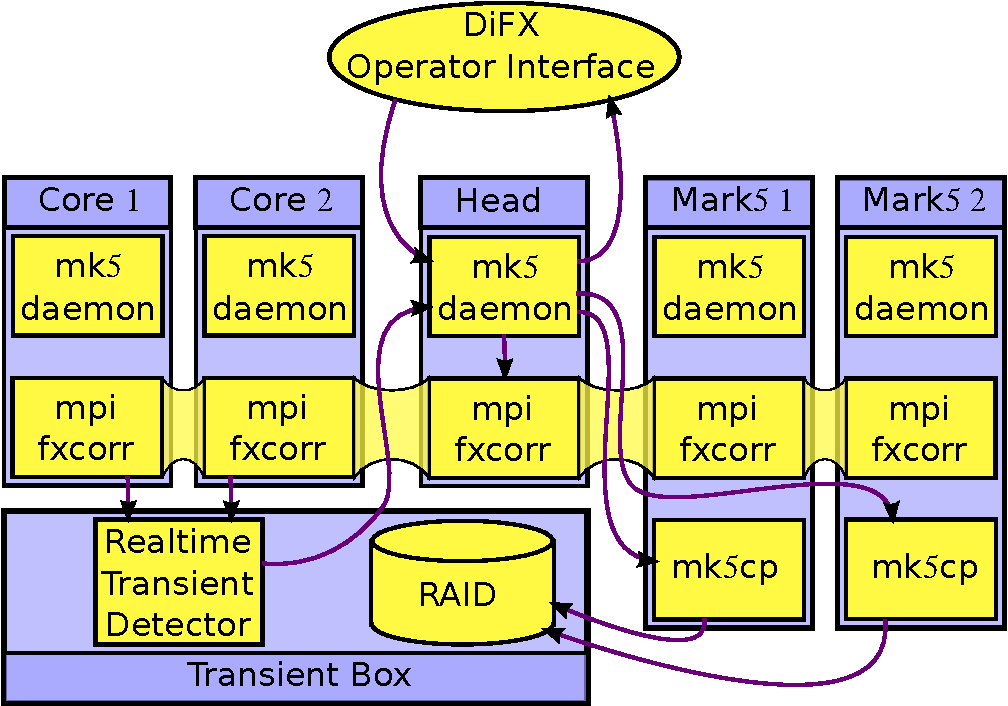
\includegraphics{transient}}
\caption[blockdiagram]{
{{\em The sequence of events leading to transient data capture.}
First the DiFX Operator Interface sends a {\tt DifxStart} message to the head node, causing the {\tt mpifxcorr} process to be started.
The core nodes of {\tt mpifxcorr} will transmit autocorrelation data to a real-time transient detection algorithm.
As interesting events are identified, {\tt DifxTransientMessage} documents are sent to the head node; the {\tt mk5daemon} process keeps a prioritized list of events.
After correlation completes but before {\tt mk5daemon} on the head node starts a series of {\tt mk5cp} processes to run to copy the baseband data from the Mark5 modules before the next job starts.
}
\label{fig:transient}
}
\end{center}
\end{figure}





% DifxStart -------------------------------------------------------------------

\subsection{DifxStart}

This document type causes the head node to spawn a correlator job.
The doument contents describe which resources to use and which {\tt .input} file to use.

The \bfit{body} of the message contains:

\begin{quotation}
\begin{Verbatim}[commandchars=\|\[\]]
    <difxStart>
      <input>|bfit[input file]</input>
      <force>|bfit[forceOverwrite]</force>
      <manager node="|bfit[node]" />
      <datastream nodes="|bfit[nodes]" />
      <process nodes="|bfit[nodes]" threads="|bfit[count]" />
      <env>|bfit[envvar]=|bfit[value]</env>
      <difxProgram>|bfit[program]</difxProgram>
      <difxVersion>|bfit[version]</difxVersion>
      <mpiWrapper>|bfit[mpiWrapper]</mpiWrapper>
      <mpiOptions>|bfit[options]</mpiOptions>
    </difxStart>
\end{Verbatim}
\end{quotation}

In the above XML file, exactly one manager node must be supplied.
There must be at least one datastream node (one per antenna being correlated).
There must be at least one process node.
Zero or more (up to a maximum of 8) environment variables may be set.
The italicized fields are as follows:

\begin{description}
\item{\bfit{input file}} complete path to the {\tt .input} file for this correlation.
\item{\bfit{forceOverwrite}} cause any previous correlator output of this job to be deleted before starting the correlation.  A value of {\tt 1} or {\tt True} will enable overwrite.
\item{\bfit{value}} the value of the environment variable.
\item{\bfit{node}} the name of the node being assigned, e.g. {\tt mark5fx02} or {\tt swc000}.
\item{\bfit{nodes}} a list of node names.  The list members should be space or comma separated.
\item{\bfit{count}} the maximum number of threads to schedule.  If not specified, 1 will be assumed.
This applies only to process nodes.
\item{\bfit{envvar}} an environment variable to set before running mpifxcorr.
\item{\bfit{program}} the name of the software correlator executable.
This is optional and defaults to {\tt mpifxcorr} if not set.
\item{\bfit{version}} the version (e.g., {\em DIFX-1.5.4}) of DiFX to run.
\item{\bfit{mpiWrapper}} the name of the program used to start the MPI processes.
This field is optional and defaults to {\tt mpirun} if none is provided.
\item{\bfit{options}} extra options to pass to {\tt mpirun}.
This is optional; sensible defaults are assumed if not explicitly set.
\end{description}

Note that multiple {\tt <process />} tags can be specified, each with its own thread count.
Each tag's thread count only affects those nodes specified in that tag.
If {\bfit{version}} is provided, then a wrapper script called {\tt runmpifxcorr.}{\em version} is expected to be in the default path which sets the environment for the version of DiF to actuallyt run.





% DifxStatusMessage -----------------------------------------------------------

\subsection{DifxStatusMessage}

This section describes messages with \bfit{messageType} = {\tt DifxStatusMessage}.
This message type is only produced by {\tt mpifxcorr} or the programs immediately responsible for starting and stopping it.

The \bfit{body} of the message contains:

\begin{quotation}
\begin{Verbatim}[commandchars=\|\[\]]
    <difxStatus>
      <state>|bfit[state]</state>
      <message>|bfit[message]</message>
      <visibilityMJD>|bfit[visibilityMJD]</visibilityMJD>
      <weight ant=|bfit[antId] wt=|bfit[weight]>
    </difxStatus>
\end{Verbatim}
\end{quotation}

\noindent The italicized fields are as follows:

\begin{description}
\item{\bfit{state}} the state of {\tt mpifxcorr}, which must be one of the following:

\begin{tabular}{ll}
state & meaning \\
\hline
{\tt Spawning} & the {\tt mpifxcorr} processes are being started (not sent by {\tt mpifxcorr}).\\
{\tt Starting} & all the processes are ready to begin. \\
{\tt Running} & the correlator is running. \\
{\tt Ending} & the correlator has reached the end of the job. \\
{\tt Done} & the correlation has completed. \\
{\tt Aborting} & correlation is stopping early due to an error. \\
{\tt Terminating} & correlation is stopping early due to signal. \\
{\tt Terminated} & correlation has stopped early. \\
{\tt MpiDone} & all of the MPI processes have ended (not sent by {\tt mpifxcorr}). \\
{\tt Crashed} & {\tt mpifxcorr} crashed; usually sent by {\tt mk5daemon}.
\end{tabular}

\item{\bfit{message}} a string containing information for the operator.
\item{\bfit{visibilityMJD}} the time-stamp (MJD + fraction) of last completed visibility record.
\item{\bfit{antId}} the antenna id for the associated weight, ranging from 0 to $N_{\mathrm{ant}}-1$.
\item{\bfit{weight}} the data weight for the associated antenna, ranging from 0 to 1.
Note that in each XML document of this type there will in general be one \bfit{weight} value for each antenna being correlated.
\end{description}







% DifxStop --------------------------------------------------------------------

\subsection{DifxStop}

Messages with \bfit{messageType} = {\tt DifxStop} are typically sent by the DiFX Operator Interface to the {\tt mk5daemon} running on the correlator head node to cause a particular instance of DiFX to be killed.

The \bfit{body} of the message contains:

\begin{quotation}
\begin{Verbatim}[commandchars=\|\[\]]
    <difxStop>
    </difxStop>
\end{Verbatim}
\end{quotation}



% DifxVex2DifxRun ----------------------------------------- INCOMPLETE --------


% Mark5DriveStatsMessage ------------------------------------------------------

\subsection{Mark5DriveStatsMessage}

Mark5 module conditioning is done periodically to ensure top performance of Mark5 modules.
Each disk in the module gets written across its whole surface to identify bad areas and to {\em calibrate} the electronics.
One message applies to one disk of the module

The \bfit{body} of the message contains:

\begin{quotation}
\begin{Verbatim}[commandchars=\|\[\]]
    <difxDriveStats>
      <serialNumber>|bfit[serial]</serialNumber>
      <modelNumber>|bfit[model]</modelNumber>
      <size>|bfit[size]</size>
      <moduleVSN>|bfit[vsn]</moduleVSN>
      <moduleSlot>|bfit[slot]</moduleSlot>
      <startMJD>|bfit[startMJD]</startMJD>
      <stopMJD>|bfit[stopMJD]</stopMJD>
      <bin|bfit[N]>|bfit[statsN]</bin|bfit[N]>
      <type>|bfit[statsType]</type>
      <startByte>|bfit[startByte]</startByte>
    </difxDriveStats>
\end{Verbatim}
\end{quotation}

\noindent The italicized fields are as follows:

\begin{description}
\item{\bfit{serial}} the serial number of the disk.
\item{\bfit{model}} the model number of the disk.
\item{\bfit{size}} the size of the disk, in GB.
\item{\bfit{vsn}} the module Volume Serial Number (VSN).
\item{\bfit{slot}} the location of the disk within the module, from 0 to 7.
\item{\bfit{startMJD}} the time when conditioning began.
\item{\bfit{stopMJD}} the time when condtioning ended.
\item{\bfit{statsN}} the histogram count for bin \bfit{N} for \bfit{N} in the range 0 to 7.
\item{\bfit{statsType}} type of operation which is one of {\tt condition}, {\tt condition\_read}, {\tt condition\_write}, {\tt read}, {\tt write}, {\tt unknown}, {\tt test}.
\item{\bfit{startByte}} if not present, assumed to be zero; only relevant for some types of operations.
\end{description}







% Mark5StatusMessage ----------------------------------------------------------

\subsection{Mark5StatusMessage}

This section describes messages with \bfit{messageType} = {\tt Mark5StatusMessage}.
This message type cones from either {\tt mpifxcorr} or {\tt mk5daemon} (or perhaps another program that makes heavy use of Mark5 units and wishes to volunteer status information).

The \bfit{body} of the message contains:

\begin{quotation}
\begin{Verbatim}[commandchars=\|\[\]]
    <mark5Status>
      <bankAVSN>|bfit[vsnA]</bankAVSN>
      <bankBVSN>|bfit[vsnB]</bankBVSN>
      <statusWord>|bfit[statusWord]</statusWord>
      <activeBank>|bfit[activeBank]</activeBank>
      <state>|bfit[state]</state>
      <scanNumber>|bfit[scanNumber]</scanNumber>
      <scanName>|bfit[scanName]</scanName>
      <position>|bfit[position]</position>
      <playRate>|bfit[playRate]</playRate>
      <dataMJD>|bfit[dataMJD]</dataMJD>
    </mark5Status>
\end{Verbatim}
\end{quotation}

\noindent The italicized fields are as follows:

\begin{description}
\item{\bfit{vsnA}} the VSN of the module in bank A.
\item{\bfit{vsnB}} the VSN of the module in bank B.
\item{\bfit{statusWord}} a hexadecimal number with the following bits:
{\em TBD}
\item{\bfit{activeBank}} the active bank, either {\tt A} or {\tt B} for banks A and B respectively, {\tt N} if the unit is in non-bank mode, or blank if no modules are active.
\item{\bfit{state}} the state of the Mark5 unit:

\begin{tabular}{ll}
state & meaning \\
\hline
{\tt Opening} & the Streamstor card is being opened. \\
{\tt Open} & the Streamstor was successfully opened and is ready for use. \\
{\tt Close} & the Streamstor has been closed. \\
{\tt GetDirectory} & the unit is recovering the directory or finding data. \\
{\tt GotDirectory} & the unit successfully found needed data on the module. \\
{\tt Play} & the unit is playing back data. \\
{\tt PlayStart} & the unit is about to start playback. \\
{\tt PlayInvalid} & the unit is playing data, but the data is invalid. \\
{\tt Idle} & the unit is not doing anything; no process has control of it. \\
{\tt Error} & the unit is unusable due to an error. \\
{\tt Busy} & the unit is busy and cannot respect commands. \\
{\tt Initializing} & the Streamstor card is initializing. \\
{\tt Resetting} & the unit is resetting the Streamstor card. \\
{\tt Rebooting} & the unit is about to reboot. \\
{\tt Poweroff} & the unit is about to turn off. \\
{\tt NoData} & the unit is not playing data since there is none that is appropriate. \\
{\tt NoMoreData} & the unit has played all the data for the job and is stopped. \\
{\tt Copy} & data is being copied off the module to a local disk. \\
\end{tabular}

\item{\bfit{scanNumber}} the directory index number for the current scan.
This number starts at 1.
\item{\bfit{scanName}} the name associated with the current scan.
\item{\bfit{position}} the byte position being accessed. 
Note that this number can be very large ($> 2^{46}$).
\item{\bfit{playRate}} the time-averaged playback rate in Mbps.
\item{\bfit{dataMJD}} the date stamp (MJD + fraction) of the most recently read data.
\end{description}







% Mark5VersionMessage ---------------------------------------------------------

\subsection{Mark5VersionMessage} % new

This section describes messages with \bfit{messageType} = {\tt Mark5VersionMessage}.
This message comes from {\tt mk5daemon}.
It is typically broadcast once upon the start of {\tt mk5daemon} and when requested.

The \bfit{body} of the message contains:

\begin{quotation}
\begin{Verbatim}[commandchars=\|\[\]]
    <mark5Version>
      <ApiVer>|bfit[ApiVer]</ApiVer>
      <ApiDate>|bfit[ApiDate]</ApiDate>
      <FirmVer>|bfit[FirmVer]</FirmVer>
      <FirmDate>|bfit[FirmDate]</FirmDate>
      <MonVer>|bfit[MonVer]</MonVer>
      <XbarVer>|bfit[XbarVer]</XbarVer>
      <AtaVer>|bfit[AtaVer]</AtaVer>
      <UAtaVer>|bfit[UAtaVer]</UAtaVer>
      <DriverVer>|bfit[DriverVer]</DriverVer>
      <BoardType>|bfit[BoardType]</BoardType>
      <SerialNum>|bfit[SerialNum]</SerialNum>
      <DaughterBoard>
        <PCBType>|bfit[PCBType]</PCBType>
        <PCBSubType>|bfit[PCBSubType]</PCBSubType>
        <PCBVer>|bfit[PCBVersion]</PCBVer>
        <FPGAConfig>|bfit[FPGAConfig]</FPGAConfig>
        <FPGAConfigVer>|bfit[FPGAConfigVersion]</FPGAConfigVer>
      </DaughterBoard>
    </mark5Version>
\end{Verbatim}
\end{quotation}


\noindent Note that the {\tt DaughterBoard} tag and its subtags are optional and are not broadcast if a daughter board is not detected on the Mark5C unit.
The italicized fields are as follows:

\begin{description}
\item{\bfit{ApiVer}} The software API version of the Streamstor API.
\item{\bfit{ApiDate}} Date associated with the above.
\item{\bfit{FirmVer}} The version of the firmware that is loaded.
\item{\bfit{FirmDate}} Date associated with the above.
\item{\bfit{MonVer}} The version of the Monitor FPGA code.
\item{\bfit{XbarVer}} The version of the cross bar FPGA code
\item{\bfit{AtaVer}} The version of the ATA disk controller FPGA code.
\item{\bfit{UAtaVer}} The version of the UATA disk controller FPGA code.
\item{\bfit{DriverVer}} The version number of the driver code.
\item{\bfit{BoardType}} The type of Streamstor board.
\item{\bfit{SerialNum}} The serial number of the Streamstor board.
\item{\bfit{PCBType}} The type of Streamstor daughter board.
\item{\bfit{PCBSubType}} Subtype of the above, if any.
\item{\bfit{PCBVersion}} The version of the daughter board.
\item{\bfit{FPGAConfig}} Name of the FPGA configuration.
\item{\bfit{FPGAConfigVersion}} Version number of FPGA configuration.
\end{description}


\end{description}



\section{Database tables} \label{sec:database}

\vspace{-20pt}\hspace{145pt}
\difxonefive

\vspace{7pt}

A database backend (currently Oracle) is used to store certain bits of information that are important for the operation of the VLBA-DiFX correlator.
The same physical database is used to store monitor data from VLBA observations and log data from foreign stations that are processed through {\tt fs2db}.
This version of this document describes only new features, including database tables not used in the hardware correlator era and the
software that populates and uses this information.
The new software in question accesses the database through one of two mechanisms.  
Python programs use the {\tt cx\_Oracle} library and Java programs (e.g., the DiFX Operator Interface) use {\tt JAXB}.

\subsection{The DIFXQUEUE table}

The DIFXQUEUE table is used to specify the state of the correlator queue.
Each job can have a unique entry in this table.
The structure of this table is based on the FXQUEUE table used by {\tt OMS}, but this table is incompatible with {\tt OMS} and should be treated as a completely parallel development.
The program {\tt difxqueue} will populate this table for each job being staged for correlation.
Initially the STATUS field will be ``QUEUED'', but will change to one of the other options in the course of correlation.
The DiFX Operator Interface (DOI) uses this database table directly.

\begin{center}
\begin{tabular}{lll}
\hline
\hline
   \multicolumn{1}{l}{Column}
 & \multicolumn{1}{l}{Type}
 & \multicolumn{1}{l}{Comments}
\\
\hline
PROPOSAL	& VARCHAR2(10)	& The proposal code \\
SEGMENT		& VARCHAR2(2)	& Segment (epoch) of proposal, or blank \\
JOB\_PASS	& VARCHAR2(32)	& Name of correlator pass (e.g. ``geodesy'') \\
JOB\_NUMBER	& INTEGER	& Number of job in the pass \\
PRIORITY	& INTEGER	& Number indicating the priority of the job in the queue; \\
		&		& 1 is high, 2 is default, and 3 is low \\
JOB\_START	& DATE		& Observe time of job start \\
JOB\_STOP	& DATE		& Observe time of job stop \\
SPEEDUP         & FLOAT         & Estimated speed-up factor for job \\
INPUT\_FILE	& VARCHAR2(512)	& Full path of the VLBA-DiFX input file \footnote{INPUT\_FILE is the primary key for this table.} \\
STATUS		& VARCHAR2(32)	& Status of the job, perhaps ``QUEUED'', ``KILLED'', \\
		&		& ``RUNNING'', ``FAILED'', ``UNKNOWN'' or ``COMPLETE'' \\
NUM\_ANT	& INTEGER	& Number of antennas in the job \\
CORR\_TYPE      & VARCHAR2(32)  & Type of correlation (e.g., ``PRODUCTION'' or ``CLOCK'') \\
CORR\_VERSION   & VARCHAR2(32)  & The DiFX version string \\
NUM\_FOREIGN    & INTEGER       & Number of non-VLBA antennas in job \\
OUTPUT\_SIZE\_EST & INTEGER       & Estimated correlator output size (MB) \\
\hline
\end{tabular}
\end{center}

\subsection{The DIFXLOG table}

The DIFXLOG table contains a list of all correlation attempts and is basesd on the FXLOG table used by the hardware correlator and {\tt OMS}.
In the case of successful correlation, the CORR\_STATUS field will be set to ``COMPLETE'' and the SPEEDUP and OUTPUT\_SIZE fields will be set.

\begin{center}
\begin{tabular}{lll}
\hline
\hline
   \multicolumn{1}{l}{Column}
 & \multicolumn{1}{l}{Type}
 & \multicolumn{1}{l}{Comments}
\\
\hline
PROPOSAL	& VARCHAR2(10)	& The proposal code \\
SEGMENT		& VARCHAR2(2)	& Segment (epoch) of proposal, or blank \\
JOB\_PASS	& VARCHAR2(32)	& Name of correlator pass (e.g. ``geodesy'') \\
JOB\_NUMBER	& INTEGER	& Number of job in the pass \\
CORR\_START	& DATE		& Start time/date of correlation \\
CORR\_STOP	& DATE		& Stop time/date of correlation \\
SPEEDUP         & FLOAT         & Measured speed-up factor \\
INPUT\_FILE     & VARCHAR2(512) & File name of .input file \\
OUTPUT\_FILE	& VARCHAR2(512)	& File name of correlator output \\
OUTPUT\_SIZE	& INTEGER	& Size (in $10^6$\,bytes) of correlator output \\
CORR\_STATUS	& VARCHAR2(32)	& Status of correlation, typically ``COMPLETED'' \\
CORR\_TYPE      & VARCHAR2(32)  & Type of correlation (e.g., ``PRODUCTION'' or ``CLOCK'') \\
CORR\_VERSION   & VARCHAR2(32)  & The DiFX version string \\
\hline
\end{tabular}
\end{center}

\subsection{The CONDITION table}

The CONDITION table contains performance information for the hard disks comprising Mark5 modules.
A separate table entry is made for each disk in a module so typically there will be 8 entries generated for each module conditioned.
There are two paths to get data into this table.
The {\tt condition} program can be used to manually load condition reports from the SSErase program.
Secondly, the {\tt condition\_watch} program automatically populates the database immediately after module conditioning upon receipt of a {\tt Mark5ConditionMessage} that is now generated by a specially modified version of Haystack Observatory's {\tt SSErase} program.

\begin{center}
\begin{tabular}{lll}
\hline
\hline
   \multicolumn{1}{l}{Column}
 & \multicolumn{1}{l}{Type}
 & \multicolumn{1}{l}{Comments}
\\
\hline
SERIALNUM       & VARCHAR2(32)	& The hard disk serial number \\
MODEL           & VARCHAR2(32)  & Model number of hard disk \\
CAPACITY        & INTEGER       & Size of disk in $10^9$ bytes \\
MODULEVSN       & VARCHAR2(10)  & The name of the module containing the disk \\
SLOT            & INTEGER       & The slot number within the module (0 to 7) \\
STARTTIME       & DATE          & Date/time of conditioning start \\
STOPTIME        & DATE          & Date/time of conditioning completion \\
BIN0            & INTEGER       & Bin 0 of performance histogram ($<$ 1.125 ms) \\
BIN1            & INTEGER       & Bin 1 of performance histogram ($<$ 2.25 ms) \\
BIN2            & INTEGER       & Bin 2 of performance histogram ($<$ 4.5 ms) \\
BIN3            & INTEGER       & Bin 3 of performance histogram ($<$ 9 ms) \\
BIN4            & INTEGER       & Bin 4 of performance histogram ($<$ 18 ms) \\
BIN5            & INTEGER       & Bin 5 of performance histogram ($<$ 36 ms) \\
BIN6            & INTEGER       & Bin 6 of performance histogram ($<$ 72 ms) \\
BIN7            & INTEGER       & Bin 7 of performance histogram ($\ge$ 72 ms) \\
\hline
\end{tabular}
\end{center}


\section{DiFX alert messages} \label{sec:messages}

This section attempts to list all of the messages you might see coming from the software correlator with some explanation about their meaning.
For some messages, certain actions to be taken are suggested.
Each subsection below contains descriptions of the messages for a particular severity level, ordered from most severe to least severe.
There are almost 500 distinct messages that could be produced by {\tt mpifxcorr} as of DiFX version 1.5.2, thus no effort has been made to be compete in the descriptions here.
Effort has been made to document the most important ones in detail.
Messages are sorted first by their severity level and are then roughly alphabetical within each subsection.




\subsection{Fatal}

All fatal errors will cause immediate termination of the correlation project.
Most such errors would occur at the very start of a job as the input files are being processed.

\begin{itemize}

\item {\bf Bin phase breakpoints are not in linear ascending order!!!}:
The pulsar bins are not listed in phase order in the {\tt .binConfig} file.
Each {\tt BIN PHASE END} entry must be greater than the previous and they must all be in the range 0 to 1.

\item {\bf Cannot create output directory {\it outDir}: {\it flag} - aborting!!!}:
The output directory could not be created.
The most common cause is an existing output file from a previous attempt to correlate the job in question.
Other possible causes include: permission issues, inaccessibility of output directory to the DiFX head node, and output filesystem being full.

\item {\bf Cannot locate {\it stationName} in delay file {\it delayFile} - aborting!!!}:
The specified delay file does not contain needed information for a station called {\it stationName}.
This should never happen for data going through the correlator in a standard way.

\item {\bf Cannot open Streamstor device.  Either this Mark5 unit has crashed, you do not have read/write permission to /dev/windrvr6, or some other process has full control of the Streamstor device.}:
This message will only come from a Mark5 unit that is requested to play back data.
The most likely cause of such a problem is the Streamstor card getting stuck in a compromised state, although fresh correlator installations that may not have left {\tt /dev/windrvr6} with global read/write permission is a second likely cause of this problem.
The fix likely requires a reboot of the Mark5 unit.
On occasion a full power cycle of the Mark5 unit (not just a soft reboot) is required.

\item {\bf Cannot open file {\it inputFile} - aborting!!!}:
The {\tt .input} file named {\it inputFile} is not readable by the software correlator.
This could be due to one of a number of issues, including: read permission problems, the request file not existing, or the file existing but not visible from one or more of the software correlator nodes.

\item {\bf Cannot open delay file {\it delayFile} - aborting!!!}:
The {\tt .delay} file named {\it delayFile} is not readable by the software correlator.
This could be due to one of a number of issues, including: read permission problems, the request file not existing, or the file existing but not visible from one or more of the software correlator nodes.

\item {\bf Cannot open output file {\it outputFile} - aborting!!!}:
The output file could not be created.
The most common cause is an existing output file from a previous attempt to correlate the job in question.
Other possible causes include: permission issues, inaccessibility of output directory to the DiFX head node, and output filesystem being full.

\item {\bf Cannot open pulsar config file {\it binConfigFile} - aborting!!!}:
The specified pulsar bin file, {\it binConfigFile} cannot be opened.
This could be due to one of a number of issues, including: read permission problems, the request file not existing, or the file existing but not visible from one or more of the software correlator nodes.

\item {\bf Cannot open uvw file {\it uvwFile} - aborting!!!}:
The specified {\tt .uvw} file, {\it uvwFile} cannot be opened.
This could be due to one of a number of issues, including: read permission problems, the request file not existing, or the file existing but not visible from one or more of the software correlator nodes.

\item {\bf Cannot quad interpolate delays with post-f fringe rotation - aborting!!!}:
Two mutually exclusive options ({\tt QUAD DELAY INTERP} and {\tt POST-F FRINGE ROT}) were both enabled in the {\tt .input} file.

\item {\bf Caught an MPI exception!!! {\it errorString}}:
A process communication error has occured causing the correlator to terminate.
The outcome of such an event cannot be good; contact a DiFX developer.

\item {\bf Config encountered inconsistent setup in config file - aborting!!!}:
One or more of the configurations (group of settings defined in the {\tt .input} file) is either illegal or incompletely defined.
Usually this message will come with another more detailed error message.
In any case, either there is a correlator version mismatch or there is something wrong with the {\tt .input} file.

\item {\bf Core received a request to process data from time {\it time} which does not have a config - aborting!!!}:
This is likely due to failed consistency check in the software correlator that resulted from a logic error in the code.
This should be reported to a DiFX developer.

\item {\bf Could not find station {\it stationName} in the uvw file when making rpfits header!!!  This station is used in the correlation so I will abort!!!}:
This error only occurs with RPFITS output format which is not supported by this documentation -- please seek other sources of assistance if needed.

\item {\bf Could not locate any of the specified sources in the specified time range - aborting!!!}:
The correlator gave up since none of the sources to be correlated appeared in the {\tt .uvw} file.
This should never happen for data going through the correlator in a standard way.

\item {\bf Could not locate a polyco to cover the timerange ...}:
A pulsar polynomial for a certain time period could not be found.
The person supplying the puslar polynomial should be contacted.

\item {\bf DataStream assumes long long is 8 bytes, it is {\tt x} bytes - aborting!!!}:
This should not occur on any modern operating system.
If this message is seen, please contact a DiFX developer and be sure to indicate exactly which operating system and computer type you are using.

\item {\bf DataStream assumes int is 4 bytes, it is {\it x} bytes - aborting!!!}:
This should not occur on any modern operating system.
If this message is seen, please contact a DiFX developer and be sure to indicate exactly which operating system and computer type you are using.

\item {\bf DataStream {\it mpiid}: expected {\it x} bytes, got {\it y} bytes - aborting!!!}:
In an eVLBI read, the wrong number of bytes was received, indicating a mismatch in send/receive setups.
Check the setup at both ends and try again.

\item {\bf Datastream {\it mpiid}: implied UDP packet size is negative - aborting!!!}:
When considering the size of a UDP header, an unphysical packet size results.
This should only occur when attempting UDP based eVLBI.

\item {\bf Datastream {\it mpiid}: read too few UDP packets: bytestoread={\it x} udp\_offset={\it y} bytes={\it z} - aborting!!!}:
Fewer than expected UDP packets were received in an eVLBI transfer (FIXME -- more details please!)

\item {\bf Datastream {\it mpiid}: read too many UDP packets: bytestoread={\it x} udp\_offset={\it y} bytes={\it z} - aborting!!!}:
More than expected UDP packets were received in an eVLBI transfer (FIXME -- more details please!)

\item {\bf Datastream {\it mpiid}: could not allocate databuffer (length {\it size}) - aborting!!!}:
A memory allocation failed.
This would probably be due to either a developer error or attempt to run a job on an underpowered computer. 
In any case, the developer should be contacted.

\item {\bf Developer error: Cannot handle delays more negative than {\it maxDelay}. Need to unimplement the datastream check for negative delays to indicate bad data - aborting!!!}:
The maximum negative delay (which is quite large) has been exceeded.
This is almost certainly a logic error in the software and should be reported to a DiFX developer.

\item {\bf Developer error: in Mk5Mode::Mk5Mode, mark5stream is null}:
An internal error related to initializing a Mark5 decoder has occurred.
Contact a DiFX developer.

\item {\bf Developer error: in Mk5Mode::Mk5Mode, framesamples is inconsistent ({\it x}/{\it y})}:
An internal inconsistency has been found in the Mark5 data frame size that would lead to downstream errors.
This could only be caused by a software logic error.
Contact a DiFX developer.

\item {\bf Developer error: UVW has not been created!!!}:
This message would come from an internal consistency check that failed.
If this occurs, the DiFX developers should be notified as this indicates a logic error inside the software correlator.

\item {\bf genMk5FormatName : {\it formatType} format : framebytes = {\it frameBytes} is not allowed}:
An illegal frame size was specified in the {\tt .input} file.
This should never happen for data going through the correlator in a standard way.
If you see this message it is probably due to a programming error and the DiFX developers should be notified.

\item {\bf genMk5FormatName : unsupported format encountered}:
A data format not handled by the software correlator has been requested in the {\tt .input} file.

\item {\bf Input file out of order!}:
There is an error in the input file.
This might be caused by using an input file formatted for one version of {\tt mpifxcorr} on a different version or by an incorrectly written file.

\item {\bf Manager aborting correlation!}:
The configuration of a visibility buffer was not OK.
There are many possible causes for this, but is most likely due to a logic error in the software.
Contact a DiFX developer if this is encountered.

\item {\bf Mk5DataStream::readnetwork bytestoread too large ({\it x}/{\it y}) - aborting!!!}:
An eVLBI read size is too large. (FIXME -- more details here please!)

\item {\bf mpifxcorr must be invoked with at least {\it x} processors (was invoked with {\it y} processors) - aborting!!!}:
For a correlation of $N$ datastreams (usually equal to the number of antennas), at least $N+2$, but preferably even more, processes must be started.

\item {\bf NativeMk5DataStream::NativeMk5DataStream stub called, meaning mpifxcorr was not compiled for nativemk5 support, but it was requested (with MODULE in .input file) - aborting!!!}:
Correlation directly off a Mark5 module requires compiling against the Streamstor libraries which was apparently not done but requested by the {\tt .input} file.
Contact the person responsible for your correlator setup and ask them to properly link the Streamstor libraries to the {\tt mpifxcorr} executable.

\item {\bf No config section in input file}:
The input file is missing its config section and hence correlation cannot proceed.
This should never happen for data going through the correlator in a standard way.

\item {\bf Not enough baselines are supplied in the baseline table ({\it x}) compared to the number of baselines ({\it y})!!!}:
The {\tt .input} file requests more baselines in the common table than there are enumerated in the baseline table.
This should never happen for data going through the correlator in a standard way.

\item {\bf Not enough datastreams are supplied in the datastream table ({\tt x}) compared to the number of datastreams ({\tt y})!!!}
The {\tt .input} file requests more datastreams (nominally equal to the number of antennas) in the common table than there are enumerated in the baseline table.
This should never happen for data going through the correlator in a standard way.

\item {\bf Please invoke with mpifxcorr ...}:
The correlator was not started according to is usage.
See \S\ref{sec:mpifxcorr} for more details.

\item {\bf Polyco {\it polycoId} / {\it subcount} is malformed}
The pulsar polynomial file is not compliant (possibly due to manual editing).

\item {\bf RPFITS not compiled in - aborting}:
RPFITS output format is requested, but support for RPFITS is not compiled into {\tt mpifxcorr}.
Either requested output format, or recompile {\tt mpifxcorr} with RPFITS.
Note: This document does not contain instructions for RPFITS installations -- you are on your own!

\item {\bf Samplesperblock is less than 1, current implementation cannot handle this situation - aborting!!!}:
An illegal data sub-mode has been requested.
Contact a developer.

\item {\bf Unknown data format {\it formatName}}:
A data format (e.g., VLBA, Mark4, LBA) has been requested that cannot be processed.

\item {\bf Unknown data source {\it sourceName}}:
A data source (e.g., FILE, MODULE, EVLBI) has been requested that cannot be used.

\end{itemize}





\subsection{Severe}

Severe errors typically reflect an unexpected software error.
All severe errors are related to a process control (threading) failure or a failure in a numerical routine.
Errors of the severe type are likely to cause widespread erroneous results or complete failure of correlation.
Except during periods of software development errors of these two types are unexpected.
If encountered, they should be reported to a DiFX developer and the correlation should be reattempted once.
Since there are many errors in the ``severe'' class, all unlikely and with the same procedure for working around, individual errors of this type are not listed below.





\subsection{Error}

Messages in the ``Error'' class are typically fairly significant, often cascading to fatal messages and termination of the correlation.
Many errors of the Mark5 variety result data loss ranging from fractions of a second to the full job in length.
For errors of this type, operator judgement is needed: whether to restart correlation or keep going will depend on many circumstances.
Note that many of the eVLBI and real-time monitor errors are not documented here yet.

\begin{itemize}

\item {\bf All data from this module was discarded: ...}:
Due either to malformed data or a directory file with incorrect values, no data was deemed suitable for correlation for a particular Mark5 module.
It is probably worth trying to extract the module directory structure again and trying the job again and/or moving the module to a different unit for playback.
It is likely that other jobs using this module will face a similar problem.

\item {\bf {\it n} consecutive sync errors.  Something is probably wrong!}:
A large number of sync errors were seen.
This probably means that the Mark5 data being read is somehow corrupted.

\item {\bf All bandwidths for a given datastream must be equal}:
Currently, {\tt mpifxcorr} does not allow different bandwidths on different frequency bands.
This will lead to temination of the correlator.
The creator of the {\tt .input} file should be contacted.

\item {\bf All configs must have the same telescopes!  Config {\it m} datastream {\it n} refers to different telescopes}:
The same set of telescopes (antennas) must be used throughout a job.
Two configurations have been found that use different antenna subsets.
This will lead to temination of the correlator.
The creator of the {\tt .input} file should be contacted.

\item {\bf All LBASTD Modes must have 2 bit sampling - overriding input specification!!!}:
The Australian LBASTD data format modes can only handle 2-bit (4 level) quantization at the moment.
The {\tt .input} file value for {\tt QUANTISATION BITS} is being ignored here.
Probably the maker of the {\tt .input} file made a mistake.

\item {\bf Attempting to get a delay from offset time {\it time}, will take {\tt first}|{\tt last} source}:
Correlation is requested for a time either before or after the list of scans.
Data affected by this is likely to have the wrong delay applied and is unlikely to be useful.
The creator of the input files should be contacted.

\item {\bf Attempting to refer to freq outside local table!!!}:
The frequency index of a datastream table exceeds the length of the frequency table in the {\tt .input} file.
This will most certainly cause this frequency band to be incorrectly correlated.

\item {\bf Baseline table entry {\it m}, frequency {\it n}, polarisation product {\it p} for datastream {\it q} refers to a band outside datastream {\it q}'s range ({\it r})}:
The band index for a baseline table exceeds its legal range.
This will lead to temination of the correlator.
The creator of the {\tt .input} file should be contacted.

\item {\bf Baseline table entry {\it m} has a datastream index outside the datastream table range! Its two indices are {\it n}, {\it p}}:
The baseline table has a datastream index that exceeds the number of
datastreams.
This will lead to temination of the correlator.
The creator of the {\tt .input} file should be contacted.

\item {\bf Cannot clear Mark5 write protect}:
The software correlator attempts to set the Disk Module State to {\tt PLAYED}.
This requires temporarily disabling write protection.
If this fails, then either the Mark5 unit is in a bad state or the module has a problem.

\item {\bf Cannot open data file {\it dataFile}}:
The datastream process cannot open the specified file containing baseband data to be correlated.
Correlation will proceed, but no data for an antenna for the duration of this file will be correlated.
Usually this error should be a cause for concern.

\item {\bf Cannot open polyco file {\it polycoFile}}:
Either file permissions, file location, or non-existence is preventing the file called {\it polycoFile} from being opened.
This will likely end badly.

\item {\bf Cannot put Mark5 unit in bank mode}:
The command to put the Mark5 unit in single bank mode failed and further commands to the Mark5 unit will probably fail as well.
Usually this only happens if the Mark5 unit is in a bad state.
The Mark5 unit probably needs a reboot.

\item {\bf Cannot read data from Mark5 module...}:
Read from a Mark5 module failed.
No further attempt to read data from the module will be made.
It is strongly recommended that the Mark5 unit be rebooted and the correlation be reattempted.
If the error is reproducible, the additional information contained at the end of this error message may help diagnose the problem.

\item {\bf Cannot read the Mark5 module label}:
The command to retrieve the module label, which includes the volume serial number (VSN) and the previous state, has failed.
This implies trouble with the Mark5 unit or module.
First the module should be moved to a different Mark5 unit and the correlation reattempted.
Upon further failure, the module should be checked for problems

\item {\bf Cannot set Mark5 data replacement mode / fill pattern}:
Either the command to tell the Mark5 unit to enter real-time playback mode or the command to set the fill pattern have
failed; expect more problems with this Mark5 unit.
The Mark5 unit probably needs a reboot.

\item {\bf Cannot set the Mark5 module state}:
The software correlator failed to set the Disk Module State to {\tt PLAYED}.
If this fails, then either the Mark5 unit is in a bad state or the module has a problem.

\item {\bf Cannot set Mark5 write protect}:
The software correlator attempts to set the Disk Module State to {\tt PLAYED}.
This requires temporarily disabling write protection.
If this fails, then either the Mark5 unit is in a bad state or the module has a problem.

\item {\bf Cannot unpack Mark5 format data at sampleoffset {\it n} from buffer {\it time}}:
An error of this kind likely represents a logic error in the software correlator and should be reported to a DiFX developer.

\item {\bf Config {\it m} baseline index {\it n} refers to baseline {\it p} which is outside the range of the baseline table}:
The baseline index of a config table exceeds the number of baselines in the baseline table.
This will lead to temination of the correlator.
The creator of the {\tt .input} file should be contacted.

\item {\bf Config {\it m} baseline index {\it n} refers to baseline {\it p} which is out of order with the previous baseline ...}:
Entries in the datastream table are not in the expected order.
This will lead to temination of the correlator.
The creator of the {\tt .input} file should be contacted.

\item {\bf Could not find a polarisation pair, will be put in position {\it x}\,!!!"}:
This is due either to an uncaught inconsistency in the {\tt .input} file or a logic error in the software correlator.
Contact a DiFX developer.

\item {\bf Could not find any bands for frequency {\it m} of datastream {\it n}}:
This is due either to an uncaught inconsistency in the {\tt .input} file or a logic error in the software correlator.
Contact a DiFX developer.

\item {\bf Could not open {\it threadFile} - will set all numthreads to 1!!!}:
The requested {\tt .threads} file could not be opened.
Possible causes include: permission issues, inaccessibility of directory to the DiFX head node, and the file simply not existing.
The impact of this is that correlation will proceed at a potentially much reduced speed since each CPU will use only a single processing thread.
Accuracy of the results will not be affected.

\item {\bf Could not parse LBA file header}:
An LBA format file appears corrupt.
Data for one antenna for the duration of this file will not be correlated.

\item {\bf Datastream table entry {\it m} has a frequency index (freq {\it n}) that refers outside the frequency table range ({\it p})}:
The {\tt .input} file has a frequency index error.
This will lead to temination of the correlator.
The creator of the {\tt .input} file should be contacted.

\item {\bf Datastream table entry {\it m} has an input band local frequency index (band {\it n}) that refers outside the local frequency table range ({\it p})}:
The {\tt .input} file has a frequency index error.
This will lead to temination of the correlator.
The creator of the {\tt .input} file should be contacted.

\item {\bf Datastream table entry {\it m} has a telescope index that refers outside the telescope table range ({\it n})}:
The {\tt .input} file has a telescope index error.
This will lead to temination of the correlator.
The creator of the {\tt .input} file should be contacted.

\item {\bf FFT chunk time for config {\it m}, datastream {\it n} is not a whole number of nanoseconds ({\it p})}:
In order to keep track of time properly, each FFT must start on an integer nanosecond boundary.
There are currently no modes supported where this should be a problem, so if you see this message, there is a more serious problem.
Contact a DiFX developer!

\item {\bf First datastream for baseline {\it n} has a higher number than second datastream - reversing!!!}:
The entries of the baseline table (indicating which antenna pairs to correlate) should always have the datastream indices in ascending order.
If you see this warning, the correlator is correcting your baseline ordering, but be aware that this might be hinting that something else might be awry with the {\tt .input} file.
The creator of the {\tt .input} file should be contacted.

\item {\bf Hit the end of the file! Setting the numthread for Core {\it n} to 1}:
The {\tt .threads} file ended unexpectedly early and one or more core processes will be forced to use a single processing thread, with potentially crippling performance penalty.
Accuracy of the results will not be affected.

\item {\bf Increment per read in nanoseconds is {\it x} - too large to fit in an int}:
The way timekeeping works in DiFX, data chunks larger than $2^{31}-1$ nanoseconds in length are not possible at the moment.
The maker of the {\tt .input} file needs to reduce the read size by
changing some of the parameters (such as {\tt NUM CHANNELS}, {\tt BLOCKS PER SEND}, or possibly others).

\item {\bf lastoffsetns less than 0 still! = {\it x}}:
This message probably indicates a logic error in the correlator program so should be reported to a DiFX developer.

\item {\bf Mk5DataStream::calculateControlParams : vlbaoffset={\it x} bufferindex={\it y} atsegment={\it z}}:
A Mark5 data frame was found unaligned.
A corresponding subintegration of data will be invalidated.
A large number of messages of this type probably indicates corrupted data.

\item {\bf Module {\it VSN} contains undecoded scans!}:
The module directory for module {\it VSN} has problems.
Please correct the problem with the directory (as stored in {\tt \$MARK5\_DIR\_PATH}) and try again.

\item {\bf Module {\it VSN} not found in unit!}:
The {\tt .machines} file suggested that a specified Mark5 module would be found this this Mark5 unit but it was not.
Check to make sure the module is in the unit.

\item {\bf Most of the data from this module was discarded: ...}:
Due either to malformed data or a directory file with incorrect values, a large fraction of the data for this job from a particular module was not decodable.
It is probably worth trying to extract the module directory structure again and trying the job again and/or moving the module to a different unit for playback.
It is likely that other jobs using this module will face a similar problem.

\item {\bf No valid data found.  Stopping playback!}:
According to the directory for the module in question there is no valid data available to correlate.
It is possible that a directory reconstruction will allow some or all of the data on the module to be retrieved.

\item {\bf Not all datastreams accounted for in the datastream table for config {\it m}}:
All datastreams (roughly equivalent to antennas) must be represented in each configuration within the {\tt .input} file.
This will lead to temination of the correlator.
The creator of the {\tt .input} file should be contacted.

\item {\bf Number of input bands for datastream {\it m} ({\it n}) does not match with Mark5 file {\it fileName} ({\it p}), will be ignored!!!}:
The description of Mark5 baseband data (VLBA or Mark4 format) in the {\tt .input} file is inconsistent with the actual content.
The creator of the {\tt .input} file should verify that the format is correctly specified.
All data related to this condition will be left uncorrelated.

\item {\bf Oversamplefactor ({\it m}) is less than decimation factor ({\it n})}:
The oversample factor must be an integer $r$ times the decimation factor.
Essentially oversampling is handled by two mechanisms: decimation of the input data stream in the data unpacker and through spectral selection at the time of FITS file creation.  The oversampling factor of these two approaches must multiply to be the total {\it Oversamplefactor}.
This will lead to temination of the correlator.
The creator of the {\tt .input} file should be contacted.

\item {\bf Pulsar phase as calculated fromt the polyco will not be accurate over entire range of {\it time} as the frequency is changing too rapidly.  The maximum safe calc length would be {\it x} - try reducing blocks per send or numchannels ...}:
A detail of the way the pulsar polynomial is used is likely to cause imperfect binning.
Please consult with the PI and the creator of the {\tt .input} file.

\item {\bf Stale data was received from core {\it n} regarding time {\it time} seconds - it will be ignored!!!}:
One subintegration of data is being discarded as it did not arrive in time for the data to be written to disk.
If this is a chronic problem, increasing the value of {\tt VIS BUFFER LENGTH} in the {\tt .input} might help.
A small number of errors of this type is not a problem.

\item {\bf Telescope {\it antName} could not be found in the uvw file!!!}:
Data for this antenna will not have useful UVW values in its output file.
Contact the creator of the {\tt .input} file.

\item {\bf There must be an integer number of sends per datasegment.  Presently databufferfactor is {\it m}, and numdatasegments is {\tt n}}:
The {\tt .input} file contains an inconsistency in its parameterization of the various buffer sizes.
This will lead to temination of the correlator.
The creator of the {\tt .input} file should be contacted.

\item {\bf Trying to read past the end of file!!!}:
One of the files read by {\tt mpifxforr} ended prematurely.
The maker of the {\tt .input} file should be contacted.

\item {\bf Unknown output format {\it outFormat} (case sensitive choices are RPFITS, SWIN and ASCII)}:
{\tt mpifxcorr} currently supports 3 output formats (ASCII, DIFX and RPFITS) and the requested one does not match one of these.  
This will lead to temination of the correlator.
The creator of the {\tt .input} file should be contacted.

\item {\bf Unsupported format or mode requested!!!}:
A data format has been requested that is recongnized but not supported by the correlator.
Scans using this format (probably all scans for the antenna in question) will produce no data.
The maker of the {\tt .input} file should be contacted.

\item {\bf Waited 6 seconds for a Mark5 read and gave up.}:
A Mark5 read timed out.
A small number of such errors can be tolerated, especially for a module that is known to be bad, but many such messages
should prompt a second correlation attempt after module move / unit reboot.

\item {\bf We thought we were reading something starting with '{\it something}', when we actually got '{\it somethingElse'}}:
The ordering or content of one of the files being read by {\tt mpifxcorr} does not match expectations and is thus non-conformant.
The maker of the file should be contacted.
Note that this could be caused by a version mismatch between in the input files and the correlator.

\item {\bf XLRCardReset() failed.  Remainder of data from this antenna will not be correlated and a reboot of this Mark5 unit is probably needed.}:
It is probably worth reattempting correlation after Mark5 reboot and possible module move.

\item {\bf XLROpen() failed.  Remainder of data from this antenna will not be correlated and a reboot of this Mark5 unit is probably needed.}:
After a successful Streamstor card reset, the card was not able to be accessed.
It is probably worth reattempting correlation after Mark5 reboot and possible module move.

\end{itemize}





\subsection{Warning}

Warning level messages typically relate to a situation that may result in the loss of a very small amount of data or indicate some other irregularity to the operator.
A single warning should not be of concern, but a large number of warnings should be noted.

\begin{itemize}

\item {\bf {\it n} consecutive fill patterns at time {\it time}}:
Instead of reading data from the module, the Streamstor card returned fill pattern for this many consecutive data frames.
If the module is flakey, it may be possible to recover more data after moving the module to a different Mark5 unit, but usually warnings of this type indicate inevitable data loss due to fill pattern replacement.

\item {\bf {\it n} consecutive sync errors starting at readpos {\it p} ...}:
Data was read off the module, but the sync word was not found.
This either indicates attempted playback of the wrong data format, completely corrupted data, or valid data that has slipped samples and is thus unfortunately not processable by the software correlator.
It might be worth a recorrelation attempt after moving the module, but not likely.

\item {\bf Cannot find a valid configindex to set Mk5-related info.  Flagging this subint}:
Application of the delay model caused a small amount of data to cross a scan boundary in a manner that required the flagging of an entire subintegration.
Such an event should be very rare.

\item {\bf Connection to monitor socket still pending}:
When real-time monitoring of the output visibilities is requested but no connection to a monitor program has been establish this warning may appear.
A warning of this type is not associated with any data loss.

\item {\bf Copying a polyco with no frequency information!}:
A pulsar polynomial without frequency information has been found.
This could present problems in setting the gate properly across frequency channels, but could be intentional.

\item {\bf Could not find station {\it stationName} in the uvw file when making rpfits header!!!  This station is not used in this correlation so its parameters will be initialised to 0!!!}:
The {\tt .input} file included a station not in the {\tt .uvw} file, but this station is not used so the results won't be affected.
This warning will only be issued for data being written in RPFITS format.
The resultant RPFITS file will still list the missing antenna, but it's information will be bogus.
This could confuse downstream software.

\item {\bf Could not open command monitoring socket! Aborting message receive thread.}:
Real-time monitoring was wanted, but a problem at the operating system level (perhaps permissions?) prevented the needed socket from being created.
This has no bearing on the quality of the output data.

\item {\bf Data was received which is too recent ({\it x}\,sec + {\it y}\,ns)! ...}:
A portion of one visibility record will have incomplete weight due to forced flushing of the long term accumulator buffer for that visibility record.
A single warning of this type on source change is nothing to worry about, but constant warnings of this should be reported as this may indicate a different problem.

\item {\bf DataStream {\it mpiid}: could not identify Mark5 segment time ({\it formatName})}:
An eVLBI data packet could not be decoded and hence its time cannot be determined.
This is usually not a problem since time can be dead-reckoned from previous data and the corrupt packet won't be used anyway.

\item {\bf Filterbank not yet supported!!!}:
The filterbank mode, enabled with the {\tt FILTERBANK USED} option in the {\tt .input} file, was requested, but is currently not supported.
When supported, the filterbank mode will offer options for {\em crisper} spectral channels.

\item {\bf Fractional start time of {\it x} seconds plus {\it y} ns was specified, but the start time corresponded to a configuration not specified in the input file and hence we are skipping {\it z} seconds ahead! The ns offset will be set to 0!!!}:
This warning indicates that the start time of the job is not contained within a scan to be correlated and the subsequent start time will be rounded to the next integer second.
Except in cases where exact timestamp matching is needed this is not a problem.
The warning is issued as it is not normal for the start time of a job to be outside a scan.
If you see this a lot, contact the person generating your jobs and let them know.

\item {\bf FXMANAGER caught a signal and is going to shut down the correlator}:
A terminate signal was sent to the manager process indicating that the correlator should be stopped immediately.
The resultant output file will be incomplete, but the early stop was probably on purpose so that should be expected.

\item {\bf Hit end of first line prematurely - check your polyco conforms to standard! Some values may not have been set properly, but likely everything is ok}:
The pulsar polynomial file had an unexpectedly short first line.
Some parameters may not have been properly set so the pulsar gating may not work.
Retrying correlation will not help!
If you are concerned, contact the producer of the polynomial.

\item {\bf Hit end of second line prematurely - check your polyco conforms to standard! Some values may not have been set properly.  This often happens for non-binary pulsars.  Likely everything is ok.}
It is possible that the pulsar polynomial file is incomplete, but more likely nothing is wrong.

\item {\bf Incorrectly set config index at scan boundary! Flagging this subint}:
A subintegration that crosses the end of a scan got flagged as a result of a potential format change at this time.
This should happen no more than once per scan and affects only a small fraction of one integration period in most cases.

\item {\bf Internal Error, trying to copy pass buffer size}:
This is an eVLBI related error.  (FIXME -- please add more description here)

\item {\bf Mk5DataStream::calculateControlParams : bufferindex={\it x} $>=$ bufferbytes={\it y}}:
A fraction of a dataframe is being discarded due to a frame misalignment.
This affects a very small amount of data and should be very rare.

\item {\bf Module label is not terminated!}:
A Mark5 module has an oversized extended serial number label.
This in itself is not a problem but may inidicate either corruption on the module or poor seating of either the Mark5 module or one of the cables/cards inside the Mark5 unit.

\item {\bf Module label record separator not found!}:
No ``Disk Module State'' was stored on this module.
This is probably due to recording on a very old version of Mark5A or is possibly the result of some other incompatibility.

\item {\bf MPI Id {\it mpiid}: warning - received a parameter instruction regarding {\it paramName} which cannot be honored and will be ignored!}
The software correlator can receive a number of different commands that can affect its dumping of its long-term accumulator to an external piggy-back processor.
If an unrecognized parameter is received a warning of this type will be issued.
This is completely unrelated to correlator data quality.

\item {\bf No more data for project on module {\it mpiid}}:
Although data on the module extends past the end of the current job, none of the remaining data is relevant for this job so playback is stopping early.
This is only a problem if it is due to an incorrect transcription of the module directory.
It might be prudent to look at the observe log to see if data is expected.

\item {\bf No more data on module {\it mpiid}}:
The Mark5 unit sending this message is stopping its reading before the end of the job since no more data exists.
This is only a problem if it is due to an incorrect transcription of the module directory.
It might be prudent to look at the observe log to see if data is expected.

\item {\bf Post-f fringe rotation not yet tested - use at your own risk!!!}:
Post FFT fringe rotation (enabled with the {\tt POST-F FRINGE  ROT} {\tt .input} file option) has not been extensively tested.
Results may be OK, but you are on your own!

\item {\bf Trying to read {\it s} seconds past the end of the UVW array!}:
The {\tt .uvw} file does not cover an entire scan.
If more than a couple such warnings are seen, the creator of the {\tt .input} and {\tt .calc} file should be notified.

\item {\bf Waited {\it s} sec state={\it state}}:
A Mark5 module is taking longer than expected to respond.
Additional messages will follow if this situation is serious.

\item {\bf XLRCardReset() being called!}:
If a read timeout occurs, the Streamstor card in the Mark5 unit will be reset.
This message indicates that this non-standard procedure is occuring.
The result of this reset will usually either be success (in which case a message will indicate such), failure (in which case an error message will state that no more data will be read from the module), or a Mark5 unit hang, and hence the correlation will stop.
If this is not successful, it is recommended that the correlation be retried after rebooting the affected Mark5 unit and possibly moving the module to a different Mark5 unit.

\end{itemize}

\subsection{Info}

Info messages convey normal messages to the operator.

\subsection{Verbose}

Verbose messages convey normal messages to the operator that are either not very important or come in vast quantities; they are typically filtered out of data logging to prevent unnecessary bloat.

\subsection{Debug}

Debug messages are useful only to developers and don't usually indicate error conditions.  
In some cases they might be useful in diagnosing a problem.
None of the debug messages are explicitly documented here because they will be very version dependent and in general provide little value to the operator.






\section{Installation and upgrade guide} \label{sec:install}

There are at least three methods of installing DiFX employed by its various users.
Ironically, these do not include some of the more common installation mechanisms such as those offered natively by various Linux distributions (e.g., {\tt .rpm} or {\tt .deb} files).
DiFX has many modules, some of which have dependencies that are not easily met or that are not needed.
Some modules have optional dependencies.
Finally, many folks may wish to have several versions installed at one time.
These considerations and the effort involved in overcoming some of them have led to the current situation where package-by-package compilation is the standard mechanism for installation.

The sections that follow document two of these methods.
First an install method using the {\tt difxbuild} script is described.
Then a more manual method is described.


\subsection{Installation with {\tt difxbuild}} \label{sec:installdifxbuild}


\subsubsection{Introduction}

This installation guide is based on the python program {\tt difxbuild}.
This program allows installation and management of multiple versions, each on multiple platforms, and associate setup scripts.
First some terminology: A {\em version} is a official numbered release of DiFX or an unofficial intermediate version drawn from the subversion repository.
Examples are the recent stable 2.1 release and the head of the development, called trunk.
Each {\em version} described here has a name.
The name for the two versions mentioned here are {\tt DIFX-2.1} and {\tt DIFX-DEVEL} respectively.
An {\em architecture} (or {\em arch} for short) is a computer type, usually defined by the instruction set of the CPU.
Currently {\tt difxbuild} explicitly knows about two architectures: {\tt x86\_64} for 64-bit Intel CPUs and {\tt i386} for 32-bit Intel CPUs.
The architecture of your machine can be determined on the command line with {\tt uname -p}.
Finally a {\em platform} is a particular configuration defined both by the {\em architecture} and the set of dependent software installed on it.
For example, if multiple Mark5 units with different software development kit (SDK) versions are being used, each would be a different {\em platform}.
For each DiFX installation there is a primary, or default, {\em platform} simply identified by the name of the {\em version}.
Each additional {\em platform} is assigned an additional name (which could be {\tt SDK8} and {\tt SDK9} for the Mark5 situation) and is identified by concatenating the version name, a hyphen, and the additional name (e.g., {\tt DIFX-2.1-SDK8}).

The installation process has a number of steps, including bootstrapping, source acquisition and autotooling, building (separately on each {\em platform}).
Any of these steps can be repeated if needed, however, in many cases it does not make sense to repeat a single step out of order, so following steps may need to be performed to be meaningful.

In the description below, each place where a command is to be typed into the computer, it is displayed after a $\longrightarrow$ .

\subsubsection{Assumptions}

To simplify the installation and eventual execution of DiFX, some assumptions are explicitly made:

\begin{enumerate}

\item It is assumed that before the DiFX installation is started that a fully usable Linux operating system is already running and a few bits of software are installed.
This specifically includes the Intel Integrated Performance Primitives (IPP) which must be directly acquired through Intel's web site.

\item It is assumed that all machines running DiFX cross mount the same filesystem, that the local name of the cross-mounted filesystem is the same on each machine, and that all parts of the DiFX installation will reside on such a partition.

\item It is assumed that during source acquisition steps the machine on which <code>difxbuild</code> is being invoked has access to the internet (specifically http and svn).

\item It is assumed here that {\tt bash} (or a compatible equivalent) is the shell used both by root and the user.
If this is not met, it is up to the user to make any needed procedural changes.

\end{enumerate}

\subsubsection{Installation Part 1}

Part 1 of installation deals with aspects of the installation that are specific to one {\em version} but all {\em architectures} and {\em platforms}.
For each new {\em version} of DiFX, these steps will be repeated.

\vspace{10pt}
\noindent
{\bf Bootstrapping:}

The bootstrapping step can start from a pristine computer (as long as the above assumptions are met) and will generate a skeleton DiFX environment from a rather simple input file.
This bootstrap input file consists of a few lines of ASCII text that describe in a minimal manner 
the intended parameters of the DiFX installation.
A complete description of such a file can be found in \S\ref{sec:bootstrapfile}.

Below is an example {\tt .bootstrap} file:

\begin{verbatim}
#-------------------------------------
# here are version-specific parameters
#-------------------------------------

# version of DiFX installed by this file
version = DIFX-DEVEL

#--------------------------------------------------------
# below here, all installed versions should look the same
#--------------------------------------------------------

# identify which node should run the core process
headnode = node-1

# top level directory for all DiFX software
difxbase = /home/usno/difx

# location of installed Intel Integrated Performance Primitives
ipproot = /home/usno/intel

# define mark5 alternate architecture
altplatform1     = SDK9
altplatform1arch = i686
altplatform1test = [[ x`pkg-config --modversion streamstor` &gt; "x9.0" ]]
altplatform1host = mark5fx-usno-1

# MPI network selection: restrict which network devices are used
mca = btl_tcp_if_include=p2p1
\end{verbatim}

This file could logically be called {\tt trunk.bootstrap} as is assumed here.
Note a similar file for DiFX version 2.1 could be made by simply changing {\em version}.
Bootstrapping is executed as follows (with optional {\tt -v} option for increased verbosity):

$\longrightarrow$ {\tt difxbuild -v bootstrap trunk.bootstrap}

If this completes successfully, you will be told to source the new setup file:

$\longrightarrow$ {\tt . /home/usno/difx/DIFX\_DEVEL/setup\_difx}

This command must be issued before installation can continue.
It should be reissued after each new shell is started, and must be reissued if changes
are made to the {\tt .bootstrap} file and bootstrapping is redone.

\vspace{10pt}
\noindent
{\bf Check out source code from subversion:}

A single command will cause the built-in selection of components to be downloaded from the ATNF subversion repository:

$\longrightarrow$ {\tt difxbuild -v svn all}

The {\tt all} parameter here, and in later commands, refers to all components (modules) supported by {\tt difxbuild} for the version of DiFX being installed.
To see which components this would apply to:

$\longrightarrow$ {\tt difxbuild list}

If the {\tt all} is excluded, the component corresponding to your current working directory (which would be none at this point) would be selected.
Alternately, a list of components can be selected.
Each component's source will be put in a separate subdirectory of {\tt \$DIFX\_SRC}.

\vspace{10pt}
\noindent
{\bf Configure the source trees for out-of-tree building:}

This step runs the ``autotools'' on the selected components.
To achieve the purpose of supporting multiple {\em platforms}, all building is performed out of the source directories, so this step stops short of running {\tt configure} itself.

$\longrightarrow$ {\tt difxbuild -v autotool all}

\subsubsection{Set this version of DiFX as the default version}

If you want this version of DiFX to be the default:

$\longrightarrow$ {\tt difxbuild -v default}

This step simply makes a symlink to the newly created {\tt setup\_difx} script.
Note that this step can be performed at any time.Changing to a different default version is done by sourcing the {\tt setup\_difx} script for that version and running this command.


\subsubsection{Installation Part 2}

Part 2 of the installation deals with installations of {\em architecture} dependent code that can work across different {\em versions} (and {\em platforms} as long as the they are of the same {\em architecture}).
Sharing these bits of code across different {\em versions} requires that the base directory, as specified in the bootstrapping stage, are the same for each {\em version}.
Repeat these steps for each {\em architecture} by logging into a representative machine of each {\em architecture}, sourcing the appropriate {\tt setup\_difx} file, and continuing\ldots
Note that several extra libraries such as {\tt PGPLOT} are almost certainly not needed for any of the alternate platforms.

\vspace{10pt}
\noindent
{\bf Installing OpenMPI:}

Most Linux operating systems come with some version of OpenMPI these days, but most won't work for DiFX installations with multiple {\em architectures} as a particular configure-time parameter ( {\tt --enable-heterogenerous}) is usually not set.
To download and install the latest stable version of OpenMPI:

$\longrightarrow$ {\tt difxbuild -v openmpi}

\vspace{10pt}
\noindent
{\bf Installing Caltech's PGPLOT library (optional):}

If you want to build the "sniffer" plotting tools or hops, you need to install the pgplot plotting library:

$\longrightarrow$ {\tt difxbuild -v pgplot}

\subsubsection{Installation Part 3}

The 3rd part of installation must be done once for each {\em platform} (and always separately for each {\em version}, there are no shortcuts here!)
This is the actual source code building step.
For the non-primary {\em platforms}, simply log onto one of the machines representing that {\em platform} and be sure to source the appropriate {\tt setup\_difx} file and then proceed.

\vspace{10pt}
\noindent
{\bf Build DiFX:}

This part is simple, but may take a few minutes:

$\longrightarrow$ {\tt difxbuild -v build all}

\subsubsection{Installation Part 4}

The final step of installation is configuring the account of the user that will run DiFX.
It is assumed here that this account is called {\tt oper} and the account used for installation was {\tt difxmgr} (but these are for example only; any usernames can be used).
The only remaining steps are to ensure the environment is correctly configured by copying some files from the {\tt difxmgr} account.

$\longrightarrow$ {\tt echo ". /home/usno/difx/bin/setup\_difx" }$>>${ ~/.profile}

$\longrightarrow$ {\tt ln -s ~/.profile ~/.bashrc}

At this point once {\tt oper} logs back in DiFX should be ready to run.

\subsubsection{Upgrading the installation}





\subsection{Manual installation}

This section describes module-by-module installation.
This install method is not recommended in general and documentation for this may be out of date or eventually removed from this document.
This method does give a deeper understanding of what actually happens behind the scenes when using the other methods and so may be useful to read through in any case.

The sections below should be followed more or less in order.
Before you begin installing code, you should take a few moments to prepare your environment.
First choose a top level source directory, here called {\em sourcedir}.
Also choose an installation top level directory, called {\em prefixdir}, which should be visible to all the nodes in the cluster.  
Into this directory, subdirectories such as {\tt bin}, {\tt lib}, {\tt include} will be created containing the installed code from the many packages you will need.
At this time four environment variables need creation or expansion:
\begin{enumerate}
\item {\tt IPPROOT}: \S\ref{sec:ipp}.
Set this to something trivial (such as {\tt .}) until IPP has been installed, then remember to change it as appropriate.
\item {\tt LD\_LIBRARY\_PATH}, a standard environment variable containing a dynamic library search path.  
Add {\em prefixdir}{\tt /lib} and {\tt \$IPPROOT/sharedlib} to this path.
\item {\tt PATH}, a standard environment variable containing the execution path.
Add {\em prefixdir}{\tt /bin} to this path.
\item {\tt PKG\_CONFIG\_PATH}, a search path for package installation information.
Add {\em prefixdir}{\tt /lib/pkgconfig} to this path.
\end{enumerate}

Note that all of these environment variables (in addition to those described in \S\ref{sec:env}) are required at run-time as well as compile-time, so it is advisable to put these path commands into your shell initialization file and start a new shell at this point.
Note that these variables will be needed not only in interactive shells, but also non-interactive ones, so be sure that these are set no matter how the shell is invoked.

To download, compile and install the software, you will need the standard gnu tools (gcc, libtool, autoconf, automake, make, ...), python, subversion, and of course ssh.
Be aware that many distributions don't install by default all of these needed tools (xubuntu for example installs very few development tools by default.
Relatively few external libraries are used.
It also assumes you have an account that allows access to the subversion repository at \url{https://svn.atnf.csiro.au}.

\begin{figure}[h]
\begin{center}
\resizebox{5in}{!}{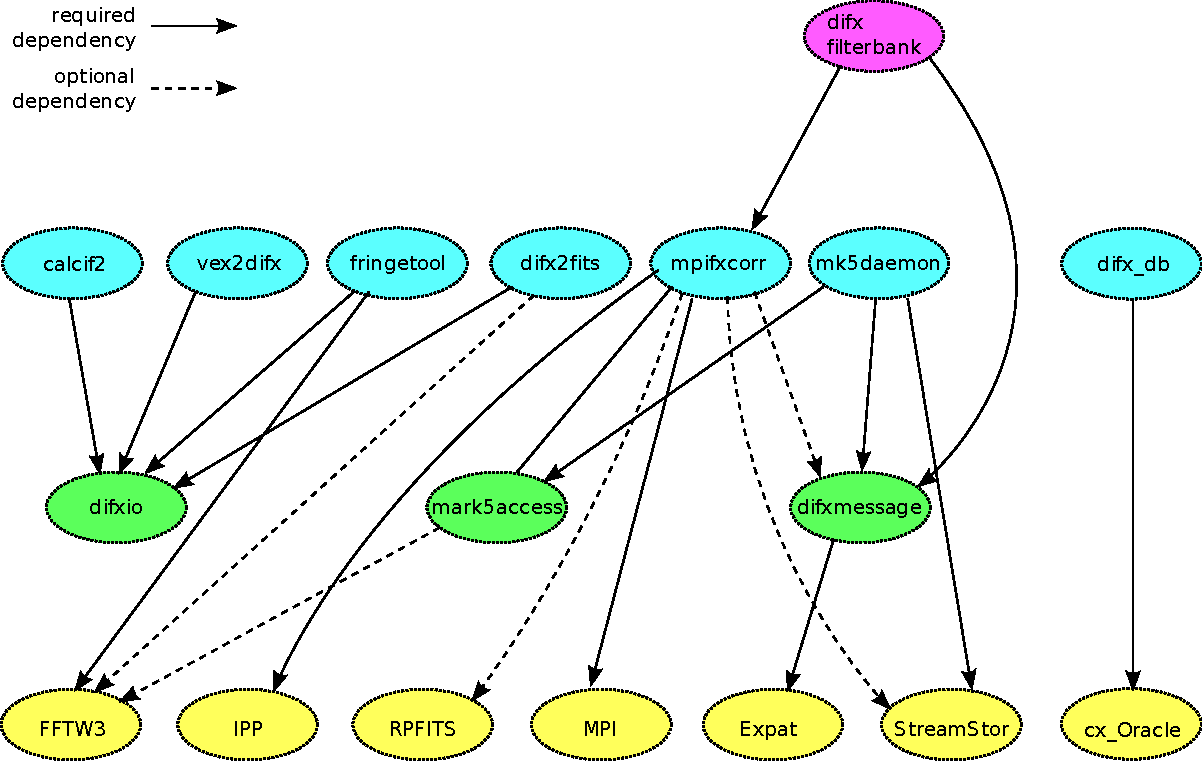
\includegraphics{difxdependency}}
\caption[dependencies]{
{\em A diagram illustrating the required and optional packages and their installation dependencies.}
\label{fig:dependencies}
}
\end{center}
\end{figure}

The {\tt make install} steps may require root permission, depending on the {\em prefixdir} you have chosen.
If so, become root before each {\tt make install}.  
It is advisable not to compile code as root.
Be wary of errors along the way; occasional warnings may be issued, but if the building proceeds, things are probably okay.
Please report any build issues to {\tt wbrisken@nrao.edu}. 
Be warned that these instructions may change.

All of the subversion repositories below point to a {\tt difx-1.5} tagged release of the repository.
This is in order to provide a relatively stable source tree that allows development to continue on the main development branch (called {\tt trunk}).
In order to check out code that is on this development branch, simply replace {\tt tags/difx-1.5} with {\tt trunk} in all of the {\tt svn} commands below.
{\em Caveat emptor: } the {\tt trunk} branch code may at any time refuse to compile, be unstable, lack documentation, or produce incorrect results.
Don't let this stop you if you are an intrepid developer or want to see ongoing development in progress!

%If you do not have SVN access, {\tt .tar.gz} files are available from \url{http://www.aoc.nrao.edu/~wbrisken/difx-1.5/}.








% expat -----------------------------------------------------------------------

\subsubsection{expat} \label{sec:expat}

Expat is a standard library for simple XML parsing.
By default it is installed on almost all Linux distributions.
If it is not, it can be downloaded and installed based on instructions that can be found at its web page:
\url{http://expat.sourceforge.net/} .








% cx_Oracle -------------------------------------------------------------------

\subsubsection{cx\_Oracle} \label{sec:cxOracle}

In the implementation of the VLBA-DiFX operations plans, with the exception of the {\tt DOI}, all of the access to VLBA database is done using python programs that employ the cx\_Oracle library.
This library directly talks to Oracle databases; its use in Python makes for nearly effortless database interfacing.
To install:
\begin{enumerate}
\item Download the latest source distribution from \url{http://cx-oracle.sourceforge.net/} (ver.\ 5.1.2 as of this writing)
\item Decompress the contents into perhaps {\em sourcedir}; enter the newly created directory
\item Run {\tt python setup.py build}
\item Make sure install directory exists:  {\tt mkdir -p \$DIFXROOT/lib/python2.4/site-packages}
\item Run {\tt python setup.py install --prefix=\$DIFXROOT}
\end{enumerate}

\noindent
Notes:
\begin{enumerate}
\item You should substitute {\tt python2.4} with the string appropriate for your python version.
\item {\tt lib} may need to be replaced with {\tt lib64} in the path above.
\item Proper installation can be tested by running {\tt python} and typing {\tt import cx\_Oracle} at the {\tt >>>} prompt.
If another prompt is given without any ``ImportError'' message, then it should be installed properly.
\item The {\tt setup.py} file from version 5.1.2 seems to have an incompatibility with RedHat Enterprise Linux 6 (and there may be other varients of this incompatibility).
Inserting {\tt extraCompileArgs.append("-D\_\_USE\_XOPEN2K8")} at a logical outer-level location around line 200 seems to fix this problem.
\end{enumerate}






% openmpi ---------------------------------------------------------------------

\subsubsection{OpenMPI} \label{sec:mpi}

The core of DiFX uses Message Passing Interface (MPI) for inter-node communication.
Many MPI libraries exist; we choose to use OpenMPI as it is simple to install, runs well, and appears to have good community support.
\begin{enumerate}
\item Download the latest source distribution from \url{http://www.open-mpi.org/} (ver.\ 1.4.2 as of this writing)
\item Decompress the contents into perhaps {\em sourcedir}; enter the newly created directory
\item {\tt ./configure --prefix=}{\em openmpiprefix} where {\em openmpiprefix} could be the same as {\em prefixdir}, but does not have to be.
\item Run {\tt make} and finally {\tt make install} to put the parts where they belong.
\end{enumerate}








% ipp -------------------------------------------------------------------------

\subsubsection{Intel Performance Primitives} \label{sec:ipp}

Intel CPUs support an increasing variety of vector math instructions.  
The Intel Performance Primitives (IPP) makes exploiting these capabilities on any recent generation CPU simple.
An inexpensive license must be purchased to make use of these.
More information can be found on \url{http://www.intel.com}.

Once installed, set environment variable {\tt IPPROOT} to point to its install prefix, which will look something like:
{\tt /home/swc/difx/intel/ipp/6.0.2.076/ia32}; you want to choose the directory containing {\tt lib}, {\tt include}, etc.
Remember to change this in your shell initialization file as well.
This install directory should be visible to all nodes in the cluster.








% fftw ------------------------------------------------------------------------

\subsubsection{FFTW} \label{sec:fftw}

The FFTs performed by {\tt mpifxcorr} are done using the Intel Performance Primitives library, but FFTs done in an optional piece of{\tt difx2fits} and the utility {\tt m5spec} that comes with mark5access use FFTW, a standard, fast, freely available FFT library.
This library is probably installed for you with any modern Linux distribution, but you should check to make sure it is recent enough; version 3.0 and up are supported, but version 3.1.2 or newer is recommended.
If this library is not installed and the extra functionality that requires FFTW is not installed, follow the instructions below:
\begin{enumerate}
\item Download the latest source distribution from \url{http://www.fftw.org} (ver.\ 3.1.2 as of this writing)
\item Decompress the contents into perhaps {\em sourcedir}; enter the newly created directory
\item {\tt ./configure --prefix=}{\em prefixdir}
\item Run {\tt make} and finally {\tt make install} to put the parts where they belong.
\end{enumerate}








% streamstor ---------------------------------------------- INCOMPLETE --------









% difxio ----------------------------------------------------------------------

\subsubsection{difxio} \label{sec:difxio}

Parsing of text files can be tedious.  
The library difxio makes parsing difx-style files simple.
It also contains functionality to completely represent the configuration of a DiFX correlation, simplifying format conversions.
To install:
\begin{enumerate}
\item {\tt cd} {\em sourcedir}
\item Check out the subversion repository: \\
{\tt svn co }\url{https://svn.atnf.csiro.au/difx/libraries/difxio/branches/difx-1.5}{\tt\ difxio} \\
{\em Note: don't forget the {\tt difxio} at the end of the line!}
\item Enter the new directory {\tt cd difxio}
\item View the {\tt README} file.  
Note the next 5 instructions only need to be done once in this directory, even after updating the repository.
You can {\tt man} the commands if you want to know what they do.
\item {\tt aclocal}  
\item {\tt libtoolize --copy --force}
\item {\tt autoconf}
\item {\tt autoheader}
\item {\tt automake -a} 
\item Generate the Makefile: {\tt ./configure --prefix=}{\em prefixdir}
\item Build it: {\tt make}
\item Install it: {\tt make install}
\end{enumerate}

You can test for successful installation by running {\tt pkg-config --cflags difxio}.  
If you get a sensible answer, things are probably good.
If you wish to upgrade the installation:
\begin{enumerate}
\item {\tt cd} {\em sourcedir}{\tt /difxio}
\item Get updates from the repository: {\tt svn update}
\item Build it: {\tt make}
\item Install it: {\tt make install}
\end{enumerate}

Note that doing this upgrade may break other packages that depend on it, such as {\tt difx2fits} and {\tt calcif}, forcing a recompile of these programs.









% difxmessage -----------------------------------------------------------------

\subsubsection{difxmessage {\small $\mathrm{(optional)}$}} \label{sec:difxmessage}

The library difxmessage implements in the C language XML generation and parsing and multicast sending and receiving functionality that is used for communication between various parts of the DiFX system.
See \S\ref{sec:xml} for details on the XML documents supported.
The communication model is based on that of the EVLA.
This package is optional; if not built, you will not be able to use {\tt mk5daemon} or any program packaged with it, or {\tt genmachines}.
To install:
\begin{enumerate}
\item {\tt cd} {\em sourcedir}
\item Check out the subversion repository: \\
{\tt svn co }\url{https://svn.atnf.csiro.au/difx/libraries/difxmessage/branches/difx-1.5}{\tt\ difxmessage}
\item Enter the new directory {\tt cd difxmessage}
\item View the {\tt README} file.  
Note the next 5 instructions only need to be done once in this directory, even after updating the repository.
You can {\tt man} the commands if you want to know what they do.
\item {\tt aclocal}  
\item {\tt libtoolize --copy --force}
\item {\tt autoconf}
\item {\tt autoheader}
\item {\tt automake -a} 
\item Generate the Makefile: {\tt ./configure --prefix=}{\em prefixdir}
\item Build it: {\tt make}
\item Install it: {\tt make install}
\end{enumerate}

You can test for successful installation by running {\tt pkg-config --cflags difxmessage}.  
If you get a sensible answer, things are probably good.
If you wish to upgrade the installation:
\begin{enumerate}
\item {\tt cd} {\em sourcedir}{\tt /difxio}
\item Get updates from the repository: {\tt svn update}
\item Build it: {\tt make}
\item Install it: {\tt make install}
\end{enumerate}

Note that doing this upgrade may break other packages that depend on it, such as {\tt mpifxcorr} and {\tt mk5daemon}, forcing a recompile of these programs.









% mark5access -----------------------------------------------------------------

\subsubsection{mark5access} \label{sec:m5a}

mark5access is a library to parse various VLBI baseband data formats, including Mark4, VLBA, and Mark5B, with other formats to be added.
This is needed to decode these various formats from within mpifxcorr.
To install:
\begin{enumerate}
\item {\tt cd} {\em sourcedir}
\item Check out the subversion repository: \\
{\tt svn co }\url{https://svn.atnf.csiro.au/difx/libraries/mark5access/branches/difx-1.5}{\tt\ mark5access}
\item Enter the new directory {\tt cd mark5access}
\item View the {\tt README} file.  
Note the next 5 instructions only need to be done once in this directory, even after updating the repository.
\item {\tt aclocal}  
\item {\tt libtoolize --copy --force}
\item {\tt autoconf}
\item {\tt autoheader}
\item {\tt automake -a} 
\item Generate the Makefile: {\tt ./configure --prefix=}{\em prefixdir}
\item Build it: {\tt make}
\item Install it: {\tt make install}
\end{enumerate}

You can test for successful installation by running {\tt pkg-config --cflags mark5access}.  
If you get a sensible answer, things are probably good.
If you wish to upgrade the installation:
\begin{enumerate}
\item {\tt cd} {\em sourcedir}{\tt /mark5access}
\item Get updates from the repository: {\tt svn update}
\item Build it: {\tt make}
\item Install it: {\tt make install}
\end{enumerate}

Note that doing this upgrade may break other packages that depend on it, such as {\tt mpifxcorr}, forcing a recompile of these programs.









% mpifxcorr -------------------------------------------------------------------

\subsubsection{mpifxcorr}

The core of the DiFX software correlator is {\tt mpifxcorr}.  
Installation and running this program requires that MPI (\S\ref{sec:mpi}), IPP (\S\ref{sec:ipp}), difxio and mark5access all be installed.
To install:
\begin{enumerate}
\item {\tt cd} {\em sourcedir}
\item Check out the subversion repository: \\
{\tt svn co }\url{https://svn.atnf.csiro.au/difx/mpifxcorr/branches/difx-1.5}{\tt\ mpifxcorr}
\item Enter the new directory {\tt cd mpifxcorr}
\item View the {\tt README} file.  
Note the next 4 instructions only need to be done once in this directory, even after updating the repository.
\item {\tt aclocal}
\item {\tt autoconf}
\item {\tt autoheader}
\item {\tt automake -a}
\item Generate the Makefile: {\tt ./configure --prefix=}{\em prefixdir} {\tt CXX=}{\em openmpiprefix}{\tt /bin/mpicxx}
\item Build it: {\tt make}
\item Install it: {\tt make install}
\end{enumerate}

If successfully installed, the command {\tt which mpifxcorr} should return {\em prefixdir}{\tt /bin/mpifxcorr}.
If you wish to upgrade the installation:
\begin{enumerate}
\item {\tt cd} {\em sourcedir}{\tt /mpifxcorr}
\item Get updates from the repository: {\tt svn update}
\item Build it: {\tt make}
\item Install it: {\tt make install}
\end{enumerate}








% calcserver ------------------------------------------------------------------

\subsubsection{calcserver} \label{sec:calcserver}

The Goddard Space Flight Center CALC package version 9.1 is used to calculate the delay models needed for time-alignment of the raw data.
This software is wrapped in a program that exposes the capabilities of CALC via a Remote Procedure Call (RPC) and this program runs as a server.
An environment variable {\tt CALC\_SERVER} should be set that contains the name of the computer running {\tt calcserver}.
Within DiFX, the only program that makes use of this server is {\tt calcif2} (\S\ref{sec:calcif2}).
To install:
\begin{enumerate}
\item {\tt cd} {\em sourcedir}
\item Check out the subversion repository: \\
{\tt svn co }\url{https://svn.atnf.csiro.au/difx/applications/calcserver/branches/difx-1.5}{\tt\ calcserver}
\item Enter the new directory {\tt cd calcserver}
\item View the {\tt README} file.
\item {\tt aclocal}
\item {\tt libtoolize --copy --force}
\item {\tt autoconf}
\item {\tt automake -a}
\item Generate the Makefile: {\tt ./configure --prefix=}{\em prefixdir}
\item Build it: {\tt make}
\item Install it: {\tt make install}
\end{enumerate}

Since {\tt calcserver} is a single-instance program that is always running as a service, it is usually convenient to have this program start upon boot of the calcserver host.
The calcserver distribution produces a file called {\em srcDir}{\em calcserver/init.d/calcserver} that can be copied (as root) to the system {\tt /etc/init.d} directory.
After doing so, the {\tt /etc/rc.d} directories may need to be updated to run this script at the right time.
On RedHat systems, this is done with:

\noindent
{\tt /sbin/chkconfig --add calcserver}








% calcif2 ---------------------------------------------------------------------

\subsubsection{calcif2} \label{package:calcif2}

The {\tt calcif2} package contains several programs that are useful for DiFX input file creation and managing correlation, most notably {\tt calcif2} .
Note that this package used to be called {\em job2difx}.
To install:
\begin{enumerate}
\item {\tt cd} {\em sourcedir}
\item Check out the subversion repository: \\
{\tt svn co }\url{https://svn.atnf.csiro.au/difx/utilities/branches/difx-1.5/calcif2}{\tt\ calcif2}
\item Enter the new directory {\tt cd calcif2}
\item View the {\tt README} file.  
Note the next 4 instructions only need to be done once in this directory, even after updating the repository.
\item {\tt aclocal}
\item {\tt autoconf}
\item {\tt autoheader}
\item {\tt automake -a}
\item Generate the Makefile: {\tt ./configure --prefix=}{\em prefixdir}
\item Build it: {\tt make}
\item Install it: {\tt make install}
\end{enumerate}

If successfully installed, the command {\tt which calcif2} should return {\em prefixdir}{\tt /bin/calcif2}.
Several other programs should also be installed, including: {\tt genmachines}, {\tt getjobs}, {\tt jobdisks}, {\tt joblist}, {\tt jobstatus}, {\tt difxsniff}, {\tt mk5take}, {\tt mk5return}, and {\tt vlog}.
If you wish to upgrade the installation:
\begin{enumerate}
\item {\tt cd} {\em sourcedir}{\tt /calcif2}
\item Get updates from the repository: {\tt svn update}
\item Build it: {\tt make}
\item Install it: {\tt make install}
\end{enumerate}







% difx2fits -------------------------------------------------------------------

\subsubsection{difx2fits}

The initial NRAO adaptation of DiFX is designed to interface as seamlessly as possible into our existing infrastructure and habits.
This means generation of FITS-IDI output files for compliance with AIPS.
The program {\tt difx2fits} takes many input files (see Fig.~\ref{fig:block}) and produces a FITS file for every DiFX input file.
To install:
\begin{enumerate}
\item {\tt cd} {\em sourcedir}
\item Check out the subversion repository: \\
{\tt svn co }\url{https://svn.atnf.csiro.au/difx/applications/difx2fits/branches/difx-1.5}{\tt\ difx2fits}
\item Enter the new directory {\tt cd difx2fits}
\item View the {\tt README} file.  
Note the next 4 instructions only need to be done once in this directory, even after updating the repository.
\item {\tt aclocal}
\item {\tt autoconf}
\item {\tt autoheader}
\item {\tt automake -a}
\item Generate the Makefile: {\tt ./configure --prefix=}{\em prefixdir}
\item Build it: {\tt make}
\item Install it: {\tt make install}
\end{enumerate}

If successfully installed, the command {\tt which difx2fits} should return {\em prefixdir}{\tt /bin/difx2fits}.
If you wish to upgrade the installation:
\begin{enumerate}
\item {\tt cd} {\em sourcedir}{\tt /difx2fits}
\item Get updates from the repository: {\tt svn update}
\item Build it: {\tt make}
\item Install it: {\tt make install}
\end{enumerate}








% mk5daemon -------------------------------------------------------------------

\subsubsection{mk5daemon {\small $\mathrm{(optional)}$}} 

The optional package {\tt mk5daemon} relies on package {\tt difxmessage} and is only really needed for installations requiring playback off Mark5 modules.
Root permission is required for proper installation and running of this program.
See \S\ref{sec:mk5daemon} for a description of the main program, {\tt mk5daemon}, that comes with this package.
Other useful scripts are included here.
To install:
\begin{enumerate}
\item {\tt cd} {\em sourcedir}
\item Check out the subversion repository: \\
{\tt svn co }\url{https://svn.atnf.csiro.au/difx/applications/mk5daemon/branches/difx-1.5}{\tt\ mk5daemon}
\item Enter the new directory {\tt cd mk5daemon}
\item View the {\tt README} file.  
Note the next 4 instructions only need to be done once in this directory, even after updating the repository.
\item {\tt aclocal}
\item {\tt autoconf}
\item {\tt autoheader}
\item {\tt automake -a}
\item Generate the Makefile: {\tt ./configure --prefix=}{\em prefixdir}
\item Build it: {\tt make}
\item Install it: {\tt make install}
\item Ensure that this program starts at boot.
This requires the following to occur on each computer in the cluster.
Note that the instructions may vary depending on your operating system.
The program is likely to get started before NSF is started, so {\tt mk5daemon} should be installed locally on each compute in the cluster.
On each machine, run as root: {\tt cp }{\em prefixdir}{\tt /bin/mk5daemon} {\em localdir} {\tt ; echo }{\em localdir}{\tt /mk5daemon >> /etc/rc.local} .
Here {\em localdir} is a directory on the particular machine, such as {\tt /usr/bin}
This only needs to be run
\end{enumerate}

If successfully installed, the command {\tt which mk5daemon} should return {\em prefixdir}{\tt /bin/mk5daemon}.
If you wish to upgrade the installation:
\begin{enumerate}
\item {\tt cd} {\em sourcedir}{\tt /mk5daemon}
\item Get updates from the repository: {\tt svn update}
\item Build it: {\tt make}
\item Install it: {\tt make install}
\item Copy it to the local disk (as root): {\tt cp -f }{\em prefixdir}{\tt /bin/mk5daemon} {\em localdir}
\end{enumerate}








% vex2difx --------------------------------------------------------------------

\subsubsection{vex2difx}

The {\tt vex2difx} program aims to convert any legal, complete vex format experiment description file into {\tt .input} and {\tt .calc} files for use with DiFX.
To install:
\begin{enumerate}
\item {\tt cd} {\em sourcedir}
\item Check out the subversion repository: \\
{\tt svn co }\url{https://svn.atnf.csiro.au/difx/applications/vex2difx/branches/difx-1.5}{\tt\ vex2difx}
\item Enter the new directory {\tt cd vex2difx}
\item View the {\tt README} file.  
Note the next 4 instructions only need to be done once in this directory, even after updating the repository.
\item {\tt aclocal}
\item {\tt autoconf}
\item {\tt autoheader}
\item {\tt automake -a}
\item Generate the Makefile: {\tt ./configure --prefix=}{\em prefixdir}
\item Build it: {\tt make}
\item Install it: {\tt make install}
\end{enumerate}

If successfully installed, the command {\tt which vex2difx} should return {\em prefixdir}{\tt /bin/vex2difx}.
If you wish to upgrade the installation:
\begin{enumerate}
\item {\tt cd} {\em sourcedir}{\tt /vex2difx}
\item Get updates from the repository: {\tt svn update}
\item Build it: {\tt make}
\item Install it: {\tt make install}
\end{enumerate}









% difx_db ------------------------------------------------- NRAO ONLY ---------

\subsubsection{difx\_db {\small $\mathrm{(NRAO\ only)}$}}

Package {\tt difx\_db} contains several scripts that either make direct connection to the VLBA database or require site-specific access.
Thus, this package is not available from the standard DiFX repositories.
If any programs in this package seem especially appropriate for use at a correlator other than the VLBA DiFX correlator, please let me know and I'll see what I can do to make it more generally useful.
To install:
\begin{enumerate}
\item {\tt cd} {\em sourcedir}
\item Check out the subversion repository
\item Enter the new directory {\tt cd difx\_db}
\item View the {\tt README} file.  
Note the next 4 instructions only need to be done once in this directory, even after updating the repository.
\item {\tt aclocal}
\item {\tt autoconf}
\item {\tt automake -a}
\item Generate the Makefile: {\tt ./configure --prefix=}{\em prefixdir}
\item Build it: {\tt make}
\item Install it: {\tt make install}
\item ({\em as root}) Change file ownership: {\tt chown root} {\em prefixdir}{\tt /e2ecopy}
\item ({\em as root}) Set UID: {\tt chmod +s} {\em prefixdir}{\tt /e2ecopy}
\end{enumerate}

If successfully installed, the command {\tt which difxqueue} should return {\em prefixdir}{\tt /bin/difxqueue}.
If you wish to upgrade the installation:
\begin{enumerate}
\item {\tt cd} {\em sourcedir}{\tt /vex2difx}
\item Get updates from the repository: {\tt svn update}
\item Build it: {\tt make}
\item Install it: {\tt make install}
\item ({\em as root}) Change file ownership: {\tt chown root} {\em prefixdir}{\tt /e2ecopy}
\item ({\em as root}) Set UID: {\tt chmod +s} {\em prefixdir}{\tt /e2ecopy}
\end{enumerate}


\section{Acknowledgements}

Many people have helped in significant ways to get DiFX adapted for the VLBA:
Craig West for getting me interested in software correlators to begin with; 
Adam Deller for writing DiFX and helping adapt it to the needs of the VLBA; 
Steve Tingay and Matthew Bailes for allowing/encouraging Adam to write DiFX and helping support some of my travel in Australia;
Chris Phillips, John Morgan, Helge Rottmann, Mark Kettenis, Olaf Wucknitz, Mariano Muscas, Geoff Crew, John Spitzak, Roger Cappallo, Walter Max-Moerbeck and Dmitry Baksheev for contributing code, bug reports, bug fixes, and ideas;
Maria Davis, Roopesh Ojha and Dan Veillette for performing careful comparisons with geodetic data;
Walter Alef for hosting the first and second DiFX workshops in 2007 and 2008 at MPIfR, Bonn;
Miguel Guerra for helping define the database and XML structures and his work on the operator interface;
Claire Chandler and Jon Romney/ for project oversight, test planning, advice, and voices of reason;
Steven Durand for acquisition of computer and Mark5 equipment;
David Boboltz, Geoff Bower, Mark Claussen, Vivek Dhawan, Alan Fey, Vincent Fish, Ed Fomalont, David Gordon, Miller Goss, Yuri Kovalev, Matt Lister, Enno Middelberg, James Miller-Jones, Amy Mioduszewski, Leonid Petrov, Mark Reid, Lor\'{a}nt Sjouwerman and Craig Walker for working directly with or examinating the output of DiFX and providing valuable feedback;
Cormac Reynolds for maintaining the Difx wiki which hosts valuable information, hosting the third DiFX workshop in Perth, and providing lots of code;
Jan Wagner, Sergei Pogrebenko, Alexander Neidhardt, Martin Ettl, Jongsoo Kim and Randall Wayth for reporting bugs;
Eric Greisen for making AIPS work well with DiFX output;
John Benson for working with me to get data into the VLBA archive;
James Robnett, Nicole Geiger, David Halstead and Pat van Buskirk for substantial computer and networking support and useful discussions on clustering;
Mike Titus and Arthur Niell for providing test data;
Leonia Kogan for carefully reviewing the conventions used;
Pete Whiteis and Bill Sahr for contributing to helper programs;
Ken Owens and Cindy Gold at Conduant for helping resolve Mark5 issues;
Doug Gerrard, Bob McGoldrick, Adrian Rascon, K. Scott Rowe, Lothar Dahlmayer, and Jeff Long for assembling and maintaining the VLBA DiFX correlator;
Juan Cordova, Paul Dyer, Lisa Foley, Heidi Medlin, Ken Hartley, Alan Kerr, Jim Ogle, Paul Padilla, Peggy Perley, Tony Perreault, Betty Ragan, Meri Stanley and Anthony Sowinski for providing operations assistance;
Chet Ruszczyk, Dan Smythe, and John Ball for extensive Mark5 support over the last decade
and
Emma Goldberg for helping me work around the idiosyncrasies of \LaTeX \ and convince it to typeset this document.
If I left anyone of this list that should be there, and there are probably several of you in that category, I apologize --- let me know and I'll make sure to add you for the next version's document.


\begin{thebibliography}{}
\bibitem{opsplan}
	{\it VLBA-DIFX Operations Plan}, Brisken, W., 2009, VLBA Sensitivity Upgrade Memo 25, \url{http://www.vlba.nrao.edu/memos/sensi/sensimemo25.pdf}
\bibitem{difx}
	{\it DiFX: A software correlator for very long baseline interferometry using multi-processor computing environments}, Deller, A.~T., Tingay, S.~J., Bailes, M. \& West, C., 2007, PASP 119, 318, \url{http://xxx.lanl.gov/abs/astro-ph/0702141}
\bibitem{aips102}
	{\it DiFX2: A more flexible, efficient, robust and powerful software correlator}, A.\ T.\ Deller, W.\ F.\ Brisken, C.\ J.\ Phillips, J.\ Morgan, W.\ Alef, R.\ Cappallo, E.\ Middelberg, J.\ Romney, H.\ Rottmann, S.\ J.\ Tingay, R.\ Wayth, 2011, PASP, 123, 275, \url{http://arxiv.org/abs/1101.0885}
	{\it The FITS Interferometry Data Interchange Format}, Flatters, C., AIPS Memo 102, \url{ftp://ftp.aoc.nrao.edu/pub/software/aips/TEXT/PUBL/AIPSMEMO102.PS}
\bibitem{aips114}
	{\it The FITS Interferometry Data Interchange Convention}, Greisen, E., AIPS Memo 114r {\it in prep}, \url{ftp://ftp.aoc.nrao.edu/pub/software/aips/TEXT/PUBL/AIPSMEM114.PDF}
\bibitem{mark5-81}
	{\it Specification for enhanced Mark 5 module directory}, Whitney, A., et al., \url{http://www.haystack.mit.edu/tech/vlbi/mark5/mark5_memos/081.pdf}
\bibitem{mark5-100}
	{\it  	Mark5 User Directory Formats}, Ruszczyk, C.A., Eldering, B.\ \& Verkouter, H., \url{http://www.haystack.mit.edu/tech/vlbi/mark5/mark5_memos/100.pdf}
\bibitem{sci12}
	{\it Summary of the b-factor for the VLBA FX correlator}, Kogan, L., VLBA Scientific Memo 12, \url{http://www.vlba.nrao.edu/memos/sci/sci12memo.pdf}
\bibitem{tempo}
	{\it Tempo}, \url{http://www.atnf.csiro.au/research/pulsar/tempo/}
\bibitem{jira}
	{\it JIRA}, \url{http://bugs.aoc.nrao.edu}
\bibitem{ngas}
	{\it NGAS}, \url{http://www.eso.org/projects/dfs/dfs-shared/web/ngas/}
%\bibitem{doi}
%	{\it Difx Operator Interface Users Guide}, Guerra, M., {\bf Coming soon!}
\bibitem{vex}
	{\it VEX parameter definitions}, \url{http://www.haystack.mit.edu/tech/vlbi/mark5/vex.html}
\bibitem{wiki}
	{\it DiFX Developer Pages}, \url{http://cira.ivec.org/dokuwiki/doku.php/difx/start}
\end{thebibliography}


\end{document}

